\documentclass[twoside]{book}

% Packages required by doxygen
\usepackage{fixltx2e}
\usepackage{calc}
\usepackage{doxygen}
\usepackage[export]{adjustbox} % also loads graphicx
\usepackage{graphicx}
\usepackage[utf8]{inputenc}
\usepackage{makeidx}
\usepackage{multicol}
\usepackage{multirow}
\PassOptionsToPackage{warn}{textcomp}
\usepackage{textcomp}
\usepackage[nointegrals]{wasysym}
\usepackage[table]{xcolor}

% Font selection
\usepackage[T1]{fontenc}
\usepackage[scaled=.90]{helvet}
\usepackage{courier}
\usepackage{amssymb}
\usepackage{sectsty}
\renewcommand{\familydefault}{\sfdefault}
\allsectionsfont{%
  \fontseries{bc}\selectfont%
  \color{darkgray}%
}
\renewcommand{\DoxyLabelFont}{%
  \fontseries{bc}\selectfont%
  \color{darkgray}%
}
\newcommand{\+}{\discretionary{\mbox{\scriptsize$\hookleftarrow$}}{}{}}

% Page & text layout
\usepackage{geometry}
\geometry{%
  a4paper,%
  top=2.5cm,%
  bottom=2.5cm,%
  left=2.5cm,%
  right=2.5cm%
}
\tolerance=750
\hfuzz=15pt
\hbadness=750
\setlength{\emergencystretch}{15pt}
\setlength{\parindent}{0cm}
\setlength{\parskip}{3ex plus 2ex minus 2ex}
\makeatletter
\renewcommand{\paragraph}{%
  \@startsection{paragraph}{4}{0ex}{-1.0ex}{1.0ex}{%
    \normalfont\normalsize\bfseries\SS@parafont%
  }%
}
\renewcommand{\subparagraph}{%
  \@startsection{subparagraph}{5}{0ex}{-1.0ex}{1.0ex}{%
    \normalfont\normalsize\bfseries\SS@subparafont%
  }%
}
\makeatother

% Headers & footers
\usepackage{fancyhdr}
\pagestyle{fancyplain}
\fancyhead[LE]{\fancyplain{}{\bfseries\thepage}}
\fancyhead[CE]{\fancyplain{}{}}
\fancyhead[RE]{\fancyplain{}{\bfseries\leftmark}}
\fancyhead[LO]{\fancyplain{}{\bfseries\rightmark}}
\fancyhead[CO]{\fancyplain{}{}}
\fancyhead[RO]{\fancyplain{}{\bfseries\thepage}}
\fancyfoot[LE]{\fancyplain{}{}}
\fancyfoot[CE]{\fancyplain{}{}}
\fancyfoot[RE]{\fancyplain{}{\bfseries\scriptsize Generated by Doxygen }}
\fancyfoot[LO]{\fancyplain{}{\bfseries\scriptsize Generated by Doxygen }}
\fancyfoot[CO]{\fancyplain{}{}}
\fancyfoot[RO]{\fancyplain{}{}}
\renewcommand{\footrulewidth}{0.4pt}
\renewcommand{\chaptermark}[1]{%
  \markboth{#1}{}%
}
\renewcommand{\sectionmark}[1]{%
  \markright{\thesection\ #1}%
}

% Indices & bibliography
\usepackage{natbib}
\usepackage[titles]{tocloft}
\setcounter{tocdepth}{3}
\setcounter{secnumdepth}{5}
\makeindex

% Hyperlinks (required, but should be loaded last)
\usepackage{ifpdf}
\ifpdf
  \usepackage[pdftex,pagebackref=true]{hyperref}
\else
  \usepackage[ps2pdf,pagebackref=true]{hyperref}
\fi
\hypersetup{%
  colorlinks=true,%
  linkcolor=blue,%
  citecolor=blue,%
  unicode%
}

% Custom commands
\newcommand{\clearemptydoublepage}{%
  \newpage{\pagestyle{empty}\cleardoublepage}%
}

\usepackage{caption}
\captionsetup{labelsep=space,justification=centering,font={bf},singlelinecheck=off,skip=4pt,position=top}

%===== C O N T E N T S =====

\begin{document}

% Titlepage & ToC
\hypersetup{pageanchor=false,
             bookmarksnumbered=true,
             pdfencoding=unicode
            }
\pagenumbering{roman}
\begin{titlepage}
\vspace*{7cm}
\begin{center}%
{\Large My Project }\\
\vspace*{1cm}
{\large Generated by Doxygen 1.8.11}\\
\end{center}
\end{titlepage}
\clearemptydoublepage
\tableofcontents
\clearemptydoublepage
\pagenumbering{arabic}
\hypersetup{pageanchor=true}

%--- Begin generated contents ---
\chapter{Namespace Index}
\section{Namespace List}
Here is a list of all documented namespaces with brief descriptions\+:\begin{DoxyCompactList}
\item\contentsline{section}{\hyperlink{namespacedue}{due} \\*Hwlib implementation for the Arduino Due }{\pageref{namespacedue}}{}
\end{DoxyCompactList}

\chapter{Hierarchical Index}
\section{Class Hierarchy}
This inheritance list is sorted roughly, but not completely, alphabetically\+:\begin{DoxyCompactList}
\item \contentsline{section}{hwlib\+:\+:\+\_\+boolalpha}{\pageref{structhwlib_1_1__boolalpha}}{}
\item \contentsline{section}{hwlib\+:\+:\+\_\+flush}{\pageref{structhwlib_1_1__flush}}{}
\item \contentsline{section}{hwlib\+:\+:\+\_\+left}{\pageref{structhwlib_1_1__left}}{}
\item \contentsline{section}{hwlib\+:\+:\+\_\+right}{\pageref{structhwlib_1_1__right}}{}
\item \contentsline{section}{hwlib\+:\+:\+\_\+setbase}{\pageref{structhwlib_1_1__setbase}}{}
\item \contentsline{section}{hwlib\+:\+:\+\_\+showbase}{\pageref{structhwlib_1_1__showbase}}{}
\item \contentsline{section}{hwlib\+:\+:\+\_\+showpos}{\pageref{structhwlib_1_1__showpos}}{}
\item \contentsline{section}{due\+:\+:ad\+\_\+pin\+\_\+info\+\_\+type}{\pageref{structdue_1_1ad__pin__info__type}}{}
\item \contentsline{section}{hwlib\+:\+:adc}{\pageref{classhwlib_1_1adc}}{}
\begin{DoxyCompactList}
\item \contentsline{section}{due\+:\+:pin\+\_\+adc}{\pageref{classdue_1_1pin__adc}}{}
\end{DoxyCompactList}
\item \contentsline{section}{hwlib\+:\+:color}{\pageref{classhwlib_1_1color}}{}
\item \contentsline{section}{hwlib\+:\+:dac}{\pageref{classhwlib_1_1dac}}{}
\item \contentsline{section}{hwlib\+:\+:drawable}{\pageref{classhwlib_1_1drawable}}{}
\begin{DoxyCompactList}
\item \contentsline{section}{hwlib\+:\+:circle}{\pageref{classhwlib_1_1circle}}{}
\item \contentsline{section}{hwlib\+:\+:line}{\pageref{classhwlib_1_1line}}{}
\end{DoxyCompactList}
\item \contentsline{section}{hwlib\+:\+:font}{\pageref{classhwlib_1_1font}}{}
\begin{DoxyCompactList}
\item \contentsline{section}{hwlib\+:\+:font\+\_\+default\+\_\+16x16}{\pageref{classhwlib_1_1font__default__16x16}}{}
\item \contentsline{section}{hwlib\+:\+:font\+\_\+default\+\_\+8x8}{\pageref{classhwlib_1_1font__default__8x8}}{}
\end{DoxyCompactList}
\item \contentsline{section}{hwlib\+:\+:i2c\+\_\+bus}{\pageref{classhwlib_1_1i2c__bus}}{}
\begin{DoxyCompactList}
\item \contentsline{section}{hwlib\+:\+:i2c\+\_\+bus\+\_\+bit\+\_\+banged\+\_\+scl\+\_\+sda}{\pageref{classhwlib_1_1i2c__bus__bit__banged__scl__sda}}{}
\end{DoxyCompactList}
\item \contentsline{section}{hwlib\+:\+:image}{\pageref{classhwlib_1_1image}}{}
\begin{DoxyCompactList}
\item \contentsline{section}{hwlib\+:\+:image\+\_\+16x16}{\pageref{classhwlib_1_1image__16x16}}{}
\item \contentsline{section}{hwlib\+:\+:image\+\_\+8x8}{\pageref{classhwlib_1_1image__8x8}}{}
\end{DoxyCompactList}
\item \contentsline{section}{hwlib\+:\+:istream}{\pageref{classhwlib_1_1istream}}{}
\begin{DoxyCompactList}
\item \contentsline{section}{hwlib\+:\+:keypad$<$ N $>$}{\pageref{classhwlib_1_1keypad}}{}
\end{DoxyCompactList}
\item \contentsline{section}{hwlib\+:\+:location}{\pageref{classhwlib_1_1location}}{}
\item \contentsline{section}{hwlib\+:\+:matrix\+\_\+of\+\_\+switches}{\pageref{classhwlib_1_1matrix__of__switches}}{}
\item \contentsline{section}{hwlib\+:\+:ostream}{\pageref{classhwlib_1_1ostream}}{}
\begin{DoxyCompactList}
\item \contentsline{section}{hwlib\+:\+:console}{\pageref{classhwlib_1_1console}}{}
\begin{DoxyCompactList}
\item \contentsline{section}{hwlib\+:\+:hd44780}{\pageref{classhwlib_1_1hd44780}}{}
\item \contentsline{section}{hwlib\+:\+:window\+\_\+ostream}{\pageref{classhwlib_1_1window__ostream}}{}
\end{DoxyCompactList}
\end{DoxyCompactList}
\item \contentsline{section}{hwlib\+:\+:pcf8591}{\pageref{classhwlib_1_1pcf8591}}{}
\item \contentsline{section}{hwlib\+:\+:pin\+\_\+in}{\pageref{classhwlib_1_1pin__in}}{}
\begin{DoxyCompactList}
\item \contentsline{section}{due\+:\+:pin\+\_\+in}{\pageref{classdue_1_1pin__in}}{}
\item \contentsline{section}{hwlib\+:\+:\+\_\+pin\+\_\+in\+\_\+dummy\+\_\+class}{\pageref{classhwlib_1_1__pin__in__dummy__class}}{}
\end{DoxyCompactList}
\item \contentsline{section}{hwlib\+:\+:pin\+\_\+in\+\_\+out}{\pageref{classhwlib_1_1pin__in__out}}{}
\begin{DoxyCompactList}
\item \contentsline{section}{due\+:\+:pin\+\_\+in\+\_\+out}{\pageref{classdue_1_1pin__in__out}}{}
\item \contentsline{section}{hwlib\+:\+:\+\_\+pin\+\_\+in\+\_\+out\+\_\+dummy\+\_\+class}{\pageref{classhwlib_1_1__pin__in__out__dummy__class}}{}
\end{DoxyCompactList}
\item \contentsline{section}{hwlib\+:\+:pin\+\_\+oc}{\pageref{classhwlib_1_1pin__oc}}{}
\begin{DoxyCompactList}
\item \contentsline{section}{due\+:\+:pin\+\_\+oc}{\pageref{classdue_1_1pin__oc}}{}
\item \contentsline{section}{hwlib\+:\+:\+\_\+pin\+\_\+oc\+\_\+dummy\+\_\+class}{\pageref{classhwlib_1_1__pin__oc__dummy__class}}{}
\end{DoxyCompactList}
\item \contentsline{section}{hwlib\+:\+:pin\+\_\+out}{\pageref{classhwlib_1_1pin__out}}{}
\begin{DoxyCompactList}
\item \contentsline{section}{due\+:\+:d2\+\_\+36k\+Hz}{\pageref{classdue_1_1d2__36k_hz}}{}
\item \contentsline{section}{due\+:\+:pin\+\_\+out}{\pageref{classdue_1_1pin__out}}{}
\item \contentsline{section}{hwlib\+:\+:\+\_\+pin\+\_\+out\+\_\+dummy\+\_\+class}{\pageref{classhwlib_1_1__pin__out__dummy__class}}{}
\end{DoxyCompactList}
\item \contentsline{section}{hwlib\+:\+:port\+\_\+in}{\pageref{classhwlib_1_1port__in}}{}
\begin{DoxyCompactList}
\item \contentsline{section}{hwlib\+:\+:port\+\_\+in\+\_\+from\+\_\+pins}{\pageref{classhwlib_1_1port__in__from__pins}}{}
\item \contentsline{section}{hwlib\+:\+:port\+\_\+in\+\_\+invert}{\pageref{classhwlib_1_1port__in__invert}}{}
\end{DoxyCompactList}
\item \contentsline{section}{hwlib\+:\+:port\+\_\+in\+\_\+out}{\pageref{classhwlib_1_1port__in__out}}{}
\begin{DoxyCompactList}
\item \contentsline{section}{hwlib\+:\+:port\+\_\+in\+\_\+out\+\_\+from\+\_\+pins}{\pageref{classhwlib_1_1port__in__out__from__pins}}{}
\item \contentsline{section}{hwlib\+:\+:port\+\_\+in\+\_\+out\+\_\+invert}{\pageref{classhwlib_1_1port__in__out__invert}}{}
\end{DoxyCompactList}
\item \contentsline{section}{hwlib\+:\+:port\+\_\+oc}{\pageref{classhwlib_1_1port__oc}}{}
\begin{DoxyCompactList}
\item \contentsline{section}{hwlib\+:\+:pcf8574a}{\pageref{classhwlib_1_1pcf8574a}}{}
\item \contentsline{section}{hwlib\+:\+:port\+\_\+oc\+\_\+from\+\_\+pins}{\pageref{classhwlib_1_1port__oc__from__pins}}{}
\item \contentsline{section}{hwlib\+:\+:port\+\_\+oc\+\_\+invert}{\pageref{classhwlib_1_1port__oc__invert}}{}
\end{DoxyCompactList}
\item \contentsline{section}{hwlib\+:\+:port\+\_\+out}{\pageref{classhwlib_1_1port__out}}{}
\begin{DoxyCompactList}
\item \contentsline{section}{hwlib\+:\+:hc595}{\pageref{classhwlib_1_1hc595}}{}
\item \contentsline{section}{hwlib\+:\+:port\+\_\+out\+\_\+from\+\_\+pins}{\pageref{classhwlib_1_1port__out__from__pins}}{}
\item \contentsline{section}{hwlib\+:\+:port\+\_\+out\+\_\+invert}{\pageref{classhwlib_1_1port__out__invert}}{}
\end{DoxyCompactList}
\item \contentsline{section}{sam3xa}{\pageref{structsam3xa}}{}
\item \contentsline{section}{hwlib\+:\+:setfill}{\pageref{structhwlib_1_1setfill}}{}
\item \contentsline{section}{hwlib\+:\+:setw}{\pageref{structhwlib_1_1setw}}{}
\item \contentsline{section}{hwlib\+:\+:spi\+\_\+bus}{\pageref{classhwlib_1_1spi__bus}}{}
\begin{DoxyCompactList}
\item \contentsline{section}{hwlib\+:\+:spi\+\_\+bus\+\_\+bit\+\_\+banged\+\_\+sclk\+\_\+mosi\+\_\+miso}{\pageref{classhwlib_1_1spi__bus__bit__banged__sclk__mosi__miso}}{}
\end{DoxyCompactList}
\item \contentsline{section}{hwlib\+:\+:window}{\pageref{classhwlib_1_1window}}{}
\begin{DoxyCompactList}
\item \contentsline{section}{hwlib\+:\+:glcd\+\_\+5510}{\pageref{classhwlib_1_1glcd__5510}}{}
\item \contentsline{section}{hwlib\+:\+:glcd\+\_\+oled}{\pageref{classhwlib_1_1glcd__oled}}{}
\item \contentsline{section}{hwlib\+:\+:glcd\+\_\+oled\+\_\+buffered}{\pageref{classhwlib_1_1glcd__oled__buffered}}{}
\item \contentsline{section}{hwlib\+:\+:window\+\_\+invert}{\pageref{classhwlib_1_1window__invert}}{}
\item \contentsline{section}{hwlib\+:\+:window\+\_\+part}{\pageref{classhwlib_1_1window__part}}{}
\end{DoxyCompactList}
\end{DoxyCompactList}

\chapter{Class Index}
\section{Class List}
Here are the classes, structs, unions and interfaces with brief descriptions\+:\begin{DoxyCompactList}
\item\contentsline{section}{\hyperlink{classrtos_1_1channel}{rtos\+::channel$<$ T, S\+I\+Z\+E $>$} \\*Waitable data queue }{\pageref{classrtos_1_1channel}}{}
\item\contentsline{section}{\hyperlink{classrtos_1_1channel__base}{rtos\+::channel\+\_\+base} \\*Rtos private implementation class }{\pageref{classrtos_1_1channel__base}}{}
\item\contentsline{section}{\hyperlink{classrtos_1_1clock}{rtos\+::clock} \\*Free-\/running clock, ticks at a fixed frequency }{\pageref{classrtos_1_1clock}}{}
\item\contentsline{section}{\hyperlink{classcoroutine}{coroutine$<$ N $>$} }{\pageref{classcoroutine}}{}
\item\contentsline{section}{\hyperlink{classcoroutine_3_010_01_4}{coroutine$<$ 0 $>$} \\*Coroutine class }{\pageref{classcoroutine_3_010_01_4}}{}
\item\contentsline{section}{\hyperlink{classcoroutine__context}{coroutine\+\_\+context} }{\pageref{classcoroutine__context}}{}
\item\contentsline{section}{\hyperlink{classrtos_1_1event}{rtos\+::event} \\*Set of things that can happen, or a thing that has happened }{\pageref{classrtos_1_1event}}{}
\item\contentsline{section}{\hyperlink{classrtos_1_1flag}{rtos\+::flag} \\*Basic synchronisation mechanism }{\pageref{classrtos_1_1flag}}{}
\item\contentsline{section}{\hyperlink{classrtos_1_1mailbox}{rtos\+::mailbox$<$ T $>$} \\*Synchronously handing over of a data item }{\pageref{classrtos_1_1mailbox}}{}
\item\contentsline{section}{\hyperlink{classrtos_1_1mailbox__base}{rtos\+::mailbox\+\_\+base} \\*Rtos private implementation class }{\pageref{classrtos_1_1mailbox__base}}{}
\item\contentsline{section}{\hyperlink{classrtos_1_1mutex}{rtos\+::mutex} \\*Mutual execlusion semaphore }{\pageref{classrtos_1_1mutex}}{}
\item\contentsline{section}{\hyperlink{classrtos_1_1pool}{rtos\+::pool$<$ T $>$} \\*Place to store and rectrieve data, no built-\/in synchronisation }{\pageref{classrtos_1_1pool}}{}
\item\contentsline{section}{\hyperlink{classrtos_1_1pool__base}{rtos\+::pool\+\_\+base} \\*Rtos private implementation class }{\pageref{classrtos_1_1pool__base}}{}
\item\contentsline{section}{\hyperlink{classrtos}{rtos} \\*Static class, namespace-\/like container for R\+T\+OS declarations }{\pageref{classrtos}}{}
\item\contentsline{section}{\hyperlink{classrtos_1_1task}{rtos\+::task$<$ N $>$} }{\pageref{classrtos_1_1task}}{}
\item\contentsline{section}{\hyperlink{classrtos_1_1task__base}{rtos\+::task\+\_\+base} \\*Independent thread of execution }{\pageref{classrtos_1_1task__base}}{}
\item\contentsline{section}{\hyperlink{classrtos_1_1timer}{rtos\+::timer} \\*One-\/shot timer }{\pageref{classrtos_1_1timer}}{}
\item\contentsline{section}{\hyperlink{classrtos_1_1waitable}{rtos\+::waitable} \\*Abstract thing that a task can wait for }{\pageref{classrtos_1_1waitable}}{}
\end{DoxyCompactList}

\chapter{File Index}
\section{File List}
Here is a list of all documented files with brief descriptions\+:\begin{DoxyCompactList}
\item\contentsline{section}{\hyperlink{coroutine_8hpp}{coroutine.\+hpp} }{\pageref{coroutine_8hpp}}{}
\item\contentsline{section}{\hyperlink{rtos_8hpp}{rtos.\+hpp} }{\pageref{rtos_8hpp}}{}
\item\contentsline{section}{\hyperlink{switch__to_8hpp}{switch\+\_\+to.\+hpp} }{\pageref{switch__to_8hpp}}{}
\end{DoxyCompactList}

\chapter{Namespace Documentation}
\hypertarget{namespacedue}{}\section{due Namespace Reference}
\label{namespacedue}\index{due@{due}}


hwlib implementation for the Arduino Due  


\subsection*{Classes}
\begin{DoxyCompactItemize}
\item 
struct \hyperlink{structdue_1_1ad__pin__info__type}{ad\+\_\+pin\+\_\+info\+\_\+type}
\item 
class \hyperlink{classdue_1_1d2__36k_hz}{d2\+\_\+36k\+Hz}
\item 
class \hyperlink{classdue_1_1pin__adc}{pin\+\_\+adc}
\begin{DoxyCompactList}\small\item\em \hyperlink{classdue_1_1pin__adc}{pin\+\_\+adc} implementation for a A\+T\+S\+A\+M3\+X8E \end{DoxyCompactList}\item 
class \hyperlink{classdue_1_1pin__in}{pin\+\_\+in}
\begin{DoxyCompactList}\small\item\em \hyperlink{classdue_1_1pin__in}{pin\+\_\+in} implementation for a A\+T\+S\+A\+M3\+X8E \end{DoxyCompactList}\item 
class \hyperlink{classdue_1_1pin__in__out}{pin\+\_\+in\+\_\+out}
\begin{DoxyCompactList}\small\item\em \hyperlink{classdue_1_1pin__in__out}{pin\+\_\+in\+\_\+out} implementation for a A\+T\+S\+A\+M3\+X8E \end{DoxyCompactList}\item 
class \hyperlink{classdue_1_1pin__oc}{pin\+\_\+oc}
\begin{DoxyCompactList}\small\item\em \hyperlink{classdue_1_1pin__oc}{pin\+\_\+oc} implementation for a A\+T\+S\+A\+M3\+X8E \end{DoxyCompactList}\item 
class \hyperlink{classdue_1_1pin__out}{pin\+\_\+out}
\begin{DoxyCompactList}\small\item\em \hyperlink{classdue_1_1pin__out}{pin\+\_\+out} implementation for a A\+T\+S\+A\+M3\+X8E \end{DoxyCompactList}\end{DoxyCompactItemize}
\subsection*{Enumerations}
\begin{DoxyCompactItemize}
\item 
enum \hyperlink{namespacedue_a8ffa3ec309934ff9db34317e504bcc92}{pins} \{ \\*
{\bfseries d0}, 
{\bfseries d1}, 
{\bfseries d2}, 
{\bfseries d3}, 
\\*
{\bfseries d4}, 
{\bfseries d5}, 
{\bfseries d6}, 
{\bfseries d7}, 
\\*
{\bfseries d8}, 
{\bfseries d9}, 
{\bfseries d10}, 
{\bfseries d11}, 
\\*
{\bfseries d12}, 
{\bfseries d13}, 
{\bfseries d14}, 
{\bfseries d15}, 
\\*
{\bfseries d16}, 
{\bfseries d17}, 
{\bfseries d18}, 
{\bfseries d19}, 
\\*
{\bfseries d20}, 
{\bfseries d21}, 
{\bfseries d22}, 
{\bfseries d23}, 
\\*
{\bfseries d24}, 
{\bfseries d25}, 
{\bfseries d26}, 
{\bfseries d27}, 
\\*
{\bfseries d28}, 
{\bfseries d29}, 
{\bfseries d30}, 
{\bfseries d31}, 
\\*
{\bfseries d32}, 
{\bfseries d33}, 
{\bfseries d34}, 
{\bfseries d35}, 
\\*
{\bfseries d36}, 
{\bfseries d37}, 
{\bfseries d38}, 
{\bfseries d39}, 
\\*
{\bfseries d40}, 
{\bfseries d41}, 
{\bfseries d42}, 
{\bfseries d43}, 
\\*
{\bfseries d44}, 
{\bfseries d45}, 
{\bfseries d46}, 
{\bfseries d47}, 
\\*
{\bfseries d48}, 
{\bfseries d49}, 
{\bfseries d50}, 
{\bfseries d51}, 
\\*
{\bfseries d52}, 
{\bfseries d53}, 
{\bfseries a0}, 
{\bfseries a1}, 
\\*
{\bfseries a2}, 
{\bfseries a3}, 
{\bfseries a4}, 
{\bfseries a5}, 
\\*
{\bfseries a6}, 
{\bfseries a7}, 
{\bfseries a8}, 
{\bfseries a9}, 
\\*
{\bfseries a10}, 
{\bfseries a11}, 
{\bfseries dac0}, 
{\bfseries dac1}, 
\\*
{\bfseries canrx}, 
{\bfseries cantx}, 
{\bfseries scl}, 
{\bfseries sda}, 
\\*
{\bfseries scl1}, 
{\bfseries sda1}, 
{\bfseries tx}, 
{\bfseries rx}, 
\\*
{\bfseries led}, 
{\bfseries sck}, 
{\bfseries miso}, 
{\bfseries mosi}, 
\\*
{\bfseries cs0}, 
{\bfseries cs1}
 \}\begin{DoxyCompactList}\small\item\em Arduino Due G\+P\+IO pin names. \end{DoxyCompactList}
\item 
enum \hyperlink{namespacedue_a5ecc98d40585c91eabbfb14f71bd7d4c}{ad\+\_\+pins} \{ \\*
{\bfseries a0}, 
{\bfseries a1}, 
{\bfseries a2}, 
{\bfseries a3}, 
\\*
{\bfseries a4}, 
{\bfseries a5}, 
{\bfseries a6}, 
{\bfseries a7}, 
\\*
{\bfseries a8}, 
{\bfseries a9}, 
{\bfseries a10}, 
{\bfseries a11}
 \}\begin{DoxyCompactList}\small\item\em Arduino Due pin names. \end{DoxyCompactList}
\end{DoxyCompactItemize}
\subsection*{Functions}
\begin{DoxyCompactItemize}
\item 
Pio \& {\bfseries \+\_\+\+\_\+attribute\+\_\+\+\_\+} ((weak)) port\+\_\+registers(int port)\hypertarget{namespacedue_a691468d1eaea9eb36a06b94e7c27d6fa}{}\label{namespacedue_a691468d1eaea9eb36a06b94e7c27d6fa}

\item 
long long int \hyperlink{hwlib-defines_8hpp_a04be4340016df60d6636c1d1c6d94fc9}{H\+W\+L\+I\+B\+\_\+\+W\+E\+AK} \hyperlink{namespacedue_aed372aa18d1261d874f74642952d4b53}{now\+\_\+ticks} ()\hypertarget{namespacedue_aed372aa18d1261d874f74642952d4b53}{}\label{namespacedue_aed372aa18d1261d874f74642952d4b53}

\begin{DoxyCompactList}\small\item\em returns the number of ticks since some fixed starting point \end{DoxyCompactList}\item 
long long int \hyperlink{hwlib-defines_8hpp_a04be4340016df60d6636c1d1c6d94fc9}{H\+W\+L\+I\+B\+\_\+\+W\+E\+AK} \hyperlink{namespacedue_a763b16adccc73515e1d463402e05fd52}{now\+\_\+us} ()\hypertarget{namespacedue_a763b16adccc73515e1d463402e05fd52}{}\label{namespacedue_a763b16adccc73515e1d463402e05fd52}

\begin{DoxyCompactList}\small\item\em returns the number of us since some fixed starting point \end{DoxyCompactList}\end{DoxyCompactItemize}
\subsection*{Variables}
\begin{DoxyCompactItemize}
\item 
const long long int \hyperlink{namespacedue_af3604632f92cd8ee84f9ba4ca8d51349}{ticks\+\_\+per\+\_\+us} = 84\hypertarget{namespacedue_af3604632f92cd8ee84f9ba4ca8d51349}{}\label{namespacedue_af3604632f92cd8ee84f9ba4ca8d51349}

\begin{DoxyCompactList}\small\item\em the number of ticks per us \end{DoxyCompactList}\end{DoxyCompactItemize}


\subsection{Detailed Description}
hwlib implementation for the Arduino Due 

 and (sotware) U\+A\+RT output for the Arduino Due (A\+T\+S\+A\+M3\+X8E chip). The first wait call configures the chip to run at 12 M\+Hz, from its internal (calibrated) RC oscillator.

The port and pin parameters to the constructors of the pin classes can either use to the A\+T\+S\+A\+M3\+X8E ports and pins, or the Arduino names.

The Due has an on-\/board orange L\+ED connected to port 1 pin 27.

The chip runs at 3.\+3 Volt and that is the level on its IO pins.



The A\+T\+S\+A\+M3\+X8E chip has a watchdog system that is enabled by default. If left alone, the watchdog will reset the chip after a short time. To prevent this, all Due applications start with these lines\+: 
\begin{DoxyCode}
\textcolor{comment}{// kill the watchdog}
WDT->WDT\_MR = WDT\_MR\_WDDIS;
\end{DoxyCode}


References\+:
\begin{DoxyItemize}
\item \href{https://www.arduino.cc/en/uploads/Main/arduino-uno-schematic.pdf}{\tt Arduino Due circuit reference diagram} (pdf)
\item \href{http://www.atmel.com/images/atmel-11057-32-bit-cortex-m3-microcontroller-sam3x-sam3a_datasheet.pdf}{\tt A\+T\+S\+A\+M38\+XE datasheet} (pdf) 
\end{DoxyItemize}

\subsection{Enumeration Type Documentation}
\index{due@{due}!ad\+\_\+pins@{ad\+\_\+pins}}
\index{ad\+\_\+pins@{ad\+\_\+pins}!due@{due}}
\subsubsection[{\texorpdfstring{ad\+\_\+pins}{ad_pins}}]{\setlength{\rightskip}{0pt plus 5cm}enum {\bf due\+::ad\+\_\+pins}\hspace{0.3cm}{\ttfamily [strong]}}\hypertarget{namespacedue_a5ecc98d40585c91eabbfb14f71bd7d4c}{}\label{namespacedue_a5ecc98d40585c91eabbfb14f71bd7d4c}


Arduino Due pin names. 

These are the A\+DC pins of an Arduino Due board. \index{due@{due}!pins@{pins}}
\index{pins@{pins}!due@{due}}
\subsubsection[{\texorpdfstring{pins}{pins}}]{\setlength{\rightskip}{0pt plus 5cm}enum {\bf due\+::pins}\hspace{0.3cm}{\ttfamily [strong]}}\hypertarget{namespacedue_a8ffa3ec309934ff9db34317e504bcc92}{}\label{namespacedue_a8ffa3ec309934ff9db34317e504bcc92}


Arduino Due G\+P\+IO pin names. 

These are the pins of an Arduino Due board. Digital pins d0..d13, analog input pins A0..A5, S\+CL, S\+DA, TX (=D1), RX (=D0), L\+ED (=D13), S\+CK (=D13), M\+I\+SO (=D12), M\+O\+SI (=D11), SS (=D10). 
\chapter{Class Documentation}
\hypertarget{structhwlib_1_1__boolalpha}{}\section{hwlib\+:\+:\+\_\+boolalpha Struct Reference}
\label{structhwlib_1_1__boolalpha}\index{hwlib\+::\+\_\+boolalpha@{hwlib\+::\+\_\+boolalpha}}
\subsection*{Public Member Functions}
\begin{DoxyCompactItemize}
\item 
constexpr {\bfseries \+\_\+boolalpha} (bool x)\hypertarget{structhwlib_1_1__boolalpha_a9972ce841479f54863b82332f82ed732}{}\label{structhwlib_1_1__boolalpha_a9972ce841479f54863b82332f82ed732}

\item 
constexpr {\bfseries \+\_\+boolalpha} (bool x)\hypertarget{structhwlib_1_1__boolalpha_a9972ce841479f54863b82332f82ed732}{}\label{structhwlib_1_1__boolalpha_a9972ce841479f54863b82332f82ed732}

\end{DoxyCompactItemize}


The documentation for this struct was generated from the following files\+:\begin{DoxyCompactItemize}
\item 
\hyperlink{hwlib-ostream_01-_01_copy_8hpp}{hwlib-\/ostream -\/ Copy.\+hpp}\item 
\hyperlink{hwlib-ostream_8hpp}{hwlib-\/ostream.\+hpp}\end{DoxyCompactItemize}

\hypertarget{structhwlib_1_1__flush}{}\section{hwlib\+:\+:\+\_\+flush Struct Reference}
\label{structhwlib_1_1__flush}\index{hwlib\+::\+\_\+flush@{hwlib\+::\+\_\+flush}}


The documentation for this struct was generated from the following files\+:\begin{DoxyCompactItemize}
\item 
\hyperlink{hwlib-ostream_01-_01_copy_8hpp}{hwlib-\/ostream -\/ Copy.\+hpp}\item 
\hyperlink{hwlib-ostream_8hpp}{hwlib-\/ostream.\+hpp}\end{DoxyCompactItemize}

\hypertarget{structhwlib_1_1__left}{}\section{hwlib\+:\+:\+\_\+left Struct Reference}
\label{structhwlib_1_1__left}\index{hwlib\+::\+\_\+left@{hwlib\+::\+\_\+left}}


The documentation for this struct was generated from the following files\+:\begin{DoxyCompactItemize}
\item 
\hyperlink{hwlib-ostream_01-_01_copy_8hpp}{hwlib-\/ostream -\/ Copy.\+hpp}\item 
\hyperlink{hwlib-ostream_8hpp}{hwlib-\/ostream.\+hpp}\end{DoxyCompactItemize}

\hypertarget{classhwlib_1_1__pin__in__dummy__class}{}\section{hwlib\+:\+:\+\_\+pin\+\_\+in\+\_\+dummy\+\_\+class Class Reference}
\label{classhwlib_1_1__pin__in__dummy__class}\index{hwlib\+::\+\_\+pin\+\_\+in\+\_\+dummy\+\_\+class@{hwlib\+::\+\_\+pin\+\_\+in\+\_\+dummy\+\_\+class}}


a dummy (do-\/nothing) \hyperlink{classhwlib_1_1pin__in}{pin\+\_\+in}  




{\ttfamily \#include $<$hwlib-\/pin-\/dummies.\+hpp$>$}

Inheritance diagram for hwlib\+:\+:\+\_\+pin\+\_\+in\+\_\+dummy\+\_\+class\+:\begin{figure}[H]
\begin{center}
\leavevmode
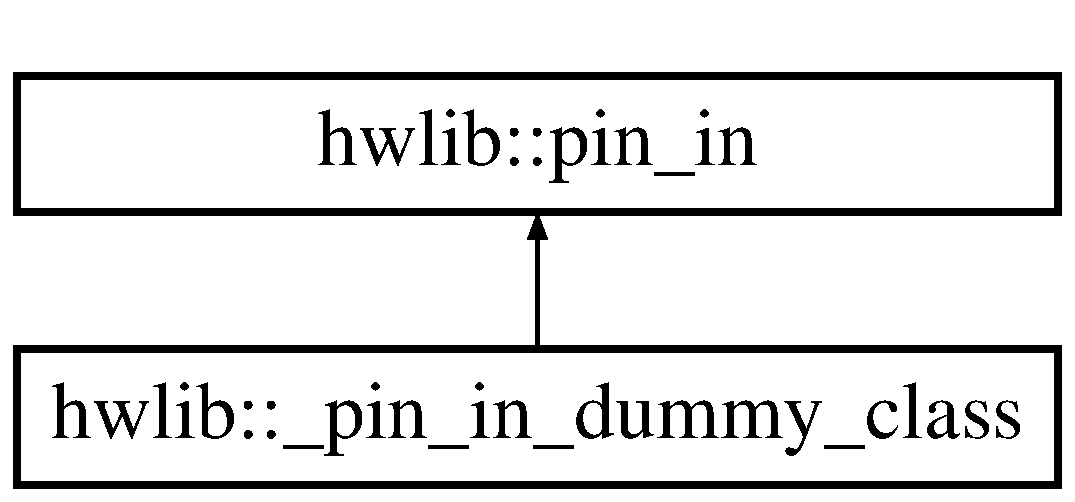
\includegraphics[height=2.000000cm]{classhwlib_1_1__pin__in__dummy__class}
\end{center}
\end{figure}
\subsection*{Public Member Functions}
\begin{DoxyCompactItemize}
\item 
bool \hyperlink{classhwlib_1_1__pin__in__dummy__class_a2b51c1a0d291cd4414e70504d388c9cb}{get} () override
\begin{DoxyCompactList}\small\item\em read the pin \end{DoxyCompactList}\end{DoxyCompactItemize}


\subsection{Detailed Description}
a dummy (do-\/nothing) \hyperlink{classhwlib_1_1pin__in}{pin\+\_\+in} 

\subsection{Member Function Documentation}
\index{hwlib\+::\+\_\+pin\+\_\+in\+\_\+dummy\+\_\+class@{hwlib\+::\+\_\+pin\+\_\+in\+\_\+dummy\+\_\+class}!get@{get}}
\index{get@{get}!hwlib\+::\+\_\+pin\+\_\+in\+\_\+dummy\+\_\+class@{hwlib\+::\+\_\+pin\+\_\+in\+\_\+dummy\+\_\+class}}
\subsubsection[{\texorpdfstring{get() override}{get() override}}]{\setlength{\rightskip}{0pt plus 5cm}bool hwlib\+::\+\_\+pin\+\_\+in\+\_\+dummy\+\_\+class\+::get (
\begin{DoxyParamCaption}
{}
\end{DoxyParamCaption}
)\hspace{0.3cm}{\ttfamily [inline]}, {\ttfamily [override]}, {\ttfamily [virtual]}}\hypertarget{classhwlib_1_1__pin__in__dummy__class_a2b51c1a0d291cd4414e70504d388c9cb}{}\label{classhwlib_1_1__pin__in__dummy__class_a2b51c1a0d291cd4414e70504d388c9cb}


read the pin 

This function returns the level of the pin. When the pin level is high the value true is returned, when the pin level is low the value false is returned. 

Implements \hyperlink{classhwlib_1_1pin__in_a5cbc123fa14d62c98dd41f7523cf6063}{hwlib\+::pin\+\_\+in}.



The documentation for this class was generated from the following file\+:\begin{DoxyCompactItemize}
\item 
\hyperlink{hwlib-pin-dummies_8hpp}{hwlib-\/pin-\/dummies.\+hpp}\end{DoxyCompactItemize}

\hypertarget{classhwlib_1_1__pin__in__out__dummy__class}{}\section{hwlib\+:\+:\+\_\+pin\+\_\+in\+\_\+out\+\_\+dummy\+\_\+class Class Reference}
\label{classhwlib_1_1__pin__in__out__dummy__class}\index{hwlib\+::\+\_\+pin\+\_\+in\+\_\+out\+\_\+dummy\+\_\+class@{hwlib\+::\+\_\+pin\+\_\+in\+\_\+out\+\_\+dummy\+\_\+class}}


a dummy (do-\/nothing) \hyperlink{classhwlib_1_1pin__in__out}{pin\+\_\+in\+\_\+out}  




{\ttfamily \#include $<$hwlib-\/pin-\/dummies.\+hpp$>$}

Inheritance diagram for hwlib\+:\+:\+\_\+pin\+\_\+in\+\_\+out\+\_\+dummy\+\_\+class\+:\begin{figure}[H]
\begin{center}
\leavevmode
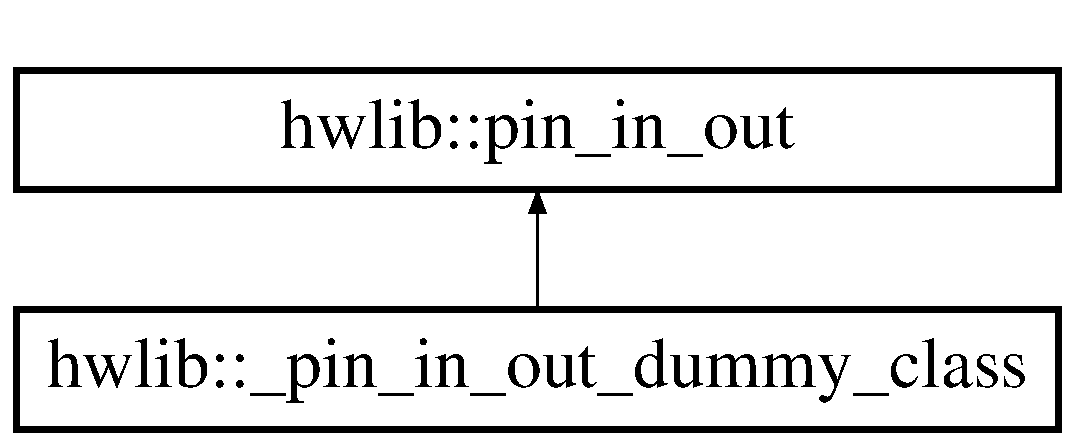
\includegraphics[height=2.000000cm]{classhwlib_1_1__pin__in__out__dummy__class}
\end{center}
\end{figure}
\subsection*{Public Member Functions}
\begin{DoxyCompactItemize}
\item 
void \hyperlink{classhwlib_1_1__pin__in__out__dummy__class_afd92206adb4c05526a84d8e7ff17491c}{set} (bool v) override
\begin{DoxyCompactList}\small\item\em write the pin \end{DoxyCompactList}\item 
bool \hyperlink{classhwlib_1_1__pin__in__out__dummy__class_aa3a8d3f46143f6bb042444dee00c34c6}{get} () override
\begin{DoxyCompactList}\small\item\em read the pin \end{DoxyCompactList}\item 
void \hyperlink{classhwlib_1_1__pin__in__out__dummy__class_a29f385015d361cfa434a625ca8331cd7}{direction\+\_\+set\+\_\+input} () override
\begin{DoxyCompactList}\small\item\em set the direction of a pin to input. \end{DoxyCompactList}\item 
void \hyperlink{classhwlib_1_1__pin__in__out__dummy__class_a551f4d543e9fccd85ad843cbd9258a94}{direction\+\_\+set\+\_\+output} () override
\begin{DoxyCompactList}\small\item\em set the direction of a pin to output \end{DoxyCompactList}\end{DoxyCompactItemize}


\subsection{Detailed Description}
a dummy (do-\/nothing) \hyperlink{classhwlib_1_1pin__in__out}{pin\+\_\+in\+\_\+out} 

\subsection{Member Function Documentation}
\index{hwlib\+::\+\_\+pin\+\_\+in\+\_\+out\+\_\+dummy\+\_\+class@{hwlib\+::\+\_\+pin\+\_\+in\+\_\+out\+\_\+dummy\+\_\+class}!direction\+\_\+set\+\_\+input@{direction\+\_\+set\+\_\+input}}
\index{direction\+\_\+set\+\_\+input@{direction\+\_\+set\+\_\+input}!hwlib\+::\+\_\+pin\+\_\+in\+\_\+out\+\_\+dummy\+\_\+class@{hwlib\+::\+\_\+pin\+\_\+in\+\_\+out\+\_\+dummy\+\_\+class}}
\subsubsection[{\texorpdfstring{direction\+\_\+set\+\_\+input() override}{direction_set_input() override}}]{\setlength{\rightskip}{0pt plus 5cm}void hwlib\+::\+\_\+pin\+\_\+in\+\_\+out\+\_\+dummy\+\_\+class\+::direction\+\_\+set\+\_\+input (
\begin{DoxyParamCaption}
{}
\end{DoxyParamCaption}
)\hspace{0.3cm}{\ttfamily [inline]}, {\ttfamily [override]}, {\ttfamily [virtual]}}\hypertarget{classhwlib_1_1__pin__in__out__dummy__class_a29f385015d361cfa434a625ca8331cd7}{}\label{classhwlib_1_1__pin__in__out__dummy__class_a29f385015d361cfa434a625ca8331cd7}


set the direction of a pin to input. 

Calling this function sets the pin identified by p to input. 

Implements \hyperlink{classhwlib_1_1pin__in__out_a54ce1a5086d3c9e7b868511b1d46acd0}{hwlib\+::pin\+\_\+in\+\_\+out}.

\index{hwlib\+::\+\_\+pin\+\_\+in\+\_\+out\+\_\+dummy\+\_\+class@{hwlib\+::\+\_\+pin\+\_\+in\+\_\+out\+\_\+dummy\+\_\+class}!direction\+\_\+set\+\_\+output@{direction\+\_\+set\+\_\+output}}
\index{direction\+\_\+set\+\_\+output@{direction\+\_\+set\+\_\+output}!hwlib\+::\+\_\+pin\+\_\+in\+\_\+out\+\_\+dummy\+\_\+class@{hwlib\+::\+\_\+pin\+\_\+in\+\_\+out\+\_\+dummy\+\_\+class}}
\subsubsection[{\texorpdfstring{direction\+\_\+set\+\_\+output() override}{direction_set_output() override}}]{\setlength{\rightskip}{0pt plus 5cm}void hwlib\+::\+\_\+pin\+\_\+in\+\_\+out\+\_\+dummy\+\_\+class\+::direction\+\_\+set\+\_\+output (
\begin{DoxyParamCaption}
{}
\end{DoxyParamCaption}
)\hspace{0.3cm}{\ttfamily [inline]}, {\ttfamily [override]}, {\ttfamily [virtual]}}\hypertarget{classhwlib_1_1__pin__in__out__dummy__class_a551f4d543e9fccd85ad843cbd9258a94}{}\label{classhwlib_1_1__pin__in__out__dummy__class_a551f4d543e9fccd85ad843cbd9258a94}


set the direction of a pin to output 

Calling this function sets the pin identified by p to output. 

Implements \hyperlink{classhwlib_1_1pin__in__out_ad08a5f5e9a4c3aadaa7c665b98f2418e}{hwlib\+::pin\+\_\+in\+\_\+out}.

\index{hwlib\+::\+\_\+pin\+\_\+in\+\_\+out\+\_\+dummy\+\_\+class@{hwlib\+::\+\_\+pin\+\_\+in\+\_\+out\+\_\+dummy\+\_\+class}!get@{get}}
\index{get@{get}!hwlib\+::\+\_\+pin\+\_\+in\+\_\+out\+\_\+dummy\+\_\+class@{hwlib\+::\+\_\+pin\+\_\+in\+\_\+out\+\_\+dummy\+\_\+class}}
\subsubsection[{\texorpdfstring{get() override}{get() override}}]{\setlength{\rightskip}{0pt plus 5cm}bool hwlib\+::\+\_\+pin\+\_\+in\+\_\+out\+\_\+dummy\+\_\+class\+::get (
\begin{DoxyParamCaption}
{}
\end{DoxyParamCaption}
)\hspace{0.3cm}{\ttfamily [inline]}, {\ttfamily [override]}, {\ttfamily [virtual]}}\hypertarget{classhwlib_1_1__pin__in__out__dummy__class_aa3a8d3f46143f6bb042444dee00c34c6}{}\label{classhwlib_1_1__pin__in__out__dummy__class_aa3a8d3f46143f6bb042444dee00c34c6}


read the pin 

This function returns the level of the pin. When the pin level is high the value true is returned, when the pin level is low the value false is returned.

Before calling this function the pin direction must have been set to input by calling \hyperlink{classhwlib_1_1__pin__in__out__dummy__class_a29f385015d361cfa434a625ca8331cd7}{direction\+\_\+set\+\_\+input()}. 

Implements \hyperlink{classhwlib_1_1pin__in__out_a298d32c19a8f94b730d34d4496bcf3ae}{hwlib\+::pin\+\_\+in\+\_\+out}.

\index{hwlib\+::\+\_\+pin\+\_\+in\+\_\+out\+\_\+dummy\+\_\+class@{hwlib\+::\+\_\+pin\+\_\+in\+\_\+out\+\_\+dummy\+\_\+class}!set@{set}}
\index{set@{set}!hwlib\+::\+\_\+pin\+\_\+in\+\_\+out\+\_\+dummy\+\_\+class@{hwlib\+::\+\_\+pin\+\_\+in\+\_\+out\+\_\+dummy\+\_\+class}}
\subsubsection[{\texorpdfstring{set(bool v) override}{set(bool v) override}}]{\setlength{\rightskip}{0pt plus 5cm}void hwlib\+::\+\_\+pin\+\_\+in\+\_\+out\+\_\+dummy\+\_\+class\+::set (
\begin{DoxyParamCaption}
\item[{bool}]{x}
\end{DoxyParamCaption}
)\hspace{0.3cm}{\ttfamily [inline]}, {\ttfamily [override]}, {\ttfamily [virtual]}}\hypertarget{classhwlib_1_1__pin__in__out__dummy__class_afd92206adb4c05526a84d8e7ff17491c}{}\label{classhwlib_1_1__pin__in__out__dummy__class_afd92206adb4c05526a84d8e7ff17491c}


write the pin 

This function sets the level of the pin to the value v. A value of true makes the pin high, a value of false makes it low.

Before calling this function the pin direction must have been set to output by calling \hyperlink{classhwlib_1_1__pin__in__out__dummy__class_a551f4d543e9fccd85ad843cbd9258a94}{direction\+\_\+set\+\_\+output()}. 

Implements \hyperlink{classhwlib_1_1pin__in__out_a198c4d27a9783f4c17e8f5dfd9aca6a9}{hwlib\+::pin\+\_\+in\+\_\+out}.



The documentation for this class was generated from the following file\+:\begin{DoxyCompactItemize}
\item 
\hyperlink{hwlib-pin-dummies_8hpp}{hwlib-\/pin-\/dummies.\+hpp}\end{DoxyCompactItemize}

\hypertarget{classhwlib_1_1__pin__oc__dummy__class}{}\section{hwlib\+:\+:\+\_\+pin\+\_\+oc\+\_\+dummy\+\_\+class Class Reference}
\label{classhwlib_1_1__pin__oc__dummy__class}\index{hwlib\+::\+\_\+pin\+\_\+oc\+\_\+dummy\+\_\+class@{hwlib\+::\+\_\+pin\+\_\+oc\+\_\+dummy\+\_\+class}}


a dummy (do-\/nothing) \hyperlink{classhwlib_1_1pin__oc}{pin\+\_\+oc}  




{\ttfamily \#include $<$hwlib-\/pin-\/dummies.\+hpp$>$}

Inheritance diagram for hwlib\+:\+:\+\_\+pin\+\_\+oc\+\_\+dummy\+\_\+class\+:\begin{figure}[H]
\begin{center}
\leavevmode
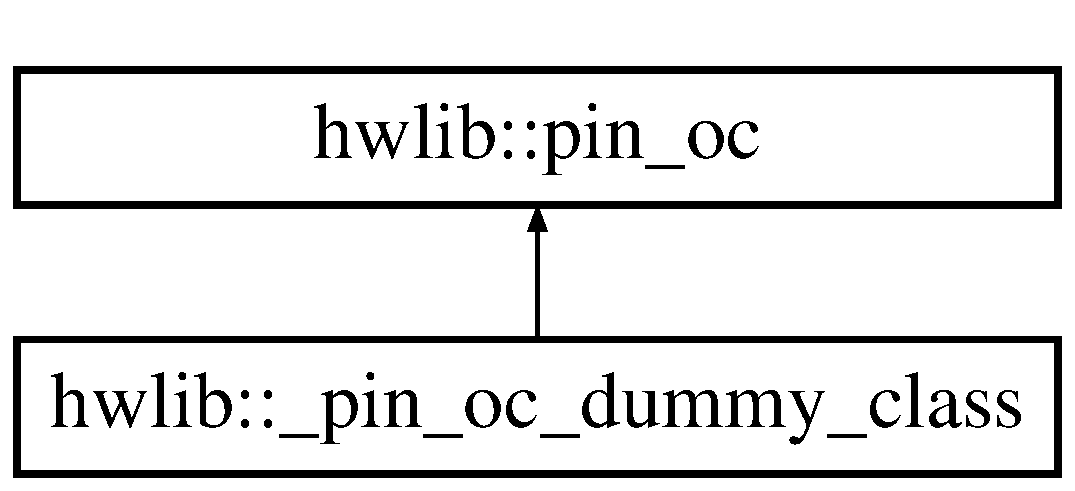
\includegraphics[height=2.000000cm]{classhwlib_1_1__pin__oc__dummy__class}
\end{center}
\end{figure}
\subsection*{Public Member Functions}
\begin{DoxyCompactItemize}
\item 
void \hyperlink{classhwlib_1_1__pin__oc__dummy__class_a10db7f81b4ed0dc0573f039d97c1d69e}{set} (bool v) override
\begin{DoxyCompactList}\small\item\em write the pin \end{DoxyCompactList}\item 
bool \hyperlink{classhwlib_1_1__pin__oc__dummy__class_a06d061b7dd08d290e56969e90d4ff255}{get} () override
\begin{DoxyCompactList}\small\item\em read the pin \end{DoxyCompactList}\end{DoxyCompactItemize}


\subsection{Detailed Description}
a dummy (do-\/nothing) \hyperlink{classhwlib_1_1pin__oc}{pin\+\_\+oc} 

\subsection{Member Function Documentation}
\index{hwlib\+::\+\_\+pin\+\_\+oc\+\_\+dummy\+\_\+class@{hwlib\+::\+\_\+pin\+\_\+oc\+\_\+dummy\+\_\+class}!get@{get}}
\index{get@{get}!hwlib\+::\+\_\+pin\+\_\+oc\+\_\+dummy\+\_\+class@{hwlib\+::\+\_\+pin\+\_\+oc\+\_\+dummy\+\_\+class}}
\subsubsection[{\texorpdfstring{get() override}{get() override}}]{\setlength{\rightskip}{0pt plus 5cm}bool hwlib\+::\+\_\+pin\+\_\+oc\+\_\+dummy\+\_\+class\+::get (
\begin{DoxyParamCaption}
{}
\end{DoxyParamCaption}
)\hspace{0.3cm}{\ttfamily [inline]}, {\ttfamily [override]}, {\ttfamily [virtual]}}\hypertarget{classhwlib_1_1__pin__oc__dummy__class_a06d061b7dd08d290e56969e90d4ff255}{}\label{classhwlib_1_1__pin__oc__dummy__class_a06d061b7dd08d290e56969e90d4ff255}


read the pin 

This function returns the level of the pin. When the pin level is high the value true is returned, when the pin level is low the value false is returned.

This function can be called after set( false ) has been called on the pin, but then the level will read low (false). Call set( true ) to let the line float (presumably pulled high by a pull-\/up resistor) to read the level put on the line by an external device. 

Implements \hyperlink{classhwlib_1_1pin__oc_aa395bf9608ca48ca07dee2f5dc4612bd}{hwlib\+::pin\+\_\+oc}.

\index{hwlib\+::\+\_\+pin\+\_\+oc\+\_\+dummy\+\_\+class@{hwlib\+::\+\_\+pin\+\_\+oc\+\_\+dummy\+\_\+class}!set@{set}}
\index{set@{set}!hwlib\+::\+\_\+pin\+\_\+oc\+\_\+dummy\+\_\+class@{hwlib\+::\+\_\+pin\+\_\+oc\+\_\+dummy\+\_\+class}}
\subsubsection[{\texorpdfstring{set(bool v) override}{set(bool v) override}}]{\setlength{\rightskip}{0pt plus 5cm}void hwlib\+::\+\_\+pin\+\_\+oc\+\_\+dummy\+\_\+class\+::set (
\begin{DoxyParamCaption}
\item[{bool}]{x}
\end{DoxyParamCaption}
)\hspace{0.3cm}{\ttfamily [inline]}, {\ttfamily [override]}, {\ttfamily [virtual]}}\hypertarget{classhwlib_1_1__pin__oc__dummy__class_a10db7f81b4ed0dc0573f039d97c1d69e}{}\label{classhwlib_1_1__pin__oc__dummy__class_a10db7f81b4ed0dc0573f039d97c1d69e}


write the pin 

This function sets the level of the pin to the value v. A value of true makes the pin hihg-\/impedance (presumably pulled high by a pull-\/up resistor), a value of false makes it low. 

Implements \hyperlink{classhwlib_1_1pin__oc_a2165622dad253a423d2fa52cbed7c553}{hwlib\+::pin\+\_\+oc}.



The documentation for this class was generated from the following file\+:\begin{DoxyCompactItemize}
\item 
\hyperlink{hwlib-pin-dummies_8hpp}{hwlib-\/pin-\/dummies.\+hpp}\end{DoxyCompactItemize}

\hypertarget{classhwlib_1_1__pin__out__dummy__class}{}\section{hwlib\+:\+:\+\_\+pin\+\_\+out\+\_\+dummy\+\_\+class Class Reference}
\label{classhwlib_1_1__pin__out__dummy__class}\index{hwlib\+::\+\_\+pin\+\_\+out\+\_\+dummy\+\_\+class@{hwlib\+::\+\_\+pin\+\_\+out\+\_\+dummy\+\_\+class}}


a dummy (do-\/nothing) \hyperlink{classhwlib_1_1pin__out}{pin\+\_\+out}  




{\ttfamily \#include $<$hwlib-\/pin-\/dummies.\+hpp$>$}

Inheritance diagram for hwlib\+:\+:\+\_\+pin\+\_\+out\+\_\+dummy\+\_\+class\+:\begin{figure}[H]
\begin{center}
\leavevmode
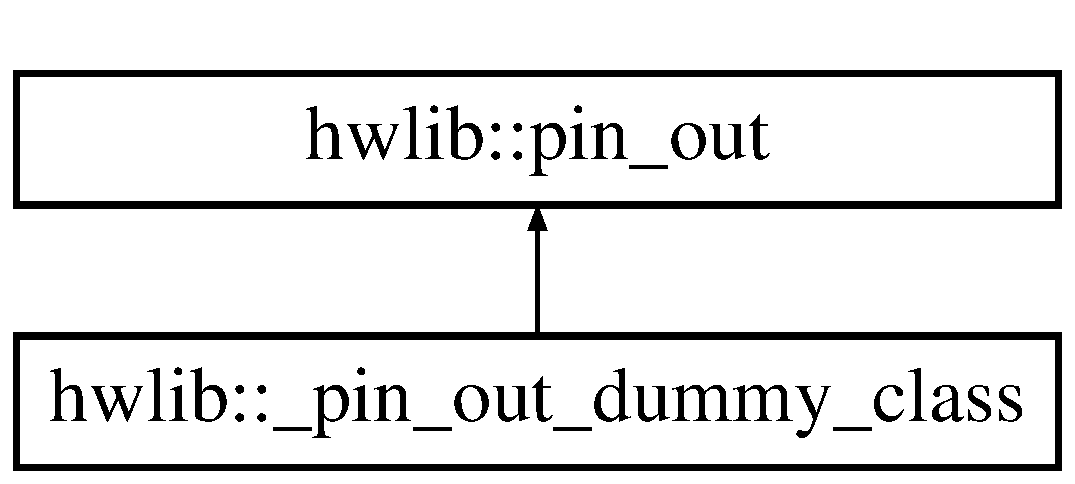
\includegraphics[height=2.000000cm]{classhwlib_1_1__pin__out__dummy__class}
\end{center}
\end{figure}
\subsection*{Public Member Functions}
\begin{DoxyCompactItemize}
\item 
void \hyperlink{classhwlib_1_1__pin__out__dummy__class_a2a1c7ef6046fbf45a92f5036632e4655}{set} (bool v) override
\begin{DoxyCompactList}\small\item\em write the pin \end{DoxyCompactList}\end{DoxyCompactItemize}


\subsection{Detailed Description}
a dummy (do-\/nothing) \hyperlink{classhwlib_1_1pin__out}{pin\+\_\+out} 

\subsection{Member Function Documentation}
\index{hwlib\+::\+\_\+pin\+\_\+out\+\_\+dummy\+\_\+class@{hwlib\+::\+\_\+pin\+\_\+out\+\_\+dummy\+\_\+class}!set@{set}}
\index{set@{set}!hwlib\+::\+\_\+pin\+\_\+out\+\_\+dummy\+\_\+class@{hwlib\+::\+\_\+pin\+\_\+out\+\_\+dummy\+\_\+class}}
\subsubsection[{\texorpdfstring{set(bool v) override}{set(bool v) override}}]{\setlength{\rightskip}{0pt plus 5cm}void hwlib\+::\+\_\+pin\+\_\+out\+\_\+dummy\+\_\+class\+::set (
\begin{DoxyParamCaption}
\item[{bool}]{v}
\end{DoxyParamCaption}
)\hspace{0.3cm}{\ttfamily [inline]}, {\ttfamily [override]}, {\ttfamily [virtual]}}\hypertarget{classhwlib_1_1__pin__out__dummy__class_a2a1c7ef6046fbf45a92f5036632e4655}{}\label{classhwlib_1_1__pin__out__dummy__class_a2a1c7ef6046fbf45a92f5036632e4655}


write the pin 

This function sets the level of the pin to the value v. A value of true makes the pin high, a value of false makes it low. 

Implements \hyperlink{classhwlib_1_1pin__out_af5c3a533f1a00ba973e37e60fb8c08c6}{hwlib\+::pin\+\_\+out}.



The documentation for this class was generated from the following file\+:\begin{DoxyCompactItemize}
\item 
\hyperlink{hwlib-pin-dummies_8hpp}{hwlib-\/pin-\/dummies.\+hpp}\end{DoxyCompactItemize}

\hypertarget{structhwlib_1_1__right}{}\section{hwlib\+:\+:\+\_\+right Struct Reference}
\label{structhwlib_1_1__right}\index{hwlib\+::\+\_\+right@{hwlib\+::\+\_\+right}}


The documentation for this struct was generated from the following files\+:\begin{DoxyCompactItemize}
\item 
\hyperlink{hwlib-ostream_01-_01_copy_8hpp}{hwlib-\/ostream -\/ Copy.\+hpp}\item 
\hyperlink{hwlib-ostream_8hpp}{hwlib-\/ostream.\+hpp}\end{DoxyCompactItemize}

\hypertarget{structhwlib_1_1__setbase}{}\section{hwlib\+:\+:\+\_\+setbase Struct Reference}
\label{structhwlib_1_1__setbase}\index{hwlib\+::\+\_\+setbase@{hwlib\+::\+\_\+setbase}}
\subsection*{Public Member Functions}
\begin{DoxyCompactItemize}
\item 
constexpr {\bfseries \+\_\+setbase} (int x)\hypertarget{structhwlib_1_1__setbase_aacb4b037a7f55889db8afba3c31128a1}{}\label{structhwlib_1_1__setbase_aacb4b037a7f55889db8afba3c31128a1}

\item 
constexpr {\bfseries \+\_\+setbase} (int x)\hypertarget{structhwlib_1_1__setbase_aacb4b037a7f55889db8afba3c31128a1}{}\label{structhwlib_1_1__setbase_aacb4b037a7f55889db8afba3c31128a1}

\end{DoxyCompactItemize}


The documentation for this struct was generated from the following files\+:\begin{DoxyCompactItemize}
\item 
\hyperlink{hwlib-ostream_01-_01_copy_8hpp}{hwlib-\/ostream -\/ Copy.\+hpp}\item 
\hyperlink{hwlib-ostream_8hpp}{hwlib-\/ostream.\+hpp}\end{DoxyCompactItemize}

\hypertarget{structhwlib_1_1__showbase}{}\section{hwlib\+:\+:\+\_\+showbase Struct Reference}
\label{structhwlib_1_1__showbase}\index{hwlib\+::\+\_\+showbase@{hwlib\+::\+\_\+showbase}}
\subsection*{Public Member Functions}
\begin{DoxyCompactItemize}
\item 
constexpr {\bfseries \+\_\+showbase} (bool x)\hypertarget{structhwlib_1_1__showbase_aa9dd5a4b597e34ae374859798a7a3c2d}{}\label{structhwlib_1_1__showbase_aa9dd5a4b597e34ae374859798a7a3c2d}

\item 
constexpr {\bfseries \+\_\+showbase} (bool x)\hypertarget{structhwlib_1_1__showbase_aa9dd5a4b597e34ae374859798a7a3c2d}{}\label{structhwlib_1_1__showbase_aa9dd5a4b597e34ae374859798a7a3c2d}

\end{DoxyCompactItemize}


The documentation for this struct was generated from the following files\+:\begin{DoxyCompactItemize}
\item 
\hyperlink{hwlib-ostream_01-_01_copy_8hpp}{hwlib-\/ostream -\/ Copy.\+hpp}\item 
\hyperlink{hwlib-ostream_8hpp}{hwlib-\/ostream.\+hpp}\end{DoxyCompactItemize}

\hypertarget{structhwlib_1_1__showpos}{}\section{hwlib\+:\+:\+\_\+showpos Struct Reference}
\label{structhwlib_1_1__showpos}\index{hwlib\+::\+\_\+showpos@{hwlib\+::\+\_\+showpos}}
\subsection*{Public Member Functions}
\begin{DoxyCompactItemize}
\item 
constexpr {\bfseries \+\_\+showpos} (bool x)\hypertarget{structhwlib_1_1__showpos_acc9f9e1970e3b70823e9dac74dc942b0}{}\label{structhwlib_1_1__showpos_acc9f9e1970e3b70823e9dac74dc942b0}

\item 
constexpr {\bfseries \+\_\+showpos} (bool x)\hypertarget{structhwlib_1_1__showpos_acc9f9e1970e3b70823e9dac74dc942b0}{}\label{structhwlib_1_1__showpos_acc9f9e1970e3b70823e9dac74dc942b0}

\end{DoxyCompactItemize}


The documentation for this struct was generated from the following files\+:\begin{DoxyCompactItemize}
\item 
\hyperlink{hwlib-ostream_01-_01_copy_8hpp}{hwlib-\/ostream -\/ Copy.\+hpp}\item 
\hyperlink{hwlib-ostream_8hpp}{hwlib-\/ostream.\+hpp}\end{DoxyCompactItemize}

\hypertarget{structdue_1_1ad__pin__info__type}{}\section{due\+:\+:ad\+\_\+pin\+\_\+info\+\_\+type Struct Reference}
\label{structdue_1_1ad__pin__info__type}\index{due\+::ad\+\_\+pin\+\_\+info\+\_\+type@{due\+::ad\+\_\+pin\+\_\+info\+\_\+type}}
\subsection*{Public Attributes}
\begin{DoxyCompactItemize}
\item 
uint8\+\_\+t {\bfseries channel}\hypertarget{structdue_1_1ad__pin__info__type_ae23ba2025e81198f877ccaaa5927a368}{}\label{structdue_1_1ad__pin__info__type_ae23ba2025e81198f877ccaaa5927a368}

\end{DoxyCompactItemize}


The documentation for this struct was generated from the following file\+:\begin{DoxyCompactItemize}
\item 
\hyperlink{hwlib-due_8hpp}{hwlib-\/due.\+hpp}\end{DoxyCompactItemize}

\hypertarget{classhwlib_1_1adc}{}\section{hwlib\+:\+:adc Class Reference}
\label{classhwlib_1_1adc}\index{hwlib\+::adc@{hwlib\+::adc}}


A/D input interface.  




{\ttfamily \#include $<$hwlib-\/adc.\+hpp$>$}

Inheritance diagram for hwlib\+:\+:adc\+:\begin{figure}[H]
\begin{center}
\leavevmode
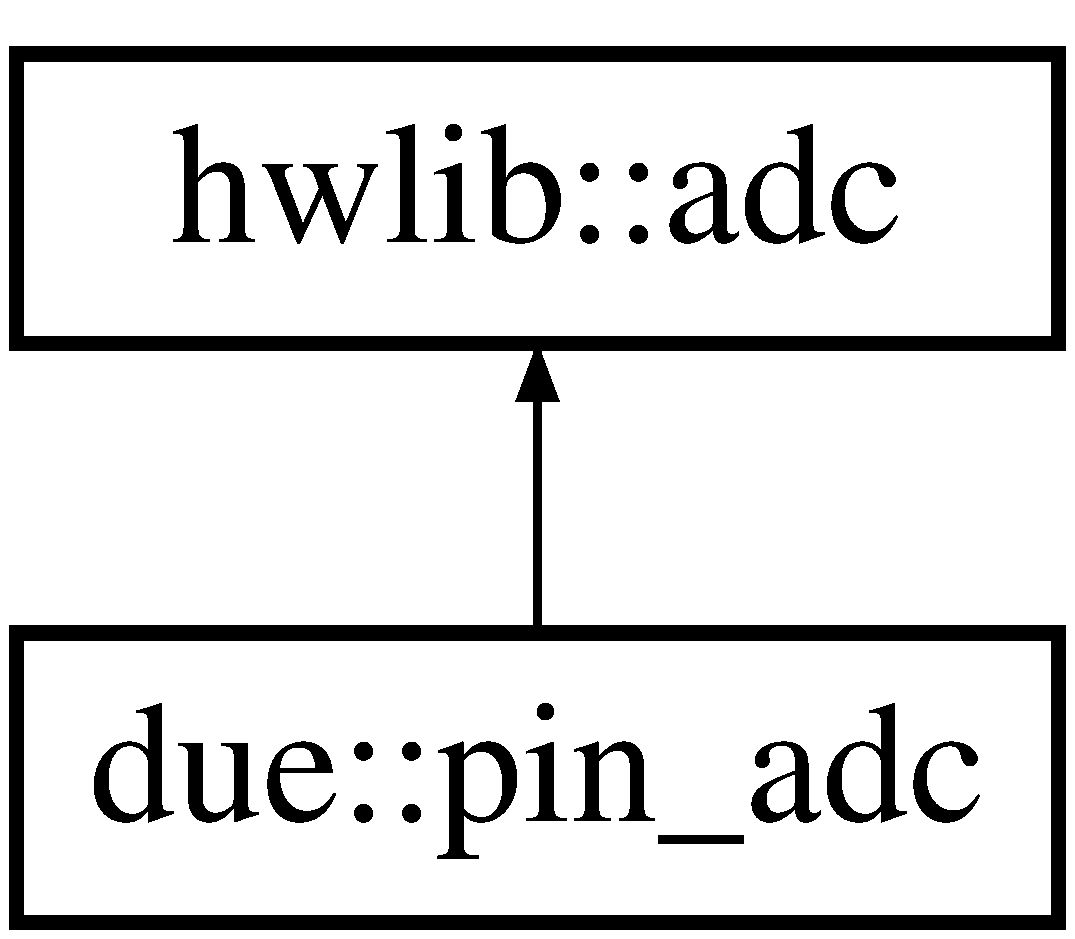
\includegraphics[height=2.000000cm]{classhwlib_1_1adc}
\end{center}
\end{figure}
\subsection*{Public Types}
\begin{DoxyCompactItemize}
\item 
typedef unsigned int \hyperlink{classhwlib_1_1adc_a7ce65f485597a481a518a4b84073605f}{adc\+\_\+value\+\_\+type}\hypertarget{classhwlib_1_1adc_a7ce65f485597a481a518a4b84073605f}{}\label{classhwlib_1_1adc_a7ce65f485597a481a518a4b84073605f}

\begin{DoxyCompactList}\small\item\em the type of the result returned by \hyperlink{classhwlib_1_1adc_a97c3dee32f72a2e7278e01b1a8e924ec}{get()} \end{DoxyCompactList}\end{DoxyCompactItemize}
\subsection*{Public Member Functions}
\begin{DoxyCompactItemize}
\item 
virtual \hyperlink{classhwlib_1_1adc_a7ce65f485597a481a518a4b84073605f}{adc\+\_\+value\+\_\+type} \hyperlink{classhwlib_1_1adc_a97c3dee32f72a2e7278e01b1a8e924ec}{get} ()=0
\begin{DoxyCompactList}\small\item\em do an A/D conversion and return the result \end{DoxyCompactList}\item 
\hyperlink{classhwlib_1_1adc_a7750dfea666ef62fdfb3024cdb66271d}{adc} (int n\+\_\+bits)\hypertarget{classhwlib_1_1adc_a7750dfea666ef62fdfb3024cdb66271d}{}\label{classhwlib_1_1adc_a7750dfea666ef62fdfb3024cdb66271d}

\begin{DoxyCompactList}\small\item\em specify the number of bits \end{DoxyCompactList}\end{DoxyCompactItemize}
\subsection*{Public Attributes}
\begin{DoxyCompactItemize}
\item 
const int \hyperlink{classhwlib_1_1adc_a913b330f5d2a1f12c51e3411fde38217}{adc\+\_\+n\+\_\+bits}\hypertarget{classhwlib_1_1adc_a913b330f5d2a1f12c51e3411fde38217}{}\label{classhwlib_1_1adc_a913b330f5d2a1f12c51e3411fde38217}

\begin{DoxyCompactList}\small\item\em the number of bits in the result returned by \hyperlink{classhwlib_1_1adc_a97c3dee32f72a2e7278e01b1a8e924ec}{get()} \end{DoxyCompactList}\end{DoxyCompactItemize}


\subsection{Detailed Description}
A/D input interface. 

This class abstracts the interface to an A\+DC (Analog to Digital Converter). 

\subsection{Member Function Documentation}
\index{hwlib\+::adc@{hwlib\+::adc}!get@{get}}
\index{get@{get}!hwlib\+::adc@{hwlib\+::adc}}
\subsubsection[{\texorpdfstring{get()=0}{get()=0}}]{\setlength{\rightskip}{0pt plus 5cm}virtual {\bf adc\+\_\+value\+\_\+type} hwlib\+::adc\+::get (
\begin{DoxyParamCaption}
{}
\end{DoxyParamCaption}
)\hspace{0.3cm}{\ttfamily [pure virtual]}}\hypertarget{classhwlib_1_1adc_a97c3dee32f72a2e7278e01b1a8e924ec}{}\label{classhwlib_1_1adc_a97c3dee32f72a2e7278e01b1a8e924ec}


do an A/D conversion and return the result 

This function performs an A/D conversion and returns the result. The lower n\+\_\+bits of the result are the conversion result, the remaining higher bits are 0. 

Implemented in \hyperlink{classdue_1_1pin__adc_a024c090f8d9f0de7a3414d1d3dfe33d9}{due\+::pin\+\_\+adc}.



The documentation for this class was generated from the following file\+:\begin{DoxyCompactItemize}
\item 
\hyperlink{hwlib-adc_8hpp}{hwlib-\/adc.\+hpp}\end{DoxyCompactItemize}

\hypertarget{classhwlib_1_1circle}{}\section{hwlib\+:\+:circle Class Reference}
\label{classhwlib_1_1circle}\index{hwlib\+::circle@{hwlib\+::circle}}


a circle object  




{\ttfamily \#include $<$hwlib-\/graphics.\+hpp$>$}

Inheritance diagram for hwlib\+:\+:circle\+:\begin{figure}[H]
\begin{center}
\leavevmode
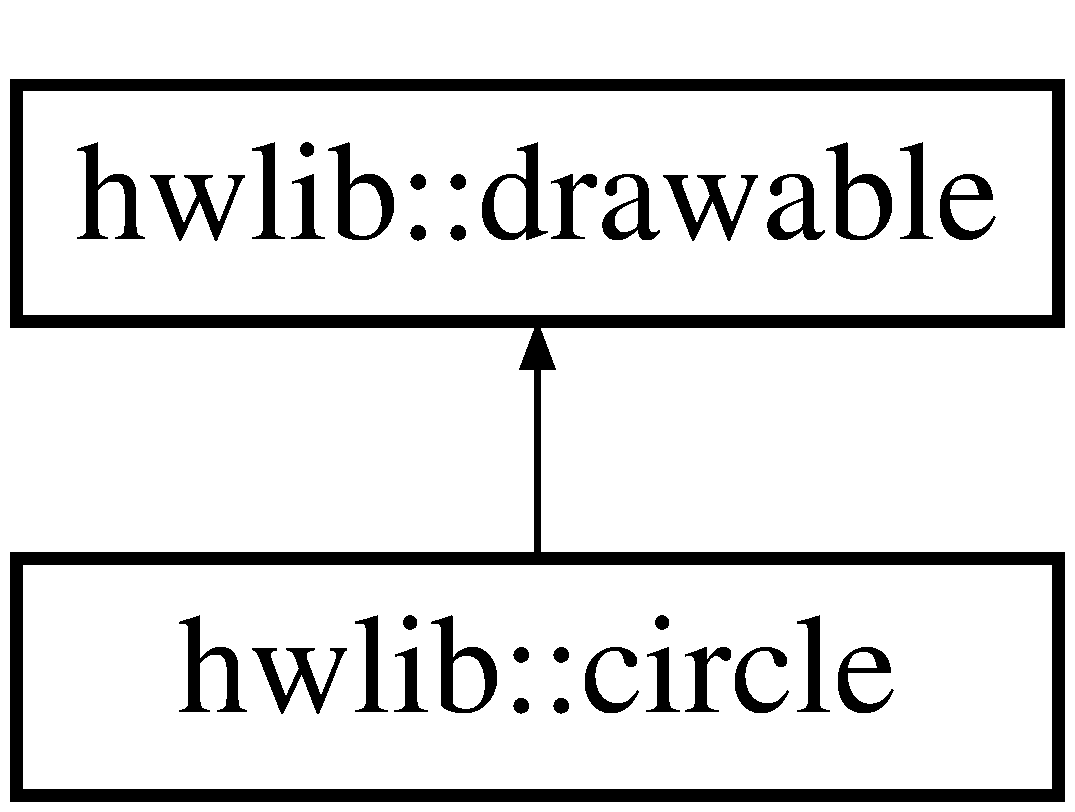
\includegraphics[height=2.000000cm]{classhwlib_1_1circle}
\end{center}
\end{figure}
\subsection*{Public Member Functions}
\begin{DoxyCompactItemize}
\item 
\hyperlink{classhwlib_1_1circle_a072f40759c3083ea2bf1d3b6b7bb91f4}{circle} (\hyperlink{classhwlib_1_1location}{location} \hyperlink{classhwlib_1_1drawable_a6c31bc9303840a4317d3c95250c357ce}{start}, int radius, \hyperlink{classhwlib_1_1color}{color} fg=black, \hyperlink{classhwlib_1_1color}{color} bg=transparent)\hypertarget{classhwlib_1_1circle_a072f40759c3083ea2bf1d3b6b7bb91f4}{}\label{classhwlib_1_1circle_a072f40759c3083ea2bf1d3b6b7bb91f4}

\begin{DoxyCompactList}\small\item\em create a circle object \end{DoxyCompactList}\item 
void \hyperlink{classhwlib_1_1circle_a7a4d6bbd0692b757eee4615a8c5ea9f4}{draw} (\hyperlink{classhwlib_1_1window}{window} \&w) override\hypertarget{classhwlib_1_1circle_a7a4d6bbd0692b757eee4615a8c5ea9f4}{}\label{classhwlib_1_1circle_a7a4d6bbd0692b757eee4615a8c5ea9f4}

\begin{DoxyCompactList}\small\item\em interface to draw the object, you must supply the window \end{DoxyCompactList}\end{DoxyCompactItemize}
\subsection*{Additional Inherited Members}


\subsection{Detailed Description}
a circle object 

The documentation for this class was generated from the following file\+:\begin{DoxyCompactItemize}
\item 
\hyperlink{hwlib-graphics_8hpp}{hwlib-\/graphics.\+hpp}\end{DoxyCompactItemize}

\hypertarget{classhwlib_1_1color}{}\section{hwlib\+:\+:color Class Reference}
\label{classhwlib_1_1color}\index{hwlib\+::color@{hwlib\+::color}}


graphics color  




{\ttfamily \#include $<$hwlib-\/graphics.\+hpp$>$}

\subsection*{Public Member Functions}
\begin{DoxyCompactItemize}
\item 
uint\+\_\+fast32\+\_\+t \hyperlink{classhwlib_1_1color_aefae7dad1c11c2d7b2e3928a3e5bfbc6}{rgb} () const 
\begin{DoxyCompactList}\small\item\em the 3-\/byte R\+GB representation of the color \end{DoxyCompactList}\item 
constexpr \hyperlink{classhwlib_1_1color_ab37154ba89eebb42b162c5c660f40ffa}{color} (int \hyperlink{classhwlib_1_1color_a63b0cdaa1bc446995cc8b8724a2ab866}{red}, int \hyperlink{classhwlib_1_1color_ab87f25b9aba71151e056b570e7304c89}{green}, int \hyperlink{classhwlib_1_1color_a9d57edec257fb2626157befb791a6a96}{blue}, bool transparent=false)
\begin{DoxyCompactList}\small\item\em construct a color from its R\+GB components \end{DoxyCompactList}\item 
constexpr \hyperlink{classhwlib_1_1color_aa8d2263ebf5efe2221171217166a669f}{color} (uint\+\_\+fast32\+\_\+t rgb32=0)
\begin{DoxyCompactList}\small\item\em constructs a color from a three-\/byte integer value \end{DoxyCompactList}\item 
constexpr \hyperlink{classhwlib_1_1color}{color} \hyperlink{classhwlib_1_1color_ab3c5a22a3e8f786082f352d2201886fa}{operator-\/} (void) const \hypertarget{classhwlib_1_1color_ab3c5a22a3e8f786082f352d2201886fa}{}\label{classhwlib_1_1color_ab3c5a22a3e8f786082f352d2201886fa}

\begin{DoxyCompactList}\small\item\em return the negative of a color \end{DoxyCompactList}\item 
constexpr bool \hyperlink{classhwlib_1_1color_a226ee50f35e7668d004593c9bf24a643}{operator==} (const \hyperlink{classhwlib_1_1color}{color} c) const \hypertarget{classhwlib_1_1color_a226ee50f35e7668d004593c9bf24a643}{}\label{classhwlib_1_1color_a226ee50f35e7668d004593c9bf24a643}

\begin{DoxyCompactList}\small\item\em reports whether two colors are equal \end{DoxyCompactList}\item 
constexpr bool \hyperlink{classhwlib_1_1color_a9baf65123cb6bfc8218dd044709d371a}{operator!=} (const \hyperlink{classhwlib_1_1color}{color} c) const \hypertarget{classhwlib_1_1color_a9baf65123cb6bfc8218dd044709d371a}{}\label{classhwlib_1_1color_a9baf65123cb6bfc8218dd044709d371a}

\begin{DoxyCompactList}\small\item\em reports whether two colors are unequal \end{DoxyCompactList}\end{DoxyCompactItemize}
\subsection*{Public Attributes}
\begin{DoxyCompactItemize}
\item 
bool \hyperlink{classhwlib_1_1color_a2bb850a5013f0f4a78b29bd09444fb21}{is\+\_\+transparent}
\begin{DoxyCompactList}\small\item\em the transparency of the color \end{DoxyCompactList}\item 
uint8\+\_\+t \hyperlink{classhwlib_1_1color_a63b0cdaa1bc446995cc8b8724a2ab866}{red}\hypertarget{classhwlib_1_1color_a63b0cdaa1bc446995cc8b8724a2ab866}{}\label{classhwlib_1_1color_a63b0cdaa1bc446995cc8b8724a2ab866}

\begin{DoxyCompactList}\small\item\em the R\+ED attribute (part) of the color \end{DoxyCompactList}\item 
uint8\+\_\+t \hyperlink{classhwlib_1_1color_ab87f25b9aba71151e056b570e7304c89}{green}\hypertarget{classhwlib_1_1color_ab87f25b9aba71151e056b570e7304c89}{}\label{classhwlib_1_1color_ab87f25b9aba71151e056b570e7304c89}

\begin{DoxyCompactList}\small\item\em the G\+R\+E\+EN attribute (part) of the color \end{DoxyCompactList}\item 
uint8\+\_\+t \hyperlink{classhwlib_1_1color_a9d57edec257fb2626157befb791a6a96}{blue}\hypertarget{classhwlib_1_1color_a9d57edec257fb2626157befb791a6a96}{}\label{classhwlib_1_1color_a9d57edec257fb2626157befb791a6a96}

\begin{DoxyCompactList}\small\item\em the B\+L\+UE attribute (part) of the color \end{DoxyCompactList}\end{DoxyCompactItemize}


\subsection{Detailed Description}
graphics color 

This class abstracts a color as used in a graphics window. A color is represented by 3 R\+GB bytes an a transparency flag. 

\subsection{Constructor \& Destructor Documentation}
\index{hwlib\+::color@{hwlib\+::color}!color@{color}}
\index{color@{color}!hwlib\+::color@{hwlib\+::color}}
\subsubsection[{\texorpdfstring{color(int red, int green, int blue, bool transparent=false)}{color(int red, int green, int blue, bool transparent=false)}}]{\setlength{\rightskip}{0pt plus 5cm}constexpr hwlib\+::color\+::color (
\begin{DoxyParamCaption}
\item[{int}]{red, }
\item[{int}]{green, }
\item[{int}]{blue, }
\item[{bool}]{transparent = {\ttfamily false}}
\end{DoxyParamCaption}
)\hspace{0.3cm}{\ttfamily [inline]}}\hypertarget{classhwlib_1_1color_ab37154ba89eebb42b162c5c660f40ffa}{}\label{classhwlib_1_1color_ab37154ba89eebb42b162c5c660f40ffa}


construct a color from its R\+GB components 

The transparency flag can be specified, but better use the transparent constant.

The arguments are integers, but they are clipped to the 0..255 range by the constructor. \index{hwlib\+::color@{hwlib\+::color}!color@{color}}
\index{color@{color}!hwlib\+::color@{hwlib\+::color}}
\subsubsection[{\texorpdfstring{color(uint\+\_\+fast32\+\_\+t rgb32=0)}{color(uint_fast32_t rgb32=0)}}]{\setlength{\rightskip}{0pt plus 5cm}constexpr hwlib\+::color\+::color (
\begin{DoxyParamCaption}
\item[{uint\+\_\+fast32\+\_\+t}]{rgb32 = {\ttfamily 0}}
\end{DoxyParamCaption}
)\hspace{0.3cm}{\ttfamily [inline]}}\hypertarget{classhwlib_1_1color_aa8d2263ebf5efe2221171217166a669f}{}\label{classhwlib_1_1color_aa8d2263ebf5efe2221171217166a669f}


constructs a color from a three-\/byte integer value 

For instance, color( 0x\+F\+F00\+F\+F ) is magenta. 

\subsection{Member Function Documentation}
\index{hwlib\+::color@{hwlib\+::color}!rgb@{rgb}}
\index{rgb@{rgb}!hwlib\+::color@{hwlib\+::color}}
\subsubsection[{\texorpdfstring{rgb() const }{rgb() const }}]{\setlength{\rightskip}{0pt plus 5cm}uint\+\_\+fast32\+\_\+t hwlib\+::color\+::rgb (
\begin{DoxyParamCaption}
{}
\end{DoxyParamCaption}
) const\hspace{0.3cm}{\ttfamily [inline]}}\hypertarget{classhwlib_1_1color_aefae7dad1c11c2d7b2e3928a3e5bfbc6}{}\label{classhwlib_1_1color_aefae7dad1c11c2d7b2e3928a3e5bfbc6}


the 3-\/byte R\+GB representation of the color 

This function returns the R\+GB reprsentation of the color. For a transparent color, the returned value will not be meaningfull. 

\subsection{Member Data Documentation}
\index{hwlib\+::color@{hwlib\+::color}!is\+\_\+transparent@{is\+\_\+transparent}}
\index{is\+\_\+transparent@{is\+\_\+transparent}!hwlib\+::color@{hwlib\+::color}}
\subsubsection[{\texorpdfstring{is\+\_\+transparent}{is_transparent}}]{\setlength{\rightskip}{0pt plus 5cm}bool hwlib\+::color\+::is\+\_\+transparent}\hypertarget{classhwlib_1_1color_a2bb850a5013f0f4a78b29bd09444fb21}{}\label{classhwlib_1_1color_a2bb850a5013f0f4a78b29bd09444fb21}


the transparency of the color 

When a color is tranparent, the read green and blue atrributes are meaningless. 

The documentation for this class was generated from the following file\+:\begin{DoxyCompactItemize}
\item 
\hyperlink{hwlib-graphics_8hpp}{hwlib-\/graphics.\+hpp}\end{DoxyCompactItemize}

\hypertarget{classhwlib_1_1console}{}\section{hwlib\+:\+:console Class Reference}
\label{classhwlib_1_1console}\index{hwlib\+::console@{hwlib\+::console}}


console interface  




{\ttfamily \#include $<$hwlib-\/console.\+hpp$>$}

Inheritance diagram for hwlib\+:\+:console\+:\begin{figure}[H]
\begin{center}
\leavevmode
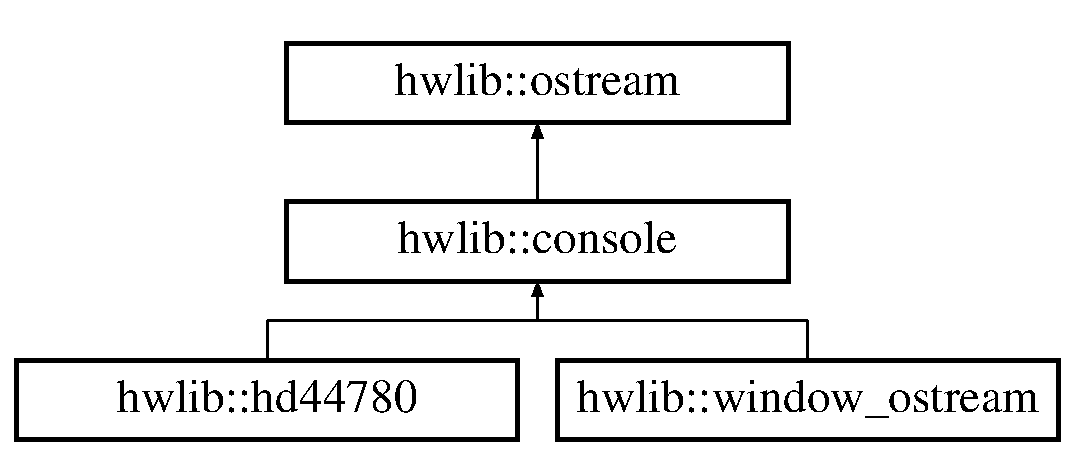
\includegraphics[height=3.000000cm]{classhwlib_1_1console}
\end{center}
\end{figure}
\subsection*{Public Member Functions}
\begin{DoxyCompactItemize}
\item 
\hyperlink{classhwlib_1_1console_a3a5cf41b86ef577bf7c6eea606dfb7f5}{console} (int \hyperlink{classhwlib_1_1console_a5dbe79428aadd15210029a76cb3d255d}{columns}, int \hyperlink{classhwlib_1_1console_a7c5ec25f5c780aaa56702778701ee270}{lines})\hypertarget{classhwlib_1_1console_a3a5cf41b86ef577bf7c6eea606dfb7f5}{}\label{classhwlib_1_1console_a3a5cf41b86ef577bf7c6eea606dfb7f5}

\begin{DoxyCompactList}\small\item\em construct a console from its columns (X size) and lines (Y size) \end{DoxyCompactList}\item 
virtual void \hyperlink{classhwlib_1_1console_a3a9aa37f895584f4b07baadeb0a8827e}{goto\+\_\+xy} (int new\+\_\+x, int new\+\_\+y)\hypertarget{classhwlib_1_1console_a3a9aa37f895584f4b07baadeb0a8827e}{}\label{classhwlib_1_1console_a3a9aa37f895584f4b07baadeb0a8827e}

\begin{DoxyCompactList}\small\item\em put the cursor (write location) at x, y \end{DoxyCompactList}\item 
void \hyperlink{classhwlib_1_1console_ae265a4538a03a68a0ceadcc5fca153f4}{putc} (char c) override\hypertarget{classhwlib_1_1console_ae265a4538a03a68a0ceadcc5fca153f4}{}\label{classhwlib_1_1console_ae265a4538a03a68a0ceadcc5fca153f4}

\begin{DoxyCompactList}\small\item\em write a single character \end{DoxyCompactList}\item 
virtual void \hyperlink{classhwlib_1_1console_a6cc5c79177e0fa54e8fb0e50e30c1d30}{clear} ()
\begin{DoxyCompactList}\small\item\em clear the console \end{DoxyCompactList}\end{DoxyCompactItemize}
\subsection*{Public Attributes}
\begin{DoxyCompactItemize}
\item 
const int \hyperlink{classhwlib_1_1console_a5dbe79428aadd15210029a76cb3d255d}{columns}\hypertarget{classhwlib_1_1console_a5dbe79428aadd15210029a76cb3d255d}{}\label{classhwlib_1_1console_a5dbe79428aadd15210029a76cb3d255d}

\begin{DoxyCompactList}\small\item\em the number of colums in the console \end{DoxyCompactList}\item 
const int \hyperlink{classhwlib_1_1console_a7c5ec25f5c780aaa56702778701ee270}{lines}\hypertarget{classhwlib_1_1console_a7c5ec25f5c780aaa56702778701ee270}{}\label{classhwlib_1_1console_a7c5ec25f5c780aaa56702778701ee270}

\begin{DoxyCompactList}\small\item\em the number of lines (rows) in the console \end{DoxyCompactList}\item 
int \hyperlink{classhwlib_1_1console_a609d3968c3bce1f52481f8a5b7536b42}{x}\hypertarget{classhwlib_1_1console_a609d3968c3bce1f52481f8a5b7536b42}{}\label{classhwlib_1_1console_a609d3968c3bce1f52481f8a5b7536b42}

\begin{DoxyCompactList}\small\item\em the current write column; \end{DoxyCompactList}\item 
int \hyperlink{classhwlib_1_1console_a809dbf940620fe1ef99725f596bf892a}{y}\hypertarget{classhwlib_1_1console_a809dbf940620fe1ef99725f596bf892a}{}\label{classhwlib_1_1console_a809dbf940620fe1ef99725f596bf892a}

\begin{DoxyCompactList}\small\item\em the current write line; \end{DoxyCompactList}\end{DoxyCompactItemize}
\subsection*{Protected Member Functions}
\begin{DoxyCompactItemize}
\item 
virtual void \hyperlink{classhwlib_1_1console_aeced637b949acf507d165eace31bc6ce}{putc\+\_\+implementation} (char c)=0
\begin{DoxyCompactList}\small\item\em the actual writing of a character \end{DoxyCompactList}\item 
virtual void \hyperlink{classhwlib_1_1console_a453717af49292f64a0f51b71f3d02812}{goto\+\_\+xy\+\_\+implementation} (int \hyperlink{classhwlib_1_1console_a609d3968c3bce1f52481f8a5b7536b42}{x}, int \hyperlink{classhwlib_1_1console_a809dbf940620fe1ef99725f596bf892a}{y})
\begin{DoxyCompactList}\small\item\em change the write location to x, y \end{DoxyCompactList}\end{DoxyCompactItemize}
\subsection*{Additional Inherited Members}


\subsection{Detailed Description}
console interface 

This class implements an interface to a character console.

A console is a rectangular windows of (A\+S\+C\+II) characters. A console implements the ostream interface, but it doesn\textquotesingle{}t scroll\+: while the cursor is outside the visible character area (beyond the end of the line, or beyond the number of lines) any character writes will be ignored. Some characters are treated special\+:
\begin{DoxyItemize}
\item \textquotesingle{}\textbackslash{}n\textquotesingle{} puts the cursor at the first position of the next line
\item \textquotesingle{}\textbackslash{}r\textquotesingle{} puts the cursor at the start of the current line
\item \textquotesingle{}\textbackslash{}f\textquotesingle{} puts the cursor at the top-\/left position and clears the console
\item \textquotesingle{}\textbackslash{}txxyy\textquotesingle{} puts the cursor at the position (xx,yy)
\end{DoxyItemize}

The x and y coordinates are 0-\/origin and count to the right and down. In other words, the top-\/left character position is (0,0), and the bottom right character position is (rows -\/ 1, columns -\/ 1).

 

\subsection{Member Function Documentation}
\index{hwlib\+::console@{hwlib\+::console}!clear@{clear}}
\index{clear@{clear}!hwlib\+::console@{hwlib\+::console}}
\subsubsection[{\texorpdfstring{clear()}{clear()}}]{\setlength{\rightskip}{0pt plus 5cm}virtual void hwlib\+::console\+::clear (
\begin{DoxyParamCaption}
{}
\end{DoxyParamCaption}
)\hspace{0.3cm}{\ttfamily [inline]}, {\ttfamily [virtual]}}\hypertarget{classhwlib_1_1console_a6cc5c79177e0fa54e8fb0e50e30c1d30}{}\label{classhwlib_1_1console_a6cc5c79177e0fa54e8fb0e50e30c1d30}


clear the console 

This function clears the console and puts the cursor at (0,0). The default implementation does this by writing spaces to all locations. A concrete implementation might provide a better (faster) way. 

Reimplemented in \hyperlink{classhwlib_1_1hd44780_a45d4a84c9da66fa350270df482c6e58f}{hwlib\+::hd44780}.

\index{hwlib\+::console@{hwlib\+::console}!goto\+\_\+xy\+\_\+implementation@{goto\+\_\+xy\+\_\+implementation}}
\index{goto\+\_\+xy\+\_\+implementation@{goto\+\_\+xy\+\_\+implementation}!hwlib\+::console@{hwlib\+::console}}
\subsubsection[{\texorpdfstring{goto\+\_\+xy\+\_\+implementation(int x, int y)}{goto_xy_implementation(int x, int y)}}]{\setlength{\rightskip}{0pt plus 5cm}virtual void hwlib\+::console\+::goto\+\_\+xy\+\_\+implementation (
\begin{DoxyParamCaption}
\item[{int}]{x, }
\item[{int}]{y}
\end{DoxyParamCaption}
)\hspace{0.3cm}{\ttfamily [inline]}, {\ttfamily [protected]}, {\ttfamily [virtual]}}\hypertarget{classhwlib_1_1console_a453717af49292f64a0f51b71f3d02812}{}\label{classhwlib_1_1console_a453717af49292f64a0f51b71f3d02812}


change the write location to x, y 

This function is called when the write location is changed {\itshape except} when it is changed to the next x position by a call to putc\+\_\+implementation.

The default implementation does nothing. \index{hwlib\+::console@{hwlib\+::console}!putc\+\_\+implementation@{putc\+\_\+implementation}}
\index{putc\+\_\+implementation@{putc\+\_\+implementation}!hwlib\+::console@{hwlib\+::console}}
\subsubsection[{\texorpdfstring{putc\+\_\+implementation(char c)=0}{putc_implementation(char c)=0}}]{\setlength{\rightskip}{0pt plus 5cm}virtual void hwlib\+::console\+::putc\+\_\+implementation (
\begin{DoxyParamCaption}
\item[{char}]{c}
\end{DoxyParamCaption}
)\hspace{0.3cm}{\ttfamily [protected]}, {\ttfamily [pure virtual]}}\hypertarget{classhwlib_1_1console_aeced637b949acf507d165eace31bc6ce}{}\label{classhwlib_1_1console_aeced637b949acf507d165eace31bc6ce}


the actual writing of a character 

When this function is called, the the current cursor is guaranteed to be within the console, and the character is not one of the special characters (\textbackslash{}n, \textbackslash{}r, \textbackslash{}c) 

The documentation for this class was generated from the following file\+:\begin{DoxyCompactItemize}
\item 
\hyperlink{hwlib-console_8hpp}{hwlib-\/console.\+hpp}\end{DoxyCompactItemize}

\hypertarget{classdue_1_1d2__36k_hz}{}\section{due\+:\+:d2\+\_\+36k\+Hz Class Reference}
\label{classdue_1_1d2__36k_hz}\index{due\+::d2\+\_\+36k\+Hz@{due\+::d2\+\_\+36k\+Hz}}


{\ttfamily \#include $<$hwlib-\/due.\+hpp$>$}

Inheritance diagram for due\+:\+:d2\+\_\+36k\+Hz\+:\begin{figure}[H]
\begin{center}
\leavevmode
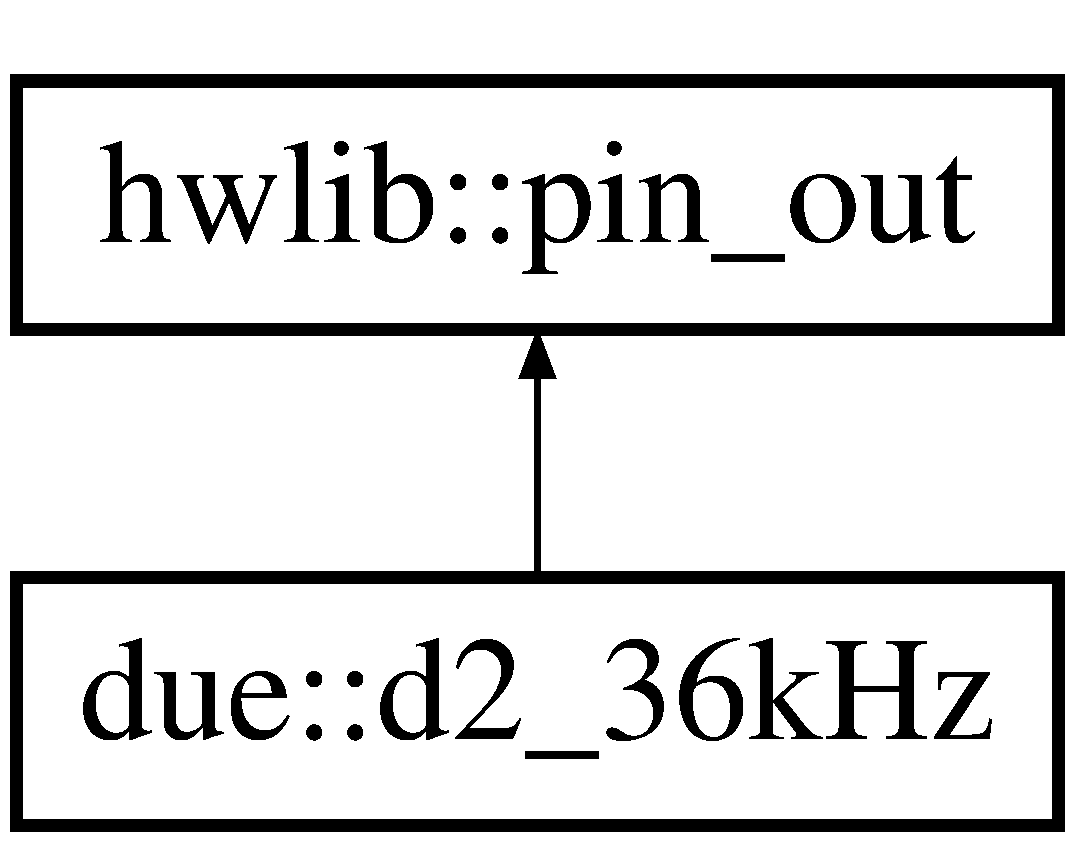
\includegraphics[height=2.000000cm]{classdue_1_1d2__36k_hz}
\end{center}
\end{figure}
\subsection*{Public Member Functions}
\begin{DoxyCompactItemize}
\item 
\hyperlink{classdue_1_1d2__36k_hz_a9172955a5667b99410897e2cabed24d2}{d2\+\_\+36k\+Hz} ()\hypertarget{classdue_1_1d2__36k_hz_a9172955a5667b99410897e2cabed24d2}{}\label{classdue_1_1d2__36k_hz_a9172955a5667b99410897e2cabed24d2}

\begin{DoxyCompactList}\small\item\em create the 36k\+Hz output \end{DoxyCompactList}\item 
void \hyperlink{classdue_1_1d2__36k_hz_abdb0b8ee44017ecfaf37fcbf9e0ba126}{set} (bool b) override
\begin{DoxyCompactList}\small\item\em enable or disable the 36 k\+Hz output \end{DoxyCompactList}\end{DoxyCompactItemize}


\subsection{Detailed Description}
36k\+Hz output on pin chip P\+B25 = Arduino D2

This class provides a 36 k\+Hz output on chip pin P\+B25 (Arduino pin D2) that can be enabled or disabled by calling set( 1 ) resp. set( 0 ). 

\subsection{Member Function Documentation}
\index{due\+::d2\+\_\+36k\+Hz@{due\+::d2\+\_\+36k\+Hz}!set@{set}}
\index{set@{set}!due\+::d2\+\_\+36k\+Hz@{due\+::d2\+\_\+36k\+Hz}}
\subsubsection[{\texorpdfstring{set(bool b) override}{set(bool b) override}}]{\setlength{\rightskip}{0pt plus 5cm}void due\+::d2\+\_\+36k\+Hz\+::set (
\begin{DoxyParamCaption}
\item[{bool}]{b}
\end{DoxyParamCaption}
)\hspace{0.3cm}{\ttfamily [inline]}, {\ttfamily [override]}, {\ttfamily [virtual]}}\hypertarget{classdue_1_1d2__36k_hz_abdb0b8ee44017ecfaf37fcbf9e0ba126}{}\label{classdue_1_1d2__36k_hz_abdb0b8ee44017ecfaf37fcbf9e0ba126}


enable or disable the 36 k\+Hz output 

Calling set( 1 ) enables the 36 k\+Hz output, calling set( 0 ) disables the output and makes the output low. 

Implements \hyperlink{classhwlib_1_1pin__out_af5c3a533f1a00ba973e37e60fb8c08c6}{hwlib\+::pin\+\_\+out}.



The documentation for this class was generated from the following file\+:\begin{DoxyCompactItemize}
\item 
\hyperlink{hwlib-due_8hpp}{hwlib-\/due.\+hpp}\end{DoxyCompactItemize}

\hypertarget{classhwlib_1_1dac}{}\section{hwlib\+:\+:dac Class Reference}
\label{classhwlib_1_1dac}\index{hwlib\+::dac@{hwlib\+::dac}}


D/A output interface.  




{\ttfamily \#include $<$hwlib-\/dac.\+hpp$>$}

\subsection*{Public Types}
\begin{DoxyCompactItemize}
\item 
typedef unsigned int \hyperlink{classhwlib_1_1dac_a63d1c11b81be9215e94eb81981045a22}{dac\+\_\+value\+\_\+type}\hypertarget{classhwlib_1_1dac_a63d1c11b81be9215e94eb81981045a22}{}\label{classhwlib_1_1dac_a63d1c11b81be9215e94eb81981045a22}

\begin{DoxyCompactList}\small\item\em the type of the result returned by get() \end{DoxyCompactList}\end{DoxyCompactItemize}
\subsection*{Public Member Functions}
\begin{DoxyCompactItemize}
\item 
virtual void \hyperlink{classhwlib_1_1dac_aba799313f06200f44c5146643abe4e08}{set} (\hyperlink{classhwlib_1_1dac_a63d1c11b81be9215e94eb81981045a22}{dac\+\_\+value\+\_\+type} x)=0
\begin{DoxyCompactList}\small\item\em write a value to the D/A output \end{DoxyCompactList}\item 
\hyperlink{classhwlib_1_1dac_a09b329cd33da005b6a55bafafba36e62}{dac} (int n\+\_\+bits)\hypertarget{classhwlib_1_1dac_a09b329cd33da005b6a55bafafba36e62}{}\label{classhwlib_1_1dac_a09b329cd33da005b6a55bafafba36e62}

\begin{DoxyCompactList}\small\item\em specify the number of bits \end{DoxyCompactList}\end{DoxyCompactItemize}
\subsection*{Public Attributes}
\begin{DoxyCompactItemize}
\item 
const int \hyperlink{classhwlib_1_1dac_a70e7117d7f09c795b3dba20290add539}{dac\+\_\+n\+\_\+bits}\hypertarget{classhwlib_1_1dac_a70e7117d7f09c795b3dba20290add539}{}\label{classhwlib_1_1dac_a70e7117d7f09c795b3dba20290add539}

\begin{DoxyCompactList}\small\item\em the number of bits in the result returned by get() \end{DoxyCompactList}\end{DoxyCompactItemize}


\subsection{Detailed Description}
D/A output interface. 

This class abstracts the interface to a D\+AC (Digital to Analog Converter). 

\subsection{Member Function Documentation}
\index{hwlib\+::dac@{hwlib\+::dac}!set@{set}}
\index{set@{set}!hwlib\+::dac@{hwlib\+::dac}}
\subsubsection[{\texorpdfstring{set(dac\+\_\+value\+\_\+type x)=0}{set(dac_value_type x)=0}}]{\setlength{\rightskip}{0pt plus 5cm}virtual void hwlib\+::dac\+::set (
\begin{DoxyParamCaption}
\item[{{\bf dac\+\_\+value\+\_\+type}}]{x}
\end{DoxyParamCaption}
)\hspace{0.3cm}{\ttfamily [pure virtual]}}\hypertarget{classhwlib_1_1dac_aba799313f06200f44c5146643abe4e08}{}\label{classhwlib_1_1dac_aba799313f06200f44c5146643abe4e08}


write a value to the D/A output 

This writes a digital value to the D/A converter, which causes the corresponding analog value to appear on the output pin. 

The documentation for this class was generated from the following file\+:\begin{DoxyCompactItemize}
\item 
\hyperlink{hwlib-dac_8hpp}{hwlib-\/dac.\+hpp}\end{DoxyCompactItemize}

\hypertarget{classhwlib_1_1drawable}{}\section{hwlib\+:\+:drawable Class Reference}
\label{classhwlib_1_1drawable}\index{hwlib\+::drawable@{hwlib\+::drawable}}


interface to an drawable object  




{\ttfamily \#include $<$hwlib-\/graphics.\+hpp$>$}

Inheritance diagram for hwlib\+:\+:drawable\+:\begin{figure}[H]
\begin{center}
\leavevmode
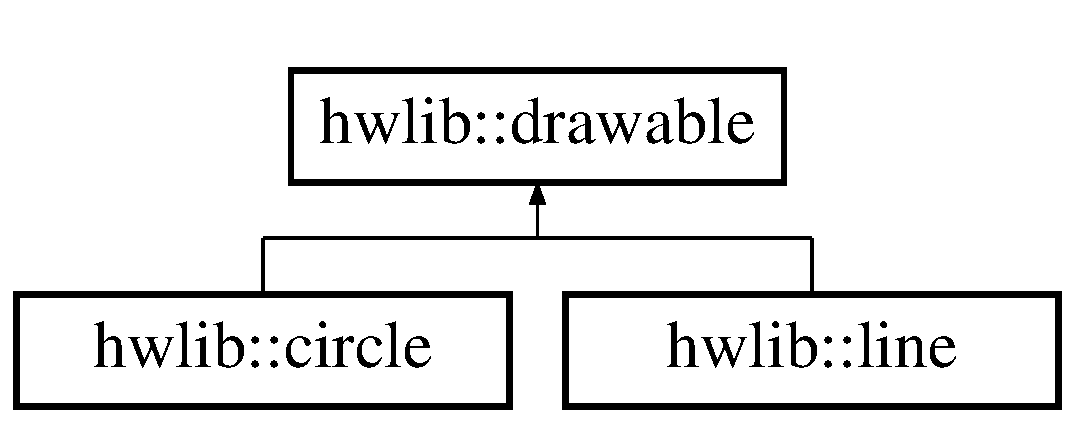
\includegraphics[height=2.000000cm]{classhwlib_1_1drawable}
\end{center}
\end{figure}
\subsection*{Public Member Functions}
\begin{DoxyCompactItemize}
\item 
\hyperlink{classhwlib_1_1drawable_a48f84ea64249fe67f726e9631d149d66}{drawable} (\hyperlink{classhwlib_1_1location}{location} \hyperlink{classhwlib_1_1drawable_a6c31bc9303840a4317d3c95250c357ce}{start})\hypertarget{classhwlib_1_1drawable_a48f84ea64249fe67f726e9631d149d66}{}\label{classhwlib_1_1drawable_a48f84ea64249fe67f726e9631d149d66}

\begin{DoxyCompactList}\small\item\em create a drawable object by bsupplying its (initial) location \end{DoxyCompactList}\item 
virtual void \hyperlink{classhwlib_1_1drawable_ac9ea0de52a14d9024cb34110f794ac28}{draw} (\hyperlink{classhwlib_1_1window}{window} \&w)=0\hypertarget{classhwlib_1_1drawable_ac9ea0de52a14d9024cb34110f794ac28}{}\label{classhwlib_1_1drawable_ac9ea0de52a14d9024cb34110f794ac28}

\begin{DoxyCompactList}\small\item\em interface to draw the object, you must supply the window \end{DoxyCompactList}\end{DoxyCompactItemize}
\subsection*{Public Attributes}
\begin{DoxyCompactItemize}
\item 
\hyperlink{classhwlib_1_1location}{location} \hyperlink{classhwlib_1_1drawable_a6c31bc9303840a4317d3c95250c357ce}{start}\hypertarget{classhwlib_1_1drawable_a6c31bc9303840a4317d3c95250c357ce}{}\label{classhwlib_1_1drawable_a6c31bc9303840a4317d3c95250c357ce}

\begin{DoxyCompactList}\small\item\em the location where the object is drawn \end{DoxyCompactList}\end{DoxyCompactItemize}


\subsection{Detailed Description}
interface to an drawable object 

The documentation for this class was generated from the following file\+:\begin{DoxyCompactItemize}
\item 
\hyperlink{hwlib-graphics_8hpp}{hwlib-\/graphics.\+hpp}\end{DoxyCompactItemize}

\hypertarget{classhwlib_1_1font}{}\section{hwlib\+:\+:font Class Reference}
\label{classhwlib_1_1font}\index{hwlib\+::font@{hwlib\+::font}}


a font  




{\ttfamily \#include $<$hwlib-\/graphics.\+hpp$>$}

Inheritance diagram for hwlib\+:\+:font\+:\begin{figure}[H]
\begin{center}
\leavevmode
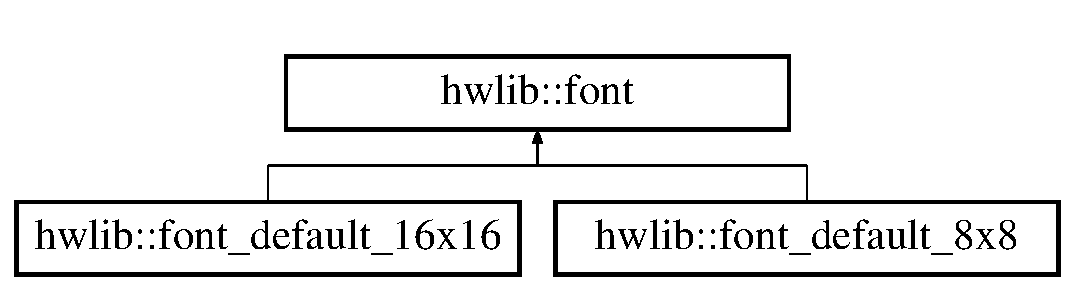
\includegraphics[height=2.000000cm]{classhwlib_1_1font}
\end{center}
\end{figure}
\subsection*{Public Member Functions}
\begin{DoxyCompactItemize}
\item 
virtual const \hyperlink{classhwlib_1_1image}{image} \& \hyperlink{classhwlib_1_1font_ab292f5c14db5727c2ef67cfa8df4e88d}{operator\mbox{[}$\,$\mbox{]}} (char c) const  =0
\begin{DoxyCompactList}\small\item\em get image for a character \end{DoxyCompactList}\end{DoxyCompactItemize}


\subsection{Detailed Description}
a font 

A font provides an image for each supported character 

\subsection{Member Function Documentation}
\index{hwlib\+::font@{hwlib\+::font}!operator\mbox{[}$\,$\mbox{]}@{operator[]}}
\index{operator\mbox{[}$\,$\mbox{]}@{operator[]}!hwlib\+::font@{hwlib\+::font}}
\subsubsection[{\texorpdfstring{operator[](char c) const  =0}{operator[](char c) const  =0}}]{\setlength{\rightskip}{0pt plus 5cm}virtual const {\bf image}\& hwlib\+::font\+::operator\mbox{[}$\,$\mbox{]} (
\begin{DoxyParamCaption}
\item[{char}]{c}
\end{DoxyParamCaption}
) const\hspace{0.3cm}{\ttfamily [pure virtual]}}\hypertarget{classhwlib_1_1font_ab292f5c14db5727c2ef67cfa8df4e88d}{}\label{classhwlib_1_1font_ab292f5c14db5727c2ef67cfa8df4e88d}


get image for a character 

This function returns the image for the specified character. 

Implemented in \hyperlink{classhwlib_1_1font__default__16x16_a081cf441b349ffd7090f7481c86d54f3}{hwlib\+::font\+\_\+default\+\_\+16x16}, and \hyperlink{classhwlib_1_1font__default__8x8_ad52322d744ff9758015633585c8be0ea}{hwlib\+::font\+\_\+default\+\_\+8x8}.



The documentation for this class was generated from the following file\+:\begin{DoxyCompactItemize}
\item 
\hyperlink{hwlib-graphics_8hpp}{hwlib-\/graphics.\+hpp}\end{DoxyCompactItemize}

\hypertarget{classhwlib_1_1font__default__16x16}{}\section{hwlib\+:\+:font\+\_\+default\+\_\+16x16 Class Reference}
\label{classhwlib_1_1font__default__16x16}\index{hwlib\+::font\+\_\+default\+\_\+16x16@{hwlib\+::font\+\_\+default\+\_\+16x16}}
Inheritance diagram for hwlib\+:\+:font\+\_\+default\+\_\+16x16\+:\begin{figure}[H]
\begin{center}
\leavevmode
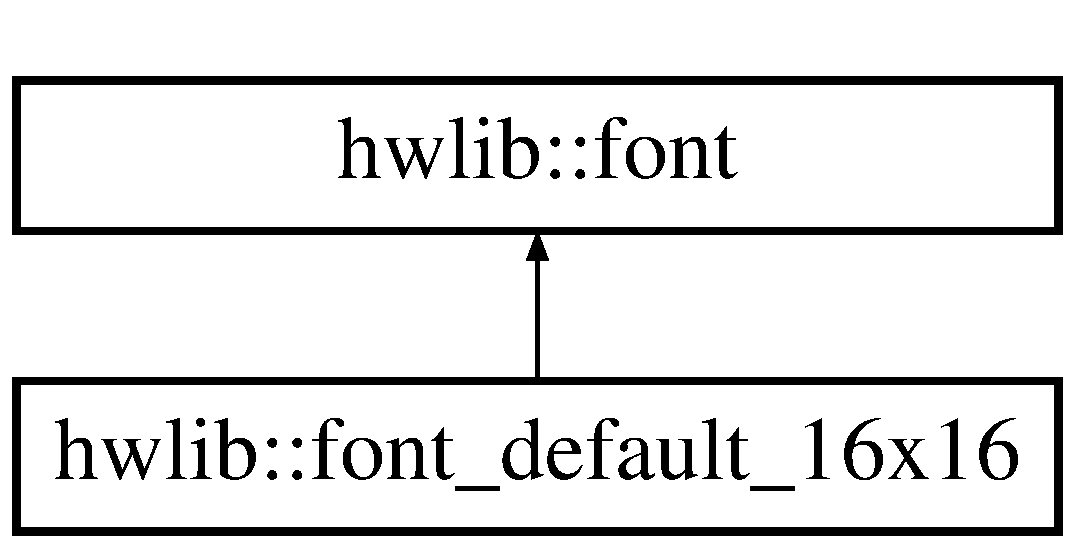
\includegraphics[height=2.000000cm]{classhwlib_1_1font__default__16x16}
\end{center}
\end{figure}
\subsection*{Public Member Functions}
\begin{DoxyCompactItemize}
\item 
const \hyperlink{classhwlib_1_1image}{image} \& \hyperlink{classhwlib_1_1font__default__16x16_a081cf441b349ffd7090f7481c86d54f3}{operator\mbox{[}$\,$\mbox{]}} (char c) const  override
\begin{DoxyCompactList}\small\item\em get image for a character \end{DoxyCompactList}\end{DoxyCompactItemize}


\subsection{Member Function Documentation}
\index{hwlib\+::font\+\_\+default\+\_\+16x16@{hwlib\+::font\+\_\+default\+\_\+16x16}!operator\mbox{[}$\,$\mbox{]}@{operator[]}}
\index{operator\mbox{[}$\,$\mbox{]}@{operator[]}!hwlib\+::font\+\_\+default\+\_\+16x16@{hwlib\+::font\+\_\+default\+\_\+16x16}}
\subsubsection[{\texorpdfstring{operator[](char c) const  override}{operator[](char c) const  override}}]{\setlength{\rightskip}{0pt plus 5cm}const {\bf image}\& hwlib\+::font\+\_\+default\+\_\+16x16\+::operator\mbox{[}$\,$\mbox{]} (
\begin{DoxyParamCaption}
\item[{char}]{c}
\end{DoxyParamCaption}
) const\hspace{0.3cm}{\ttfamily [inline]}, {\ttfamily [override]}, {\ttfamily [virtual]}}\hypertarget{classhwlib_1_1font__default__16x16_a081cf441b349ffd7090f7481c86d54f3}{}\label{classhwlib_1_1font__default__16x16_a081cf441b349ffd7090f7481c86d54f3}


get image for a character 

This function returns the image for the specified character. 

Implements \hyperlink{classhwlib_1_1font_ab292f5c14db5727c2ef67cfa8df4e88d}{hwlib\+::font}.



The documentation for this class was generated from the following file\+:\begin{DoxyCompactItemize}
\item 
\hyperlink{hwlib-font-default-16x16_8hpp}{hwlib-\/font-\/default-\/16x16.\+hpp}\end{DoxyCompactItemize}

\hypertarget{classhwlib_1_1font__default__8x8}{}\section{hwlib\+:\+:font\+\_\+default\+\_\+8x8 Class Reference}
\label{classhwlib_1_1font__default__8x8}\index{hwlib\+::font\+\_\+default\+\_\+8x8@{hwlib\+::font\+\_\+default\+\_\+8x8}}
Inheritance diagram for hwlib\+:\+:font\+\_\+default\+\_\+8x8\+:\begin{figure}[H]
\begin{center}
\leavevmode
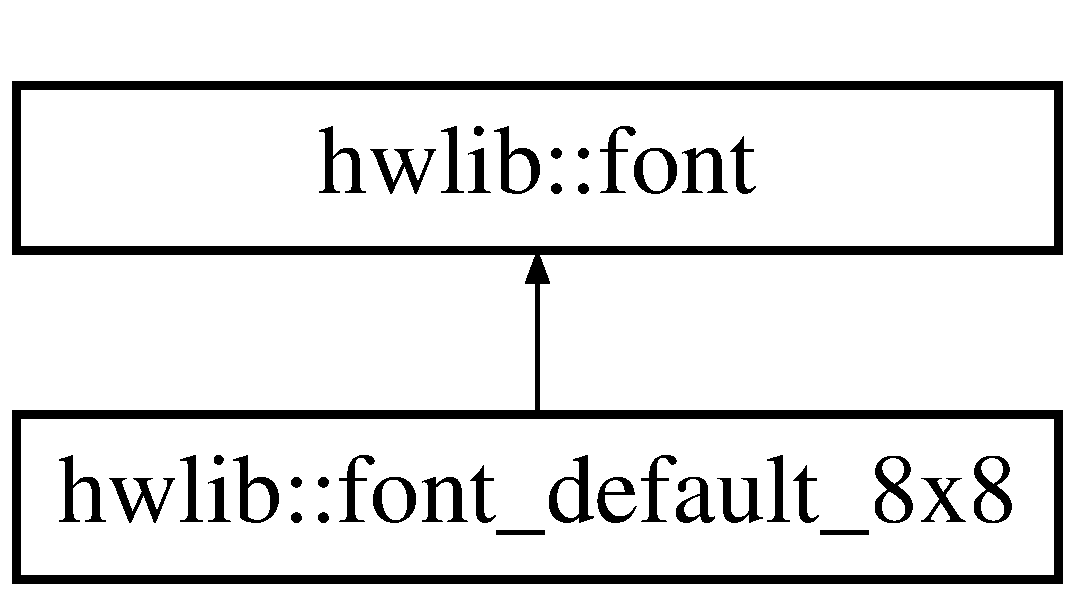
\includegraphics[height=2.000000cm]{classhwlib_1_1font__default__8x8}
\end{center}
\end{figure}
\subsection*{Public Member Functions}
\begin{DoxyCompactItemize}
\item 
constexpr const \hyperlink{classhwlib_1_1image}{image} \& \hyperlink{classhwlib_1_1font__default__8x8_ad52322d744ff9758015633585c8be0ea}{operator\mbox{[}$\,$\mbox{]}} (char c) const  override
\begin{DoxyCompactList}\small\item\em get image for a character \end{DoxyCompactList}\end{DoxyCompactItemize}


\subsection{Member Function Documentation}
\index{hwlib\+::font\+\_\+default\+\_\+8x8@{hwlib\+::font\+\_\+default\+\_\+8x8}!operator\mbox{[}$\,$\mbox{]}@{operator[]}}
\index{operator\mbox{[}$\,$\mbox{]}@{operator[]}!hwlib\+::font\+\_\+default\+\_\+8x8@{hwlib\+::font\+\_\+default\+\_\+8x8}}
\subsubsection[{\texorpdfstring{operator[](char c) const  override}{operator[](char c) const  override}}]{\setlength{\rightskip}{0pt plus 5cm}constexpr const {\bf image}\& hwlib\+::font\+\_\+default\+\_\+8x8\+::operator\mbox{[}$\,$\mbox{]} (
\begin{DoxyParamCaption}
\item[{char}]{c}
\end{DoxyParamCaption}
) const\hspace{0.3cm}{\ttfamily [inline]}, {\ttfamily [override]}, {\ttfamily [virtual]}}\hypertarget{classhwlib_1_1font__default__8x8_ad52322d744ff9758015633585c8be0ea}{}\label{classhwlib_1_1font__default__8x8_ad52322d744ff9758015633585c8be0ea}


get image for a character 

This function returns the image for the specified character. 

Implements \hyperlink{classhwlib_1_1font_ab292f5c14db5727c2ef67cfa8df4e88d}{hwlib\+::font}.



The documentation for this class was generated from the following file\+:\begin{DoxyCompactItemize}
\item 
\hyperlink{hwlib-font-default-8x8_8hpp}{hwlib-\/font-\/default-\/8x8.\+hpp}\end{DoxyCompactItemize}

\hypertarget{classhwlib_1_1glcd__5510}{}\section{hwlib\+:\+:glcd\+\_\+5510 Class Reference}
\label{classhwlib_1_1glcd__5510}\index{hwlib\+::glcd\+\_\+5510@{hwlib\+::glcd\+\_\+5510}}


Nokia 5510 B/W graphics L\+CD library.  




{\ttfamily \#include $<$hwlib-\/glcd-\/5510.\+hpp$>$}

Inheritance diagram for hwlib\+:\+:glcd\+\_\+5510\+:\begin{figure}[H]
\begin{center}
\leavevmode
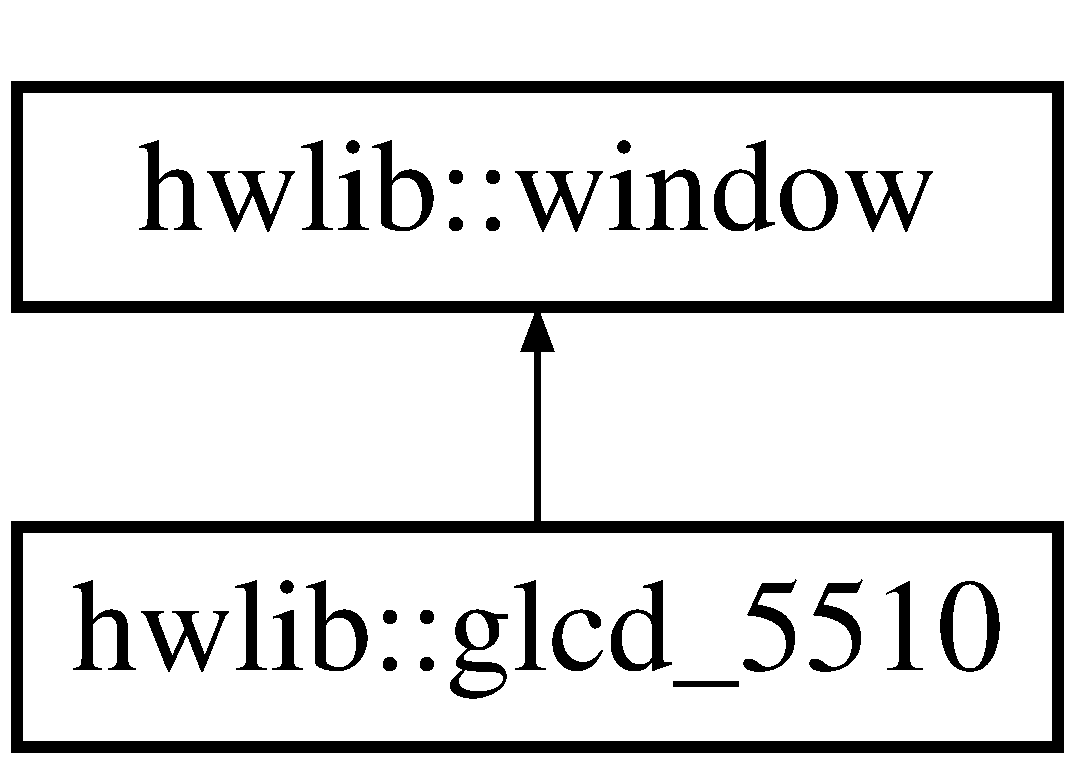
\includegraphics[height=2.000000cm]{classhwlib_1_1glcd__5510}
\end{center}
\end{figure}
\subsection*{Public Member Functions}
\begin{DoxyCompactItemize}
\item 
\hyperlink{classhwlib_1_1glcd__5510_a689cb8a2f60f76f087b83626b2ca931a}{glcd\+\_\+5510} (\hyperlink{classhwlib_1_1pin__out}{pin\+\_\+out} \&sce, \hyperlink{classhwlib_1_1pin__out}{pin\+\_\+out} \&res, \hyperlink{classhwlib_1_1pin__out}{pin\+\_\+out} \&dc, \hyperlink{classhwlib_1_1pin__out}{pin\+\_\+out} \&sdin, \hyperlink{classhwlib_1_1pin__out}{pin\+\_\+out} \&sclk)
\begin{DoxyCompactList}\small\item\em construct the L\+CD \end{DoxyCompactList}\item 
void \hyperlink{classhwlib_1_1glcd__5510_a533b2663e151bee909543d0038b2cb4d}{clear} () override
\begin{DoxyCompactList}\small\item\em clear the window \end{DoxyCompactList}\end{DoxyCompactItemize}
\subsection*{Additional Inherited Members}


\subsection{Detailed Description}
Nokia 5510 B/W graphics L\+CD library. 

This class implements an interface to the type of L\+CD that was used in older Nokia telephones. It is a 84 columns x 48 lines black-\/and-\/white L\+CD.

This type of L\+CD is cheap and available from lots of sources, but the quality is often abominable.

 

\subsection{Constructor \& Destructor Documentation}
\index{hwlib\+::glcd\+\_\+5510@{hwlib\+::glcd\+\_\+5510}!glcd\+\_\+5510@{glcd\+\_\+5510}}
\index{glcd\+\_\+5510@{glcd\+\_\+5510}!hwlib\+::glcd\+\_\+5510@{hwlib\+::glcd\+\_\+5510}}
\subsubsection[{\texorpdfstring{glcd\+\_\+5510(pin\+\_\+out \&sce, pin\+\_\+out \&res, pin\+\_\+out \&dc, pin\+\_\+out \&sdin, pin\+\_\+out \&sclk)}{glcd_5510(pin_out &sce, pin_out &res, pin_out &dc, pin_out &sdin, pin_out &sclk)}}]{\setlength{\rightskip}{0pt plus 5cm}hwlib\+::glcd\+\_\+5510\+::glcd\+\_\+5510 (
\begin{DoxyParamCaption}
\item[{{\bf pin\+\_\+out} \&}]{sce, }
\item[{{\bf pin\+\_\+out} \&}]{res, }
\item[{{\bf pin\+\_\+out} \&}]{dc, }
\item[{{\bf pin\+\_\+out} \&}]{sdin, }
\item[{{\bf pin\+\_\+out} \&}]{sclk}
\end{DoxyParamCaption}
)\hspace{0.3cm}{\ttfamily [inline]}}\hypertarget{classhwlib_1_1glcd__5510_a689cb8a2f60f76f087b83626b2ca931a}{}\label{classhwlib_1_1glcd__5510_a689cb8a2f60f76f087b83626b2ca931a}


construct the L\+CD 

This function creates a 5510 L\+CD from its interface pins. 

\subsection{Member Function Documentation}
\index{hwlib\+::glcd\+\_\+5510@{hwlib\+::glcd\+\_\+5510}!clear@{clear}}
\index{clear@{clear}!hwlib\+::glcd\+\_\+5510@{hwlib\+::glcd\+\_\+5510}}
\subsubsection[{\texorpdfstring{clear() override}{clear() override}}]{\setlength{\rightskip}{0pt plus 5cm}void hwlib\+::glcd\+\_\+5510\+::clear (
\begin{DoxyParamCaption}
{}
\end{DoxyParamCaption}
)\hspace{0.3cm}{\ttfamily [inline]}, {\ttfamily [override]}, {\ttfamily [virtual]}}\hypertarget{classhwlib_1_1glcd__5510_a533b2663e151bee909543d0038b2cb4d}{}\label{classhwlib_1_1glcd__5510_a533b2663e151bee909543d0038b2cb4d}


clear the window 

This function clears the windows by writing the background color to all pixels. The default implementation writes to all pixels in sequence. A concrete window can probably provide a faster implementation. 

Reimplemented from \hyperlink{classhwlib_1_1window_a5e781163353ce26cb4dc5b2cbe40ad05}{hwlib\+::window}.



The documentation for this class was generated from the following file\+:\begin{DoxyCompactItemize}
\item 
\hyperlink{hwlib-glcd-5510_8hpp}{hwlib-\/glcd-\/5510.\+hpp}\end{DoxyCompactItemize}

\hypertarget{classhwlib_1_1glcd__oled}{}\section{hwlib\+:\+:glcd\+\_\+oled Class Reference}
\label{classhwlib_1_1glcd__oled}\index{hwlib\+::glcd\+\_\+oled@{hwlib\+::glcd\+\_\+oled}}


Oled B/W graphics L\+CD.  




{\ttfamily \#include $<$hwlib-\/glcd-\/oled.\+hpp$>$}

Inheritance diagram for hwlib\+:\+:glcd\+\_\+oled\+:\begin{figure}[H]
\begin{center}
\leavevmode
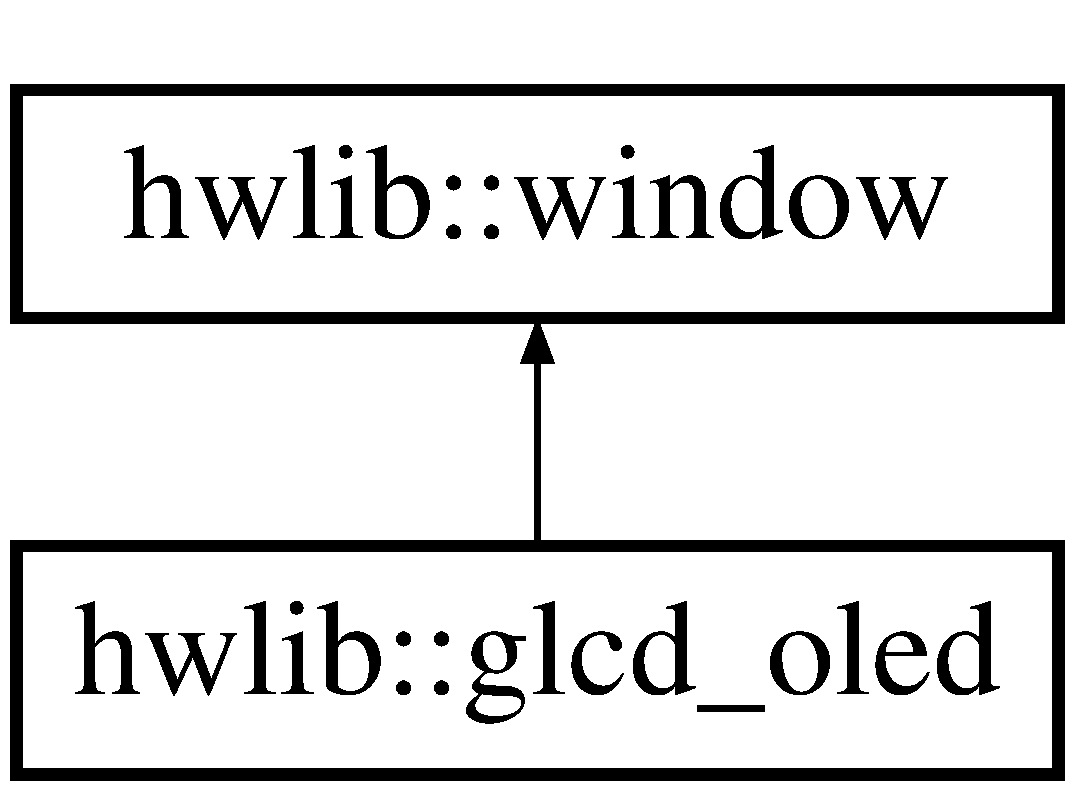
\includegraphics[height=2.000000cm]{classhwlib_1_1glcd__oled}
\end{center}
\end{figure}
\subsection*{Public Member Functions}
\begin{DoxyCompactItemize}
\item 
{\bfseries glcd\+\_\+oled} (\hyperlink{classhwlib_1_1i2c__bus}{i2c\+\_\+bus} \&bus, \hyperlink{hwlib-defines_8hpp_a54998f25522db04b7b797b0fcc9eb3d5}{fast\+\_\+byte} address=0x3\+C)\hypertarget{classhwlib_1_1glcd__oled_acc1ace8bf824e79371c7fc6d5642cbf3}{}\label{classhwlib_1_1glcd__oled_acc1ace8bf824e79371c7fc6d5642cbf3}

\item 
virtual void \hyperlink{classhwlib_1_1glcd__oled_a4d3734f822d7f814be2630538cc49911}{clear} ()
\begin{DoxyCompactList}\small\item\em clear the window \end{DoxyCompactList}\end{DoxyCompactItemize}
\subsection*{Additional Inherited Members}


\subsection{Detailed Description}
Oled B/W graphics L\+CD. 

This class implements an interface to an 128 x 64 pixel monochrome (on/off) O\+L\+ED display. These displays are available in various colcors (green, red, white, etc.). The interface is I2C. The driver chip is an S\+S\+D1306.

When the P\+CB has regulator (3-\/legged component) the power can be 3 -\/ 5V. If it hasn\textquotesingle{}t, you can use only 3.\+3V.

There are variations of this display with more pins, which have more interface options (S\+PI as alternative interface).

This type of display is reasonably priced and available from lots of sources.

 

\subsection{Member Function Documentation}
\index{hwlib\+::glcd\+\_\+oled@{hwlib\+::glcd\+\_\+oled}!clear@{clear}}
\index{clear@{clear}!hwlib\+::glcd\+\_\+oled@{hwlib\+::glcd\+\_\+oled}}
\subsubsection[{\texorpdfstring{clear()}{clear()}}]{\setlength{\rightskip}{0pt plus 5cm}virtual void hwlib\+::glcd\+\_\+oled\+::clear (
\begin{DoxyParamCaption}
{}
\end{DoxyParamCaption}
)\hspace{0.3cm}{\ttfamily [inline]}, {\ttfamily [virtual]}}\hypertarget{classhwlib_1_1glcd__oled_a4d3734f822d7f814be2630538cc49911}{}\label{classhwlib_1_1glcd__oled_a4d3734f822d7f814be2630538cc49911}


clear the window 

This function clears the windows by writing the background color to all pixels. The default implementation writes to all pixels in sequence. A concrete window can probably provide a faster implementation. 

Reimplemented from \hyperlink{classhwlib_1_1window_a5e781163353ce26cb4dc5b2cbe40ad05}{hwlib\+::window}.



The documentation for this class was generated from the following file\+:\begin{DoxyCompactItemize}
\item 
\hyperlink{hwlib-glcd-oled_8hpp}{hwlib-\/glcd-\/oled.\+hpp}\end{DoxyCompactItemize}

\hypertarget{classhwlib_1_1glcd__oled__buffered}{}\section{hwlib\+:\+:glcd\+\_\+oled\+\_\+buffered Class Reference}
\label{classhwlib_1_1glcd__oled__buffered}\index{hwlib\+::glcd\+\_\+oled\+\_\+buffered@{hwlib\+::glcd\+\_\+oled\+\_\+buffered}}


Oled B/W graphics L\+CD, buffered.  




{\ttfamily \#include $<$hwlib-\/glcd-\/oled.\+hpp$>$}

Inheritance diagram for hwlib\+:\+:glcd\+\_\+oled\+\_\+buffered\+:\begin{figure}[H]
\begin{center}
\leavevmode
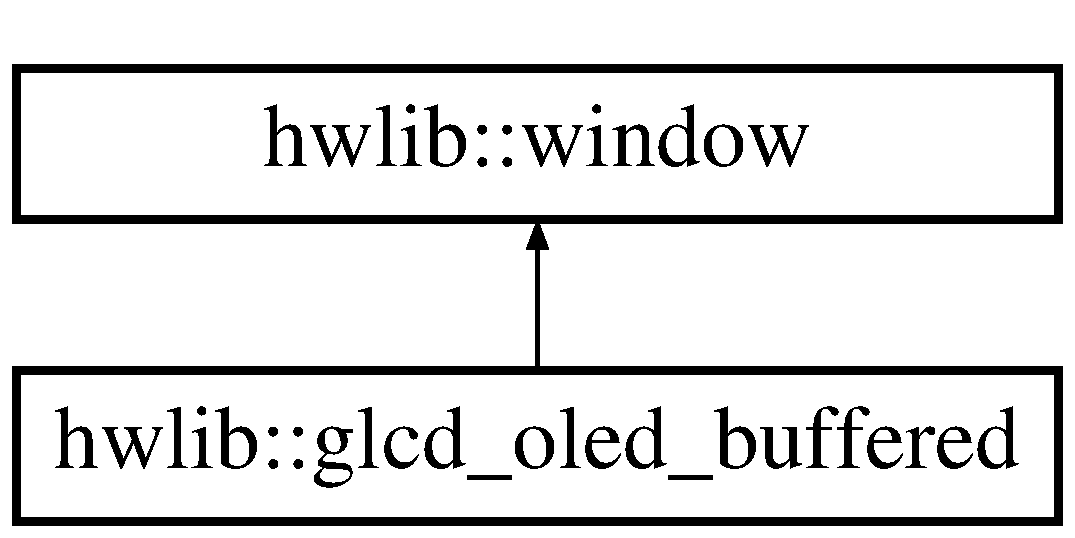
\includegraphics[height=2.000000cm]{classhwlib_1_1glcd__oled__buffered}
\end{center}
\end{figure}
\subsection*{Public Member Functions}
\begin{DoxyCompactItemize}
\item 
{\bfseries glcd\+\_\+oled\+\_\+buffered} (\hyperlink{classhwlib_1_1i2c__bus}{i2c\+\_\+bus} \&bus, \hyperlink{hwlib-defines_8hpp_a54998f25522db04b7b797b0fcc9eb3d5}{fast\+\_\+byte} address=0x3\+C)\hypertarget{classhwlib_1_1glcd__oled__buffered_aefdadf4020316b9392325b5d706e08a9}{}\label{classhwlib_1_1glcd__oled__buffered_aefdadf4020316b9392325b5d706e08a9}

\item 
virtual void \hyperlink{classhwlib_1_1glcd__oled__buffered_a1df3ca6d163e33b2edf1242acf47342a}{clear} ()
\begin{DoxyCompactList}\small\item\em clear the window \end{DoxyCompactList}\item 
void \hyperlink{classhwlib_1_1glcd__oled__buffered_a68ed87e12c7f7ed0abe621b14af9d604}{flush} ()
\begin{DoxyCompactList}\small\item\em write the pixel buffer to the oled \end{DoxyCompactList}\end{DoxyCompactItemize}
\subsection*{Additional Inherited Members}


\subsection{Detailed Description}
Oled B/W graphics L\+CD, buffered. 

This class implements a {\itshape buffered} interface to an 128 x 64 pixel monochrome (on/off) O\+L\+ED display. Buffering means that all writes are buffered in memory until \hyperlink{classhwlib_1_1glcd__oled__buffered_a68ed87e12c7f7ed0abe621b14af9d604}{flush()} is called.

These displays are available in various colcors (green, red, white, etc.). The interface is I2C. The driver chip is an S\+S\+D1306.

When the P\+CB has regulator (3-\/legged component) the power can be 3 -\/ 5V. If it hasn\textquotesingle{}t, you can use only 3.\+3V.

There are variations of this display with more pins, which have more interface options (S\+PI as alternative interface).

This type of display is reasonably priced and available from lots of sources. 

\subsection{Member Function Documentation}
\index{hwlib\+::glcd\+\_\+oled\+\_\+buffered@{hwlib\+::glcd\+\_\+oled\+\_\+buffered}!clear@{clear}}
\index{clear@{clear}!hwlib\+::glcd\+\_\+oled\+\_\+buffered@{hwlib\+::glcd\+\_\+oled\+\_\+buffered}}
\subsubsection[{\texorpdfstring{clear()}{clear()}}]{\setlength{\rightskip}{0pt plus 5cm}virtual void hwlib\+::glcd\+\_\+oled\+\_\+buffered\+::clear (
\begin{DoxyParamCaption}
{}
\end{DoxyParamCaption}
)\hspace{0.3cm}{\ttfamily [inline]}, {\ttfamily [virtual]}}\hypertarget{classhwlib_1_1glcd__oled__buffered_a1df3ca6d163e33b2edf1242acf47342a}{}\label{classhwlib_1_1glcd__oled__buffered_a1df3ca6d163e33b2edf1242acf47342a}


clear the window 

This function clears the windows by writing the background color to all pixels. The default implementation writes to all pixels in sequence. A concrete window can probably provide a faster implementation. 

Reimplemented from \hyperlink{classhwlib_1_1window_a5e781163353ce26cb4dc5b2cbe40ad05}{hwlib\+::window}.

\index{hwlib\+::glcd\+\_\+oled\+\_\+buffered@{hwlib\+::glcd\+\_\+oled\+\_\+buffered}!flush@{flush}}
\index{flush@{flush}!hwlib\+::glcd\+\_\+oled\+\_\+buffered@{hwlib\+::glcd\+\_\+oled\+\_\+buffered}}
\subsubsection[{\texorpdfstring{flush()}{flush()}}]{\setlength{\rightskip}{0pt plus 5cm}void hwlib\+::glcd\+\_\+oled\+\_\+buffered\+::flush (
\begin{DoxyParamCaption}
{}
\end{DoxyParamCaption}
)\hspace{0.3cm}{\ttfamily [inline]}}\hypertarget{classhwlib_1_1glcd__oled__buffered_a68ed87e12c7f7ed0abe621b14af9d604}{}\label{classhwlib_1_1glcd__oled__buffered_a68ed87e12c7f7ed0abe621b14af9d604}


write the pixel buffer to the oled 

All write (and clear) calls change only the in-\/memory pixel buffer. This call writes this pixel buffer to the oled. 

The documentation for this class was generated from the following file\+:\begin{DoxyCompactItemize}
\item 
\hyperlink{hwlib-glcd-oled_8hpp}{hwlib-\/glcd-\/oled.\+hpp}\end{DoxyCompactItemize}

\hypertarget{classhwlib_1_1hc595}{}\section{hwlib\+:\+:hc595 Class Reference}
\label{classhwlib_1_1hc595}\index{hwlib\+::hc595@{hwlib\+::hc595}}


\hyperlink{classhwlib_1_1hc595}{hc595} 8-\/bit output shift register  




{\ttfamily \#include $<$hwlib-\/hc595.\+hpp$>$}

Inheritance diagram for hwlib\+:\+:hc595\+:\begin{figure}[H]
\begin{center}
\leavevmode
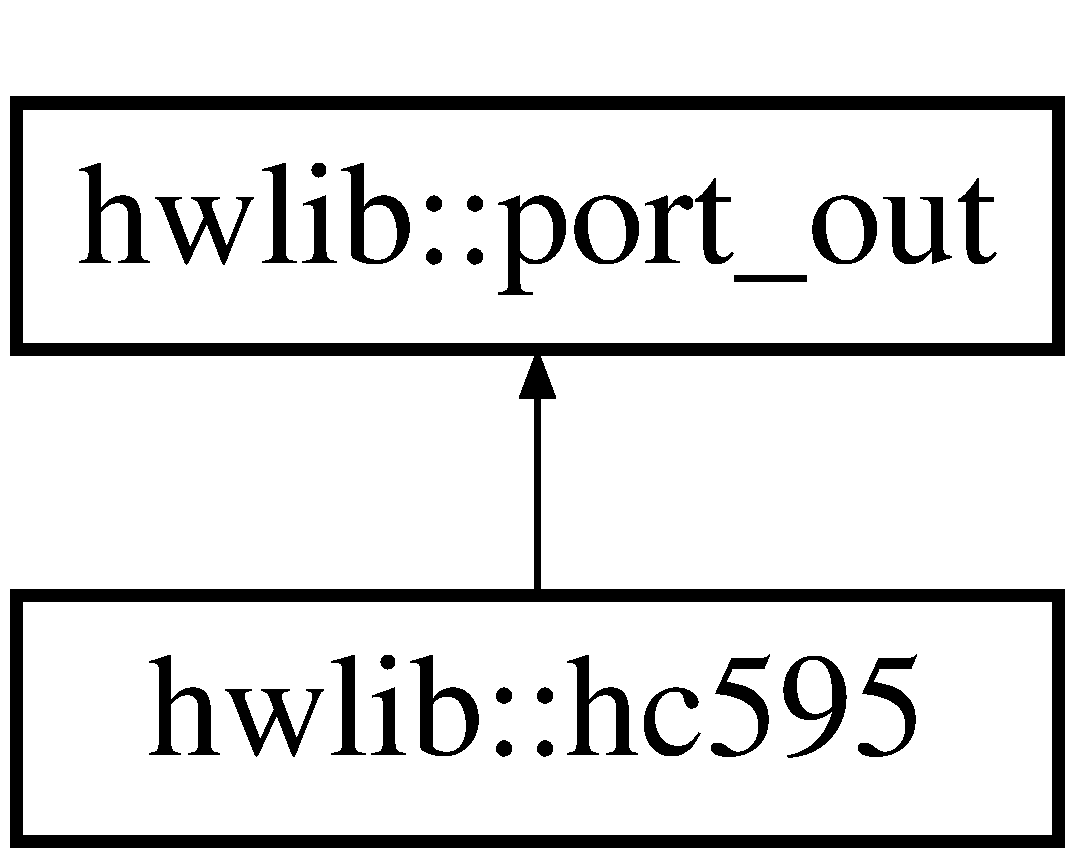
\includegraphics[height=2.000000cm]{classhwlib_1_1hc595}
\end{center}
\end{figure}
\subsection*{Public Types}
\begin{DoxyCompactItemize}
\item 
typedef \+\_\+one\+\_\+pin {\bfseries one\+\_\+pin}\hypertarget{classhwlib_1_1hc595_a9c90bea07c20efa7e90191c25a2ecb35}{}\label{classhwlib_1_1hc595_a9c90bea07c20efa7e90191c25a2ecb35}

\end{DoxyCompactItemize}
\subsection*{Public Member Functions}
\begin{DoxyCompactItemize}
\item 
\hyperlink{classhwlib_1_1hc595_a293236ae5bd14fa376d8b540324f07c0}{hc595} (\hyperlink{classhwlib_1_1spi__bus}{spi\+\_\+bus} \&bus, \hyperlink{classhwlib_1_1pin__out}{pin\+\_\+out} \&sel)
\begin{DoxyCompactList}\small\item\em construct an interface to an \hyperlink{classhwlib_1_1hc595}{hc595} chip \end{DoxyCompactList}\item 
uint\+\_\+fast8\+\_\+t \hyperlink{classhwlib_1_1hc595_a89c7b21cb99d61c91f764a0fdb7ceb9b}{number\+\_\+of\+\_\+pins} () override
\begin{DoxyCompactList}\small\item\em get number of pins \end{DoxyCompactList}\item 
void \hyperlink{classhwlib_1_1hc595_ad2b4d6fa77114f1f13348075389efd1c}{set} (uint\+\_\+fast8\+\_\+t x) override
\begin{DoxyCompactList}\small\item\em write to the port \end{DoxyCompactList}\end{DoxyCompactItemize}
\subsection*{Public Attributes}
{\bf }\par
\begin{DoxyCompactItemize}
\item 
one\+\_\+pin \hyperlink{classhwlib_1_1hc595_a5e124516aa762629f95c7ab63e0b3d18}{p0} \{ $\ast$this, 0 \}
\begin{DoxyCompactList}\small\item\em the output pins of the chip \end{DoxyCompactList}\item 
one\+\_\+pin {\bfseries p1} \{ $\ast$this, 1 \}\hypertarget{classhwlib_1_1hc595_a2f83cce5a65436a22b18a9eae016535c}{}\label{classhwlib_1_1hc595_a2f83cce5a65436a22b18a9eae016535c}

\item 
one\+\_\+pin {\bfseries p2} \{ $\ast$this, 2 \}\hypertarget{classhwlib_1_1hc595_abcdcdb111610864066f7dcb601473c26}{}\label{classhwlib_1_1hc595_abcdcdb111610864066f7dcb601473c26}

\item 
one\+\_\+pin {\bfseries p3} \{ $\ast$this, 3 \}\hypertarget{classhwlib_1_1hc595_a1e2958a2516802e2d6010f53c26802bd}{}\label{classhwlib_1_1hc595_a1e2958a2516802e2d6010f53c26802bd}

\item 
one\+\_\+pin {\bfseries p4} \{ $\ast$this, 4 \}\hypertarget{classhwlib_1_1hc595_ac0b7be902f6bcaeccc77eaac57836131}{}\label{classhwlib_1_1hc595_ac0b7be902f6bcaeccc77eaac57836131}

\item 
one\+\_\+pin {\bfseries p5} \{ $\ast$this, 5 \}\hypertarget{classhwlib_1_1hc595_a071e5983d048d42902099cd432b11cae}{}\label{classhwlib_1_1hc595_a071e5983d048d42902099cd432b11cae}

\item 
one\+\_\+pin {\bfseries p6} \{ $\ast$this, 6 \}\hypertarget{classhwlib_1_1hc595_a0e6cc70a4cb74a6a00f7d65f41744646}{}\label{classhwlib_1_1hc595_a0e6cc70a4cb74a6a00f7d65f41744646}

\item 
one\+\_\+pin {\bfseries p7} \{ $\ast$this, 7 \}\hypertarget{classhwlib_1_1hc595_a28075ecea47020c790ea098e32ab0b5f}{}\label{classhwlib_1_1hc595_a28075ecea47020c790ea098e32ab0b5f}

\end{DoxyCompactItemize}



\subsection{Detailed Description}
\hyperlink{classhwlib_1_1hc595}{hc595} 8-\/bit output shift register 

This class implements an interface to an \hyperlink{classhwlib_1_1hc595}{hc595} 8-\/bit output shift register chip.



The \hyperlink{classhwlib_1_1hc595}{hc595} is an 8-\/bit serial-\/in parallel-\/out shift register, connected to an 8-\/bit data storage register. The 8 outputs of the data register are available on chip pins. The power supply range is 2.\+0 .. 6.\+0 Volt.



The H\+C595 can be used as S\+PI output-\/only peripheral\+:
\begin{DoxyItemize}
\item connect MR (active-\/low reset input) to the power
\item connect OE (active-\/low output enable) to gound
\item use DS as M\+O\+SI
\item use S\+H\+CP as S\+L\+CK
\item use S\+T\+CP as SS
\end{DoxyItemize}

Note that S\+T\+CP is not a real chip-\/select\+: the chip will always respond to the data that is clocked by storing it in the shift register. But only the chip that got the select signal will (on the rising edge of the SS) transfer the data from the shift register to the storage register, hence affecting the outputs. The 74\+H\+C\+T595 is a similar chip, but intended (only) for 5V power, and for use with the old T\+TL signal levels (HC chips are for the C\+M\+OS signal levels that are more common now).

references\+:
\begin{DoxyItemize}
\item \href{https://www.nxp.com/documents/data_sheet/74HC_HCT595.pdf}{\tt 74\+H\+C595/74\+H\+C\+T595 data sheet} (nxp, pdf) 
\end{DoxyItemize}

\subsection{Constructor \& Destructor Documentation}
\index{hwlib\+::hc595@{hwlib\+::hc595}!hc595@{hc595}}
\index{hc595@{hc595}!hwlib\+::hc595@{hwlib\+::hc595}}
\subsubsection[{\texorpdfstring{hc595(spi\+\_\+bus \&bus, pin\+\_\+out \&sel)}{hc595(spi_bus &bus, pin_out &sel)}}]{\setlength{\rightskip}{0pt plus 5cm}hwlib\+::hc595\+::hc595 (
\begin{DoxyParamCaption}
\item[{{\bf spi\+\_\+bus} \&}]{bus, }
\item[{{\bf pin\+\_\+out} \&}]{sel}
\end{DoxyParamCaption}
)\hspace{0.3cm}{\ttfamily [inline]}}\hypertarget{classhwlib_1_1hc595_a293236ae5bd14fa376d8b540324f07c0}{}\label{classhwlib_1_1hc595_a293236ae5bd14fa376d8b540324f07c0}


construct an interface to an \hyperlink{classhwlib_1_1hc595}{hc595} chip 

This constructor creates an interface to an \hyperlink{classhwlib_1_1hc595}{hc595} 8-\/bit output shift register chip from the S\+PI bus it is connected to and and the active-\/low chip select line. 

\subsection{Member Function Documentation}
\index{hwlib\+::hc595@{hwlib\+::hc595}!number\+\_\+of\+\_\+pins@{number\+\_\+of\+\_\+pins}}
\index{number\+\_\+of\+\_\+pins@{number\+\_\+of\+\_\+pins}!hwlib\+::hc595@{hwlib\+::hc595}}
\subsubsection[{\texorpdfstring{number\+\_\+of\+\_\+pins() override}{number_of_pins() override}}]{\setlength{\rightskip}{0pt plus 5cm}uint\+\_\+fast8\+\_\+t hwlib\+::hc595\+::number\+\_\+of\+\_\+pins (
\begin{DoxyParamCaption}
{}
\end{DoxyParamCaption}
)\hspace{0.3cm}{\ttfamily [inline]}, {\ttfamily [override]}, {\ttfamily [virtual]}}\hypertarget{classhwlib_1_1hc595_a89c7b21cb99d61c91f764a0fdb7ceb9b}{}\label{classhwlib_1_1hc595_a89c7b21cb99d61c91f764a0fdb7ceb9b}


get number of pins 

This function returns the number of pins in the port. 

Implements \hyperlink{classhwlib_1_1port__out_a8593e2ff755b938797defb06c1e085df}{hwlib\+::port\+\_\+out}.

\index{hwlib\+::hc595@{hwlib\+::hc595}!set@{set}}
\index{set@{set}!hwlib\+::hc595@{hwlib\+::hc595}}
\subsubsection[{\texorpdfstring{set(uint\+\_\+fast8\+\_\+t x) override}{set(uint_fast8_t x) override}}]{\setlength{\rightskip}{0pt plus 5cm}void hwlib\+::hc595\+::set (
\begin{DoxyParamCaption}
\item[{uint\+\_\+fast8\+\_\+t}]{x}
\end{DoxyParamCaption}
)\hspace{0.3cm}{\ttfamily [inline]}, {\ttfamily [override]}, {\ttfamily [virtual]}}\hypertarget{classhwlib_1_1hc595_ad2b4d6fa77114f1f13348075389efd1c}{}\label{classhwlib_1_1hc595_ad2b4d6fa77114f1f13348075389efd1c}


write to the port 

This function writes to the pins that are part of the port. The lowest bit is written to the first pin of the port, etc. 

Implements \hyperlink{classhwlib_1_1port__out_ad086f5dd66f293118df6ab979feb64fc}{hwlib\+::port\+\_\+out}.



\subsection{Member Data Documentation}
\index{hwlib\+::hc595@{hwlib\+::hc595}!p0@{p0}}
\index{p0@{p0}!hwlib\+::hc595@{hwlib\+::hc595}}
\subsubsection[{\texorpdfstring{p0}{p0}}]{\setlength{\rightskip}{0pt plus 5cm}one\+\_\+pin hwlib\+::hc595\+::p0 \{ $\ast$this, 0 \}}\hypertarget{classhwlib_1_1hc595_a5e124516aa762629f95c7ab63e0b3d18}{}\label{classhwlib_1_1hc595_a5e124516aa762629f95c7ab63e0b3d18}


the output pins of the chip 

The p0 ... p7 attributes represent the 8 output pins of the chip. A write to one of these pins will affect (only) the corresponding output pin of the chip. 

The documentation for this class was generated from the following file\+:\begin{DoxyCompactItemize}
\item 
\hyperlink{hwlib-hc595_8hpp}{hwlib-\/hc595.\+hpp}\end{DoxyCompactItemize}

\hypertarget{classhwlib_1_1hd44780}{}\section{hwlib\+:\+:hd44780 Class Reference}
\label{classhwlib_1_1hd44780}\index{hwlib\+::hd44780@{hwlib\+::hd44780}}


\hyperlink{classhwlib_1_1hd44780}{hd44780} character L\+CD interface  




{\ttfamily \#include $<$hwlib-\/hd44780.\+hpp$>$}

Inheritance diagram for hwlib\+:\+:hd44780\+:\begin{figure}[H]
\begin{center}
\leavevmode
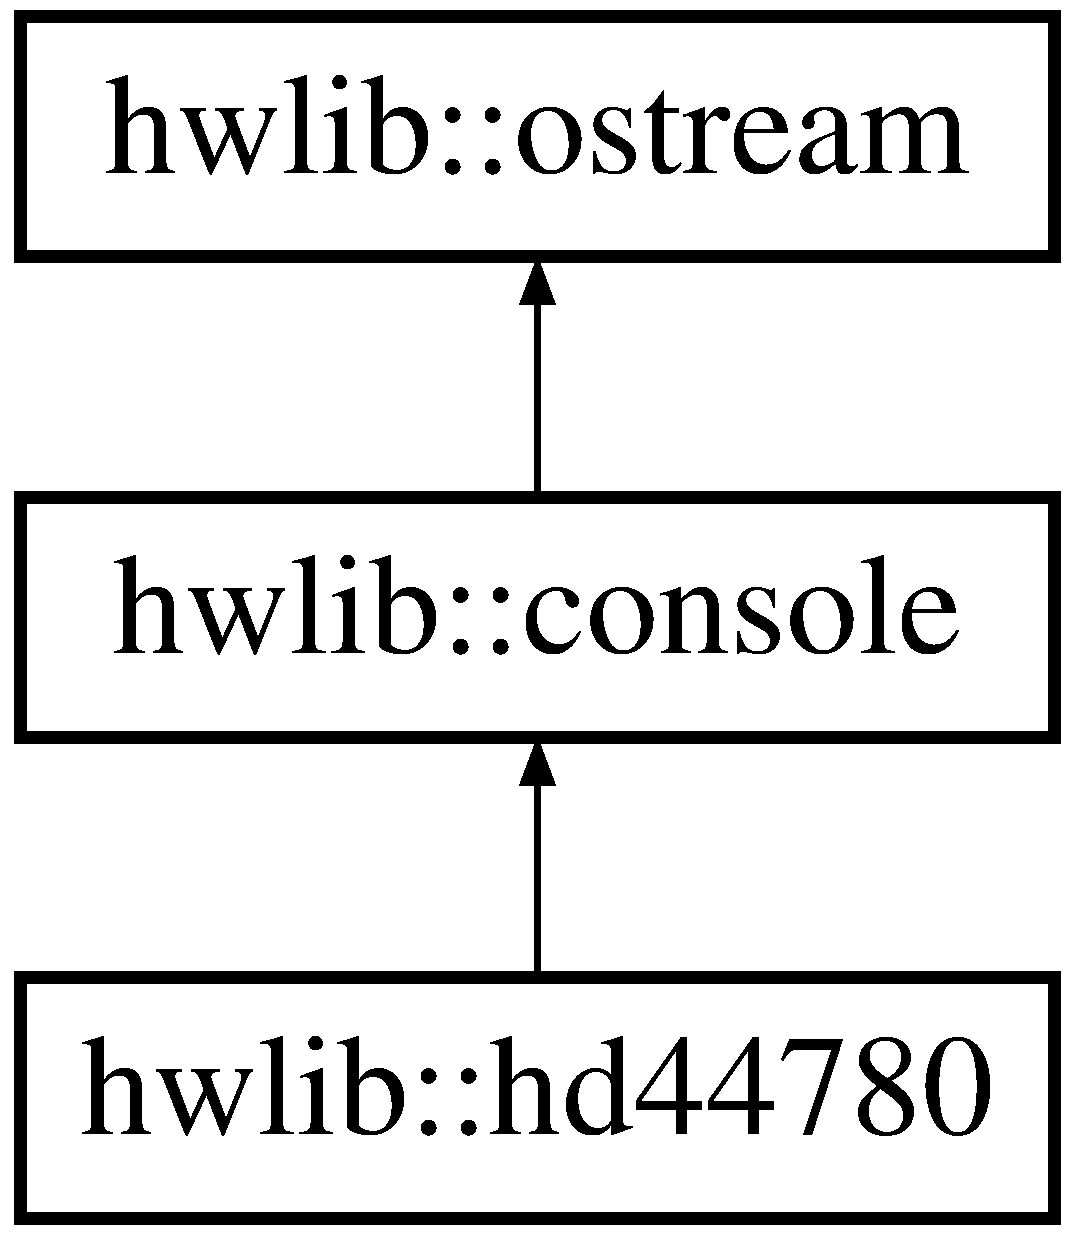
\includegraphics[height=3.000000cm]{classhwlib_1_1hd44780}
\end{center}
\end{figure}
\subsection*{Public Member Functions}
\begin{DoxyCompactItemize}
\item 
\hyperlink{classhwlib_1_1hd44780_a36e0fde84edc8baf6e1362277c11d6c0}{hd44780} (\hyperlink{classhwlib_1_1pin__out}{pin\+\_\+out} \&rs, \hyperlink{classhwlib_1_1pin__out}{pin\+\_\+out} \&e, \hyperlink{classhwlib_1_1port__out}{port\+\_\+out} \&\hyperlink{classhwlib_1_1hd44780_a9a80f74a98efab5fe3a78e8649fd95bb}{data}, int \hyperlink{classhwlib_1_1console_a7c5ec25f5c780aaa56702778701ee270}{lines}, int \hyperlink{classhwlib_1_1console_a5dbe79428aadd15210029a76cb3d255d}{columns})
\begin{DoxyCompactList}\small\item\em construct an interface to an \hyperlink{classhwlib_1_1hd44780}{hd44780} chip \end{DoxyCompactList}\item 
void \hyperlink{classhwlib_1_1hd44780_aa2f8b43bd269d52dd281ec9e90a54f19}{command} (unsigned char cmd)
\begin{DoxyCompactList}\small\item\em write a command byte to the L\+CD \end{DoxyCompactList}\item 
void \hyperlink{classhwlib_1_1hd44780_a9a80f74a98efab5fe3a78e8649fd95bb}{data} (unsigned char chr)
\begin{DoxyCompactList}\small\item\em write a data byte to the L\+CD \end{DoxyCompactList}\item 
void \hyperlink{classhwlib_1_1hd44780_a45d4a84c9da66fa350270df482c6e58f}{clear} () override
\begin{DoxyCompactList}\small\item\em clear the console \end{DoxyCompactList}\end{DoxyCompactItemize}
\subsection*{Additional Inherited Members}


\subsection{Detailed Description}
\hyperlink{classhwlib_1_1hd44780}{hd44780} character L\+CD interface 

This class implements an interface to an \hyperlink{classhwlib_1_1hd44780}{hd44780} character L\+CD.



The \hyperlink{classhwlib_1_1hd44780}{hd44780} is the standard chip for interfacing small dot-\/character L\+CD interfaces. It can display the A\+S\+C\+II table characters, 8 characters (0..7) that can be user-\/defined as 5x7 pixels, and a an upper 128 characters (128...255) that vary with the chip variant, often Japanese characters.

The chip and its digital pins run at 5V. The contrast input can in most cases be connected to 0V (ground), but better is to use a 10k potentiometer between 0V and 5V. Some displays (mostly extended-\/temperature-\/range types) need the lower size of this potentiometer tied to a negative voltage, for instance -\/5V.

The digital interface to the chip has 8 data lines, but the chip can be configured to use only 4. This adds some complexity to the driver software and slows it down a little, but the saving of 4 micro-\/controller more than compensates for this, hence nearly all software (including this driver) for is for the 4-\/bit interface. Note for the 4-\/bit interface the 4 highest data pins (D4..D7) are used. The lower 4 can be left unconnected.

The chip has some locations that can be writen and also read back, but this offers little advantage, so most software (including this driver) only writes to the chip, thus saving another pin. Hence 6 pins (+ ground and 5V) are needed to interface to an \hyperlink{classhwlib_1_1hd44780}{hd44780} display\+: 4 data lines, the R/S line (selects between command and data), and the E line (a strobe for the command).



(Some larger displays use not one but two \hyperlink{classhwlib_1_1hd44780}{hd44780} chips. This interface is not compatible with such L\+C\+Ds.)

Most \hyperlink{classhwlib_1_1hd44780}{hd44780} L\+C\+Ds have a single row of connections, with the following pinout\+:



But as always, check the datasheet (in this case of the L\+CD) to be sure!

The \hyperlink{classhwlib_1_1hd44780}{hd44780} implements the ostream interface, but it doesn\textquotesingle{}t scroll\+: while the cursor is outside the visible characters (beyond the end of the line, or beyond the number of lines) any character writes will be ignored. Some characters are treated special\+:
\begin{DoxyItemize}
\item \textquotesingle{}\textbackslash{}n\textquotesingle{} clears the rest of the line, and then moves to the first position of the next line
\item \textquotesingle{}\textbackslash{}r\textquotesingle{} puts the cursor at the start of the current line
\item \textquotesingle{}\textbackslash{}c\textquotesingle{} moves the cursor to the top-\/left position
\end{DoxyItemize}

The best way to get a flicker-\/free display is to overwite instead of clear-\/and-\/then-\/write\+: use \textquotesingle{}{\ttfamily }\textquotesingle{} to got to the \textquotesingle{}origin\textquotesingle{}, then rewrite the whole display, using \textquotesingle{}~\newline
\textquotesingle{} to go to a next line (because it clears the remainder of the line).

references\+:
\begin{DoxyItemize}
\item \href{https://en.wikipedia.org/wiki/Hitachi_HD44780_LCD_controller}{\tt Hitachi H\+D44780 L\+CD controller} (wikipedia)
\item \href{https://www.sparkfun.com/datasheets/LCD/HD44780.pdf}{\tt H\+D44780U data sheet} (pdf) 
\end{DoxyItemize}

\subsection{Constructor \& Destructor Documentation}
\index{hwlib\+::hd44780@{hwlib\+::hd44780}!hd44780@{hd44780}}
\index{hd44780@{hd44780}!hwlib\+::hd44780@{hwlib\+::hd44780}}
\subsubsection[{\texorpdfstring{hd44780(pin\+\_\+out \&rs, pin\+\_\+out \&e, port\+\_\+out \&data, int lines, int columns)}{hd44780(pin_out &rs, pin_out &e, port_out &data, int lines, int columns)}}]{\setlength{\rightskip}{0pt plus 5cm}hwlib\+::hd44780\+::hd44780 (
\begin{DoxyParamCaption}
\item[{{\bf pin\+\_\+out} \&}]{rs, }
\item[{{\bf pin\+\_\+out} \&}]{e, }
\item[{{\bf port\+\_\+out} \&}]{data, }
\item[{int}]{lines, }
\item[{int}]{columns}
\end{DoxyParamCaption}
)\hspace{0.3cm}{\ttfamily [inline]}}\hypertarget{classhwlib_1_1hd44780_a36e0fde84edc8baf6e1362277c11d6c0}{}\label{classhwlib_1_1hd44780_a36e0fde84edc8baf6e1362277c11d6c0}


construct an interface to an \hyperlink{classhwlib_1_1hd44780}{hd44780} chip 

This constructor creates an interface to an \hyperlink{classhwlib_1_1hd44780}{hd44780} L\+CD controller from the RS and E pins, and the 4-\/bit port to the D4..D8 pins, and the number of lines and characters per line, and initializes the controller. 

\subsection{Member Function Documentation}
\index{hwlib\+::hd44780@{hwlib\+::hd44780}!clear@{clear}}
\index{clear@{clear}!hwlib\+::hd44780@{hwlib\+::hd44780}}
\subsubsection[{\texorpdfstring{clear() override}{clear() override}}]{\setlength{\rightskip}{0pt plus 5cm}void hwlib\+::hd44780\+::clear (
\begin{DoxyParamCaption}
{}
\end{DoxyParamCaption}
)\hspace{0.3cm}{\ttfamily [inline]}, {\ttfamily [override]}, {\ttfamily [virtual]}}\hypertarget{classhwlib_1_1hd44780_a45d4a84c9da66fa350270df482c6e58f}{}\label{classhwlib_1_1hd44780_a45d4a84c9da66fa350270df482c6e58f}


clear the console 

This function clears the console and puts the cursor at (0,0). The default implementation does this by writing spaces to all locations. A concrete implementation might provide a better (faster) way. 

Reimplemented from \hyperlink{classhwlib_1_1console_a6cc5c79177e0fa54e8fb0e50e30c1d30}{hwlib\+::console}.

\index{hwlib\+::hd44780@{hwlib\+::hd44780}!command@{command}}
\index{command@{command}!hwlib\+::hd44780@{hwlib\+::hd44780}}
\subsubsection[{\texorpdfstring{command(unsigned char cmd)}{command(unsigned char cmd)}}]{\setlength{\rightskip}{0pt plus 5cm}void hwlib\+::hd44780\+::command (
\begin{DoxyParamCaption}
\item[{unsigned char}]{cmd}
\end{DoxyParamCaption}
)\hspace{0.3cm}{\ttfamily [inline]}}\hypertarget{classhwlib_1_1hd44780_aa2f8b43bd269d52dd281ec9e90a54f19}{}\label{classhwlib_1_1hd44780_aa2f8b43bd269d52dd281ec9e90a54f19}


write a command byte to the L\+CD 

Use this function only for features that are not provided by the console interface, like the definition of the user-\/defined characters. \index{hwlib\+::hd44780@{hwlib\+::hd44780}!data@{data}}
\index{data@{data}!hwlib\+::hd44780@{hwlib\+::hd44780}}
\subsubsection[{\texorpdfstring{data(unsigned char chr)}{data(unsigned char chr)}}]{\setlength{\rightskip}{0pt plus 5cm}void hwlib\+::hd44780\+::data (
\begin{DoxyParamCaption}
\item[{unsigned char}]{chr}
\end{DoxyParamCaption}
)\hspace{0.3cm}{\ttfamily [inline]}}\hypertarget{classhwlib_1_1hd44780_a9a80f74a98efab5fe3a78e8649fd95bb}{}\label{classhwlib_1_1hd44780_a9a80f74a98efab5fe3a78e8649fd95bb}


write a data byte to the L\+CD 

Use this function only for features that are not provided by the console interface, like the definition of the user-\/defined characters. 

The documentation for this class was generated from the following file\+:\begin{DoxyCompactItemize}
\item 
\hyperlink{hwlib-hd44780_8hpp}{hwlib-\/hd44780.\+hpp}\end{DoxyCompactItemize}

\hypertarget{classhwlib_1_1i2c__bus}{}\section{hwlib\+:\+:i2c\+\_\+bus Class Reference}
\label{classhwlib_1_1i2c__bus}\index{hwlib\+::i2c\+\_\+bus@{hwlib\+::i2c\+\_\+bus}}


i2c bus master interface  




{\ttfamily \#include $<$hwlib-\/i2c.\+hpp$>$}

Inheritance diagram for hwlib\+:\+:i2c\+\_\+bus\+:\begin{figure}[H]
\begin{center}
\leavevmode
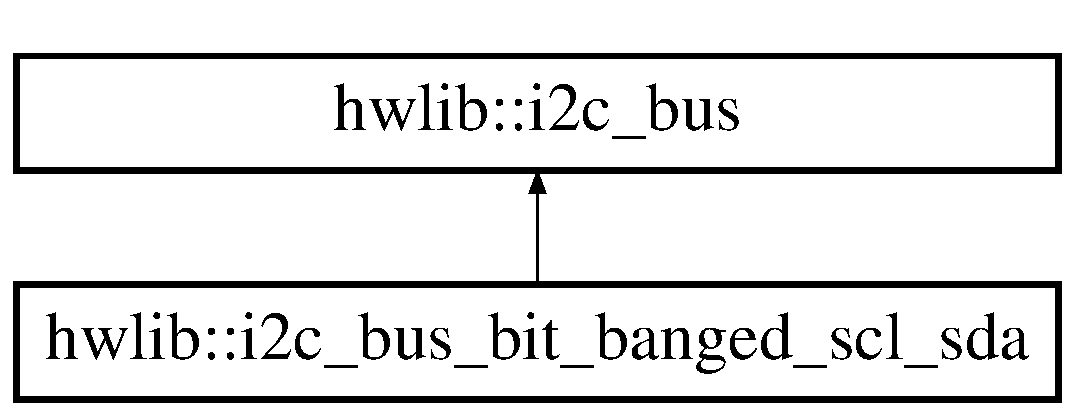
\includegraphics[height=2.000000cm]{classhwlib_1_1i2c__bus}
\end{center}
\end{figure}
\subsection*{Public Member Functions}
\begin{DoxyCompactItemize}
\item 
virtual void \hyperlink{classhwlib_1_1i2c__bus_ab61d2f9d41ce7c019599fcbb87a420c0}{write} (\hyperlink{hwlib-defines_8hpp_a54998f25522db04b7b797b0fcc9eb3d5}{fast\+\_\+byte} a, const \hyperlink{hwlib-defines_8hpp_ab8ef12fab634c171394422d0ee8baf94}{byte} data\mbox{[}$\,$\mbox{]}, \hyperlink{hwlib-defines_8hpp_a54998f25522db04b7b797b0fcc9eb3d5}{fast\+\_\+byte} n)=0
\begin{DoxyCompactList}\small\item\em i2c write transaction \end{DoxyCompactList}\item 
virtual void \hyperlink{classhwlib_1_1i2c__bus_a389ef0c95c69657e1b36352f16d824d8}{read} (\hyperlink{hwlib-defines_8hpp_a54998f25522db04b7b797b0fcc9eb3d5}{fast\+\_\+byte} a, \hyperlink{hwlib-defines_8hpp_ab8ef12fab634c171394422d0ee8baf94}{byte} data\mbox{[}$\,$\mbox{]}, \hyperlink{hwlib-defines_8hpp_a54998f25522db04b7b797b0fcc9eb3d5}{fast\+\_\+byte} n)=0
\begin{DoxyCompactList}\small\item\em i2c read transaction \end{DoxyCompactList}\end{DoxyCompactItemize}


\subsection{Detailed Description}
i2c bus master interface 

This class abstracts the interface of a master to an I2C bus.

In its simplest form, an I2C bus has one master and a number of slaves that are connected by two wires\+: S\+CL (clock) and S\+DA (data). Both lines are pulled up by pull-\/up resistor, and can (only) be pulled down by a connected chip (open-\/collector).



An I2C transaction is either a read transaction or a transaction. In both cases, the transaction starts with the master transmitting a control byte, which contains the address of the slave chip, and one bit that indicates whether it is a read or a write transaction. The bits of a byte are transferred M\+SB (most significant bit) first.





Next the slave chip receives (write transaction) or transmits (read transaction) as many bytes as the master asks for.



At the bit level, master generates clock pulses by pulling the S\+CL line low. While the S\+CL is low, the master or slave can put a bit on the S\+DA line by pulling it down (for a 0) or letting it float (for a 1). The S\+CL line is always driven by the master (unless the slave uses clock-\/stretching), the S\+DA line is driven by the device on the bus that sends the bit.



Two special conditions are used. To signal the start (S) of a transaction, the sda is pulled low while the clk is high. The reverse is used to indicate a stop (P, the end of a transaction)\+: the dta is released (goes high) while the clock is high.



Most slave chips that have only one data byte that can be read or written use a single-\/byte read or write transmission to read or write that data byte. Slave chips that have more than one address that can be written often use a write transaction where the first byte(s) written determine the address (within the slave chip), and the subsequent byte(s) are written to that address (and to the next addresses). An I2C read transaction addresses the slave chip, but has no provision to specify an address within the slave chip. A common trick is that a read addresses the last address specified by a (previous) write transaction. Hence to read from address X first a write is done to address X, but the transaaction stops after the X, hence nothing is written, but this sets the address pointer inside the slave chip. Now a read transaction reads from this address.

As always, consult the datasheet of the chip for the details.

The I2C bus was invented by Philips, who had a patent on it. Hence other manufacturers that implemented the I2C bus on their chips had either to pay royalties to Philips, or tried to avoid this by implementing a protocol that was compatible with I2C, without mentioning I2C. The I2C patent has expired, but you can still find many chips that are described as \textquotesingle{}implementing a two-\/wire protocol\textquotesingle{} or something similar. In most cases this means that the chip implements I2C.

references\+:
\begin{DoxyItemize}
\item \href{http://www.nxp.com/documents/user_manual/UM10204.pdf}{\tt I2C bus specification and user manual} (pdf)
\item \href{http://i2c.info/i2c-bus-specification}{\tt I2C Bus Specification} (info page)
\item \href{https://en.wikipedia.org/wiki/I2C}{\tt I2C Bus} (wikipedia) 
\end{DoxyItemize}

\subsection{Member Function Documentation}
\index{hwlib\+::i2c\+\_\+bus@{hwlib\+::i2c\+\_\+bus}!read@{read}}
\index{read@{read}!hwlib\+::i2c\+\_\+bus@{hwlib\+::i2c\+\_\+bus}}
\subsubsection[{\texorpdfstring{read(fast\+\_\+byte a, byte data[], fast\+\_\+byte n)=0}{read(fast_byte a, byte data[], fast_byte n)=0}}]{\setlength{\rightskip}{0pt plus 5cm}virtual void hwlib\+::i2c\+\_\+bus\+::read (
\begin{DoxyParamCaption}
\item[{{\bf fast\+\_\+byte}}]{a, }
\item[{{\bf byte}}]{data\mbox{[}$\,$\mbox{]}, }
\item[{{\bf fast\+\_\+byte}}]{n}
\end{DoxyParamCaption}
)\hspace{0.3cm}{\ttfamily [pure virtual]}}\hypertarget{classhwlib_1_1i2c__bus_a389ef0c95c69657e1b36352f16d824d8}{}\label{classhwlib_1_1i2c__bus_a389ef0c95c69657e1b36352f16d824d8}


i2c read transaction 

This function reads n bytes from the slave at address a to data\mbox{[}\mbox{]}.

Note that n is a byte, hence the maximum number of bytes is 255. 

Implemented in \hyperlink{classhwlib_1_1i2c__bus__bit__banged__scl__sda_a3936c0c4052692b999cf46c9cb12868b}{hwlib\+::i2c\+\_\+bus\+\_\+bit\+\_\+banged\+\_\+scl\+\_\+sda}.

\index{hwlib\+::i2c\+\_\+bus@{hwlib\+::i2c\+\_\+bus}!write@{write}}
\index{write@{write}!hwlib\+::i2c\+\_\+bus@{hwlib\+::i2c\+\_\+bus}}
\subsubsection[{\texorpdfstring{write(fast\+\_\+byte a, const byte data[], fast\+\_\+byte n)=0}{write(fast_byte a, const byte data[], fast_byte n)=0}}]{\setlength{\rightskip}{0pt plus 5cm}virtual void hwlib\+::i2c\+\_\+bus\+::write (
\begin{DoxyParamCaption}
\item[{{\bf fast\+\_\+byte}}]{a, }
\item[{const {\bf byte}}]{data\mbox{[}$\,$\mbox{]}, }
\item[{{\bf fast\+\_\+byte}}]{n}
\end{DoxyParamCaption}
)\hspace{0.3cm}{\ttfamily [pure virtual]}}\hypertarget{classhwlib_1_1i2c__bus_ab61d2f9d41ce7c019599fcbb87a420c0}{}\label{classhwlib_1_1i2c__bus_ab61d2f9d41ce7c019599fcbb87a420c0}


i2c write transaction 

This function write n bytes from data\mbox{[}\mbox{]} to the slave at address a.

Note that n is a byte, hence the maximum number of bytes is 255. 

Implemented in \hyperlink{classhwlib_1_1i2c__bus__bit__banged__scl__sda_a7f030dbd80fee19a6e6a9846e998d411}{hwlib\+::i2c\+\_\+bus\+\_\+bit\+\_\+banged\+\_\+scl\+\_\+sda}.



The documentation for this class was generated from the following file\+:\begin{DoxyCompactItemize}
\item 
\hyperlink{hwlib-i2c_8hpp}{hwlib-\/i2c.\+hpp}\end{DoxyCompactItemize}

\hypertarget{classhwlib_1_1i2c__bus__bit__banged__scl__sda}{}\section{hwlib\+:\+:i2c\+\_\+bus\+\_\+bit\+\_\+banged\+\_\+scl\+\_\+sda Class Reference}
\label{classhwlib_1_1i2c__bus__bit__banged__scl__sda}\index{hwlib\+::i2c\+\_\+bus\+\_\+bit\+\_\+banged\+\_\+scl\+\_\+sda@{hwlib\+::i2c\+\_\+bus\+\_\+bit\+\_\+banged\+\_\+scl\+\_\+sda}}


bit-\/banged i2c bus implementation  




{\ttfamily \#include $<$hwlib-\/i2c.\+hpp$>$}

Inheritance diagram for hwlib\+:\+:i2c\+\_\+bus\+\_\+bit\+\_\+banged\+\_\+scl\+\_\+sda\+:\begin{figure}[H]
\begin{center}
\leavevmode
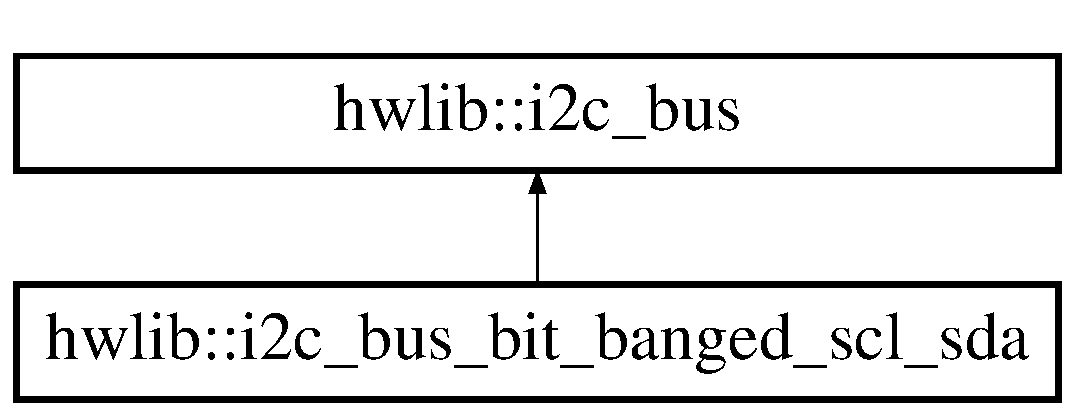
\includegraphics[height=2.000000cm]{classhwlib_1_1i2c__bus__bit__banged__scl__sda}
\end{center}
\end{figure}
\subsection*{Public Member Functions}
\begin{DoxyCompactItemize}
\item 
\hyperlink{classhwlib_1_1i2c__bus__bit__banged__scl__sda_aff6b11113640da8c8f04b60081bef5ae}{i2c\+\_\+bus\+\_\+bit\+\_\+banged\+\_\+scl\+\_\+sda} (\hyperlink{classhwlib_1_1pin__oc}{pin\+\_\+oc} \&scl, \hyperlink{classhwlib_1_1pin__oc}{pin\+\_\+oc} \&sda)
\begin{DoxyCompactList}\small\item\em construct a bit-\/banged I2C bus from the scl and sda pins \end{DoxyCompactList}\item 
void \hyperlink{classhwlib_1_1i2c__bus__bit__banged__scl__sda_a7f030dbd80fee19a6e6a9846e998d411}{write} (\hyperlink{hwlib-defines_8hpp_a54998f25522db04b7b797b0fcc9eb3d5}{fast\+\_\+byte} a, const \hyperlink{hwlib-defines_8hpp_ab8ef12fab634c171394422d0ee8baf94}{byte} data\mbox{[}$\,$\mbox{]}, \hyperlink{hwlib-defines_8hpp_a54998f25522db04b7b797b0fcc9eb3d5}{fast\+\_\+byte} n) override
\begin{DoxyCompactList}\small\item\em write to a connect I2C slave device \end{DoxyCompactList}\item 
void \hyperlink{classhwlib_1_1i2c__bus__bit__banged__scl__sda_a3936c0c4052692b999cf46c9cb12868b}{read} (\hyperlink{hwlib-defines_8hpp_a54998f25522db04b7b797b0fcc9eb3d5}{fast\+\_\+byte} a, \hyperlink{hwlib-defines_8hpp_ab8ef12fab634c171394422d0ee8baf94}{byte} data\mbox{[}$\,$\mbox{]}, \hyperlink{hwlib-defines_8hpp_a54998f25522db04b7b797b0fcc9eb3d5}{fast\+\_\+byte} n) override
\begin{DoxyCompactList}\small\item\em read from a connected I2C slave device \end{DoxyCompactList}\end{DoxyCompactItemize}


\subsection{Detailed Description}
bit-\/banged i2c bus implementation 

This class implements a bit-\/banged master interface to an I2C bus. Limitations\+:
\begin{DoxyItemize}
\item only the 7-\/bit address format is supported
\item clock stretching by the slave is not supporte
\item only a single master is supported
\item the speed is fixed at $\sim$ 100 k\+Hz or somewhat lower 
\end{DoxyItemize}

\subsection{Constructor \& Destructor Documentation}
\index{hwlib\+::i2c\+\_\+bus\+\_\+bit\+\_\+banged\+\_\+scl\+\_\+sda@{hwlib\+::i2c\+\_\+bus\+\_\+bit\+\_\+banged\+\_\+scl\+\_\+sda}!i2c\+\_\+bus\+\_\+bit\+\_\+banged\+\_\+scl\+\_\+sda@{i2c\+\_\+bus\+\_\+bit\+\_\+banged\+\_\+scl\+\_\+sda}}
\index{i2c\+\_\+bus\+\_\+bit\+\_\+banged\+\_\+scl\+\_\+sda@{i2c\+\_\+bus\+\_\+bit\+\_\+banged\+\_\+scl\+\_\+sda}!hwlib\+::i2c\+\_\+bus\+\_\+bit\+\_\+banged\+\_\+scl\+\_\+sda@{hwlib\+::i2c\+\_\+bus\+\_\+bit\+\_\+banged\+\_\+scl\+\_\+sda}}
\subsubsection[{\texorpdfstring{i2c\+\_\+bus\+\_\+bit\+\_\+banged\+\_\+scl\+\_\+sda(pin\+\_\+oc \&scl, pin\+\_\+oc \&sda)}{i2c_bus_bit_banged_scl_sda(pin_oc &scl, pin_oc &sda)}}]{\setlength{\rightskip}{0pt plus 5cm}hwlib\+::i2c\+\_\+bus\+\_\+bit\+\_\+banged\+\_\+scl\+\_\+sda\+::i2c\+\_\+bus\+\_\+bit\+\_\+banged\+\_\+scl\+\_\+sda (
\begin{DoxyParamCaption}
\item[{{\bf pin\+\_\+oc} \&}]{scl, }
\item[{{\bf pin\+\_\+oc} \&}]{sda}
\end{DoxyParamCaption}
)\hspace{0.3cm}{\ttfamily [inline]}}\hypertarget{classhwlib_1_1i2c__bus__bit__banged__scl__sda_aff6b11113640da8c8f04b60081bef5ae}{}\label{classhwlib_1_1i2c__bus__bit__banged__scl__sda_aff6b11113640da8c8f04b60081bef5ae}


construct a bit-\/banged I2C bus from the scl and sda pins 

This constructor creates a bit-\/banged I2C bus master from the scl and sda pins. 

\subsection{Member Function Documentation}
\index{hwlib\+::i2c\+\_\+bus\+\_\+bit\+\_\+banged\+\_\+scl\+\_\+sda@{hwlib\+::i2c\+\_\+bus\+\_\+bit\+\_\+banged\+\_\+scl\+\_\+sda}!read@{read}}
\index{read@{read}!hwlib\+::i2c\+\_\+bus\+\_\+bit\+\_\+banged\+\_\+scl\+\_\+sda@{hwlib\+::i2c\+\_\+bus\+\_\+bit\+\_\+banged\+\_\+scl\+\_\+sda}}
\subsubsection[{\texorpdfstring{read(fast\+\_\+byte a, byte data[], fast\+\_\+byte n) override}{read(fast_byte a, byte data[], fast_byte n) override}}]{\setlength{\rightskip}{0pt plus 5cm}void hwlib\+::i2c\+\_\+bus\+\_\+bit\+\_\+banged\+\_\+scl\+\_\+sda\+::read (
\begin{DoxyParamCaption}
\item[{{\bf fast\+\_\+byte}}]{a, }
\item[{{\bf byte}}]{data\mbox{[}$\,$\mbox{]}, }
\item[{{\bf fast\+\_\+byte}}]{n}
\end{DoxyParamCaption}
)\hspace{0.3cm}{\ttfamily [inline]}, {\ttfamily [override]}, {\ttfamily [virtual]}}\hypertarget{classhwlib_1_1i2c__bus__bit__banged__scl__sda_a3936c0c4052692b999cf46c9cb12868b}{}\label{classhwlib_1_1i2c__bus__bit__banged__scl__sda_a3936c0c4052692b999cf46c9cb12868b}


read from a connected I2C slave device 

This function reads n bytes of data from the device with address a that is connected to the I2C bus. 

Implements \hyperlink{classhwlib_1_1i2c__bus_a389ef0c95c69657e1b36352f16d824d8}{hwlib\+::i2c\+\_\+bus}.

\index{hwlib\+::i2c\+\_\+bus\+\_\+bit\+\_\+banged\+\_\+scl\+\_\+sda@{hwlib\+::i2c\+\_\+bus\+\_\+bit\+\_\+banged\+\_\+scl\+\_\+sda}!write@{write}}
\index{write@{write}!hwlib\+::i2c\+\_\+bus\+\_\+bit\+\_\+banged\+\_\+scl\+\_\+sda@{hwlib\+::i2c\+\_\+bus\+\_\+bit\+\_\+banged\+\_\+scl\+\_\+sda}}
\subsubsection[{\texorpdfstring{write(fast\+\_\+byte a, const byte data[], fast\+\_\+byte n) override}{write(fast_byte a, const byte data[], fast_byte n) override}}]{\setlength{\rightskip}{0pt plus 5cm}void hwlib\+::i2c\+\_\+bus\+\_\+bit\+\_\+banged\+\_\+scl\+\_\+sda\+::write (
\begin{DoxyParamCaption}
\item[{{\bf fast\+\_\+byte}}]{a, }
\item[{const {\bf byte}}]{data\mbox{[}$\,$\mbox{]}, }
\item[{{\bf fast\+\_\+byte}}]{n}
\end{DoxyParamCaption}
)\hspace{0.3cm}{\ttfamily [inline]}, {\ttfamily [override]}, {\ttfamily [virtual]}}\hypertarget{classhwlib_1_1i2c__bus__bit__banged__scl__sda_a7f030dbd80fee19a6e6a9846e998d411}{}\label{classhwlib_1_1i2c__bus__bit__banged__scl__sda_a7f030dbd80fee19a6e6a9846e998d411}


write to a connect I2C slave device 

This function writes n bytes of data to the device with address a that is connected to the I2C bus. 

Implements \hyperlink{classhwlib_1_1i2c__bus_ab61d2f9d41ce7c019599fcbb87a420c0}{hwlib\+::i2c\+\_\+bus}.



The documentation for this class was generated from the following file\+:\begin{DoxyCompactItemize}
\item 
\hyperlink{hwlib-i2c_8hpp}{hwlib-\/i2c.\+hpp}\end{DoxyCompactItemize}

\hypertarget{classhwlib_1_1image}{}\section{hwlib\+:\+:image Class Reference}
\label{classhwlib_1_1image}\index{hwlib\+::image@{hwlib\+::image}}


an image  




{\ttfamily \#include $<$hwlib-\/graphics.\+hpp$>$}

Inheritance diagram for hwlib\+:\+:image\+:\begin{figure}[H]
\begin{center}
\leavevmode
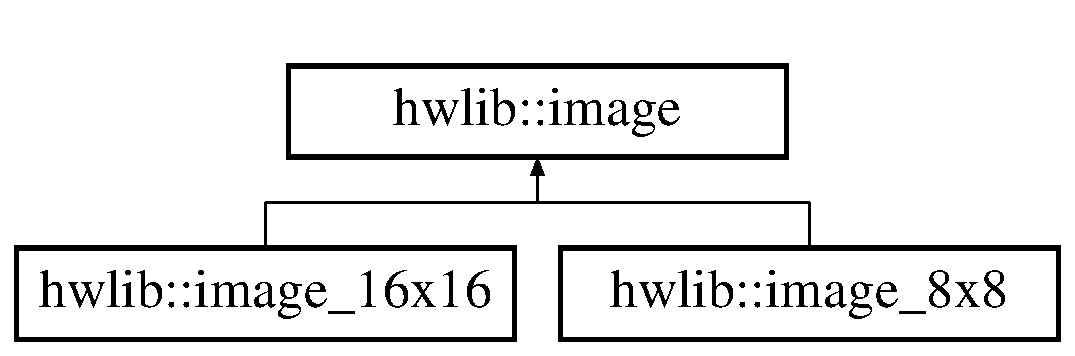
\includegraphics[height=2.000000cm]{classhwlib_1_1image}
\end{center}
\end{figure}
\subsection*{Public Member Functions}
\begin{DoxyCompactItemize}
\item 
constexpr \hyperlink{classhwlib_1_1image_a0546f83e7d9ffa8de211d64925a24d3f}{image} (\hyperlink{classhwlib_1_1location}{location} \hyperlink{classhwlib_1_1image_ab675f56d00632a4099ed9ec1d4539165}{size})\hypertarget{classhwlib_1_1image_a0546f83e7d9ffa8de211d64925a24d3f}{}\label{classhwlib_1_1image_a0546f83e7d9ffa8de211d64925a24d3f}

\begin{DoxyCompactList}\small\item\em construct an image by specifying its size. \end{DoxyCompactList}\item 
\hyperlink{classhwlib_1_1color}{color} \hyperlink{classhwlib_1_1image_acfdcdfcfe6b0902b5428b4c5aaf37671}{operator\mbox{[}$\,$\mbox{]}} (\hyperlink{classhwlib_1_1location}{location} pos) const \hypertarget{classhwlib_1_1image_acfdcdfcfe6b0902b5428b4c5aaf37671}{}\label{classhwlib_1_1image_acfdcdfcfe6b0902b5428b4c5aaf37671}

\begin{DoxyCompactList}\small\item\em return the coclor at the specified location \end{DoxyCompactList}\end{DoxyCompactItemize}
\subsection*{Public Attributes}
\begin{DoxyCompactItemize}
\item 
\hyperlink{classhwlib_1_1location}{location} \hyperlink{classhwlib_1_1image_ab675f56d00632a4099ed9ec1d4539165}{size}
\begin{DoxyCompactList}\small\item\em the size of the image \end{DoxyCompactList}\end{DoxyCompactItemize}


\subsection{Detailed Description}
an image 

An image is a rectangular set of pixel values (colors). 

\subsection{Member Data Documentation}
\index{hwlib\+::image@{hwlib\+::image}!size@{size}}
\index{size@{size}!hwlib\+::image@{hwlib\+::image}}
\subsubsection[{\texorpdfstring{size}{size}}]{\setlength{\rightskip}{0pt plus 5cm}{\bf location} hwlib\+::image\+::size}\hypertarget{classhwlib_1_1image_ab675f56d00632a4099ed9ec1d4539165}{}\label{classhwlib_1_1image_ab675f56d00632a4099ed9ec1d4539165}


the size of the image 

This is the size of the image\+: the number of pixels in the x and y direction. 

The documentation for this class was generated from the following file\+:\begin{DoxyCompactItemize}
\item 
\hyperlink{hwlib-graphics_8hpp}{hwlib-\/graphics.\+hpp}\end{DoxyCompactItemize}

\hypertarget{classhwlib_1_1image__16x16}{}\section{hwlib\+:\+:image\+\_\+16x16 Class Reference}
\label{classhwlib_1_1image__16x16}\index{hwlib\+::image\+\_\+16x16@{hwlib\+::image\+\_\+16x16}}
Inheritance diagram for hwlib\+:\+:image\+\_\+16x16\+:\begin{figure}[H]
\begin{center}
\leavevmode
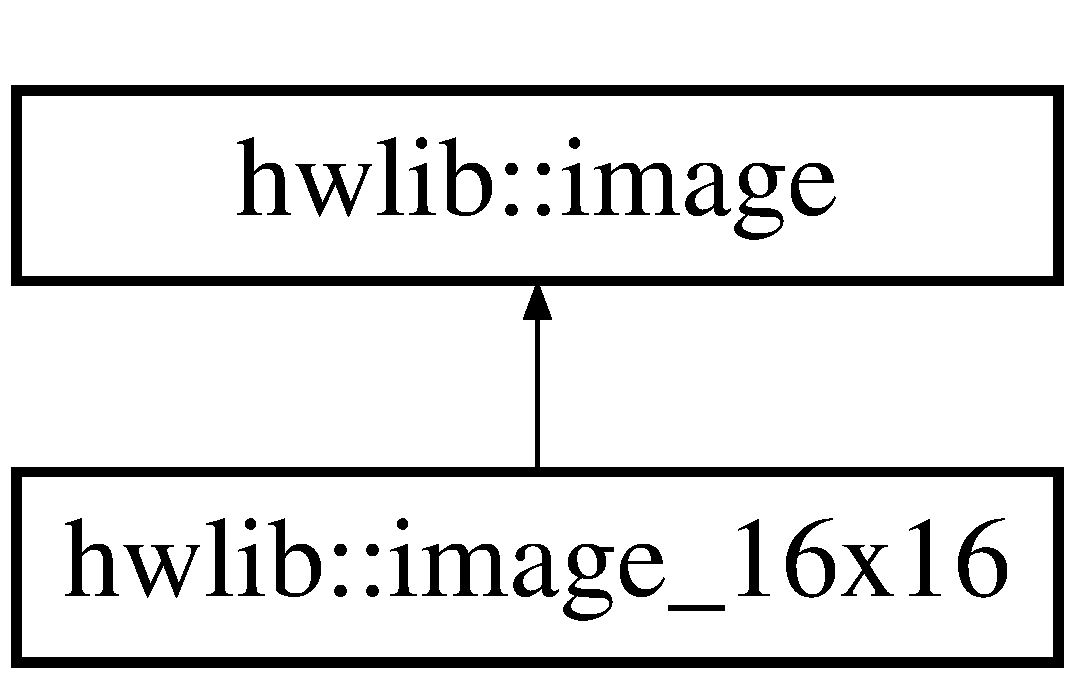
\includegraphics[height=2.000000cm]{classhwlib_1_1image__16x16}
\end{center}
\end{figure}
\subsection*{Public Member Functions}
\begin{DoxyCompactItemize}
\item 
constexpr {\bfseries image\+\_\+16x16} (uint8\+\_\+t $\ast$data)\hypertarget{classhwlib_1_1image__16x16_a55d9a91ab23947cfe7068042400b365a}{}\label{classhwlib_1_1image__16x16_a55d9a91ab23947cfe7068042400b365a}

\end{DoxyCompactItemize}
\subsection*{Additional Inherited Members}


The documentation for this class was generated from the following file\+:\begin{DoxyCompactItemize}
\item 
\hyperlink{hwlib-font-default-16x16_8hpp}{hwlib-\/font-\/default-\/16x16.\+hpp}\end{DoxyCompactItemize}

\hypertarget{classhwlib_1_1image__8x8}{}\section{hwlib\+:\+:image\+\_\+8x8 Class Reference}
\label{classhwlib_1_1image__8x8}\index{hwlib\+::image\+\_\+8x8@{hwlib\+::image\+\_\+8x8}}


an 8x8 pixel image that contains its pixels  




{\ttfamily \#include $<$hwlib-\/graphics.\+hpp$>$}

Inheritance diagram for hwlib\+:\+:image\+\_\+8x8\+:\begin{figure}[H]
\begin{center}
\leavevmode
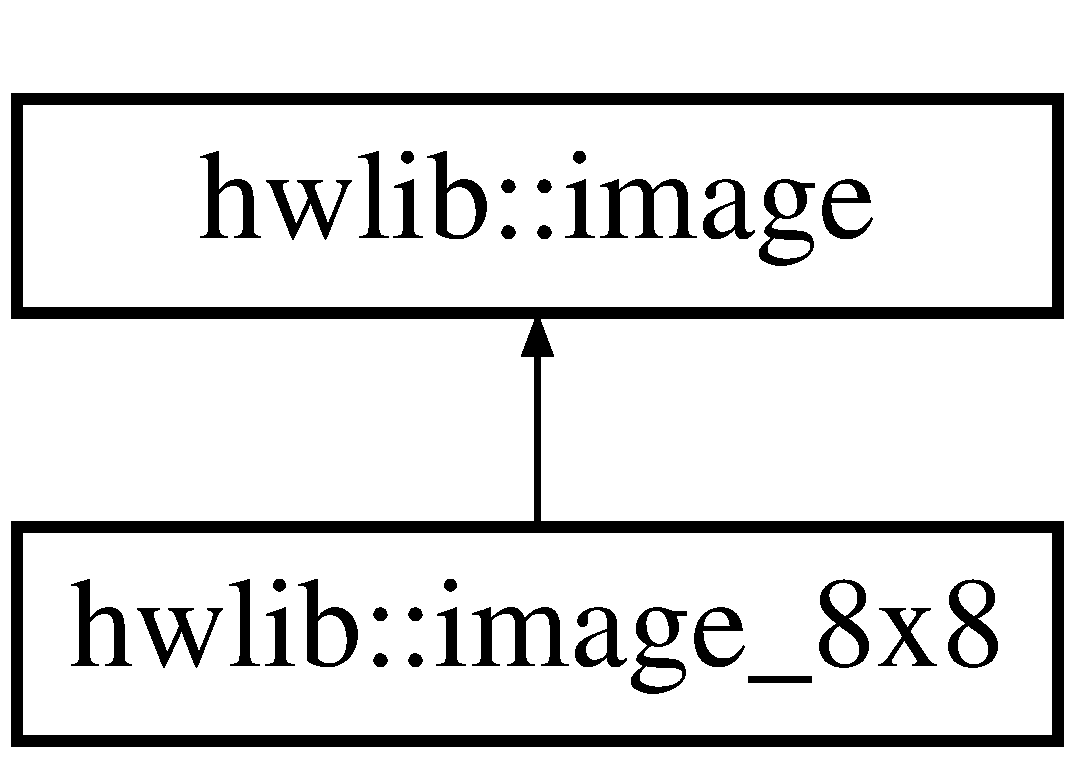
\includegraphics[height=2.000000cm]{classhwlib_1_1image__8x8}
\end{center}
\end{figure}
\subsection*{Public Member Functions}
\begin{DoxyCompactItemize}
\item 
constexpr \hyperlink{classhwlib_1_1image__8x8_a9384d60dbb742e96c3c03792545fbd56}{image\+\_\+8x8} (unsigned char d0, unsigned char d1, unsigned char d2, unsigned char d3, unsigned char d4, unsigned char d5, unsigned char d6, unsigned char d7)
\begin{DoxyCompactList}\small\item\em create the \hyperlink{classhwlib_1_1image__8x8}{image\+\_\+8x8} by supplying the pixels \end{DoxyCompactList}\end{DoxyCompactItemize}
\subsection*{Additional Inherited Members}


\subsection{Detailed Description}
an 8x8 pixel image that contains its pixels 

\subsection{Constructor \& Destructor Documentation}
\index{hwlib\+::image\+\_\+8x8@{hwlib\+::image\+\_\+8x8}!image\+\_\+8x8@{image\+\_\+8x8}}
\index{image\+\_\+8x8@{image\+\_\+8x8}!hwlib\+::image\+\_\+8x8@{hwlib\+::image\+\_\+8x8}}
\subsubsection[{\texorpdfstring{image\+\_\+8x8(unsigned char d0, unsigned char d1, unsigned char d2, unsigned char d3, unsigned char d4, unsigned char d5, unsigned char d6, unsigned char d7)}{image_8x8(unsigned char d0, unsigned char d1, unsigned char d2, unsigned char d3, unsigned char d4, unsigned char d5, unsigned char d6, unsigned char d7)}}]{\setlength{\rightskip}{0pt plus 5cm}constexpr hwlib\+::image\+\_\+8x8\+::image\+\_\+8x8 (
\begin{DoxyParamCaption}
\item[{unsigned char}]{d0, }
\item[{unsigned char}]{d1, }
\item[{unsigned char}]{d2, }
\item[{unsigned char}]{d3, }
\item[{unsigned char}]{d4, }
\item[{unsigned char}]{d5, }
\item[{unsigned char}]{d6, }
\item[{unsigned char}]{d7}
\end{DoxyParamCaption}
)\hspace{0.3cm}{\ttfamily [inline]}}\hypertarget{classhwlib_1_1image__8x8_a9384d60dbb742e96c3c03792545fbd56}{}\label{classhwlib_1_1image__8x8_a9384d60dbb742e96c3c03792545fbd56}


create the \hyperlink{classhwlib_1_1image__8x8}{image\+\_\+8x8} by supplying the pixels 

The d0 argument contains the top row, bit 0 is the leftmost pixel. 

The documentation for this class was generated from the following file\+:\begin{DoxyCompactItemize}
\item 
\hyperlink{hwlib-graphics_8hpp}{hwlib-\/graphics.\+hpp}\end{DoxyCompactItemize}

\hypertarget{classhwlib_1_1istream}{}\section{hwlib\+:\+:istream Class Reference}
\label{classhwlib_1_1istream}\index{hwlib\+::istream@{hwlib\+::istream}}


character input stream  




{\ttfamily \#include $<$hwlib-\/ostream -\/ Copy.\+hpp$>$}

Inheritance diagram for hwlib\+:\+:istream\+:\begin{figure}[H]
\begin{center}
\leavevmode
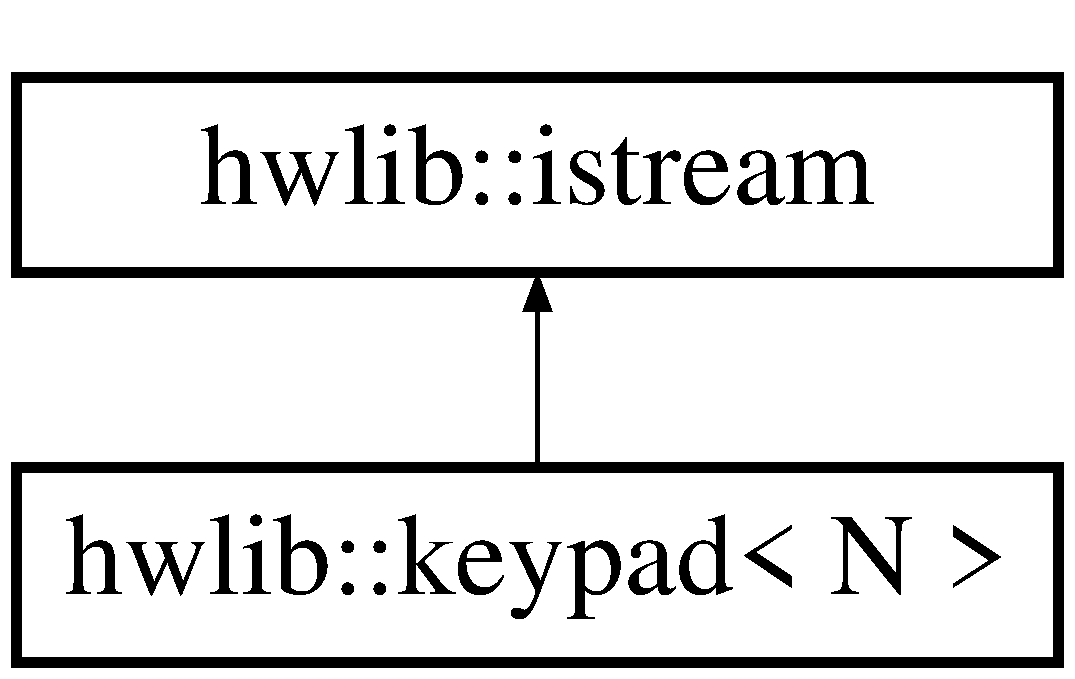
\includegraphics[height=2.000000cm]{classhwlib_1_1istream}
\end{center}
\end{figure}
\subsection*{Public Member Functions}
\begin{DoxyCompactItemize}
\item 
virtual bool \hyperlink{classhwlib_1_1istream_ad412c296e0068a518677af8cd4850e63}{char\+\_\+available} ()=0\hypertarget{classhwlib_1_1istream_ad412c296e0068a518677af8cd4850e63}{}\label{classhwlib_1_1istream_ad412c296e0068a518677af8cd4850e63}

\begin{DoxyCompactList}\small\item\em reports whether a character is available \end{DoxyCompactList}\item 
virtual char \hyperlink{classhwlib_1_1istream_a9a260f800b08d4788b9e399f65d1c728}{getc} ()=0\hypertarget{classhwlib_1_1istream_a9a260f800b08d4788b9e399f65d1c728}{}\label{classhwlib_1_1istream_a9a260f800b08d4788b9e399f65d1c728}

\begin{DoxyCompactList}\small\item\em waits for an availbe character and returns it \end{DoxyCompactList}\item 
virtual bool \hyperlink{classhwlib_1_1istream_ad412c296e0068a518677af8cd4850e63}{char\+\_\+available} ()=0\hypertarget{classhwlib_1_1istream_ad412c296e0068a518677af8cd4850e63}{}\label{classhwlib_1_1istream_ad412c296e0068a518677af8cd4850e63}

\begin{DoxyCompactList}\small\item\em reports whether a character is available \end{DoxyCompactList}\item 
virtual char \hyperlink{classhwlib_1_1istream_a9a260f800b08d4788b9e399f65d1c728}{getc} ()=0\hypertarget{classhwlib_1_1istream_a9a260f800b08d4788b9e399f65d1c728}{}\label{classhwlib_1_1istream_a9a260f800b08d4788b9e399f65d1c728}

\begin{DoxyCompactList}\small\item\em waits for an availbe character and returns it \end{DoxyCompactList}\end{DoxyCompactItemize}
\subsection*{Friends}
\begin{DoxyCompactItemize}
\item 
\hyperlink{classhwlib_1_1istream}{istream} \& \hyperlink{classhwlib_1_1istream_a88dabf0f321a5f098ede5ee108d0a92b}{operator$>$$>$} (\hyperlink{classhwlib_1_1istream}{istream} \&stream, char \&x)
\begin{DoxyCompactList}\small\item\em input operator for char \end{DoxyCompactList}\item 
\hyperlink{classhwlib_1_1istream}{istream} \& \hyperlink{classhwlib_1_1istream_a88dabf0f321a5f098ede5ee108d0a92b}{operator$>$$>$} (\hyperlink{classhwlib_1_1istream}{istream} \&stream, char \&x)
\begin{DoxyCompactList}\small\item\em input operator for char \end{DoxyCompactList}\end{DoxyCompactItemize}


\subsection{Detailed Description}
character input stream 

\subsection{Friends And Related Function Documentation}
\index{hwlib\+::istream@{hwlib\+::istream}!operator$>$$>$@{operator$>$$>$}}
\index{operator$>$$>$@{operator$>$$>$}!hwlib\+::istream@{hwlib\+::istream}}
\subsubsection[{\texorpdfstring{operator$>$$>$}{operator>>}}]{\setlength{\rightskip}{0pt plus 5cm}{\bf istream}\& operator$>$$>$ (
\begin{DoxyParamCaption}
\item[{{\bf istream} \&}]{stream, }
\item[{char \&}]{x}
\end{DoxyParamCaption}
)\hspace{0.3cm}{\ttfamily [friend]}}\hypertarget{classhwlib_1_1istream_a88dabf0f321a5f098ede5ee108d0a92b}{}\label{classhwlib_1_1istream_a88dabf0f321a5f098ede5ee108d0a92b}


input operator for char 

This operator will wait until a character is available an then assigin it to the x parameter. \index{hwlib\+::istream@{hwlib\+::istream}!operator$>$$>$@{operator$>$$>$}}
\index{operator$>$$>$@{operator$>$$>$}!hwlib\+::istream@{hwlib\+::istream}}
\subsubsection[{\texorpdfstring{operator$>$$>$}{operator>>}}]{\setlength{\rightskip}{0pt plus 5cm}{\bf istream}\& operator$>$$>$ (
\begin{DoxyParamCaption}
\item[{{\bf istream} \&}]{stream, }
\item[{char \&}]{x}
\end{DoxyParamCaption}
)\hspace{0.3cm}{\ttfamily [friend]}}\hypertarget{classhwlib_1_1istream_a88dabf0f321a5f098ede5ee108d0a92b}{}\label{classhwlib_1_1istream_a88dabf0f321a5f098ede5ee108d0a92b}


input operator for char 

This operator will wait until a character is available an then assigin it to the x parameter. 

The documentation for this class was generated from the following files\+:\begin{DoxyCompactItemize}
\item 
\hyperlink{hwlib-ostream_01-_01_copy_8hpp}{hwlib-\/ostream -\/ Copy.\+hpp}\item 
\hyperlink{hwlib-ostream_8hpp}{hwlib-\/ostream.\+hpp}\end{DoxyCompactItemize}

\hypertarget{classhwlib_1_1keypad}{}\section{hwlib\+:\+:keypad$<$ N $>$ Class Template Reference}
\label{classhwlib_1_1keypad}\index{hwlib\+::keypad$<$ N $>$@{hwlib\+::keypad$<$ N $>$}}


istream from a keaypad matrix  




{\ttfamily \#include $<$hwlib-\/matrix-\/keypad.\+hpp$>$}

Inheritance diagram for hwlib\+:\+:keypad$<$ N $>$\+:\begin{figure}[H]
\begin{center}
\leavevmode
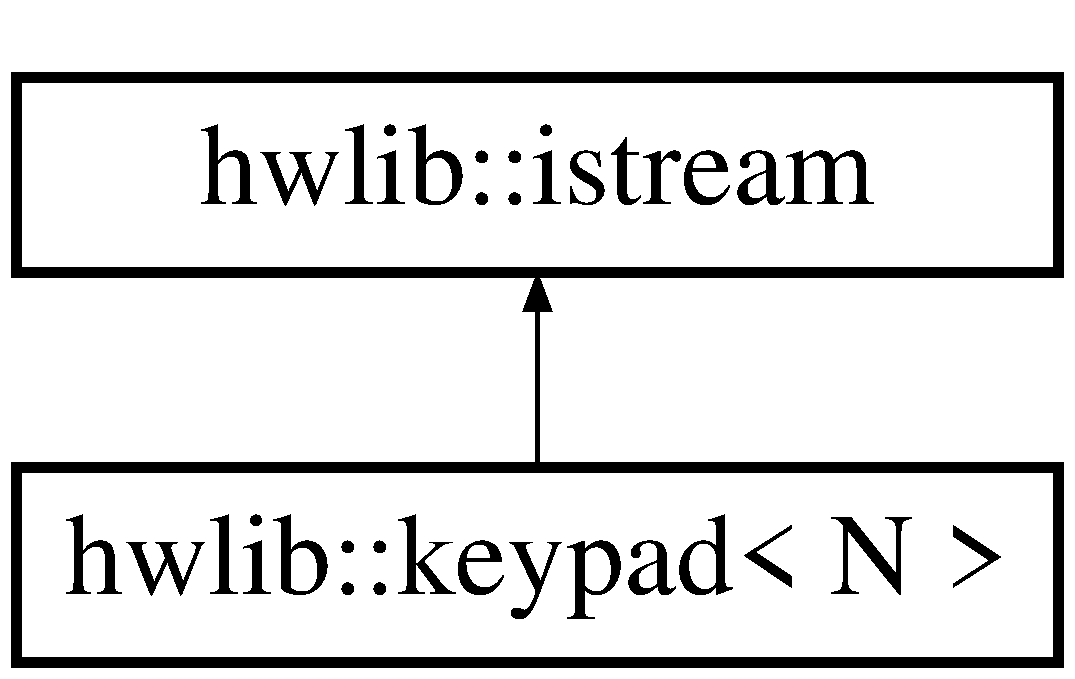
\includegraphics[height=2.000000cm]{classhwlib_1_1keypad}
\end{center}
\end{figure}
\subsection*{Public Member Functions}
\begin{DoxyCompactItemize}
\item 
\hyperlink{classhwlib_1_1keypad_a6bb965d7739192e6868a392697b6863c}{keypad} (\hyperlink{classhwlib_1_1matrix__of__switches}{matrix\+\_\+of\+\_\+switches} \&matrix, const char $\ast$translation\+\_\+string)
\begin{DoxyCompactList}\small\item\em create a keypad from a switch matrix and a translation string \end{DoxyCompactList}\item 
char \hyperlink{classhwlib_1_1keypad_a34f0f6c0cea1702e84b9f20a9379d8a8}{pressed} ()
\begin{DoxyCompactList}\small\item\em return a press character or \textquotesingle{}\textbackslash{}0\textquotesingle{} for none \end{DoxyCompactList}\item 
bool \hyperlink{classhwlib_1_1keypad_a9bef86eba2e6ac84c014a1577f44cd9c}{char\+\_\+available} () override
\begin{DoxyCompactList}\small\item\em return whether a character is available \end{DoxyCompactList}\item 
char \hyperlink{classhwlib_1_1keypad_aa2a2ab2fca1de5daa5587b3433c8e74a}{getc} () override
\begin{DoxyCompactList}\small\item\em return the next available character \end{DoxyCompactList}\end{DoxyCompactItemize}


\subsection{Detailed Description}
\subsubsection*{template$<$int N$>$\\*
class hwlib\+::keypad$<$ N $>$}

istream from a keaypad matrix 

This class template turns a keypad matrix into an istream (a character input stream). The template parameter is the number of characters in the translation string. 

\subsection{Constructor \& Destructor Documentation}
\index{hwlib\+::keypad@{hwlib\+::keypad}!keypad@{keypad}}
\index{keypad@{keypad}!hwlib\+::keypad@{hwlib\+::keypad}}
\subsubsection[{\texorpdfstring{keypad(matrix\+\_\+of\+\_\+switches \&matrix, const char $\ast$translation\+\_\+string)}{keypad(matrix_of_switches &matrix, const char *translation_string)}}]{\setlength{\rightskip}{0pt plus 5cm}template$<$int N$>$ {\bf hwlib\+::keypad}$<$ N $>$\+::{\bf keypad} (
\begin{DoxyParamCaption}
\item[{{\bf matrix\+\_\+of\+\_\+switches} \&}]{matrix, }
\item[{const char $\ast$}]{translation\+\_\+string}
\end{DoxyParamCaption}
)\hspace{0.3cm}{\ttfamily [inline]}}\hypertarget{classhwlib_1_1keypad_a6bb965d7739192e6868a392697b6863c}{}\label{classhwlib_1_1keypad_a6bb965d7739192e6868a392697b6863c}


create a keypad from a switch matrix and a translation string 

The translation string translates a pressed key to a character. The characters in the string correspond to the keys starting at the top left (1,1), proceeding colum-\/first. Excess characters in the translation string are ignored, and excess keys are translated to \textquotesingle{}\textbackslash{}0\textquotesingle{}. 

\subsection{Member Function Documentation}
\index{hwlib\+::keypad@{hwlib\+::keypad}!char\+\_\+available@{char\+\_\+available}}
\index{char\+\_\+available@{char\+\_\+available}!hwlib\+::keypad@{hwlib\+::keypad}}
\subsubsection[{\texorpdfstring{char\+\_\+available() override}{char_available() override}}]{\setlength{\rightskip}{0pt plus 5cm}template$<$int N$>$ bool {\bf hwlib\+::keypad}$<$ N $>$\+::char\+\_\+available (
\begin{DoxyParamCaption}
{}
\end{DoxyParamCaption}
)\hspace{0.3cm}{\ttfamily [inline]}, {\ttfamily [override]}, {\ttfamily [virtual]}}\hypertarget{classhwlib_1_1keypad_a9bef86eba2e6ac84c014a1577f44cd9c}{}\label{classhwlib_1_1keypad_a9bef86eba2e6ac84c014a1577f44cd9c}


return whether a character is available 

This function checks whether a next character is available. When it returns true, an (immediately) folling \hyperlink{classhwlib_1_1keypad_aa2a2ab2fca1de5daa5587b3433c8e74a}{getc()} call will not block. 

Implements \hyperlink{classhwlib_1_1istream_ad412c296e0068a518677af8cd4850e63}{hwlib\+::istream}.

\index{hwlib\+::keypad@{hwlib\+::keypad}!getc@{getc}}
\index{getc@{getc}!hwlib\+::keypad@{hwlib\+::keypad}}
\subsubsection[{\texorpdfstring{getc() override}{getc() override}}]{\setlength{\rightskip}{0pt plus 5cm}template$<$int N$>$ char {\bf hwlib\+::keypad}$<$ N $>$\+::getc (
\begin{DoxyParamCaption}
{}
\end{DoxyParamCaption}
)\hspace{0.3cm}{\ttfamily [inline]}, {\ttfamily [override]}, {\ttfamily [virtual]}}\hypertarget{classhwlib_1_1keypad_aa2a2ab2fca1de5daa5587b3433c8e74a}{}\label{classhwlib_1_1keypad_aa2a2ab2fca1de5daa5587b3433c8e74a}


return the next available character 

This function returns the next available character, if necessary it will block waiting for it. Bouncing is suppressed by checking the keypad matrix at most once every 50 ms. 

Implements \hyperlink{classhwlib_1_1istream_a9a260f800b08d4788b9e399f65d1c728}{hwlib\+::istream}.

\index{hwlib\+::keypad@{hwlib\+::keypad}!pressed@{pressed}}
\index{pressed@{pressed}!hwlib\+::keypad@{hwlib\+::keypad}}
\subsubsection[{\texorpdfstring{pressed()}{pressed()}}]{\setlength{\rightskip}{0pt plus 5cm}template$<$int N$>$ char {\bf hwlib\+::keypad}$<$ N $>$\+::pressed (
\begin{DoxyParamCaption}
{}
\end{DoxyParamCaption}
)\hspace{0.3cm}{\ttfamily [inline]}}\hypertarget{classhwlib_1_1keypad_a34f0f6c0cea1702e84b9f20a9379d8a8}{}\label{classhwlib_1_1keypad_a34f0f6c0cea1702e84b9f20a9379d8a8}


return a press character or \textquotesingle{}\textbackslash{}0\textquotesingle{} for none 

This function returns the character corresponding to a switch that is closed, or \textquotesingle{}\textbackslash{}0\textquotesingle{} when no switch is closed (or a switch is closed that has no translation). This function doesn\textquotesingle{}t suppress bouncing. 

The documentation for this class was generated from the following file\+:\begin{DoxyCompactItemize}
\item 
\hyperlink{hwlib-matrix-keypad_8hpp}{hwlib-\/matrix-\/keypad.\+hpp}\end{DoxyCompactItemize}

\hypertarget{classhwlib_1_1line}{}\section{hwlib\+:\+:line Class Reference}
\label{classhwlib_1_1line}\index{hwlib\+::line@{hwlib\+::line}}


a line object  




{\ttfamily \#include $<$hwlib-\/graphics.\+hpp$>$}

Inheritance diagram for hwlib\+:\+:line\+:\begin{figure}[H]
\begin{center}
\leavevmode
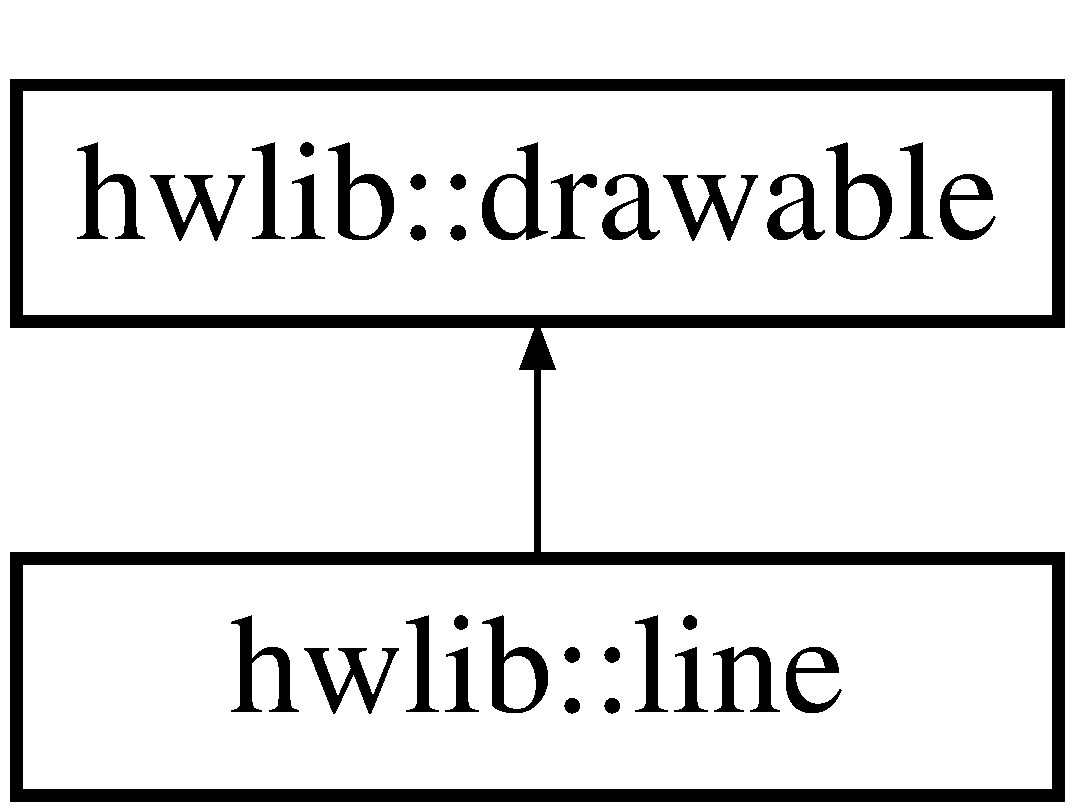
\includegraphics[height=2.000000cm]{classhwlib_1_1line}
\end{center}
\end{figure}
\subsection*{Public Member Functions}
\begin{DoxyCompactItemize}
\item 
\hyperlink{classhwlib_1_1line_a2d016ff29a2b0c6db2976651fbd40c8d}{line} (\hyperlink{classhwlib_1_1location}{location} \hyperlink{classhwlib_1_1drawable_a6c31bc9303840a4317d3c95250c357ce}{start}, \hyperlink{classhwlib_1_1location}{location} end, \hyperlink{classhwlib_1_1color}{color} fg=black)\hypertarget{classhwlib_1_1line_a2d016ff29a2b0c6db2976651fbd40c8d}{}\label{classhwlib_1_1line_a2d016ff29a2b0c6db2976651fbd40c8d}

\begin{DoxyCompactList}\small\item\em create a line object \end{DoxyCompactList}\item 
void \hyperlink{classhwlib_1_1line_a0a30c7c7e88377aada5ee1ec422bfc84}{draw} (\hyperlink{classhwlib_1_1window}{window} \&w) override\hypertarget{classhwlib_1_1line_a0a30c7c7e88377aada5ee1ec422bfc84}{}\label{classhwlib_1_1line_a0a30c7c7e88377aada5ee1ec422bfc84}

\begin{DoxyCompactList}\small\item\em interface to draw the object, you must supply the window \end{DoxyCompactList}\end{DoxyCompactItemize}
\subsection*{Additional Inherited Members}


\subsection{Detailed Description}
a line object 

The documentation for this class was generated from the following file\+:\begin{DoxyCompactItemize}
\item 
\hyperlink{hwlib-graphics_8hpp}{hwlib-\/graphics.\+hpp}\end{DoxyCompactItemize}

\hypertarget{classhwlib_1_1location}{}\section{hwlib\+:\+:location Class Reference}
\label{classhwlib_1_1location}\index{hwlib\+::location@{hwlib\+::location}}


a pixel coordinate  




{\ttfamily \#include $<$hwlib-\/graphics.\+hpp$>$}

\subsection*{Public Member Functions}
\begin{DoxyCompactItemize}
\item 
constexpr \hyperlink{classhwlib_1_1location_a773fb161de3b4b556aa85f100a0d609c}{location} (int \hyperlink{classhwlib_1_1location_abe7c9cfa19fff1fc38c9d803d0b5ce75}{x}, int \hyperlink{classhwlib_1_1location_ae8f5e3edb0ae2ec336afc6efc09f3762}{y})\hypertarget{classhwlib_1_1location_a773fb161de3b4b556aa85f100a0d609c}{}\label{classhwlib_1_1location_a773fb161de3b4b556aa85f100a0d609c}

\begin{DoxyCompactList}\small\item\em construct a location from its x and y values \end{DoxyCompactList}\item 
constexpr \hyperlink{classhwlib_1_1location}{location} \hyperlink{classhwlib_1_1location_a930b1b76ab027f12e482be4a2fc9d8ae}{operator+} (const \hyperlink{classhwlib_1_1location}{location} rhs) const \hypertarget{classhwlib_1_1location_a930b1b76ab027f12e482be4a2fc9d8ae}{}\label{classhwlib_1_1location_a930b1b76ab027f12e482be4a2fc9d8ae}

\begin{DoxyCompactList}\small\item\em add two locations \end{DoxyCompactList}\item 
constexpr \hyperlink{classhwlib_1_1location}{location} \hyperlink{classhwlib_1_1location_a4090571a5f0c80fad4b1aa8e4939ad1c}{operator-\/} (const \hyperlink{classhwlib_1_1location}{location} rhs) const \hypertarget{classhwlib_1_1location_a4090571a5f0c80fad4b1aa8e4939ad1c}{}\label{classhwlib_1_1location_a4090571a5f0c80fad4b1aa8e4939ad1c}

\begin{DoxyCompactList}\small\item\em subtract two locations \end{DoxyCompactList}\end{DoxyCompactItemize}
\subsection*{Public Attributes}
\begin{DoxyCompactItemize}
\item 
int \hyperlink{classhwlib_1_1location_abe7c9cfa19fff1fc38c9d803d0b5ce75}{x}\hypertarget{classhwlib_1_1location_abe7c9cfa19fff1fc38c9d803d0b5ce75}{}\label{classhwlib_1_1location_abe7c9cfa19fff1fc38c9d803d0b5ce75}

\begin{DoxyCompactList}\small\item\em x value of the location \end{DoxyCompactList}\item 
int \hyperlink{classhwlib_1_1location_ae8f5e3edb0ae2ec336afc6efc09f3762}{y}\hypertarget{classhwlib_1_1location_ae8f5e3edb0ae2ec336afc6efc09f3762}{}\label{classhwlib_1_1location_ae8f5e3edb0ae2ec336afc6efc09f3762}

\begin{DoxyCompactList}\small\item\em y value of the location \end{DoxyCompactList}\end{DoxyCompactItemize}


\subsection{Detailed Description}
a pixel coordinate 

This class abstracts a coordinate (pixel location) on a graphics screen, or the distance between two coordinates. 

The documentation for this class was generated from the following file\+:\begin{DoxyCompactItemize}
\item 
\hyperlink{hwlib-graphics_8hpp}{hwlib-\/graphics.\+hpp}\end{DoxyCompactItemize}

\hypertarget{classhwlib_1_1matrix__of__switches}{}\section{hwlib\+:\+:matrix\+\_\+of\+\_\+switches Class Reference}
\label{classhwlib_1_1matrix__of__switches}\index{hwlib\+::matrix\+\_\+of\+\_\+switches@{hwlib\+::matrix\+\_\+of\+\_\+switches}}


matrix of switches (keypad) interface  




{\ttfamily \#include $<$hwlib-\/matrix-\/keypad.\+hpp$>$}

\subsection*{Public Member Functions}
\begin{DoxyCompactItemize}
\item 
\hyperlink{classhwlib_1_1matrix__of__switches_a7b6df331ad1f31001ec0ab3ac51ecbc9}{matrix\+\_\+of\+\_\+switches} (\hyperlink{classhwlib_1_1port__oc}{port\+\_\+oc} \&output, \hyperlink{classhwlib_1_1port__in}{port\+\_\+in} \&input)
\begin{DoxyCompactList}\small\item\em create a matrix interface from the row and column pins \end{DoxyCompactList}\item 
bool \hyperlink{classhwlib_1_1matrix__of__switches_a6ae62c16d59ef6830a3230d52bf08f64}{switch\+\_\+is\+\_\+closed\+\_\+at} (int x, int y)
\begin{DoxyCompactList}\small\item\em test whether a particular switch is closed \end{DoxyCompactList}\end{DoxyCompactItemize}
\subsection*{Public Attributes}
\begin{DoxyCompactItemize}
\item 
const int \hyperlink{classhwlib_1_1matrix__of__switches_ab9bc5a395efdaa418d843ecfc275a081}{x\+\_\+size}\hypertarget{classhwlib_1_1matrix__of__switches_ab9bc5a395efdaa418d843ecfc275a081}{}\label{classhwlib_1_1matrix__of__switches_ab9bc5a395efdaa418d843ecfc275a081}

\begin{DoxyCompactList}\small\item\em the number of columns \end{DoxyCompactList}\item 
const int \hyperlink{classhwlib_1_1matrix__of__switches_ac87ec85080691bc41466468e95316a34}{y\+\_\+size}\hypertarget{classhwlib_1_1matrix__of__switches_ac87ec85080691bc41466468e95316a34}{}\label{classhwlib_1_1matrix__of__switches_ac87ec85080691bc41466468e95316a34}

\begin{DoxyCompactList}\small\item\em the number of rows \end{DoxyCompactList}\end{DoxyCompactItemize}


\subsection{Detailed Description}
matrix of switches (keypad) interface 

This class interfaces to a matrix of keys (switches). 

\subsection{Constructor \& Destructor Documentation}
\index{hwlib\+::matrix\+\_\+of\+\_\+switches@{hwlib\+::matrix\+\_\+of\+\_\+switches}!matrix\+\_\+of\+\_\+switches@{matrix\+\_\+of\+\_\+switches}}
\index{matrix\+\_\+of\+\_\+switches@{matrix\+\_\+of\+\_\+switches}!hwlib\+::matrix\+\_\+of\+\_\+switches@{hwlib\+::matrix\+\_\+of\+\_\+switches}}
\subsubsection[{\texorpdfstring{matrix\+\_\+of\+\_\+switches(port\+\_\+oc \&output, port\+\_\+in \&input)}{matrix_of_switches(port_oc &output, port_in &input)}}]{\setlength{\rightskip}{0pt plus 5cm}hwlib\+::matrix\+\_\+of\+\_\+switches\+::matrix\+\_\+of\+\_\+switches (
\begin{DoxyParamCaption}
\item[{{\bf port\+\_\+oc} \&}]{output, }
\item[{{\bf port\+\_\+in} \&}]{input}
\end{DoxyParamCaption}
)\hspace{0.3cm}{\ttfamily [inline]}}\hypertarget{classhwlib_1_1matrix__of__switches_a7b6df331ad1f31001ec0ab3ac51ecbc9}{}\label{classhwlib_1_1matrix__of__switches_a7b6df331ad1f31001ec0ab3ac51ecbc9}


create a matrix interface from the row and column pins 

This constructor creates a matrix interface from the ports that contain the pins that connect to the columns (x direction) and the columns (y direction). The column pins must be an open-\/collector port, the row pins muts be an input port that has (internal or external) pull-\/up resistors. 

\subsection{Member Function Documentation}
\index{hwlib\+::matrix\+\_\+of\+\_\+switches@{hwlib\+::matrix\+\_\+of\+\_\+switches}!switch\+\_\+is\+\_\+closed\+\_\+at@{switch\+\_\+is\+\_\+closed\+\_\+at}}
\index{switch\+\_\+is\+\_\+closed\+\_\+at@{switch\+\_\+is\+\_\+closed\+\_\+at}!hwlib\+::matrix\+\_\+of\+\_\+switches@{hwlib\+::matrix\+\_\+of\+\_\+switches}}
\subsubsection[{\texorpdfstring{switch\+\_\+is\+\_\+closed\+\_\+at(int x, int y)}{switch_is_closed_at(int x, int y)}}]{\setlength{\rightskip}{0pt plus 5cm}bool hwlib\+::matrix\+\_\+of\+\_\+switches\+::switch\+\_\+is\+\_\+closed\+\_\+at (
\begin{DoxyParamCaption}
\item[{int}]{x, }
\item[{int}]{y}
\end{DoxyParamCaption}
)\hspace{0.3cm}{\ttfamily [inline]}}\hypertarget{classhwlib_1_1matrix__of__switches_a6ae62c16d59ef6830a3230d52bf08f64}{}\label{classhwlib_1_1matrix__of__switches_a6ae62c16d59ef6830a3230d52bf08f64}


test whether a particular switch is closed 

This function returns whether the switch at column x and row y is closed. It doesn\textquotesingle{}t suppress bouncing. 

The documentation for this class was generated from the following file\+:\begin{DoxyCompactItemize}
\item 
\hyperlink{hwlib-matrix-keypad_8hpp}{hwlib-\/matrix-\/keypad.\+hpp}\end{DoxyCompactItemize}

\hypertarget{classhwlib_1_1ostream}{}\section{hwlib\+:\+:ostream Class Reference}
\label{classhwlib_1_1ostream}\index{hwlib\+::ostream@{hwlib\+::ostream}}


formatted character output  




{\ttfamily \#include $<$hwlib-\/ostream -\/ Copy.\+hpp$>$}

Inheritance diagram for hwlib\+:\+:ostream\+:\begin{figure}[H]
\begin{center}
\leavevmode
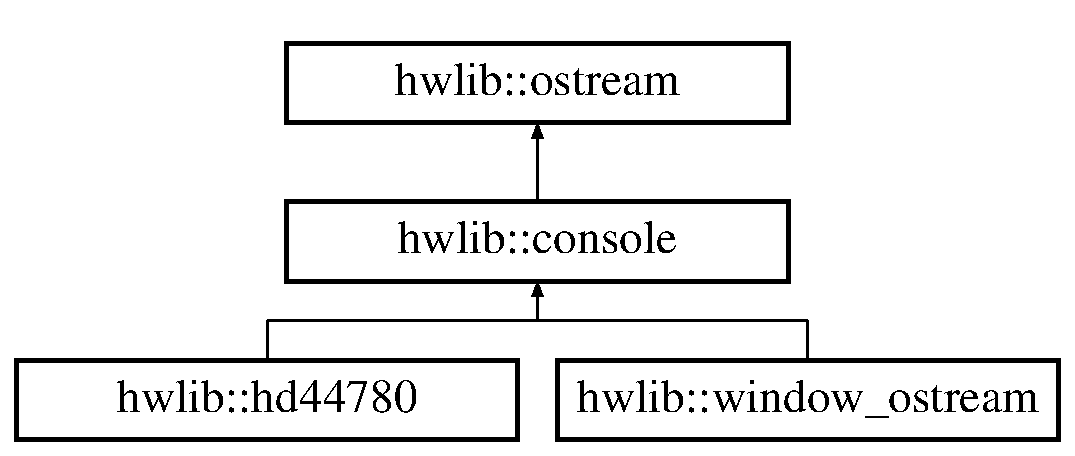
\includegraphics[height=3.000000cm]{classhwlib_1_1ostream}
\end{center}
\end{figure}
\subsection*{Public Member Functions}
\begin{DoxyCompactItemize}
\item 
virtual void \hyperlink{classhwlib_1_1ostream_a3b2b77c9e933b76bd6ddd85b9883a31b}{putc} (char c)=0
\begin{DoxyCompactList}\small\item\em char output function \end{DoxyCompactList}\item 
\hyperlink{classhwlib_1_1ostream}{ostream} \& \hyperlink{classhwlib_1_1ostream_ab7fd8d969cd3533df36944233da5c64b}{operator$<$$<$} (char c)\hypertarget{classhwlib_1_1ostream_ab7fd8d969cd3533df36944233da5c64b}{}\label{classhwlib_1_1ostream_ab7fd8d969cd3533df36944233da5c64b}

\begin{DoxyCompactList}\small\item\em char output operator \end{DoxyCompactList}\item 
virtual void \hyperlink{classhwlib_1_1ostream_ab4587e3151fc02c5faba3b06522e337f}{flush} (void)
\begin{DoxyCompactList}\small\item\em flush \end{DoxyCompactList}\item 
int \hyperlink{classhwlib_1_1ostream_aa4d58cb368e67310cd70bf9cc8579966}{width} (void) const \hypertarget{classhwlib_1_1ostream_aa4d58cb368e67310cd70bf9cc8579966}{}\label{classhwlib_1_1ostream_aa4d58cb368e67310cd70bf9cc8579966}

\begin{DoxyCompactList}\small\item\em return the current field width \end{DoxyCompactList}\item 
int \hyperlink{classhwlib_1_1ostream_a3f65c4ae6cba8d58e7f5b21f19667c0f}{width} (int x)\hypertarget{classhwlib_1_1ostream_a3f65c4ae6cba8d58e7f5b21f19667c0f}{}\label{classhwlib_1_1ostream_a3f65c4ae6cba8d58e7f5b21f19667c0f}

\begin{DoxyCompactList}\small\item\em set the field width, return the old field width \end{DoxyCompactList}\item 
int \hyperlink{classhwlib_1_1ostream_a6266f7f74a244b69c33d4c6d9be6c145}{base} (void) const \hypertarget{classhwlib_1_1ostream_a6266f7f74a244b69c33d4c6d9be6c145}{}\label{classhwlib_1_1ostream_a6266f7f74a244b69c33d4c6d9be6c145}

\begin{DoxyCompactList}\small\item\em return the numerical radix \end{DoxyCompactList}\item 
int \hyperlink{classhwlib_1_1ostream_a0895d45a31d89352d5c167dc0932399b}{base} (int x)\hypertarget{classhwlib_1_1ostream_a0895d45a31d89352d5c167dc0932399b}{}\label{classhwlib_1_1ostream_a0895d45a31d89352d5c167dc0932399b}

\begin{DoxyCompactList}\small\item\em set the numerical radix, return the old numerical radix \end{DoxyCompactList}\item 
virtual void \hyperlink{classhwlib_1_1ostream_a3b2b77c9e933b76bd6ddd85b9883a31b}{putc} (char c)=0
\begin{DoxyCompactList}\small\item\em char output function \end{DoxyCompactList}\item 
\hyperlink{classhwlib_1_1ostream}{ostream} \& \hyperlink{classhwlib_1_1ostream_ab7fd8d969cd3533df36944233da5c64b}{operator$<$$<$} (char c)\hypertarget{classhwlib_1_1ostream_ab7fd8d969cd3533df36944233da5c64b}{}\label{classhwlib_1_1ostream_ab7fd8d969cd3533df36944233da5c64b}

\begin{DoxyCompactList}\small\item\em char output operator \end{DoxyCompactList}\item 
virtual void \hyperlink{classhwlib_1_1ostream_ab4587e3151fc02c5faba3b06522e337f}{flush} (void)
\begin{DoxyCompactList}\small\item\em flush \end{DoxyCompactList}\item 
int \hyperlink{classhwlib_1_1ostream_aa4d58cb368e67310cd70bf9cc8579966}{width} (void) const \hypertarget{classhwlib_1_1ostream_aa4d58cb368e67310cd70bf9cc8579966}{}\label{classhwlib_1_1ostream_aa4d58cb368e67310cd70bf9cc8579966}

\begin{DoxyCompactList}\small\item\em return the current field width \end{DoxyCompactList}\item 
int \hyperlink{classhwlib_1_1ostream_a3f65c4ae6cba8d58e7f5b21f19667c0f}{width} (int x)\hypertarget{classhwlib_1_1ostream_a3f65c4ae6cba8d58e7f5b21f19667c0f}{}\label{classhwlib_1_1ostream_a3f65c4ae6cba8d58e7f5b21f19667c0f}

\begin{DoxyCompactList}\small\item\em set the field width, return the old field width \end{DoxyCompactList}\item 
int \hyperlink{classhwlib_1_1ostream_a6266f7f74a244b69c33d4c6d9be6c145}{base} (void) const \hypertarget{classhwlib_1_1ostream_a6266f7f74a244b69c33d4c6d9be6c145}{}\label{classhwlib_1_1ostream_a6266f7f74a244b69c33d4c6d9be6c145}

\begin{DoxyCompactList}\small\item\em return the numerical radix \end{DoxyCompactList}\item 
int \hyperlink{classhwlib_1_1ostream_a0895d45a31d89352d5c167dc0932399b}{base} (int x)\hypertarget{classhwlib_1_1ostream_a0895d45a31d89352d5c167dc0932399b}{}\label{classhwlib_1_1ostream_a0895d45a31d89352d5c167dc0932399b}

\begin{DoxyCompactList}\small\item\em set the numerical radix, return the old numerical radix \end{DoxyCompactList}\end{DoxyCompactItemize}
\subsection*{Friends}
\begin{DoxyCompactItemize}
\item 
\hyperlink{classhwlib_1_1ostream}{ostream} \& \hyperlink{classhwlib_1_1ostream_a253a2e284130cc22d3dff3fbf669afae}{operator$<$$<$} (\hyperlink{classhwlib_1_1ostream}{ostream} \&stream, bool x)\hypertarget{classhwlib_1_1ostream_a253a2e284130cc22d3dff3fbf669afae}{}\label{classhwlib_1_1ostream_a253a2e284130cc22d3dff3fbf669afae}

\begin{DoxyCompactList}\small\item\em output operator for bool \end{DoxyCompactList}\item 
\hyperlink{classhwlib_1_1ostream}{ostream} \& \hyperlink{classhwlib_1_1ostream_a45bbf00f11c411f55e5eef9b28165fa6}{operator$<$$<$} (\hyperlink{classhwlib_1_1ostream}{ostream} \&stream, const char $\ast$s)\hypertarget{classhwlib_1_1ostream_a45bbf00f11c411f55e5eef9b28165fa6}{}\label{classhwlib_1_1ostream_a45bbf00f11c411f55e5eef9b28165fa6}

\begin{DoxyCompactList}\small\item\em output operator for const char pointer (literal string) \end{DoxyCompactList}\item 
\hyperlink{classhwlib_1_1ostream}{ostream} \& \hyperlink{classhwlib_1_1ostream_a28ee741656d0ad9d6a1782823212e7d9}{operator$<$$<$} (\hyperlink{classhwlib_1_1ostream}{ostream} \&stream, int x)\hypertarget{classhwlib_1_1ostream_a28ee741656d0ad9d6a1782823212e7d9}{}\label{classhwlib_1_1ostream_a28ee741656d0ad9d6a1782823212e7d9}

\begin{DoxyCompactList}\small\item\em output operator for integer \end{DoxyCompactList}\item 
\hyperlink{classhwlib_1_1ostream}{ostream} \& \hyperlink{classhwlib_1_1ostream_a5f10f89fa98ac5e5f89cc2af0e9b0b6e}{operator$<$$<$} (\hyperlink{classhwlib_1_1ostream}{ostream} \&stream, short int x)\hypertarget{classhwlib_1_1ostream_a5f10f89fa98ac5e5f89cc2af0e9b0b6e}{}\label{classhwlib_1_1ostream_a5f10f89fa98ac5e5f89cc2af0e9b0b6e}

\begin{DoxyCompactList}\small\item\em output operator for short integer \end{DoxyCompactList}\item 
\hyperlink{classhwlib_1_1ostream}{ostream} \& \hyperlink{classhwlib_1_1ostream_af269c1256dc5c755fafc13a7b9125187}{operator$<$$<$} (\hyperlink{classhwlib_1_1ostream}{ostream} \&stream, long int x)\hypertarget{classhwlib_1_1ostream_af269c1256dc5c755fafc13a7b9125187}{}\label{classhwlib_1_1ostream_af269c1256dc5c755fafc13a7b9125187}

\begin{DoxyCompactList}\small\item\em output operator for long integer \end{DoxyCompactList}\item 
\hyperlink{classhwlib_1_1ostream}{ostream} \& \hyperlink{classhwlib_1_1ostream_a25a0b9be93f8f9ed789cef2411acbed2}{operator$<$$<$} (\hyperlink{classhwlib_1_1ostream}{ostream} \&stream, long long int x)\hypertarget{classhwlib_1_1ostream_a25a0b9be93f8f9ed789cef2411acbed2}{}\label{classhwlib_1_1ostream_a25a0b9be93f8f9ed789cef2411acbed2}

\begin{DoxyCompactList}\small\item\em output operator for long long integer \end{DoxyCompactList}\item 
\hyperlink{classhwlib_1_1ostream}{ostream} \& \hyperlink{classhwlib_1_1ostream_a2c5c3586c979f880097499e392bcbf54}{operator$<$$<$} (\hyperlink{classhwlib_1_1ostream}{ostream} \&stream, short unsigned int x)\hypertarget{classhwlib_1_1ostream_a2c5c3586c979f880097499e392bcbf54}{}\label{classhwlib_1_1ostream_a2c5c3586c979f880097499e392bcbf54}

\begin{DoxyCompactList}\small\item\em output operator for short unsigned integer \end{DoxyCompactList}\item 
\hyperlink{classhwlib_1_1ostream}{ostream} \& \hyperlink{classhwlib_1_1ostream_ae70e52926d415af7bfd483c29322f6a1}{operator$<$$<$} (\hyperlink{classhwlib_1_1ostream}{ostream} \&stream, unsigned int x)\hypertarget{classhwlib_1_1ostream_ae70e52926d415af7bfd483c29322f6a1}{}\label{classhwlib_1_1ostream_ae70e52926d415af7bfd483c29322f6a1}

\begin{DoxyCompactList}\small\item\em output operator for unsigned integer \end{DoxyCompactList}\item 
\hyperlink{classhwlib_1_1ostream}{ostream} \& \hyperlink{classhwlib_1_1ostream_a7df95ef6e7402e0238681b5a0ee1a4f6}{operator$<$$<$} (\hyperlink{classhwlib_1_1ostream}{ostream} \&stream, unsigned long int x)\hypertarget{classhwlib_1_1ostream_a7df95ef6e7402e0238681b5a0ee1a4f6}{}\label{classhwlib_1_1ostream_a7df95ef6e7402e0238681b5a0ee1a4f6}

\begin{DoxyCompactList}\small\item\em output operator for unsigned long integer \end{DoxyCompactList}\item 
\hyperlink{classhwlib_1_1ostream}{ostream} \& \hyperlink{classhwlib_1_1ostream_a7ab00ab622e0e7c42198f34597713390}{operator$<$$<$} (\hyperlink{classhwlib_1_1ostream}{ostream} \&stream, unsigned long long x)\hypertarget{classhwlib_1_1ostream_a7ab00ab622e0e7c42198f34597713390}{}\label{classhwlib_1_1ostream_a7ab00ab622e0e7c42198f34597713390}

\begin{DoxyCompactList}\small\item\em output operator for unsigned long long integer \end{DoxyCompactList}\item 
\hyperlink{classhwlib_1_1ostream}{ostream} \& \hyperlink{classhwlib_1_1ostream_a62d3d656e6a5021fc4a6aa6940b5641e}{operator$<$$<$} (\hyperlink{classhwlib_1_1ostream}{ostream} \&stream, signed char c)\hypertarget{classhwlib_1_1ostream_a62d3d656e6a5021fc4a6aa6940b5641e}{}\label{classhwlib_1_1ostream_a62d3d656e6a5021fc4a6aa6940b5641e}

\begin{DoxyCompactList}\small\item\em output operator for signed char (prints as integer) \end{DoxyCompactList}\item 
\hyperlink{classhwlib_1_1ostream}{ostream} \& \hyperlink{classhwlib_1_1ostream_a3fea1f54c018fe926d9c7ee25ebd917a}{operator$<$$<$} (\hyperlink{classhwlib_1_1ostream}{ostream} \&stream, unsigned char c)\hypertarget{classhwlib_1_1ostream_a3fea1f54c018fe926d9c7ee25ebd917a}{}\label{classhwlib_1_1ostream_a3fea1f54c018fe926d9c7ee25ebd917a}

\begin{DoxyCompactList}\small\item\em output operator for unsigned char (prints as integer) \end{DoxyCompactList}\item 
\hyperlink{classhwlib_1_1ostream}{ostream} \& \hyperlink{classhwlib_1_1ostream_a253a2e284130cc22d3dff3fbf669afae}{operator$<$$<$} (\hyperlink{classhwlib_1_1ostream}{ostream} \&stream, bool x)\hypertarget{classhwlib_1_1ostream_a253a2e284130cc22d3dff3fbf669afae}{}\label{classhwlib_1_1ostream_a253a2e284130cc22d3dff3fbf669afae}

\begin{DoxyCompactList}\small\item\em output operator for bool \end{DoxyCompactList}\item 
\hyperlink{classhwlib_1_1ostream}{ostream} \& \hyperlink{classhwlib_1_1ostream_a45bbf00f11c411f55e5eef9b28165fa6}{operator$<$$<$} (\hyperlink{classhwlib_1_1ostream}{ostream} \&stream, const char $\ast$s)\hypertarget{classhwlib_1_1ostream_a45bbf00f11c411f55e5eef9b28165fa6}{}\label{classhwlib_1_1ostream_a45bbf00f11c411f55e5eef9b28165fa6}

\begin{DoxyCompactList}\small\item\em output operator for const char pointer (literal string) \end{DoxyCompactList}\item 
\hyperlink{classhwlib_1_1ostream}{ostream} \& \hyperlink{classhwlib_1_1ostream_a28ee741656d0ad9d6a1782823212e7d9}{operator$<$$<$} (\hyperlink{classhwlib_1_1ostream}{ostream} \&stream, int x)\hypertarget{classhwlib_1_1ostream_a28ee741656d0ad9d6a1782823212e7d9}{}\label{classhwlib_1_1ostream_a28ee741656d0ad9d6a1782823212e7d9}

\begin{DoxyCompactList}\small\item\em output operator for integer \end{DoxyCompactList}\item 
\hyperlink{classhwlib_1_1ostream}{ostream} \& \hyperlink{classhwlib_1_1ostream_a5f10f89fa98ac5e5f89cc2af0e9b0b6e}{operator$<$$<$} (\hyperlink{classhwlib_1_1ostream}{ostream} \&stream, short int x)\hypertarget{classhwlib_1_1ostream_a5f10f89fa98ac5e5f89cc2af0e9b0b6e}{}\label{classhwlib_1_1ostream_a5f10f89fa98ac5e5f89cc2af0e9b0b6e}

\begin{DoxyCompactList}\small\item\em output operator for short integer \end{DoxyCompactList}\item 
\hyperlink{classhwlib_1_1ostream}{ostream} \& \hyperlink{classhwlib_1_1ostream_af269c1256dc5c755fafc13a7b9125187}{operator$<$$<$} (\hyperlink{classhwlib_1_1ostream}{ostream} \&stream, long int x)\hypertarget{classhwlib_1_1ostream_af269c1256dc5c755fafc13a7b9125187}{}\label{classhwlib_1_1ostream_af269c1256dc5c755fafc13a7b9125187}

\begin{DoxyCompactList}\small\item\em output operator for long integer \end{DoxyCompactList}\item 
\hyperlink{classhwlib_1_1ostream}{ostream} \& \hyperlink{classhwlib_1_1ostream_a25a0b9be93f8f9ed789cef2411acbed2}{operator$<$$<$} (\hyperlink{classhwlib_1_1ostream}{ostream} \&stream, long long int x)\hypertarget{classhwlib_1_1ostream_a25a0b9be93f8f9ed789cef2411acbed2}{}\label{classhwlib_1_1ostream_a25a0b9be93f8f9ed789cef2411acbed2}

\begin{DoxyCompactList}\small\item\em output operator for long long integer \end{DoxyCompactList}\item 
\hyperlink{classhwlib_1_1ostream}{ostream} \& \hyperlink{classhwlib_1_1ostream_a2c5c3586c979f880097499e392bcbf54}{operator$<$$<$} (\hyperlink{classhwlib_1_1ostream}{ostream} \&stream, short unsigned int x)\hypertarget{classhwlib_1_1ostream_a2c5c3586c979f880097499e392bcbf54}{}\label{classhwlib_1_1ostream_a2c5c3586c979f880097499e392bcbf54}

\begin{DoxyCompactList}\small\item\em output operator for short unsigned integer \end{DoxyCompactList}\item 
\hyperlink{classhwlib_1_1ostream}{ostream} \& \hyperlink{classhwlib_1_1ostream_ae70e52926d415af7bfd483c29322f6a1}{operator$<$$<$} (\hyperlink{classhwlib_1_1ostream}{ostream} \&stream, unsigned int x)\hypertarget{classhwlib_1_1ostream_ae70e52926d415af7bfd483c29322f6a1}{}\label{classhwlib_1_1ostream_ae70e52926d415af7bfd483c29322f6a1}

\begin{DoxyCompactList}\small\item\em output operator for unsigned integer \end{DoxyCompactList}\item 
\hyperlink{classhwlib_1_1ostream}{ostream} \& \hyperlink{classhwlib_1_1ostream_a7df95ef6e7402e0238681b5a0ee1a4f6}{operator$<$$<$} (\hyperlink{classhwlib_1_1ostream}{ostream} \&stream, unsigned long int x)\hypertarget{classhwlib_1_1ostream_a7df95ef6e7402e0238681b5a0ee1a4f6}{}\label{classhwlib_1_1ostream_a7df95ef6e7402e0238681b5a0ee1a4f6}

\begin{DoxyCompactList}\small\item\em output operator for unsigned long integer \end{DoxyCompactList}\item 
\hyperlink{classhwlib_1_1ostream}{ostream} \& \hyperlink{classhwlib_1_1ostream_a7ab00ab622e0e7c42198f34597713390}{operator$<$$<$} (\hyperlink{classhwlib_1_1ostream}{ostream} \&stream, unsigned long long x)\hypertarget{classhwlib_1_1ostream_a7ab00ab622e0e7c42198f34597713390}{}\label{classhwlib_1_1ostream_a7ab00ab622e0e7c42198f34597713390}

\begin{DoxyCompactList}\small\item\em output operator for unsigned long long integer \end{DoxyCompactList}\item 
\hyperlink{classhwlib_1_1ostream}{ostream} \& \hyperlink{classhwlib_1_1ostream_a62d3d656e6a5021fc4a6aa6940b5641e}{operator$<$$<$} (\hyperlink{classhwlib_1_1ostream}{ostream} \&stream, signed char c)\hypertarget{classhwlib_1_1ostream_a62d3d656e6a5021fc4a6aa6940b5641e}{}\label{classhwlib_1_1ostream_a62d3d656e6a5021fc4a6aa6940b5641e}

\begin{DoxyCompactList}\small\item\em output operator for signed char (prints as integer) \end{DoxyCompactList}\item 
\hyperlink{classhwlib_1_1ostream}{ostream} \& \hyperlink{classhwlib_1_1ostream_a3fea1f54c018fe926d9c7ee25ebd917a}{operator$<$$<$} (\hyperlink{classhwlib_1_1ostream}{ostream} \&stream, unsigned char c)\hypertarget{classhwlib_1_1ostream_a3fea1f54c018fe926d9c7ee25ebd917a}{}\label{classhwlib_1_1ostream_a3fea1f54c018fe926d9c7ee25ebd917a}

\begin{DoxyCompactList}\small\item\em output operator for unsigned char (prints as integer) \end{DoxyCompactList}\end{DoxyCompactItemize}
\subsection*{Related Functions}
(Note that these are not member functions.) \begin{DoxyCompactItemize}
\item 
bool \hyperlink{classhwlib_1_1ostream_a5b8e4c021711ab0fbbefcd2df29c03a7}{showpos} (void) const 
\begin{DoxyCompactList}\small\item\em return the current showpos setting \end{DoxyCompactList}\item 
bool \hyperlink{classhwlib_1_1ostream_a63eb8b78e5a4a3250043b4b9ecb35f16}{showpos} (bool x)
\begin{DoxyCompactList}\small\item\em set the showpos setting, return the old showpos setting \end{DoxyCompactList}\item 
bool \hyperlink{classhwlib_1_1ostream_aa47993e8c6771ed093859416133b3724}{showbase} (void) const 
\begin{DoxyCompactList}\small\item\em return the current showbase setting \end{DoxyCompactList}\item 
bool \hyperlink{classhwlib_1_1ostream_ad3290e2669fd1ced136efc657f4478a2}{showbase} (bool x)
\begin{DoxyCompactList}\small\item\em set the showbase setting, return the old showbase setting \end{DoxyCompactList}\item 
bool \hyperlink{classhwlib_1_1ostream_aa4ad6c4c344926b02b165e89bddb98b5}{boolalpha} (void) const 
\begin{DoxyCompactList}\small\item\em return the current boolalpha setting \end{DoxyCompactList}\item 
bool \hyperlink{classhwlib_1_1ostream_a4b94d035da5b074afee5fdef06dcf737}{boolalpha} (bool x)
\begin{DoxyCompactList}\small\item\em set the noboolalpha setting, return the old noboolalpha setting \end{DoxyCompactList}\item 
char \hyperlink{classhwlib_1_1ostream_a11cfd99e60bf22ace9e11c40da61d3ec}{fill} (void) const 
\begin{DoxyCompactList}\small\item\em return the current fill char setting \end{DoxyCompactList}\item 
char \hyperlink{classhwlib_1_1ostream_a7d7d3d7d7bd7896c51649a8c9c0a236c}{fill} (char x)
\begin{DoxyCompactList}\small\item\em set the fill char setting, return the old fill char setting \end{DoxyCompactList}\item 
bool \hyperlink{classhwlib_1_1ostream_a5b8e4c021711ab0fbbefcd2df29c03a7}{showpos} (void) const 
\begin{DoxyCompactList}\small\item\em return the current showpos setting \end{DoxyCompactList}\item 
bool \hyperlink{classhwlib_1_1ostream_a63eb8b78e5a4a3250043b4b9ecb35f16}{showpos} (bool x)
\begin{DoxyCompactList}\small\item\em set the showpos setting, return the old showpos setting \end{DoxyCompactList}\item 
bool \hyperlink{classhwlib_1_1ostream_aa47993e8c6771ed093859416133b3724}{showbase} (void) const 
\begin{DoxyCompactList}\small\item\em return the current showbase setting \end{DoxyCompactList}\item 
bool \hyperlink{classhwlib_1_1ostream_ad3290e2669fd1ced136efc657f4478a2}{showbase} (bool x)
\begin{DoxyCompactList}\small\item\em set the showbase setting, return the old showbase setting \end{DoxyCompactList}\item 
bool \hyperlink{classhwlib_1_1ostream_aa4ad6c4c344926b02b165e89bddb98b5}{boolalpha} (void) const 
\begin{DoxyCompactList}\small\item\em return the current boolalpha setting \end{DoxyCompactList}\item 
bool \hyperlink{classhwlib_1_1ostream_a4b94d035da5b074afee5fdef06dcf737}{boolalpha} (bool x)
\begin{DoxyCompactList}\small\item\em set the noboolalpha setting, return the old noboolalpha setting \end{DoxyCompactList}\item 
char \hyperlink{classhwlib_1_1ostream_a11cfd99e60bf22ace9e11c40da61d3ec}{fill} (void) const 
\begin{DoxyCompactList}\small\item\em return the current fill char setting \end{DoxyCompactList}\item 
char \hyperlink{classhwlib_1_1ostream_a7d7d3d7d7bd7896c51649a8c9c0a236c}{fill} (char x)
\begin{DoxyCompactList}\small\item\em set the fill char setting, return the old fill char setting \end{DoxyCompactList}\end{DoxyCompactItemize}


\subsection{Detailed Description}
formatted character output 

This class is an std\+::ostream work-\/alike for small embedded systems. Most formatting features of std\+::ostream are supported. Floating point values are not supported.

This class is abstract\+: a concrete subclass must implement \hyperlink{classhwlib_1_1ostream_a3b2b77c9e933b76bd6ddd85b9883a31b}{putc()} (and, when appropriate, \hyperlink{classhwlib_1_1ostream_ab4587e3151fc02c5faba3b06522e337f}{flush()}). 

\subsection{Member Function Documentation}
\index{hwlib\+::ostream@{hwlib\+::ostream}!flush@{flush}}
\index{flush@{flush}!hwlib\+::ostream@{hwlib\+::ostream}}
\subsubsection[{\texorpdfstring{flush(void)}{flush(void)}}]{\setlength{\rightskip}{0pt plus 5cm}virtual void hwlib\+::ostream\+::flush (
\begin{DoxyParamCaption}
\item[{void}]{}
\end{DoxyParamCaption}
)\hspace{0.3cm}{\ttfamily [inline]}, {\ttfamily [virtual]}}\hypertarget{classhwlib_1_1ostream_ab4587e3151fc02c5faba3b06522e337f}{}\label{classhwlib_1_1ostream_ab4587e3151fc02c5faba3b06522e337f}


flush 

This function waits until all characters are realy written to whatever is their destination. The default implementation assumes that no buffering is done, hence it returns immediately.

Writing the flush constant has the same effect as calling \hyperlink{classhwlib_1_1ostream_ab4587e3151fc02c5faba3b06522e337f}{flush()}. \index{hwlib\+::ostream@{hwlib\+::ostream}!flush@{flush}}
\index{flush@{flush}!hwlib\+::ostream@{hwlib\+::ostream}}
\subsubsection[{\texorpdfstring{flush(void)}{flush(void)}}]{\setlength{\rightskip}{0pt plus 5cm}virtual void hwlib\+::ostream\+::flush (
\begin{DoxyParamCaption}
\item[{void}]{}
\end{DoxyParamCaption}
)\hspace{0.3cm}{\ttfamily [inline]}, {\ttfamily [virtual]}}\hypertarget{classhwlib_1_1ostream_ab4587e3151fc02c5faba3b06522e337f}{}\label{classhwlib_1_1ostream_ab4587e3151fc02c5faba3b06522e337f}


flush 

This function waits until all characters are realy written to whatever is their destination. The default implementation assumes that no buffering is done, hence it returns immediately.

Writing the flush constant has the same effect as calling \hyperlink{classhwlib_1_1ostream_ab4587e3151fc02c5faba3b06522e337f}{flush()}. \index{hwlib\+::ostream@{hwlib\+::ostream}!putc@{putc}}
\index{putc@{putc}!hwlib\+::ostream@{hwlib\+::ostream}}
\subsubsection[{\texorpdfstring{putc(char c)=0}{putc(char c)=0}}]{\setlength{\rightskip}{0pt plus 5cm}virtual void hwlib\+::ostream\+::putc (
\begin{DoxyParamCaption}
\item[{char}]{c}
\end{DoxyParamCaption}
)\hspace{0.3cm}{\ttfamily [pure virtual]}}\hypertarget{classhwlib_1_1ostream_a3b2b77c9e933b76bd6ddd85b9883a31b}{}\label{classhwlib_1_1ostream_a3b2b77c9e933b76bd6ddd85b9883a31b}


char output function 

This function is called by the other functions to output each character. 

Implemented in \hyperlink{classhwlib_1_1console_ae265a4538a03a68a0ceadcc5fca153f4}{hwlib\+::console}.

\index{hwlib\+::ostream@{hwlib\+::ostream}!putc@{putc}}
\index{putc@{putc}!hwlib\+::ostream@{hwlib\+::ostream}}
\subsubsection[{\texorpdfstring{putc(char c)=0}{putc(char c)=0}}]{\setlength{\rightskip}{0pt plus 5cm}virtual void hwlib\+::ostream\+::putc (
\begin{DoxyParamCaption}
\item[{char}]{c}
\end{DoxyParamCaption}
)\hspace{0.3cm}{\ttfamily [pure virtual]}}\hypertarget{classhwlib_1_1ostream_a3b2b77c9e933b76bd6ddd85b9883a31b}{}\label{classhwlib_1_1ostream_a3b2b77c9e933b76bd6ddd85b9883a31b}


char output function 

This function is called by the other functions to output each character. 

Implemented in \hyperlink{classhwlib_1_1console_ae265a4538a03a68a0ceadcc5fca153f4}{hwlib\+::console}.



\subsection{Friends And Related Function Documentation}
\index{hwlib\+::ostream@{hwlib\+::ostream}!boolalpha@{boolalpha}}
\index{boolalpha@{boolalpha}!hwlib\+::ostream@{hwlib\+::ostream}}
\subsubsection[{\texorpdfstring{boolalpha(void) const }{boolalpha(void) const }}]{\setlength{\rightskip}{0pt plus 5cm}bool boolalpha (
\begin{DoxyParamCaption}
\item[{void}]{}
\end{DoxyParamCaption}
) const\hspace{0.3cm}{\ttfamily [related]}}\hypertarget{classhwlib_1_1ostream_aa4ad6c4c344926b02b165e89bddb98b5}{}\label{classhwlib_1_1ostream_aa4ad6c4c344926b02b165e89bddb98b5}


return the current boolalpha setting 

\index{hwlib\+::ostream@{hwlib\+::ostream}!boolalpha@{boolalpha}}
\index{boolalpha@{boolalpha}!hwlib\+::ostream@{hwlib\+::ostream}}
\subsubsection[{\texorpdfstring{boolalpha(void) const }{boolalpha(void) const }}]{\setlength{\rightskip}{0pt plus 5cm}bool boolalpha (
\begin{DoxyParamCaption}
\item[{void}]{}
\end{DoxyParamCaption}
) const\hspace{0.3cm}{\ttfamily [related]}}\hypertarget{classhwlib_1_1ostream_aa4ad6c4c344926b02b165e89bddb98b5}{}\label{classhwlib_1_1ostream_aa4ad6c4c344926b02b165e89bddb98b5}


return the current boolalpha setting 

\index{hwlib\+::ostream@{hwlib\+::ostream}!boolalpha@{boolalpha}}
\index{boolalpha@{boolalpha}!hwlib\+::ostream@{hwlib\+::ostream}}
\subsubsection[{\texorpdfstring{boolalpha(bool x)}{boolalpha(bool x)}}]{\setlength{\rightskip}{0pt plus 5cm}bool boolalpha (
\begin{DoxyParamCaption}
\item[{bool}]{x}
\end{DoxyParamCaption}
)\hspace{0.3cm}{\ttfamily [related]}}\hypertarget{classhwlib_1_1ostream_a4b94d035da5b074afee5fdef06dcf737}{}\label{classhwlib_1_1ostream_a4b94d035da5b074afee5fdef06dcf737}


set the noboolalpha setting, return the old noboolalpha setting 

\index{hwlib\+::ostream@{hwlib\+::ostream}!boolalpha@{boolalpha}}
\index{boolalpha@{boolalpha}!hwlib\+::ostream@{hwlib\+::ostream}}
\subsubsection[{\texorpdfstring{boolalpha(bool x)}{boolalpha(bool x)}}]{\setlength{\rightskip}{0pt plus 5cm}bool boolalpha (
\begin{DoxyParamCaption}
\item[{bool}]{x}
\end{DoxyParamCaption}
)\hspace{0.3cm}{\ttfamily [related]}}\hypertarget{classhwlib_1_1ostream_a4b94d035da5b074afee5fdef06dcf737}{}\label{classhwlib_1_1ostream_a4b94d035da5b074afee5fdef06dcf737}


set the noboolalpha setting, return the old noboolalpha setting 

\index{hwlib\+::ostream@{hwlib\+::ostream}!fill@{fill}}
\index{fill@{fill}!hwlib\+::ostream@{hwlib\+::ostream}}
\subsubsection[{\texorpdfstring{fill(void) const }{fill(void) const }}]{\setlength{\rightskip}{0pt plus 5cm}char fill (
\begin{DoxyParamCaption}
\item[{void}]{}
\end{DoxyParamCaption}
) const\hspace{0.3cm}{\ttfamily [related]}}\hypertarget{classhwlib_1_1ostream_a11cfd99e60bf22ace9e11c40da61d3ec}{}\label{classhwlib_1_1ostream_a11cfd99e60bf22ace9e11c40da61d3ec}


return the current fill char setting 

\index{hwlib\+::ostream@{hwlib\+::ostream}!fill@{fill}}
\index{fill@{fill}!hwlib\+::ostream@{hwlib\+::ostream}}
\subsubsection[{\texorpdfstring{fill(void) const }{fill(void) const }}]{\setlength{\rightskip}{0pt plus 5cm}char fill (
\begin{DoxyParamCaption}
\item[{void}]{}
\end{DoxyParamCaption}
) const\hspace{0.3cm}{\ttfamily [related]}}\hypertarget{classhwlib_1_1ostream_a11cfd99e60bf22ace9e11c40da61d3ec}{}\label{classhwlib_1_1ostream_a11cfd99e60bf22ace9e11c40da61d3ec}


return the current fill char setting 

\index{hwlib\+::ostream@{hwlib\+::ostream}!fill@{fill}}
\index{fill@{fill}!hwlib\+::ostream@{hwlib\+::ostream}}
\subsubsection[{\texorpdfstring{fill(char x)}{fill(char x)}}]{\setlength{\rightskip}{0pt plus 5cm}char fill (
\begin{DoxyParamCaption}
\item[{char}]{x}
\end{DoxyParamCaption}
)\hspace{0.3cm}{\ttfamily [related]}}\hypertarget{classhwlib_1_1ostream_a7d7d3d7d7bd7896c51649a8c9c0a236c}{}\label{classhwlib_1_1ostream_a7d7d3d7d7bd7896c51649a8c9c0a236c}


set the fill char setting, return the old fill char setting 

\index{hwlib\+::ostream@{hwlib\+::ostream}!fill@{fill}}
\index{fill@{fill}!hwlib\+::ostream@{hwlib\+::ostream}}
\subsubsection[{\texorpdfstring{fill(char x)}{fill(char x)}}]{\setlength{\rightskip}{0pt plus 5cm}char fill (
\begin{DoxyParamCaption}
\item[{char}]{x}
\end{DoxyParamCaption}
)\hspace{0.3cm}{\ttfamily [related]}}\hypertarget{classhwlib_1_1ostream_a7d7d3d7d7bd7896c51649a8c9c0a236c}{}\label{classhwlib_1_1ostream_a7d7d3d7d7bd7896c51649a8c9c0a236c}


set the fill char setting, return the old fill char setting 

\index{hwlib\+::ostream@{hwlib\+::ostream}!showbase@{showbase}}
\index{showbase@{showbase}!hwlib\+::ostream@{hwlib\+::ostream}}
\subsubsection[{\texorpdfstring{showbase(void) const }{showbase(void) const }}]{\setlength{\rightskip}{0pt plus 5cm}bool showbase (
\begin{DoxyParamCaption}
\item[{void}]{}
\end{DoxyParamCaption}
) const\hspace{0.3cm}{\ttfamily [related]}}\hypertarget{classhwlib_1_1ostream_aa47993e8c6771ed093859416133b3724}{}\label{classhwlib_1_1ostream_aa47993e8c6771ed093859416133b3724}


return the current showbase setting 

\index{hwlib\+::ostream@{hwlib\+::ostream}!showbase@{showbase}}
\index{showbase@{showbase}!hwlib\+::ostream@{hwlib\+::ostream}}
\subsubsection[{\texorpdfstring{showbase(void) const }{showbase(void) const }}]{\setlength{\rightskip}{0pt plus 5cm}bool showbase (
\begin{DoxyParamCaption}
\item[{void}]{}
\end{DoxyParamCaption}
) const\hspace{0.3cm}{\ttfamily [related]}}\hypertarget{classhwlib_1_1ostream_aa47993e8c6771ed093859416133b3724}{}\label{classhwlib_1_1ostream_aa47993e8c6771ed093859416133b3724}


return the current showbase setting 

\index{hwlib\+::ostream@{hwlib\+::ostream}!showbase@{showbase}}
\index{showbase@{showbase}!hwlib\+::ostream@{hwlib\+::ostream}}
\subsubsection[{\texorpdfstring{showbase(bool x)}{showbase(bool x)}}]{\setlength{\rightskip}{0pt plus 5cm}bool showbase (
\begin{DoxyParamCaption}
\item[{bool}]{x}
\end{DoxyParamCaption}
)\hspace{0.3cm}{\ttfamily [related]}}\hypertarget{classhwlib_1_1ostream_ad3290e2669fd1ced136efc657f4478a2}{}\label{classhwlib_1_1ostream_ad3290e2669fd1ced136efc657f4478a2}


set the showbase setting, return the old showbase setting 

\index{hwlib\+::ostream@{hwlib\+::ostream}!showbase@{showbase}}
\index{showbase@{showbase}!hwlib\+::ostream@{hwlib\+::ostream}}
\subsubsection[{\texorpdfstring{showbase(bool x)}{showbase(bool x)}}]{\setlength{\rightskip}{0pt plus 5cm}bool showbase (
\begin{DoxyParamCaption}
\item[{bool}]{x}
\end{DoxyParamCaption}
)\hspace{0.3cm}{\ttfamily [related]}}\hypertarget{classhwlib_1_1ostream_ad3290e2669fd1ced136efc657f4478a2}{}\label{classhwlib_1_1ostream_ad3290e2669fd1ced136efc657f4478a2}


set the showbase setting, return the old showbase setting 

\index{hwlib\+::ostream@{hwlib\+::ostream}!showpos@{showpos}}
\index{showpos@{showpos}!hwlib\+::ostream@{hwlib\+::ostream}}
\subsubsection[{\texorpdfstring{showpos(void) const }{showpos(void) const }}]{\setlength{\rightskip}{0pt plus 5cm}bool showpos (
\begin{DoxyParamCaption}
\item[{void}]{}
\end{DoxyParamCaption}
) const\hspace{0.3cm}{\ttfamily [related]}}\hypertarget{classhwlib_1_1ostream_a5b8e4c021711ab0fbbefcd2df29c03a7}{}\label{classhwlib_1_1ostream_a5b8e4c021711ab0fbbefcd2df29c03a7}


return the current showpos setting 

\index{hwlib\+::ostream@{hwlib\+::ostream}!showpos@{showpos}}
\index{showpos@{showpos}!hwlib\+::ostream@{hwlib\+::ostream}}
\subsubsection[{\texorpdfstring{showpos(void) const }{showpos(void) const }}]{\setlength{\rightskip}{0pt plus 5cm}bool showpos (
\begin{DoxyParamCaption}
\item[{void}]{}
\end{DoxyParamCaption}
) const\hspace{0.3cm}{\ttfamily [related]}}\hypertarget{classhwlib_1_1ostream_a5b8e4c021711ab0fbbefcd2df29c03a7}{}\label{classhwlib_1_1ostream_a5b8e4c021711ab0fbbefcd2df29c03a7}


return the current showpos setting 

\index{hwlib\+::ostream@{hwlib\+::ostream}!showpos@{showpos}}
\index{showpos@{showpos}!hwlib\+::ostream@{hwlib\+::ostream}}
\subsubsection[{\texorpdfstring{showpos(bool x)}{showpos(bool x)}}]{\setlength{\rightskip}{0pt plus 5cm}bool showpos (
\begin{DoxyParamCaption}
\item[{bool}]{x}
\end{DoxyParamCaption}
)\hspace{0.3cm}{\ttfamily [related]}}\hypertarget{classhwlib_1_1ostream_a63eb8b78e5a4a3250043b4b9ecb35f16}{}\label{classhwlib_1_1ostream_a63eb8b78e5a4a3250043b4b9ecb35f16}


set the showpos setting, return the old showpos setting 

\index{hwlib\+::ostream@{hwlib\+::ostream}!showpos@{showpos}}
\index{showpos@{showpos}!hwlib\+::ostream@{hwlib\+::ostream}}
\subsubsection[{\texorpdfstring{showpos(bool x)}{showpos(bool x)}}]{\setlength{\rightskip}{0pt plus 5cm}bool showpos (
\begin{DoxyParamCaption}
\item[{bool}]{x}
\end{DoxyParamCaption}
)\hspace{0.3cm}{\ttfamily [related]}}\hypertarget{classhwlib_1_1ostream_a63eb8b78e5a4a3250043b4b9ecb35f16}{}\label{classhwlib_1_1ostream_a63eb8b78e5a4a3250043b4b9ecb35f16}


set the showpos setting, return the old showpos setting 



The documentation for this class was generated from the following files\+:\begin{DoxyCompactItemize}
\item 
\hyperlink{hwlib-ostream_01-_01_copy_8hpp}{hwlib-\/ostream -\/ Copy.\+hpp}\item 
\hyperlink{hwlib-ostream_8hpp}{hwlib-\/ostream.\+hpp}\end{DoxyCompactItemize}

\hypertarget{classhwlib_1_1pcf8574a}{}\section{hwlib\+:\+:pcf8574a Class Reference}
\label{classhwlib_1_1pcf8574a}\index{hwlib\+::pcf8574a@{hwlib\+::pcf8574a}}


\hyperlink{classhwlib_1_1pcf8574a}{pcf8574a} I2C I/O extender  




{\ttfamily \#include $<$hwlib-\/pcf8574a.\+hpp$>$}

Inheritance diagram for hwlib\+:\+:pcf8574a\+:\begin{figure}[H]
\begin{center}
\leavevmode
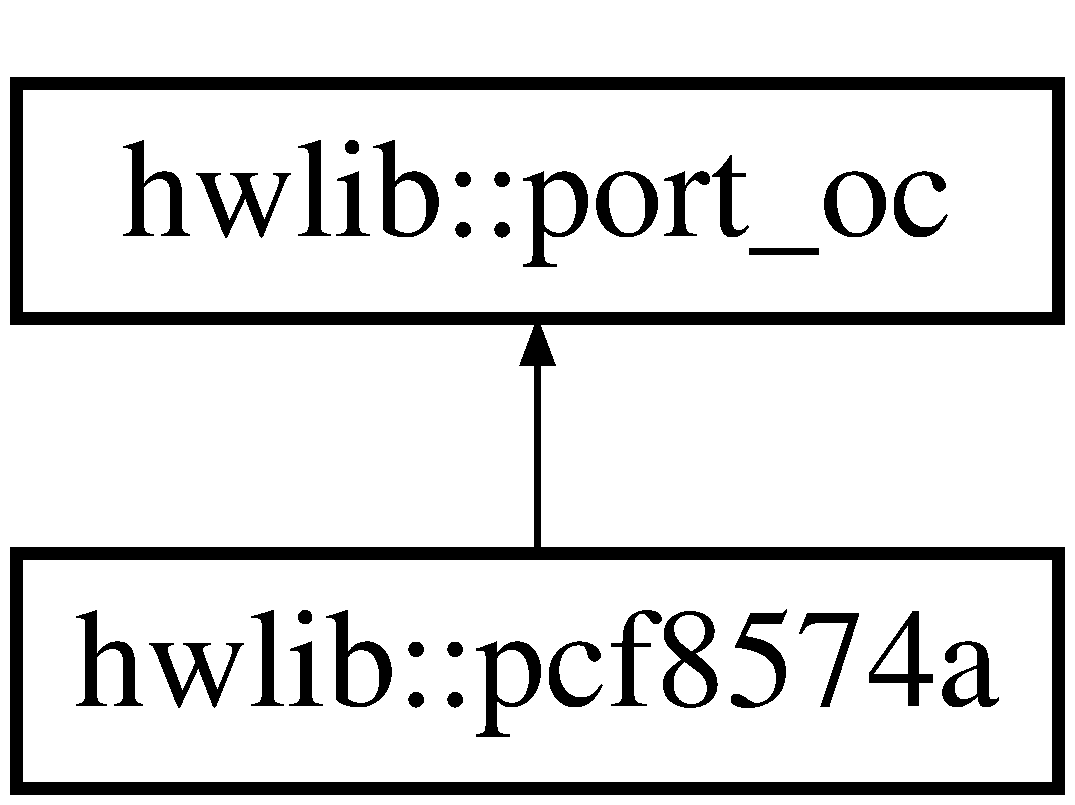
\includegraphics[height=2.000000cm]{classhwlib_1_1pcf8574a}
\end{center}
\end{figure}
\subsection*{Public Types}
\begin{DoxyCompactItemize}
\item 
typedef \+\_\+one\+\_\+pin {\bfseries one\+\_\+pin}\hypertarget{classhwlib_1_1pcf8574a_a626b4018d37bde301afe4cfa2e21cd2e}{}\label{classhwlib_1_1pcf8574a_a626b4018d37bde301afe4cfa2e21cd2e}

\end{DoxyCompactItemize}
\subsection*{Public Member Functions}
\begin{DoxyCompactItemize}
\item 
\hyperlink{classhwlib_1_1pcf8574a_abbfb14e05ed1afe9915353028264dc7b}{pcf8574a} (\hyperlink{classhwlib_1_1i2c__bus}{i2c\+\_\+bus} \&bus, \hyperlink{hwlib-defines_8hpp_a54998f25522db04b7b797b0fcc9eb3d5}{fast\+\_\+byte} address)
\begin{DoxyCompactList}\small\item\em construct an interface to a \hyperlink{classhwlib_1_1pcf8574a}{pcf8574a} chip \end{DoxyCompactList}\item 
uint\+\_\+fast8\+\_\+t \hyperlink{classhwlib_1_1pcf8574a_a1bb2266c127d93fd1d7c0b3f9193817d}{number\+\_\+of\+\_\+pins} () override
\begin{DoxyCompactList}\small\item\em get number of pins \end{DoxyCompactList}\item 
void \hyperlink{classhwlib_1_1pcf8574a_afeef7665cd9059959588295418c57709}{set} (uint\+\_\+fast8\+\_\+t x) override
\begin{DoxyCompactList}\small\item\em write to the port \end{DoxyCompactList}\item 
uint\+\_\+fast8\+\_\+t \hyperlink{classhwlib_1_1pcf8574a_abd2c5f791eced2e91f52db767351f0bd}{get} () override
\begin{DoxyCompactList}\small\item\em read from the port \end{DoxyCompactList}\end{DoxyCompactItemize}
\subsection*{Public Attributes}
{\bf }\par
\begin{DoxyCompactItemize}
\item 
one\+\_\+pin \hyperlink{classhwlib_1_1pcf8574a_a3824ca4c8ff662663dba2abf10a4a946}{p0} \{ $\ast$this, 0 \}
\begin{DoxyCompactList}\small\item\em the open-\/collector pins of the chip \end{DoxyCompactList}\item 
one\+\_\+pin {\bfseries p1} \{ $\ast$this, 1 \}\hypertarget{classhwlib_1_1pcf8574a_a1adc6413e58a9b827fa996402b18eff7}{}\label{classhwlib_1_1pcf8574a_a1adc6413e58a9b827fa996402b18eff7}

\item 
one\+\_\+pin {\bfseries p2} \{ $\ast$this, 2 \}\hypertarget{classhwlib_1_1pcf8574a_a73d8c9cd3688de0e3e7fd5cb58b9a2bd}{}\label{classhwlib_1_1pcf8574a_a73d8c9cd3688de0e3e7fd5cb58b9a2bd}

\item 
one\+\_\+pin {\bfseries p3} \{ $\ast$this, 3 \}\hypertarget{classhwlib_1_1pcf8574a_af74d66fd9f15618691755b2a9df5e7e7}{}\label{classhwlib_1_1pcf8574a_af74d66fd9f15618691755b2a9df5e7e7}

\item 
one\+\_\+pin {\bfseries p4} \{ $\ast$this, 4 \}\hypertarget{classhwlib_1_1pcf8574a_aa92b5eb9c4662e8693e481e70df36dee}{}\label{classhwlib_1_1pcf8574a_aa92b5eb9c4662e8693e481e70df36dee}

\item 
one\+\_\+pin {\bfseries p5} \{ $\ast$this, 5 \}\hypertarget{classhwlib_1_1pcf8574a_a1ee5d90ff44bc9ecd36be9a0c631a8be}{}\label{classhwlib_1_1pcf8574a_a1ee5d90ff44bc9ecd36be9a0c631a8be}

\item 
one\+\_\+pin {\bfseries p6} \{ $\ast$this, 6 \}\hypertarget{classhwlib_1_1pcf8574a_a4702f96da190fda4a82fd5c618c5adad}{}\label{classhwlib_1_1pcf8574a_a4702f96da190fda4a82fd5c618c5adad}

\item 
one\+\_\+pin {\bfseries p7} \{ $\ast$this, 7 \}\hypertarget{classhwlib_1_1pcf8574a_a57afc965233d2989de8dc9c51fa5faf5}{}\label{classhwlib_1_1pcf8574a_a57afc965233d2989de8dc9c51fa5faf5}

\end{DoxyCompactItemize}



\subsection{Detailed Description}
\hyperlink{classhwlib_1_1pcf8574a}{pcf8574a} I2C I/O extender 

This class implements an interface to a \hyperlink{classhwlib_1_1pcf8574a}{pcf8574a} I2C I/O extender chip.



A \hyperlink{classhwlib_1_1pcf8574a}{pcf8574a} is an I2C slave that provides 8 open-\/collector input/output pins with weak pull-\/ups. The power supply range is 2.\+5 .. 5.\+5 Volt. Of the 7-\/bit slave address, 3 bits are set by the level of 3 input pins (A0..A2) of the chip.



The chip has only one register, which can be read and written. When written, it determines the level of the 8 output pins\+: low when the bit is 0, pulled weakly high when the bit is 1. When read, the level of the 8 pins determines the value\+: 0 for a low pin, 1 for a high pin.

 The pcf8574 (without the -\/a) is the same chip, but with a different I2C bus address.



references\+:
\begin{DoxyItemize}
\item \href{http://www.nxp.com/documents/data_sheet/PCF8574_PCF8574A.pdf}{\tt P\+C\+F8574A data sheet} (pdf) 
\end{DoxyItemize}

\subsection{Constructor \& Destructor Documentation}
\index{hwlib\+::pcf8574a@{hwlib\+::pcf8574a}!pcf8574a@{pcf8574a}}
\index{pcf8574a@{pcf8574a}!hwlib\+::pcf8574a@{hwlib\+::pcf8574a}}
\subsubsection[{\texorpdfstring{pcf8574a(i2c\+\_\+bus \&bus, fast\+\_\+byte address)}{pcf8574a(i2c_bus &bus, fast_byte address)}}]{\setlength{\rightskip}{0pt plus 5cm}hwlib\+::pcf8574a\+::pcf8574a (
\begin{DoxyParamCaption}
\item[{{\bf i2c\+\_\+bus} \&}]{bus, }
\item[{{\bf fast\+\_\+byte}}]{address}
\end{DoxyParamCaption}
)\hspace{0.3cm}{\ttfamily [inline]}}\hypertarget{classhwlib_1_1pcf8574a_abbfb14e05ed1afe9915353028264dc7b}{}\label{classhwlib_1_1pcf8574a_abbfb14e05ed1afe9915353028264dc7b}


construct an interface to a \hyperlink{classhwlib_1_1pcf8574a}{pcf8574a} chip 

This constructor creates an interface to a \hyperlink{classhwlib_1_1pcf8574a}{pcf8574a} I2C I/O extender chip from the I2C bus it is connected to and and the chip address. The address is the 3-\/bit address that is determined by the 3 address input pins of the chip. 

\subsection{Member Function Documentation}
\index{hwlib\+::pcf8574a@{hwlib\+::pcf8574a}!get@{get}}
\index{get@{get}!hwlib\+::pcf8574a@{hwlib\+::pcf8574a}}
\subsubsection[{\texorpdfstring{get() override}{get() override}}]{\setlength{\rightskip}{0pt plus 5cm}uint\+\_\+fast8\+\_\+t hwlib\+::pcf8574a\+::get (
\begin{DoxyParamCaption}
{}
\end{DoxyParamCaption}
)\hspace{0.3cm}{\ttfamily [inline]}, {\ttfamily [override]}, {\ttfamily [virtual]}}\hypertarget{classhwlib_1_1pcf8574a_abd2c5f791eced2e91f52db767351f0bd}{}\label{classhwlib_1_1pcf8574a_abd2c5f791eced2e91f52db767351f0bd}


read from the port 

This function reads and returns the pins that are part of the port. The lowest bit of the result reflects the first pin of the port, etc.

Pins that have been written as 0 will very likley read as 0 too. To read the external input to a pin, the pin must first be written as 1. 

Implements \hyperlink{classhwlib_1_1port__oc_a49f8413dcdc6d9a172c2d9669a2e906e}{hwlib\+::port\+\_\+oc}.

\index{hwlib\+::pcf8574a@{hwlib\+::pcf8574a}!number\+\_\+of\+\_\+pins@{number\+\_\+of\+\_\+pins}}
\index{number\+\_\+of\+\_\+pins@{number\+\_\+of\+\_\+pins}!hwlib\+::pcf8574a@{hwlib\+::pcf8574a}}
\subsubsection[{\texorpdfstring{number\+\_\+of\+\_\+pins() override}{number_of_pins() override}}]{\setlength{\rightskip}{0pt plus 5cm}uint\+\_\+fast8\+\_\+t hwlib\+::pcf8574a\+::number\+\_\+of\+\_\+pins (
\begin{DoxyParamCaption}
{}
\end{DoxyParamCaption}
)\hspace{0.3cm}{\ttfamily [inline]}, {\ttfamily [override]}, {\ttfamily [virtual]}}\hypertarget{classhwlib_1_1pcf8574a_a1bb2266c127d93fd1d7c0b3f9193817d}{}\label{classhwlib_1_1pcf8574a_a1bb2266c127d93fd1d7c0b3f9193817d}


get number of pins 

This function returns the number of pins in the port. 

Implements \hyperlink{classhwlib_1_1port__oc_a44d0dbfde290ad17237ad70c09a4c402}{hwlib\+::port\+\_\+oc}.

\index{hwlib\+::pcf8574a@{hwlib\+::pcf8574a}!set@{set}}
\index{set@{set}!hwlib\+::pcf8574a@{hwlib\+::pcf8574a}}
\subsubsection[{\texorpdfstring{set(uint\+\_\+fast8\+\_\+t x) override}{set(uint_fast8_t x) override}}]{\setlength{\rightskip}{0pt plus 5cm}void hwlib\+::pcf8574a\+::set (
\begin{DoxyParamCaption}
\item[{uint\+\_\+fast8\+\_\+t}]{x}
\end{DoxyParamCaption}
)\hspace{0.3cm}{\ttfamily [inline]}, {\ttfamily [override]}, {\ttfamily [virtual]}}\hypertarget{classhwlib_1_1pcf8574a_afeef7665cd9059959588295418c57709}{}\label{classhwlib_1_1pcf8574a_afeef7665cd9059959588295418c57709}


write to the port 

This function writes to the pins that are part of the port. The lowest bit is written to the first pin of the port, etc. 

Implements \hyperlink{classhwlib_1_1port__oc_aefb3d093331e5a87cf2dbe8226dc94ef}{hwlib\+::port\+\_\+oc}.



\subsection{Member Data Documentation}
\index{hwlib\+::pcf8574a@{hwlib\+::pcf8574a}!p0@{p0}}
\index{p0@{p0}!hwlib\+::pcf8574a@{hwlib\+::pcf8574a}}
\subsubsection[{\texorpdfstring{p0}{p0}}]{\setlength{\rightskip}{0pt plus 5cm}one\+\_\+pin hwlib\+::pcf8574a\+::p0 \{ $\ast$this, 0 \}}\hypertarget{classhwlib_1_1pcf8574a_a3824ca4c8ff662663dba2abf10a4a946}{}\label{classhwlib_1_1pcf8574a_a3824ca4c8ff662663dba2abf10a4a946}


the open-\/collector pins of the chip 

The p0 ... p7 attributes represent the 8 open-\/collector output pins of the chip. A write to one of these pins will affect (only) the corresponding output pin of the chip. A read of one of these pins will reflect the status of the corresponding pin of the chip. 

The documentation for this class was generated from the following file\+:\begin{DoxyCompactItemize}
\item 
\hyperlink{hwlib-pcf8574a_8hpp}{hwlib-\/pcf8574a.\+hpp}\end{DoxyCompactItemize}

\hypertarget{classhwlib_1_1pcf8591}{}\section{hwlib\+:\+:pcf8591 Class Reference}
\label{classhwlib_1_1pcf8591}\index{hwlib\+::pcf8591@{hwlib\+::pcf8591}}


\hyperlink{classhwlib_1_1pcf8591}{pcf8591} I2C A/D and D/A converter  




{\ttfamily \#include $<$hwlib-\/pcf8591.\+hpp$>$}

\subsection*{Public Member Functions}
\begin{DoxyCompactItemize}
\item 
\hyperlink{classhwlib_1_1pcf8591_a0675613426b471f4dfcd74e83a4421b6}{pcf8591} (\hyperlink{classhwlib_1_1i2c__bus}{i2c\+\_\+bus} \&bus, \hyperlink{hwlib-defines_8hpp_a54998f25522db04b7b797b0fcc9eb3d5}{fast\+\_\+byte} address)
\begin{DoxyCompactList}\small\item\em construct an interface to a \hyperlink{classhwlib_1_1pcf8591}{pcf8591} chip \end{DoxyCompactList}\end{DoxyCompactItemize}
\subsection*{Public Attributes}
\begin{DoxyCompactItemize}
\item 
one\+\_\+dac \hyperlink{classhwlib_1_1pcf8591_a49118bd1d284d0e72aca58558b854b2d}{dac0} \{ $\ast$this \}\hypertarget{classhwlib_1_1pcf8591_a49118bd1d284d0e72aca58558b854b2d}{}\label{classhwlib_1_1pcf8591_a49118bd1d284d0e72aca58558b854b2d}

\begin{DoxyCompactList}\small\item\em the D/A converter channel of the chip \end{DoxyCompactList}\end{DoxyCompactItemize}
{\bf }\par
\begin{DoxyCompactItemize}
\item 
one\+\_\+adc \hyperlink{classhwlib_1_1pcf8591_a29a87f5711fbbd85ed5c477a5eab1b6f}{adc0} \{ $\ast$this, 0 \}
\begin{DoxyCompactList}\small\item\em the A/D converter channels of the chip \end{DoxyCompactList}\item 
one\+\_\+adc {\bfseries adc1} \{ $\ast$this, 1 \}\hypertarget{classhwlib_1_1pcf8591_aa916285265761457b7c95207d2b41118}{}\label{classhwlib_1_1pcf8591_aa916285265761457b7c95207d2b41118}

\item 
one\+\_\+adc {\bfseries adc2} \{ $\ast$this, 2 \}\hypertarget{classhwlib_1_1pcf8591_acb459e70a386e9b62fb0680ea5e84cfb}{}\label{classhwlib_1_1pcf8591_acb459e70a386e9b62fb0680ea5e84cfb}

\item 
one\+\_\+adc {\bfseries adc3} \{ $\ast$this, 3 \}\hypertarget{classhwlib_1_1pcf8591_aa89be33b4b8d5a329120e867e8d8245f}{}\label{classhwlib_1_1pcf8591_aa89be33b4b8d5a329120e867e8d8245f}

\end{DoxyCompactItemize}



\subsection{Detailed Description}
\hyperlink{classhwlib_1_1pcf8591}{pcf8591} I2C A/D and D/A converter 

This class implements an interface to a \hyperlink{classhwlib_1_1pcf8591}{pcf8591} A/D \& D/A converter chip.



A \hyperlink{classhwlib_1_1pcf8591}{pcf8591} is an I2C slave that provides 4 8-\/bits A/D inputs (that can be arranged in various combinations of single and balaced inputs), and a single8-\/bits D/A output. The power supply range is 2.\+5 .. 5.\+5 Volt. Of the 7-\/bit slave address, 3 bits are set by the level of 3 input pins (A0..A2) of the chip. references\+:
\begin{DoxyItemize}
\item \href{http://www.nxp.com/documents/data_sheet/PCF8591.pdf}{\tt P\+C\+F8591 data sheet} (pdf) 
\end{DoxyItemize}

\subsection{Constructor \& Destructor Documentation}
\index{hwlib\+::pcf8591@{hwlib\+::pcf8591}!pcf8591@{pcf8591}}
\index{pcf8591@{pcf8591}!hwlib\+::pcf8591@{hwlib\+::pcf8591}}
\subsubsection[{\texorpdfstring{pcf8591(i2c\+\_\+bus \&bus, fast\+\_\+byte address)}{pcf8591(i2c_bus &bus, fast_byte address)}}]{\setlength{\rightskip}{0pt plus 5cm}hwlib\+::pcf8591\+::pcf8591 (
\begin{DoxyParamCaption}
\item[{{\bf i2c\+\_\+bus} \&}]{bus, }
\item[{{\bf fast\+\_\+byte}}]{address}
\end{DoxyParamCaption}
)\hspace{0.3cm}{\ttfamily [inline]}}\hypertarget{classhwlib_1_1pcf8591_a0675613426b471f4dfcd74e83a4421b6}{}\label{classhwlib_1_1pcf8591_a0675613426b471f4dfcd74e83a4421b6}


construct an interface to a \hyperlink{classhwlib_1_1pcf8591}{pcf8591} chip 

This constructor creates an interface to a \hyperlink{classhwlib_1_1pcf8591}{pcf8591} I2C A/D and D/A converter from the I2C bus it is connected to and and the chip address. The address is the 3-\/bit address that is determined by the 3 address input pins of the chip. 

\subsection{Member Data Documentation}
\index{hwlib\+::pcf8591@{hwlib\+::pcf8591}!adc0@{adc0}}
\index{adc0@{adc0}!hwlib\+::pcf8591@{hwlib\+::pcf8591}}
\subsubsection[{\texorpdfstring{adc0}{adc0}}]{\setlength{\rightskip}{0pt plus 5cm}one\+\_\+adc hwlib\+::pcf8591\+::adc0 \{ $\ast$this, 0 \}}\hypertarget{classhwlib_1_1pcf8591_a29a87f5711fbbd85ed5c477a5eab1b6f}{}\label{classhwlib_1_1pcf8591_a29a87f5711fbbd85ed5c477a5eab1b6f}


the A/D converter channels of the chip 

The adc0 ... adc3 attributes represent the 4 A/D inputs of the chip. 

The documentation for this class was generated from the following file\+:\begin{DoxyCompactItemize}
\item 
\hyperlink{hwlib-pcf8591_8hpp}{hwlib-\/pcf8591.\+hpp}\end{DoxyCompactItemize}

\hypertarget{classdue_1_1pin__adc}{}\section{due\+:\+:pin\+\_\+adc Class Reference}
\label{classdue_1_1pin__adc}\index{due\+::pin\+\_\+adc@{due\+::pin\+\_\+adc}}


\hyperlink{classdue_1_1pin__adc}{pin\+\_\+adc} implementation for a A\+T\+S\+A\+M3\+X8E  




{\ttfamily \#include $<$hwlib-\/due.\+hpp$>$}

Inheritance diagram for due\+:\+:pin\+\_\+adc\+:\begin{figure}[H]
\begin{center}
\leavevmode
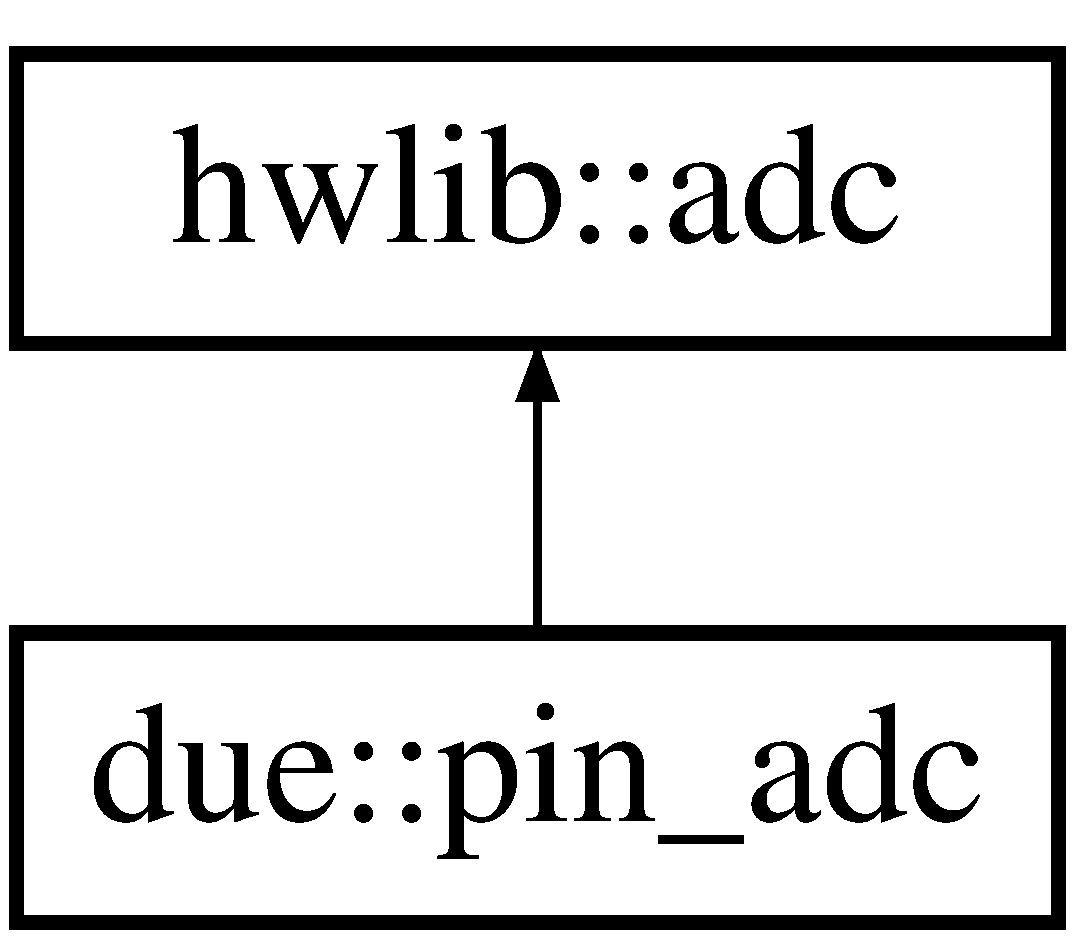
\includegraphics[height=2.000000cm]{classdue_1_1pin__adc}
\end{center}
\end{figure}
\subsection*{Public Member Functions}
\begin{DoxyCompactItemize}
\item 
\hyperlink{classdue_1_1pin__adc_a3b84a29f1ff159f40361ed969a1c8dd2}{pin\+\_\+adc} (int channel)
\begin{DoxyCompactList}\small\item\em Constructor for a A\+T\+S\+A\+M3\+X8E AD channel number. \end{DoxyCompactList}\item 
\hyperlink{classdue_1_1pin__adc_a106bc97a20bb90be8cc0d8d9152d201f}{pin\+\_\+adc} (\hyperlink{namespacedue_a5ecc98d40585c91eabbfb14f71bd7d4c}{ad\+\_\+pins} name)
\begin{DoxyCompactList}\small\item\em Arduino Due \hyperlink{classdue_1_1pin__adc}{pin\+\_\+adc} constructor from a Due pin name. \end{DoxyCompactList}\item 
\hyperlink{classhwlib_1_1adc_a7ce65f485597a481a518a4b84073605f}{adc\+\_\+value\+\_\+type} \hyperlink{classdue_1_1pin__adc_a024c090f8d9f0de7a3414d1d3dfe33d9}{get} () override
\begin{DoxyCompactList}\small\item\em get an adc reading \end{DoxyCompactList}\end{DoxyCompactItemize}
\subsection*{Additional Inherited Members}


\subsection{Detailed Description}
\hyperlink{classdue_1_1pin__adc}{pin\+\_\+adc} implementation for a A\+T\+S\+A\+M3\+X8E 

\subsection{Constructor \& Destructor Documentation}
\index{due\+::pin\+\_\+adc@{due\+::pin\+\_\+adc}!pin\+\_\+adc@{pin\+\_\+adc}}
\index{pin\+\_\+adc@{pin\+\_\+adc}!due\+::pin\+\_\+adc@{due\+::pin\+\_\+adc}}
\subsubsection[{\texorpdfstring{pin\+\_\+adc(int channel)}{pin_adc(int channel)}}]{\setlength{\rightskip}{0pt plus 5cm}due\+::pin\+\_\+adc\+::pin\+\_\+adc (
\begin{DoxyParamCaption}
\item[{int}]{channel}
\end{DoxyParamCaption}
)\hspace{0.3cm}{\ttfamily [inline]}}\hypertarget{classdue_1_1pin__adc_a3b84a29f1ff159f40361ed969a1c8dd2}{}\label{classdue_1_1pin__adc_a3b84a29f1ff159f40361ed969a1c8dd2}


Constructor for a A\+T\+S\+A\+M3\+X8E AD channel number. 

This constructor initializes the pin to be an A\+DC input. \index{due\+::pin\+\_\+adc@{due\+::pin\+\_\+adc}!pin\+\_\+adc@{pin\+\_\+adc}}
\index{pin\+\_\+adc@{pin\+\_\+adc}!due\+::pin\+\_\+adc@{due\+::pin\+\_\+adc}}
\subsubsection[{\texorpdfstring{pin\+\_\+adc(ad\+\_\+pins name)}{pin_adc(ad_pins name)}}]{\setlength{\rightskip}{0pt plus 5cm}due\+::pin\+\_\+adc\+::pin\+\_\+adc (
\begin{DoxyParamCaption}
\item[{{\bf ad\+\_\+pins}}]{name}
\end{DoxyParamCaption}
)\hspace{0.3cm}{\ttfamily [inline]}}\hypertarget{classdue_1_1pin__adc_a106bc97a20bb90be8cc0d8d9152d201f}{}\label{classdue_1_1pin__adc_a106bc97a20bb90be8cc0d8d9152d201f}


Arduino Due \hyperlink{classdue_1_1pin__adc}{pin\+\_\+adc} constructor from a Due pin name. 

This call creates a \hyperlink{classdue_1_1pin__adc}{pin\+\_\+adc} from an Arduino Due pin name.

This constructor initializes the pin to be an A\+DC input. 

\subsection{Member Function Documentation}
\index{due\+::pin\+\_\+adc@{due\+::pin\+\_\+adc}!get@{get}}
\index{get@{get}!due\+::pin\+\_\+adc@{due\+::pin\+\_\+adc}}
\subsubsection[{\texorpdfstring{get() override}{get() override}}]{\setlength{\rightskip}{0pt plus 5cm}{\bf adc\+\_\+value\+\_\+type} due\+::pin\+\_\+adc\+::get (
\begin{DoxyParamCaption}
{}
\end{DoxyParamCaption}
)\hspace{0.3cm}{\ttfamily [inline]}, {\ttfamily [override]}, {\ttfamily [virtual]}}\hypertarget{classdue_1_1pin__adc_a024c090f8d9f0de7a3414d1d3dfe33d9}{}\label{classdue_1_1pin__adc_a024c090f8d9f0de7a3414d1d3dfe33d9}


get an adc reading 

This function performs and A\+DC conversion and returns the result. For the S\+A\+M3X, a conversion is done for all pins that are configured as A\+DC inputs, but only the value for the pin itself is returned. This is wastefull, but it seems to be how this chip must be used. 

Implements \hyperlink{classhwlib_1_1adc_a97c3dee32f72a2e7278e01b1a8e924ec}{hwlib\+::adc}.



The documentation for this class was generated from the following file\+:\begin{DoxyCompactItemize}
\item 
\hyperlink{hwlib-due_8hpp}{hwlib-\/due.\+hpp}\end{DoxyCompactItemize}

\hypertarget{classdue_1_1pin__in}{}\section{due\+:\+:pin\+\_\+in Class Reference}
\label{classdue_1_1pin__in}\index{due\+::pin\+\_\+in@{due\+::pin\+\_\+in}}


\hyperlink{classdue_1_1pin__in}{pin\+\_\+in} implementation for a A\+T\+S\+A\+M3\+X8E  




{\ttfamily \#include $<$hwlib-\/due.\+hpp$>$}

Inheritance diagram for due\+:\+:pin\+\_\+in\+:\begin{figure}[H]
\begin{center}
\leavevmode
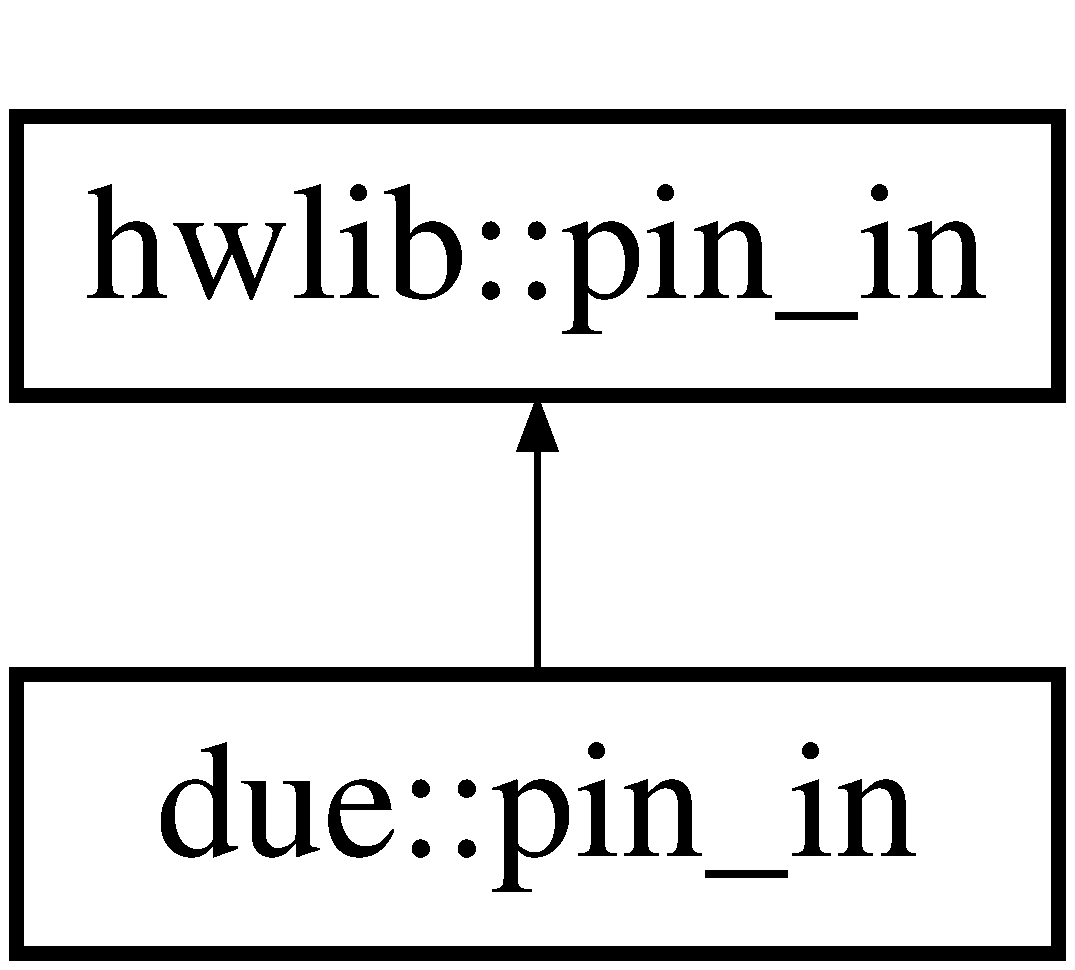
\includegraphics[height=2.000000cm]{classdue_1_1pin__in}
\end{center}
\end{figure}
\subsection*{Public Member Functions}
\begin{DoxyCompactItemize}
\item 
\hyperlink{classdue_1_1pin__in_ae57de72b79b4b603e46d518695742b3a}{pin\+\_\+in} (int port\+\_\+number, int pin\+\_\+number)
\begin{DoxyCompactList}\small\item\em Arduino Due \hyperlink{classdue_1_1pin__in}{pin\+\_\+in} constructor. \end{DoxyCompactList}\item 
\hyperlink{classdue_1_1pin__in_a91f66ca279e18ced46cf693bcf3c0935}{pin\+\_\+in} (\hyperlink{namespacedue_a8ffa3ec309934ff9db34317e504bcc92}{pins} name)
\begin{DoxyCompactList}\small\item\em Arduino Due \hyperlink{classdue_1_1pin__in}{pin\+\_\+in} constructor from a Due pin name. \end{DoxyCompactList}\item 
bool \hyperlink{classdue_1_1pin__in_abfadd4fd4c1aef21c1243bc69ce55b1c}{get} () override
\begin{DoxyCompactList}\small\item\em read the pin \end{DoxyCompactList}\end{DoxyCompactItemize}


\subsection{Detailed Description}
\hyperlink{classdue_1_1pin__in}{pin\+\_\+in} implementation for a A\+T\+S\+A\+M3\+X8E 

\subsection{Constructor \& Destructor Documentation}
\index{due\+::pin\+\_\+in@{due\+::pin\+\_\+in}!pin\+\_\+in@{pin\+\_\+in}}
\index{pin\+\_\+in@{pin\+\_\+in}!due\+::pin\+\_\+in@{due\+::pin\+\_\+in}}
\subsubsection[{\texorpdfstring{pin\+\_\+in(int port\+\_\+number, int pin\+\_\+number)}{pin_in(int port_number, int pin_number)}}]{\setlength{\rightskip}{0pt plus 5cm}due\+::pin\+\_\+in\+::pin\+\_\+in (
\begin{DoxyParamCaption}
\item[{int}]{port\+\_\+number, }
\item[{int}]{pin\+\_\+number}
\end{DoxyParamCaption}
)\hspace{0.3cm}{\ttfamily [inline]}}\hypertarget{classdue_1_1pin__in_ae57de72b79b4b603e46d518695742b3a}{}\label{classdue_1_1pin__in_ae57de72b79b4b603e46d518695742b3a}


Arduino Due \hyperlink{classdue_1_1pin__in}{pin\+\_\+in} constructor. 

Constructor for a A\+T\+S\+A\+M3\+X8E input pin.

The port\+\_\+number and pin\+\_\+number refer to the chip, not to the Arduino board pin names.

This constructor sets the pin direction to input. \index{due\+::pin\+\_\+in@{due\+::pin\+\_\+in}!pin\+\_\+in@{pin\+\_\+in}}
\index{pin\+\_\+in@{pin\+\_\+in}!due\+::pin\+\_\+in@{due\+::pin\+\_\+in}}
\subsubsection[{\texorpdfstring{pin\+\_\+in(pins name)}{pin_in(pins name)}}]{\setlength{\rightskip}{0pt plus 5cm}due\+::pin\+\_\+in\+::pin\+\_\+in (
\begin{DoxyParamCaption}
\item[{{\bf pins}}]{name}
\end{DoxyParamCaption}
)\hspace{0.3cm}{\ttfamily [inline]}}\hypertarget{classdue_1_1pin__in_a91f66ca279e18ced46cf693bcf3c0935}{}\label{classdue_1_1pin__in_a91f66ca279e18ced46cf693bcf3c0935}


Arduino Due \hyperlink{classdue_1_1pin__in}{pin\+\_\+in} constructor from a Due pin name. 

This call creates a \hyperlink{classdue_1_1pin__in}{pin\+\_\+in} from an Arduino Due pin name.

This constructor sets the pin direction to input. 

\subsection{Member Function Documentation}
\index{due\+::pin\+\_\+in@{due\+::pin\+\_\+in}!get@{get}}
\index{get@{get}!due\+::pin\+\_\+in@{due\+::pin\+\_\+in}}
\subsubsection[{\texorpdfstring{get() override}{get() override}}]{\setlength{\rightskip}{0pt plus 5cm}bool due\+::pin\+\_\+in\+::get (
\begin{DoxyParamCaption}
{}
\end{DoxyParamCaption}
)\hspace{0.3cm}{\ttfamily [inline]}, {\ttfamily [override]}, {\ttfamily [virtual]}}\hypertarget{classdue_1_1pin__in_abfadd4fd4c1aef21c1243bc69ce55b1c}{}\label{classdue_1_1pin__in_abfadd4fd4c1aef21c1243bc69ce55b1c}


read the pin 

This function returns the level of the pin. When the pin level is high the value true is returned, when the pin level is low the value false is returned. 

Implements \hyperlink{classhwlib_1_1pin__in_a5cbc123fa14d62c98dd41f7523cf6063}{hwlib\+::pin\+\_\+in}.



The documentation for this class was generated from the following file\+:\begin{DoxyCompactItemize}
\item 
\hyperlink{hwlib-due_8hpp}{hwlib-\/due.\+hpp}\end{DoxyCompactItemize}

\hypertarget{classhwlib_1_1pin__in}{}\section{hwlib\+:\+:pin\+\_\+in Class Reference}
\label{classhwlib_1_1pin__in}\index{hwlib\+::pin\+\_\+in@{hwlib\+::pin\+\_\+in}}


input pin interface  




{\ttfamily \#include $<$hwlib-\/pin.\+hpp$>$}

Inheritance diagram for hwlib\+:\+:pin\+\_\+in\+:\begin{figure}[H]
\begin{center}
\leavevmode
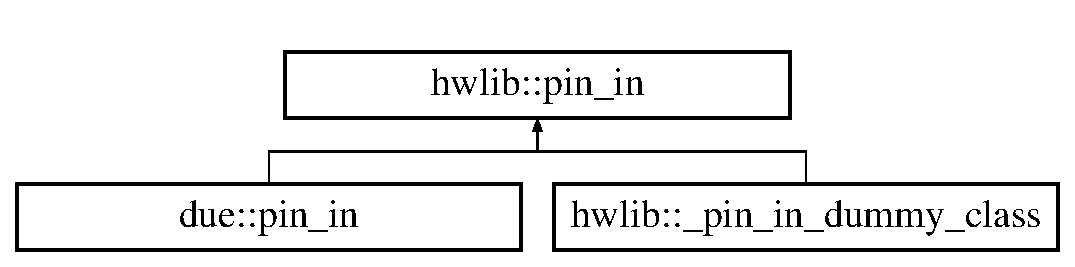
\includegraphics[height=2.000000cm]{classhwlib_1_1pin__in}
\end{center}
\end{figure}
\subsection*{Public Member Functions}
\begin{DoxyCompactItemize}
\item 
virtual bool \hyperlink{classhwlib_1_1pin__in_a5cbc123fa14d62c98dd41f7523cf6063}{get} ()=0
\begin{DoxyCompactList}\small\item\em read the pin \end{DoxyCompactList}\end{DoxyCompactItemize}


\subsection{Detailed Description}
input pin interface 

This class abstracts the interface for an input-\/only pin. 

\subsection{Member Function Documentation}
\index{hwlib\+::pin\+\_\+in@{hwlib\+::pin\+\_\+in}!get@{get}}
\index{get@{get}!hwlib\+::pin\+\_\+in@{hwlib\+::pin\+\_\+in}}
\subsubsection[{\texorpdfstring{get()=0}{get()=0}}]{\setlength{\rightskip}{0pt plus 5cm}virtual bool hwlib\+::pin\+\_\+in\+::get (
\begin{DoxyParamCaption}
{}
\end{DoxyParamCaption}
)\hspace{0.3cm}{\ttfamily [pure virtual]}}\hypertarget{classhwlib_1_1pin__in_a5cbc123fa14d62c98dd41f7523cf6063}{}\label{classhwlib_1_1pin__in_a5cbc123fa14d62c98dd41f7523cf6063}


read the pin 

This function returns the level of the pin. When the pin level is high the value true is returned, when the pin level is low the value false is returned. 

Implemented in \hyperlink{classdue_1_1pin__in_abfadd4fd4c1aef21c1243bc69ce55b1c}{due\+::pin\+\_\+in}, and \hyperlink{classhwlib_1_1__pin__in__dummy__class_a2b51c1a0d291cd4414e70504d388c9cb}{hwlib\+::\+\_\+pin\+\_\+in\+\_\+dummy\+\_\+class}.



The documentation for this class was generated from the following file\+:\begin{DoxyCompactItemize}
\item 
\hyperlink{hwlib-pin_8hpp}{hwlib-\/pin.\+hpp}\end{DoxyCompactItemize}

\hypertarget{classdue_1_1pin__in__out}{}\section{due\+:\+:pin\+\_\+in\+\_\+out Class Reference}
\label{classdue_1_1pin__in__out}\index{due\+::pin\+\_\+in\+\_\+out@{due\+::pin\+\_\+in\+\_\+out}}


\hyperlink{classdue_1_1pin__in__out}{pin\+\_\+in\+\_\+out} implementation for a A\+T\+S\+A\+M3\+X8E  




{\ttfamily \#include $<$hwlib-\/due.\+hpp$>$}

Inheritance diagram for due\+:\+:pin\+\_\+in\+\_\+out\+:\begin{figure}[H]
\begin{center}
\leavevmode
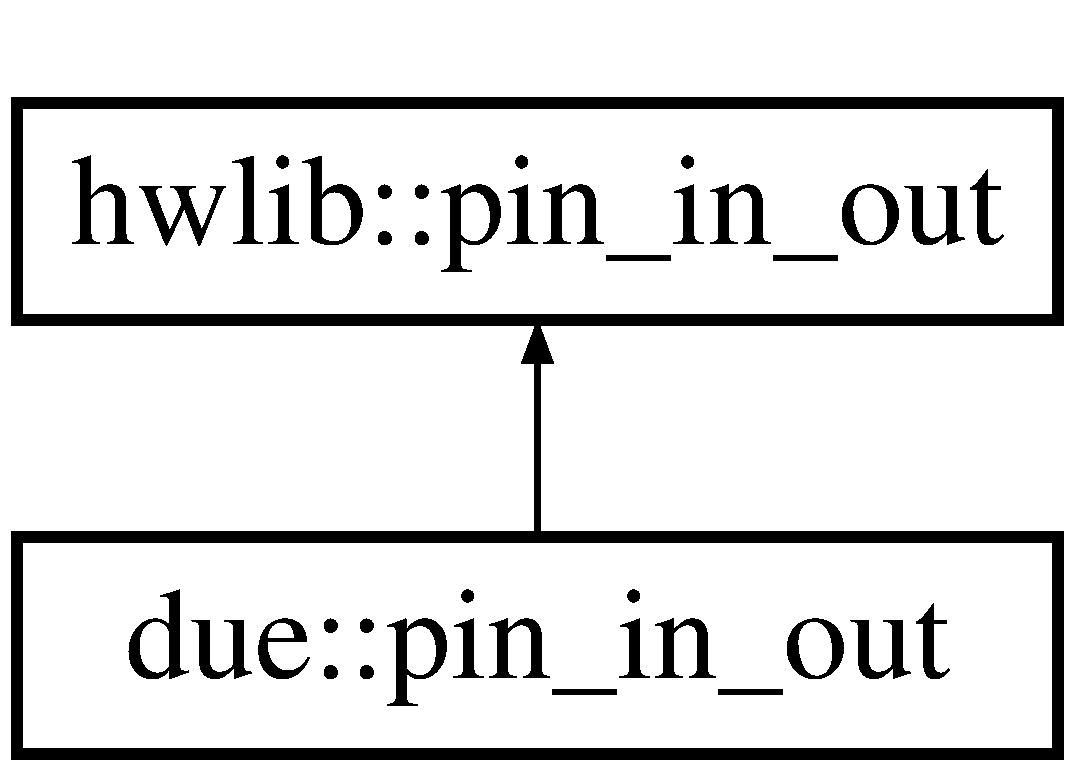
\includegraphics[height=2.000000cm]{classdue_1_1pin__in__out}
\end{center}
\end{figure}
\subsection*{Public Member Functions}
\begin{DoxyCompactItemize}
\item 
\hyperlink{classdue_1_1pin__in__out_a12f008036b3594228749c70f45cbdf9a}{pin\+\_\+in\+\_\+out} (int port\+\_\+number, int pin\+\_\+number)
\begin{DoxyCompactList}\small\item\em Arduino Due \hyperlink{classdue_1_1pin__out}{pin\+\_\+out} constructor. \end{DoxyCompactList}\item 
\hyperlink{classdue_1_1pin__in__out_a228da28eb609b180235db2a0ed249469}{pin\+\_\+in\+\_\+out} (\hyperlink{namespacedue_a8ffa3ec309934ff9db34317e504bcc92}{pins} name)
\begin{DoxyCompactList}\small\item\em Arduino Due \hyperlink{classdue_1_1pin__out}{pin\+\_\+out} constructor from a Due pin name. \end{DoxyCompactList}\item 
void \hyperlink{classdue_1_1pin__in__out_a2ca0c81a7e1059a171c997d5015d99ea}{direction\+\_\+set\+\_\+input} () override
\begin{DoxyCompactList}\small\item\em set the direction of a pin to input. \end{DoxyCompactList}\item 
bool \hyperlink{classdue_1_1pin__in__out_a09142f62d25f903475be52da0b3fe8a9}{get} () override
\begin{DoxyCompactList}\small\item\em read the pin \end{DoxyCompactList}\item 
void \hyperlink{classdue_1_1pin__in__out_a45f7cf2e7f71638337f82ecf1852f884}{direction\+\_\+set\+\_\+output} () override
\begin{DoxyCompactList}\small\item\em set the direction of a pin to output \end{DoxyCompactList}\item 
void \hyperlink{classdue_1_1pin__in__out_ad3a74cb13af59d4a5be3cc40a8f894b8}{set} (bool v) override
\begin{DoxyCompactList}\small\item\em write the pin \end{DoxyCompactList}\end{DoxyCompactItemize}


\subsection{Detailed Description}
\hyperlink{classdue_1_1pin__in__out}{pin\+\_\+in\+\_\+out} implementation for a A\+T\+S\+A\+M3\+X8E 

\subsection{Constructor \& Destructor Documentation}
\index{due\+::pin\+\_\+in\+\_\+out@{due\+::pin\+\_\+in\+\_\+out}!pin\+\_\+in\+\_\+out@{pin\+\_\+in\+\_\+out}}
\index{pin\+\_\+in\+\_\+out@{pin\+\_\+in\+\_\+out}!due\+::pin\+\_\+in\+\_\+out@{due\+::pin\+\_\+in\+\_\+out}}
\subsubsection[{\texorpdfstring{pin\+\_\+in\+\_\+out(int port\+\_\+number, int pin\+\_\+number)}{pin_in_out(int port_number, int pin_number)}}]{\setlength{\rightskip}{0pt plus 5cm}due\+::pin\+\_\+in\+\_\+out\+::pin\+\_\+in\+\_\+out (
\begin{DoxyParamCaption}
\item[{int}]{port\+\_\+number, }
\item[{int}]{pin\+\_\+number}
\end{DoxyParamCaption}
)\hspace{0.3cm}{\ttfamily [inline]}}\hypertarget{classdue_1_1pin__in__out_a12f008036b3594228749c70f45cbdf9a}{}\label{classdue_1_1pin__in__out_a12f008036b3594228749c70f45cbdf9a}


Arduino Due \hyperlink{classdue_1_1pin__out}{pin\+\_\+out} constructor. 

Constructor for a A\+T\+S\+A\+M3\+X8E input pin.

The port\+\_\+number and pin\+\_\+number refer to the chip, not to the Arduino board pin names.

This constructor doesn\textquotesingle{}t set the pin direction to input or output, a direction\+\_\+set function must be called to do so. \index{due\+::pin\+\_\+in\+\_\+out@{due\+::pin\+\_\+in\+\_\+out}!pin\+\_\+in\+\_\+out@{pin\+\_\+in\+\_\+out}}
\index{pin\+\_\+in\+\_\+out@{pin\+\_\+in\+\_\+out}!due\+::pin\+\_\+in\+\_\+out@{due\+::pin\+\_\+in\+\_\+out}}
\subsubsection[{\texorpdfstring{pin\+\_\+in\+\_\+out(pins name)}{pin_in_out(pins name)}}]{\setlength{\rightskip}{0pt plus 5cm}due\+::pin\+\_\+in\+\_\+out\+::pin\+\_\+in\+\_\+out (
\begin{DoxyParamCaption}
\item[{{\bf pins}}]{name}
\end{DoxyParamCaption}
)\hspace{0.3cm}{\ttfamily [inline]}}\hypertarget{classdue_1_1pin__in__out_a228da28eb609b180235db2a0ed249469}{}\label{classdue_1_1pin__in__out_a228da28eb609b180235db2a0ed249469}


Arduino Due \hyperlink{classdue_1_1pin__out}{pin\+\_\+out} constructor from a Due pin name. 

This call creates a \hyperlink{classdue_1_1pin__out}{pin\+\_\+out} from an Arduino Due pin name.

This constructor doesn\textquotesingle{}t set the pin direction to input or output, a direction\+\_\+set function must be called to do so. 

\subsection{Member Function Documentation}
\index{due\+::pin\+\_\+in\+\_\+out@{due\+::pin\+\_\+in\+\_\+out}!direction\+\_\+set\+\_\+input@{direction\+\_\+set\+\_\+input}}
\index{direction\+\_\+set\+\_\+input@{direction\+\_\+set\+\_\+input}!due\+::pin\+\_\+in\+\_\+out@{due\+::pin\+\_\+in\+\_\+out}}
\subsubsection[{\texorpdfstring{direction\+\_\+set\+\_\+input() override}{direction_set_input() override}}]{\setlength{\rightskip}{0pt plus 5cm}void due\+::pin\+\_\+in\+\_\+out\+::direction\+\_\+set\+\_\+input (
\begin{DoxyParamCaption}
{}
\end{DoxyParamCaption}
)\hspace{0.3cm}{\ttfamily [inline]}, {\ttfamily [override]}, {\ttfamily [virtual]}}\hypertarget{classdue_1_1pin__in__out_a2ca0c81a7e1059a171c997d5015d99ea}{}\label{classdue_1_1pin__in__out_a2ca0c81a7e1059a171c997d5015d99ea}


set the direction of a pin to input. 

Calling this function sets the pin identified by p to input. 

Implements \hyperlink{classhwlib_1_1pin__in__out_a54ce1a5086d3c9e7b868511b1d46acd0}{hwlib\+::pin\+\_\+in\+\_\+out}.

\index{due\+::pin\+\_\+in\+\_\+out@{due\+::pin\+\_\+in\+\_\+out}!direction\+\_\+set\+\_\+output@{direction\+\_\+set\+\_\+output}}
\index{direction\+\_\+set\+\_\+output@{direction\+\_\+set\+\_\+output}!due\+::pin\+\_\+in\+\_\+out@{due\+::pin\+\_\+in\+\_\+out}}
\subsubsection[{\texorpdfstring{direction\+\_\+set\+\_\+output() override}{direction_set_output() override}}]{\setlength{\rightskip}{0pt plus 5cm}void due\+::pin\+\_\+in\+\_\+out\+::direction\+\_\+set\+\_\+output (
\begin{DoxyParamCaption}
{}
\end{DoxyParamCaption}
)\hspace{0.3cm}{\ttfamily [inline]}, {\ttfamily [override]}, {\ttfamily [virtual]}}\hypertarget{classdue_1_1pin__in__out_a45f7cf2e7f71638337f82ecf1852f884}{}\label{classdue_1_1pin__in__out_a45f7cf2e7f71638337f82ecf1852f884}


set the direction of a pin to output 

Calling this function sets the pin identified by p to output. 

Implements \hyperlink{classhwlib_1_1pin__in__out_ad08a5f5e9a4c3aadaa7c665b98f2418e}{hwlib\+::pin\+\_\+in\+\_\+out}.

\index{due\+::pin\+\_\+in\+\_\+out@{due\+::pin\+\_\+in\+\_\+out}!get@{get}}
\index{get@{get}!due\+::pin\+\_\+in\+\_\+out@{due\+::pin\+\_\+in\+\_\+out}}
\subsubsection[{\texorpdfstring{get() override}{get() override}}]{\setlength{\rightskip}{0pt plus 5cm}bool due\+::pin\+\_\+in\+\_\+out\+::get (
\begin{DoxyParamCaption}
{}
\end{DoxyParamCaption}
)\hspace{0.3cm}{\ttfamily [inline]}, {\ttfamily [override]}, {\ttfamily [virtual]}}\hypertarget{classdue_1_1pin__in__out_a09142f62d25f903475be52da0b3fe8a9}{}\label{classdue_1_1pin__in__out_a09142f62d25f903475be52da0b3fe8a9}


read the pin 

This function returns the level of the pin. When the pin level is high the value true is returned, when the pin level is low the value false is returned.

Before calling this function the pin direction must have been set to input by calling \hyperlink{classdue_1_1pin__in__out_a2ca0c81a7e1059a171c997d5015d99ea}{direction\+\_\+set\+\_\+input()}. 

Implements \hyperlink{classhwlib_1_1pin__in__out_a298d32c19a8f94b730d34d4496bcf3ae}{hwlib\+::pin\+\_\+in\+\_\+out}.

\index{due\+::pin\+\_\+in\+\_\+out@{due\+::pin\+\_\+in\+\_\+out}!set@{set}}
\index{set@{set}!due\+::pin\+\_\+in\+\_\+out@{due\+::pin\+\_\+in\+\_\+out}}
\subsubsection[{\texorpdfstring{set(bool v) override}{set(bool v) override}}]{\setlength{\rightskip}{0pt plus 5cm}void due\+::pin\+\_\+in\+\_\+out\+::set (
\begin{DoxyParamCaption}
\item[{bool}]{x}
\end{DoxyParamCaption}
)\hspace{0.3cm}{\ttfamily [inline]}, {\ttfamily [override]}, {\ttfamily [virtual]}}\hypertarget{classdue_1_1pin__in__out_ad3a74cb13af59d4a5be3cc40a8f894b8}{}\label{classdue_1_1pin__in__out_ad3a74cb13af59d4a5be3cc40a8f894b8}


write the pin 

This function sets the level of the pin to the value v. A value of true makes the pin high, a value of false makes it low.

Before calling this function the pin direction must have been set to output by calling \hyperlink{classdue_1_1pin__in__out_a45f7cf2e7f71638337f82ecf1852f884}{direction\+\_\+set\+\_\+output()}. 

Implements \hyperlink{classhwlib_1_1pin__in__out_a198c4d27a9783f4c17e8f5dfd9aca6a9}{hwlib\+::pin\+\_\+in\+\_\+out}.



The documentation for this class was generated from the following file\+:\begin{DoxyCompactItemize}
\item 
\hyperlink{hwlib-due_8hpp}{hwlib-\/due.\+hpp}\end{DoxyCompactItemize}

\hypertarget{classhwlib_1_1pin__in__out}{}\section{hwlib\+:\+:pin\+\_\+in\+\_\+out Class Reference}
\label{classhwlib_1_1pin__in__out}\index{hwlib\+::pin\+\_\+in\+\_\+out@{hwlib\+::pin\+\_\+in\+\_\+out}}


input/output pin interface  




{\ttfamily \#include $<$hwlib-\/pin.\+hpp$>$}

Inheritance diagram for hwlib\+:\+:pin\+\_\+in\+\_\+out\+:\begin{figure}[H]
\begin{center}
\leavevmode
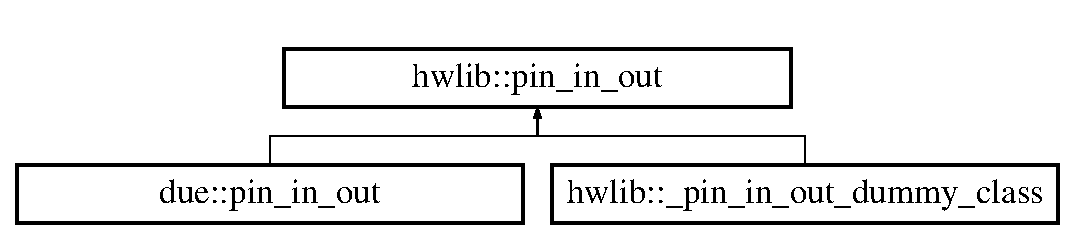
\includegraphics[height=2.000000cm]{classhwlib_1_1pin__in__out}
\end{center}
\end{figure}
\subsection*{Public Member Functions}
\begin{DoxyCompactItemize}
\item 
virtual void \hyperlink{classhwlib_1_1pin__in__out_a54ce1a5086d3c9e7b868511b1d46acd0}{direction\+\_\+set\+\_\+input} ()=0
\begin{DoxyCompactList}\small\item\em set the direction of a pin to input. \end{DoxyCompactList}\item 
virtual bool \hyperlink{classhwlib_1_1pin__in__out_a298d32c19a8f94b730d34d4496bcf3ae}{get} ()=0
\begin{DoxyCompactList}\small\item\em read the pin \end{DoxyCompactList}\item 
virtual void \hyperlink{classhwlib_1_1pin__in__out_ad08a5f5e9a4c3aadaa7c665b98f2418e}{direction\+\_\+set\+\_\+output} ()=0
\begin{DoxyCompactList}\small\item\em set the direction of a pin to output \end{DoxyCompactList}\item 
virtual void \hyperlink{classhwlib_1_1pin__in__out_a198c4d27a9783f4c17e8f5dfd9aca6a9}{set} (bool x)=0
\begin{DoxyCompactList}\small\item\em write the pin \end{DoxyCompactList}\end{DoxyCompactItemize}


\subsection{Detailed Description}
input/output pin interface 

This class abstracts the interface for an input/output pin. 

\subsection{Member Function Documentation}
\index{hwlib\+::pin\+\_\+in\+\_\+out@{hwlib\+::pin\+\_\+in\+\_\+out}!direction\+\_\+set\+\_\+input@{direction\+\_\+set\+\_\+input}}
\index{direction\+\_\+set\+\_\+input@{direction\+\_\+set\+\_\+input}!hwlib\+::pin\+\_\+in\+\_\+out@{hwlib\+::pin\+\_\+in\+\_\+out}}
\subsubsection[{\texorpdfstring{direction\+\_\+set\+\_\+input()=0}{direction_set_input()=0}}]{\setlength{\rightskip}{0pt plus 5cm}virtual void hwlib\+::pin\+\_\+in\+\_\+out\+::direction\+\_\+set\+\_\+input (
\begin{DoxyParamCaption}
{}
\end{DoxyParamCaption}
)\hspace{0.3cm}{\ttfamily [pure virtual]}}\hypertarget{classhwlib_1_1pin__in__out_a54ce1a5086d3c9e7b868511b1d46acd0}{}\label{classhwlib_1_1pin__in__out_a54ce1a5086d3c9e7b868511b1d46acd0}


set the direction of a pin to input. 

Calling this function sets the pin identified by p to input. 

Implemented in \hyperlink{classdue_1_1pin__in__out_a2ca0c81a7e1059a171c997d5015d99ea}{due\+::pin\+\_\+in\+\_\+out}, and \hyperlink{classhwlib_1_1__pin__in__out__dummy__class_a29f385015d361cfa434a625ca8331cd7}{hwlib\+::\+\_\+pin\+\_\+in\+\_\+out\+\_\+dummy\+\_\+class}.

\index{hwlib\+::pin\+\_\+in\+\_\+out@{hwlib\+::pin\+\_\+in\+\_\+out}!direction\+\_\+set\+\_\+output@{direction\+\_\+set\+\_\+output}}
\index{direction\+\_\+set\+\_\+output@{direction\+\_\+set\+\_\+output}!hwlib\+::pin\+\_\+in\+\_\+out@{hwlib\+::pin\+\_\+in\+\_\+out}}
\subsubsection[{\texorpdfstring{direction\+\_\+set\+\_\+output()=0}{direction_set_output()=0}}]{\setlength{\rightskip}{0pt plus 5cm}virtual void hwlib\+::pin\+\_\+in\+\_\+out\+::direction\+\_\+set\+\_\+output (
\begin{DoxyParamCaption}
{}
\end{DoxyParamCaption}
)\hspace{0.3cm}{\ttfamily [pure virtual]}}\hypertarget{classhwlib_1_1pin__in__out_ad08a5f5e9a4c3aadaa7c665b98f2418e}{}\label{classhwlib_1_1pin__in__out_ad08a5f5e9a4c3aadaa7c665b98f2418e}


set the direction of a pin to output 

Calling this function sets the pin identified by p to output. 

Implemented in \hyperlink{classdue_1_1pin__in__out_a45f7cf2e7f71638337f82ecf1852f884}{due\+::pin\+\_\+in\+\_\+out}, and \hyperlink{classhwlib_1_1__pin__in__out__dummy__class_a551f4d543e9fccd85ad843cbd9258a94}{hwlib\+::\+\_\+pin\+\_\+in\+\_\+out\+\_\+dummy\+\_\+class}.

\index{hwlib\+::pin\+\_\+in\+\_\+out@{hwlib\+::pin\+\_\+in\+\_\+out}!get@{get}}
\index{get@{get}!hwlib\+::pin\+\_\+in\+\_\+out@{hwlib\+::pin\+\_\+in\+\_\+out}}
\subsubsection[{\texorpdfstring{get()=0}{get()=0}}]{\setlength{\rightskip}{0pt plus 5cm}virtual bool hwlib\+::pin\+\_\+in\+\_\+out\+::get (
\begin{DoxyParamCaption}
{}
\end{DoxyParamCaption}
)\hspace{0.3cm}{\ttfamily [pure virtual]}}\hypertarget{classhwlib_1_1pin__in__out_a298d32c19a8f94b730d34d4496bcf3ae}{}\label{classhwlib_1_1pin__in__out_a298d32c19a8f94b730d34d4496bcf3ae}


read the pin 

This function returns the level of the pin. When the pin level is high the value true is returned, when the pin level is low the value false is returned.

Before calling this function the pin direction must have been set to input by calling \hyperlink{classhwlib_1_1pin__in__out_a54ce1a5086d3c9e7b868511b1d46acd0}{direction\+\_\+set\+\_\+input()}. 

Implemented in \hyperlink{classdue_1_1pin__in__out_a09142f62d25f903475be52da0b3fe8a9}{due\+::pin\+\_\+in\+\_\+out}, and \hyperlink{classhwlib_1_1__pin__in__out__dummy__class_aa3a8d3f46143f6bb042444dee00c34c6}{hwlib\+::\+\_\+pin\+\_\+in\+\_\+out\+\_\+dummy\+\_\+class}.

\index{hwlib\+::pin\+\_\+in\+\_\+out@{hwlib\+::pin\+\_\+in\+\_\+out}!set@{set}}
\index{set@{set}!hwlib\+::pin\+\_\+in\+\_\+out@{hwlib\+::pin\+\_\+in\+\_\+out}}
\subsubsection[{\texorpdfstring{set(bool x)=0}{set(bool x)=0}}]{\setlength{\rightskip}{0pt plus 5cm}virtual void hwlib\+::pin\+\_\+in\+\_\+out\+::set (
\begin{DoxyParamCaption}
\item[{bool}]{x}
\end{DoxyParamCaption}
)\hspace{0.3cm}{\ttfamily [pure virtual]}}\hypertarget{classhwlib_1_1pin__in__out_a198c4d27a9783f4c17e8f5dfd9aca6a9}{}\label{classhwlib_1_1pin__in__out_a198c4d27a9783f4c17e8f5dfd9aca6a9}


write the pin 

This function sets the level of the pin to the value v. A value of true makes the pin high, a value of false makes it low.

Before calling this function the pin direction must have been set to output by calling \hyperlink{classhwlib_1_1pin__in__out_ad08a5f5e9a4c3aadaa7c665b98f2418e}{direction\+\_\+set\+\_\+output()}. 

Implemented in \hyperlink{classdue_1_1pin__in__out_ad3a74cb13af59d4a5be3cc40a8f894b8}{due\+::pin\+\_\+in\+\_\+out}, and \hyperlink{classhwlib_1_1__pin__in__out__dummy__class_afd92206adb4c05526a84d8e7ff17491c}{hwlib\+::\+\_\+pin\+\_\+in\+\_\+out\+\_\+dummy\+\_\+class}.



The documentation for this class was generated from the following file\+:\begin{DoxyCompactItemize}
\item 
\hyperlink{hwlib-pin_8hpp}{hwlib-\/pin.\+hpp}\end{DoxyCompactItemize}

\hypertarget{classdue_1_1pin__oc}{}\section{due\+:\+:pin\+\_\+oc Class Reference}
\label{classdue_1_1pin__oc}\index{due\+::pin\+\_\+oc@{due\+::pin\+\_\+oc}}


\hyperlink{classdue_1_1pin__oc}{pin\+\_\+oc} implementation for a A\+T\+S\+A\+M3\+X8E  




{\ttfamily \#include $<$hwlib-\/due.\+hpp$>$}

Inheritance diagram for due\+:\+:pin\+\_\+oc\+:\begin{figure}[H]
\begin{center}
\leavevmode
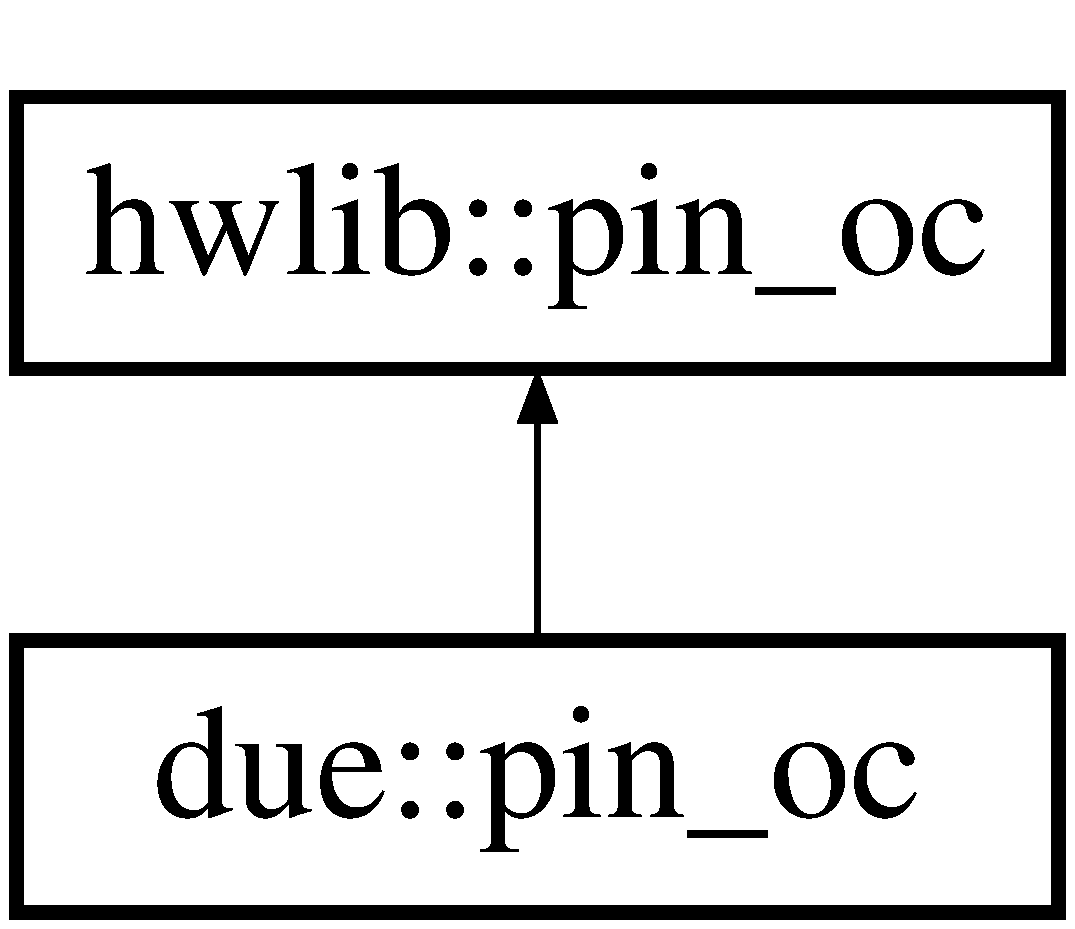
\includegraphics[height=2.000000cm]{classdue_1_1pin__oc}
\end{center}
\end{figure}
\subsection*{Public Member Functions}
\begin{DoxyCompactItemize}
\item 
\hyperlink{classdue_1_1pin__oc_a104511f36b1b493b8164fc91e2a160c3}{pin\+\_\+oc} (int port\+\_\+number, int pin\+\_\+number)
\begin{DoxyCompactList}\small\item\em Arduino Due \hyperlink{classdue_1_1pin__oc}{pin\+\_\+oc} constructor. \end{DoxyCompactList}\item 
\hyperlink{classdue_1_1pin__oc_a26daecda4236219f16e896cb82e9e6aa}{pin\+\_\+oc} (\hyperlink{namespacedue_a8ffa3ec309934ff9db34317e504bcc92}{pins} name)
\begin{DoxyCompactList}\small\item\em Arduino Due \hyperlink{classdue_1_1pin__oc}{pin\+\_\+oc} constructor from a Due pin name. \end{DoxyCompactList}\item 
bool \hyperlink{classdue_1_1pin__oc_a7d90e525b3531e099e5ced6f531dff81}{get} () override
\begin{DoxyCompactList}\small\item\em read the pin \end{DoxyCompactList}\item 
void \hyperlink{classdue_1_1pin__oc_acfeab83375e9620804e87d695d3ea3b4}{set} (bool v) override
\begin{DoxyCompactList}\small\item\em write the pin \end{DoxyCompactList}\end{DoxyCompactItemize}


\subsection{Detailed Description}
\hyperlink{classdue_1_1pin__oc}{pin\+\_\+oc} implementation for a A\+T\+S\+A\+M3\+X8E 

\subsection{Constructor \& Destructor Documentation}
\index{due\+::pin\+\_\+oc@{due\+::pin\+\_\+oc}!pin\+\_\+oc@{pin\+\_\+oc}}
\index{pin\+\_\+oc@{pin\+\_\+oc}!due\+::pin\+\_\+oc@{due\+::pin\+\_\+oc}}
\subsubsection[{\texorpdfstring{pin\+\_\+oc(int port\+\_\+number, int pin\+\_\+number)}{pin_oc(int port_number, int pin_number)}}]{\setlength{\rightskip}{0pt plus 5cm}due\+::pin\+\_\+oc\+::pin\+\_\+oc (
\begin{DoxyParamCaption}
\item[{int}]{port\+\_\+number, }
\item[{int}]{pin\+\_\+number}
\end{DoxyParamCaption}
)\hspace{0.3cm}{\ttfamily [inline]}}\hypertarget{classdue_1_1pin__oc_a104511f36b1b493b8164fc91e2a160c3}{}\label{classdue_1_1pin__oc_a104511f36b1b493b8164fc91e2a160c3}


Arduino Due \hyperlink{classdue_1_1pin__oc}{pin\+\_\+oc} constructor. 

Constructor for a A\+T\+S\+A\+M3\+X8E input pin.

The port\+\_\+number and pin\+\_\+number refer to the chip, not to the Arduino board pin names.

This constructor sets the pin to high (high-\/impedance). \index{due\+::pin\+\_\+oc@{due\+::pin\+\_\+oc}!pin\+\_\+oc@{pin\+\_\+oc}}
\index{pin\+\_\+oc@{pin\+\_\+oc}!due\+::pin\+\_\+oc@{due\+::pin\+\_\+oc}}
\subsubsection[{\texorpdfstring{pin\+\_\+oc(pins name)}{pin_oc(pins name)}}]{\setlength{\rightskip}{0pt plus 5cm}due\+::pin\+\_\+oc\+::pin\+\_\+oc (
\begin{DoxyParamCaption}
\item[{{\bf pins}}]{name}
\end{DoxyParamCaption}
)\hspace{0.3cm}{\ttfamily [inline]}}\hypertarget{classdue_1_1pin__oc_a26daecda4236219f16e896cb82e9e6aa}{}\label{classdue_1_1pin__oc_a26daecda4236219f16e896cb82e9e6aa}


Arduino Due \hyperlink{classdue_1_1pin__oc}{pin\+\_\+oc} constructor from a Due pin name. 

This call creates a \hyperlink{classdue_1_1pin__oc}{pin\+\_\+oc} from an Arduino Due pin name.

This constructor sets the pin to high (high-\/impedance). 

\subsection{Member Function Documentation}
\index{due\+::pin\+\_\+oc@{due\+::pin\+\_\+oc}!get@{get}}
\index{get@{get}!due\+::pin\+\_\+oc@{due\+::pin\+\_\+oc}}
\subsubsection[{\texorpdfstring{get() override}{get() override}}]{\setlength{\rightskip}{0pt plus 5cm}bool due\+::pin\+\_\+oc\+::get (
\begin{DoxyParamCaption}
{}
\end{DoxyParamCaption}
)\hspace{0.3cm}{\ttfamily [inline]}, {\ttfamily [override]}, {\ttfamily [virtual]}}\hypertarget{classdue_1_1pin__oc_a7d90e525b3531e099e5ced6f531dff81}{}\label{classdue_1_1pin__oc_a7d90e525b3531e099e5ced6f531dff81}


read the pin 

This function returns the level of the pin. When the pin level is high the value true is returned, when the pin level is low the value false is returned.

This function can be called after set( false ) has been called on the pin, but then the level will read low (false). Call set( true ) to let the line float (presumably pulled high by a pull-\/up resistor) to read the level put on the line by an external device. 

Implements \hyperlink{classhwlib_1_1pin__oc_aa395bf9608ca48ca07dee2f5dc4612bd}{hwlib\+::pin\+\_\+oc}.

\index{due\+::pin\+\_\+oc@{due\+::pin\+\_\+oc}!set@{set}}
\index{set@{set}!due\+::pin\+\_\+oc@{due\+::pin\+\_\+oc}}
\subsubsection[{\texorpdfstring{set(bool v) override}{set(bool v) override}}]{\setlength{\rightskip}{0pt plus 5cm}void due\+::pin\+\_\+oc\+::set (
\begin{DoxyParamCaption}
\item[{bool}]{x}
\end{DoxyParamCaption}
)\hspace{0.3cm}{\ttfamily [inline]}, {\ttfamily [override]}, {\ttfamily [virtual]}}\hypertarget{classdue_1_1pin__oc_acfeab83375e9620804e87d695d3ea3b4}{}\label{classdue_1_1pin__oc_acfeab83375e9620804e87d695d3ea3b4}


write the pin 

This function sets the level of the pin to the value v. A value of true makes the pin hihg-\/impedance (presumably pulled high by a pull-\/up resistor), a value of false makes it low. 

Implements \hyperlink{classhwlib_1_1pin__oc_a2165622dad253a423d2fa52cbed7c553}{hwlib\+::pin\+\_\+oc}.



The documentation for this class was generated from the following file\+:\begin{DoxyCompactItemize}
\item 
\hyperlink{hwlib-due_8hpp}{hwlib-\/due.\+hpp}\end{DoxyCompactItemize}

\hypertarget{classhwlib_1_1pin__oc}{}\section{hwlib\+:\+:pin\+\_\+oc Class Reference}
\label{classhwlib_1_1pin__oc}\index{hwlib\+::pin\+\_\+oc@{hwlib\+::pin\+\_\+oc}}


open-\/collector input/output pin interface  




{\ttfamily \#include $<$hwlib-\/pin.\+hpp$>$}

Inheritance diagram for hwlib\+:\+:pin\+\_\+oc\+:\begin{figure}[H]
\begin{center}
\leavevmode
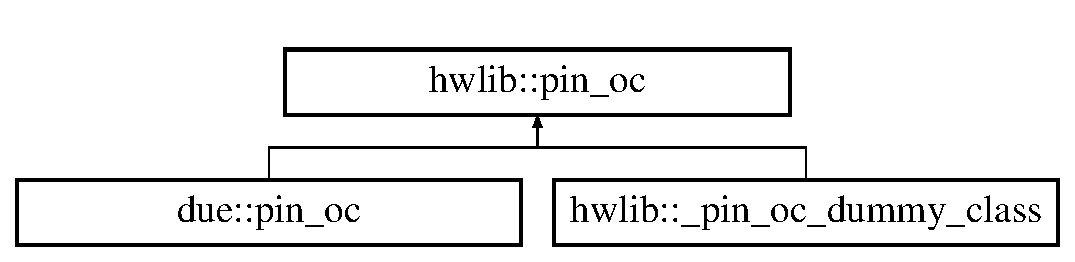
\includegraphics[height=2.000000cm]{classhwlib_1_1pin__oc}
\end{center}
\end{figure}
\subsection*{Public Member Functions}
\begin{DoxyCompactItemize}
\item 
virtual bool \hyperlink{classhwlib_1_1pin__oc_aa395bf9608ca48ca07dee2f5dc4612bd}{get} ()=0
\begin{DoxyCompactList}\small\item\em read the pin \end{DoxyCompactList}\item 
virtual void \hyperlink{classhwlib_1_1pin__oc_a2165622dad253a423d2fa52cbed7c553}{set} (bool x)=0
\begin{DoxyCompactList}\small\item\em write the pin \end{DoxyCompactList}\end{DoxyCompactItemize}


\subsection{Detailed Description}
open-\/collector input/output pin interface 

This class abstracts the interface for an open-\/collector input/output pin. 

\subsection{Member Function Documentation}
\index{hwlib\+::pin\+\_\+oc@{hwlib\+::pin\+\_\+oc}!get@{get}}
\index{get@{get}!hwlib\+::pin\+\_\+oc@{hwlib\+::pin\+\_\+oc}}
\subsubsection[{\texorpdfstring{get()=0}{get()=0}}]{\setlength{\rightskip}{0pt plus 5cm}virtual bool hwlib\+::pin\+\_\+oc\+::get (
\begin{DoxyParamCaption}
{}
\end{DoxyParamCaption}
)\hspace{0.3cm}{\ttfamily [pure virtual]}}\hypertarget{classhwlib_1_1pin__oc_aa395bf9608ca48ca07dee2f5dc4612bd}{}\label{classhwlib_1_1pin__oc_aa395bf9608ca48ca07dee2f5dc4612bd}


read the pin 

This function returns the level of the pin. When the pin level is high the value true is returned, when the pin level is low the value false is returned.

This function can be called after set( false ) has been called on the pin, but then the level will read low (false). Call set( true ) to let the line float (presumably pulled high by a pull-\/up resistor) to read the level put on the line by an external device. 

Implemented in \hyperlink{classdue_1_1pin__oc_a7d90e525b3531e099e5ced6f531dff81}{due\+::pin\+\_\+oc}, and \hyperlink{classhwlib_1_1__pin__oc__dummy__class_a06d061b7dd08d290e56969e90d4ff255}{hwlib\+::\+\_\+pin\+\_\+oc\+\_\+dummy\+\_\+class}.

\index{hwlib\+::pin\+\_\+oc@{hwlib\+::pin\+\_\+oc}!set@{set}}
\index{set@{set}!hwlib\+::pin\+\_\+oc@{hwlib\+::pin\+\_\+oc}}
\subsubsection[{\texorpdfstring{set(bool x)=0}{set(bool x)=0}}]{\setlength{\rightskip}{0pt plus 5cm}virtual void hwlib\+::pin\+\_\+oc\+::set (
\begin{DoxyParamCaption}
\item[{bool}]{x}
\end{DoxyParamCaption}
)\hspace{0.3cm}{\ttfamily [pure virtual]}}\hypertarget{classhwlib_1_1pin__oc_a2165622dad253a423d2fa52cbed7c553}{}\label{classhwlib_1_1pin__oc_a2165622dad253a423d2fa52cbed7c553}


write the pin 

This function sets the level of the pin to the value v. A value of true makes the pin hihg-\/impedance (presumably pulled high by a pull-\/up resistor), a value of false makes it low. 

Implemented in \hyperlink{classdue_1_1pin__oc_acfeab83375e9620804e87d695d3ea3b4}{due\+::pin\+\_\+oc}, and \hyperlink{classhwlib_1_1__pin__oc__dummy__class_a10db7f81b4ed0dc0573f039d97c1d69e}{hwlib\+::\+\_\+pin\+\_\+oc\+\_\+dummy\+\_\+class}.



The documentation for this class was generated from the following file\+:\begin{DoxyCompactItemize}
\item 
\hyperlink{hwlib-pin_8hpp}{hwlib-\/pin.\+hpp}\end{DoxyCompactItemize}

\hypertarget{classhwlib_1_1pin__out}{}\section{hwlib\+:\+:pin\+\_\+out Class Reference}
\label{classhwlib_1_1pin__out}\index{hwlib\+::pin\+\_\+out@{hwlib\+::pin\+\_\+out}}


output pin interface  




{\ttfamily \#include $<$hwlib-\/pin.\+hpp$>$}

Inheritance diagram for hwlib\+:\+:pin\+\_\+out\+:\begin{figure}[H]
\begin{center}
\leavevmode
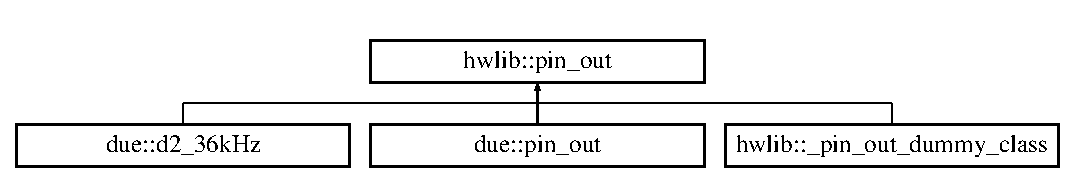
\includegraphics[height=2.000000cm]{classhwlib_1_1pin__out}
\end{center}
\end{figure}
\subsection*{Public Member Functions}
\begin{DoxyCompactItemize}
\item 
virtual void \hyperlink{classhwlib_1_1pin__out_af5c3a533f1a00ba973e37e60fb8c08c6}{set} (bool v)=0
\begin{DoxyCompactList}\small\item\em write the pin \end{DoxyCompactList}\end{DoxyCompactItemize}


\subsection{Detailed Description}
output pin interface 

This class abstracts the interface for an output-\/only pin. 

\subsection{Member Function Documentation}
\index{hwlib\+::pin\+\_\+out@{hwlib\+::pin\+\_\+out}!set@{set}}
\index{set@{set}!hwlib\+::pin\+\_\+out@{hwlib\+::pin\+\_\+out}}
\subsubsection[{\texorpdfstring{set(bool v)=0}{set(bool v)=0}}]{\setlength{\rightskip}{0pt plus 5cm}virtual void hwlib\+::pin\+\_\+out\+::set (
\begin{DoxyParamCaption}
\item[{bool}]{v}
\end{DoxyParamCaption}
)\hspace{0.3cm}{\ttfamily [pure virtual]}}\hypertarget{classhwlib_1_1pin__out_af5c3a533f1a00ba973e37e60fb8c08c6}{}\label{classhwlib_1_1pin__out_af5c3a533f1a00ba973e37e60fb8c08c6}


write the pin 

This function sets the level of the pin to the value v. A value of true makes the pin high, a value of false makes it low. 

Implemented in \hyperlink{classdue_1_1d2__36k_hz_abdb0b8ee44017ecfaf37fcbf9e0ba126}{due\+::d2\+\_\+36k\+Hz}, \hyperlink{classdue_1_1pin__out_a65a516d8139c1efb217d90f5bdffe0a4}{due\+::pin\+\_\+out}, and \hyperlink{classhwlib_1_1__pin__out__dummy__class_a2a1c7ef6046fbf45a92f5036632e4655}{hwlib\+::\+\_\+pin\+\_\+out\+\_\+dummy\+\_\+class}.



The documentation for this class was generated from the following file\+:\begin{DoxyCompactItemize}
\item 
\hyperlink{hwlib-pin_8hpp}{hwlib-\/pin.\+hpp}\end{DoxyCompactItemize}

\hypertarget{classdue_1_1pin__out}{}\section{due\+:\+:pin\+\_\+out Class Reference}
\label{classdue_1_1pin__out}\index{due\+::pin\+\_\+out@{due\+::pin\+\_\+out}}


\hyperlink{classdue_1_1pin__out}{pin\+\_\+out} implementation for a A\+T\+S\+A\+M3\+X8E  




{\ttfamily \#include $<$hwlib-\/due.\+hpp$>$}

Inheritance diagram for due\+:\+:pin\+\_\+out\+:\begin{figure}[H]
\begin{center}
\leavevmode
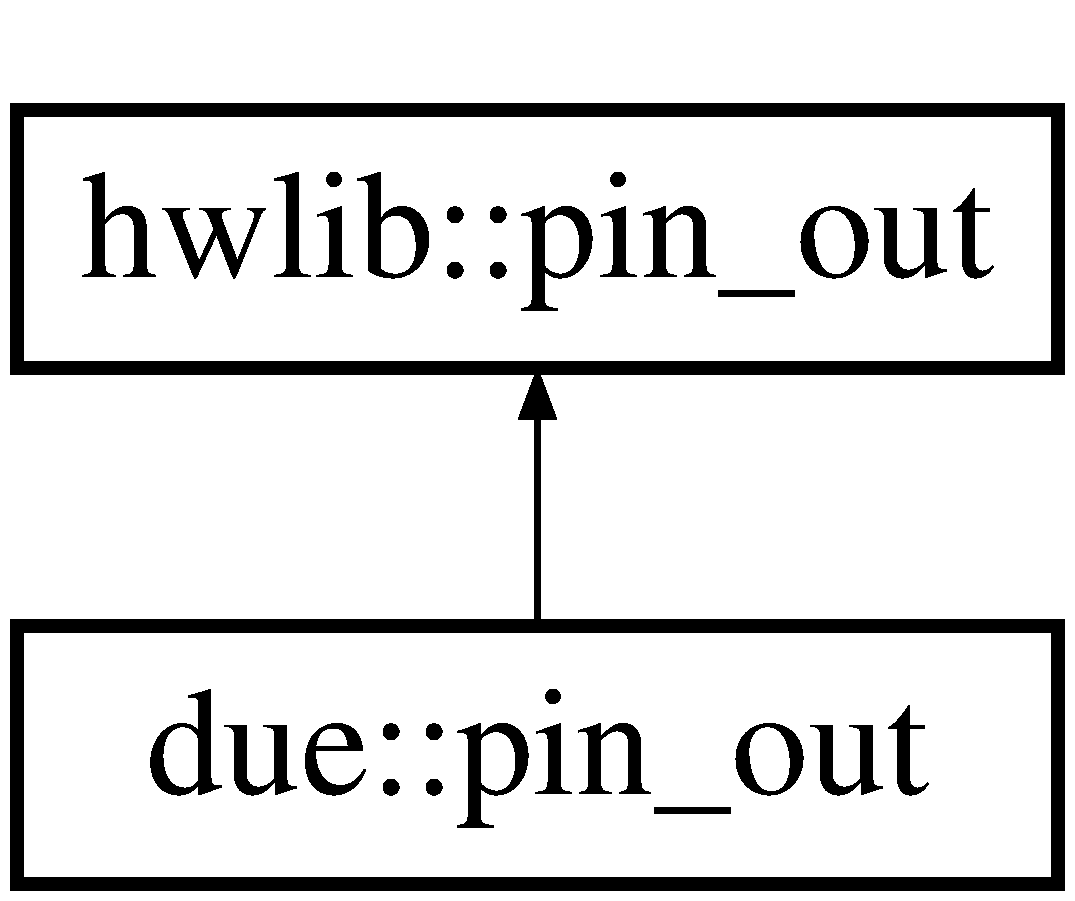
\includegraphics[height=2.000000cm]{classdue_1_1pin__out}
\end{center}
\end{figure}
\subsection*{Public Member Functions}
\begin{DoxyCompactItemize}
\item 
\hyperlink{classdue_1_1pin__out_aed112fcb4fa183b5114eeb90385b03f3}{pin\+\_\+out} (int port\+\_\+number, int pin\+\_\+number)
\begin{DoxyCompactList}\small\item\em Arduino Due \hyperlink{classdue_1_1pin__out}{pin\+\_\+out} constructor. \end{DoxyCompactList}\item 
\hyperlink{classdue_1_1pin__out_ad0ede1c3e5e7501ae0dd045d83578c6c}{pin\+\_\+out} (\hyperlink{namespacedue_a8ffa3ec309934ff9db34317e504bcc92}{pins} name)
\begin{DoxyCompactList}\small\item\em Arduino Due \hyperlink{classdue_1_1pin__out}{pin\+\_\+out} constructor from a Due pin name. \end{DoxyCompactList}\item 
void \hyperlink{classdue_1_1pin__out_a65a516d8139c1efb217d90f5bdffe0a4}{set} (bool v) override
\begin{DoxyCompactList}\small\item\em write the pin \end{DoxyCompactList}\end{DoxyCompactItemize}


\subsection{Detailed Description}
\hyperlink{classdue_1_1pin__out}{pin\+\_\+out} implementation for a A\+T\+S\+A\+M3\+X8E 

\subsection{Constructor \& Destructor Documentation}
\index{due\+::pin\+\_\+out@{due\+::pin\+\_\+out}!pin\+\_\+out@{pin\+\_\+out}}
\index{pin\+\_\+out@{pin\+\_\+out}!due\+::pin\+\_\+out@{due\+::pin\+\_\+out}}
\subsubsection[{\texorpdfstring{pin\+\_\+out(int port\+\_\+number, int pin\+\_\+number)}{pin_out(int port_number, int pin_number)}}]{\setlength{\rightskip}{0pt plus 5cm}due\+::pin\+\_\+out\+::pin\+\_\+out (
\begin{DoxyParamCaption}
\item[{int}]{port\+\_\+number, }
\item[{int}]{pin\+\_\+number}
\end{DoxyParamCaption}
)\hspace{0.3cm}{\ttfamily [inline]}}\hypertarget{classdue_1_1pin__out_aed112fcb4fa183b5114eeb90385b03f3}{}\label{classdue_1_1pin__out_aed112fcb4fa183b5114eeb90385b03f3}


Arduino Due \hyperlink{classdue_1_1pin__out}{pin\+\_\+out} constructor. 

Constructor for a A\+T\+S\+A\+M3\+X8E input pin.

The port\+\_\+number and pin\+\_\+number refer to the chip, not to the Arduino board pin names.

This constructor sets the pin direction to output. \index{due\+::pin\+\_\+out@{due\+::pin\+\_\+out}!pin\+\_\+out@{pin\+\_\+out}}
\index{pin\+\_\+out@{pin\+\_\+out}!due\+::pin\+\_\+out@{due\+::pin\+\_\+out}}
\subsubsection[{\texorpdfstring{pin\+\_\+out(pins name)}{pin_out(pins name)}}]{\setlength{\rightskip}{0pt plus 5cm}due\+::pin\+\_\+out\+::pin\+\_\+out (
\begin{DoxyParamCaption}
\item[{{\bf pins}}]{name}
\end{DoxyParamCaption}
)\hspace{0.3cm}{\ttfamily [inline]}}\hypertarget{classdue_1_1pin__out_ad0ede1c3e5e7501ae0dd045d83578c6c}{}\label{classdue_1_1pin__out_ad0ede1c3e5e7501ae0dd045d83578c6c}


Arduino Due \hyperlink{classdue_1_1pin__out}{pin\+\_\+out} constructor from a Due pin name. 

This call creates a \hyperlink{classdue_1_1pin__out}{pin\+\_\+out} from an Arduino Due pin name.

This constructor sets the pin direction to output. 

\subsection{Member Function Documentation}
\index{due\+::pin\+\_\+out@{due\+::pin\+\_\+out}!set@{set}}
\index{set@{set}!due\+::pin\+\_\+out@{due\+::pin\+\_\+out}}
\subsubsection[{\texorpdfstring{set(bool v) override}{set(bool v) override}}]{\setlength{\rightskip}{0pt plus 5cm}void due\+::pin\+\_\+out\+::set (
\begin{DoxyParamCaption}
\item[{bool}]{v}
\end{DoxyParamCaption}
)\hspace{0.3cm}{\ttfamily [inline]}, {\ttfamily [override]}, {\ttfamily [virtual]}}\hypertarget{classdue_1_1pin__out_a65a516d8139c1efb217d90f5bdffe0a4}{}\label{classdue_1_1pin__out_a65a516d8139c1efb217d90f5bdffe0a4}


write the pin 

This function sets the level of the pin to the value v. A value of true makes the pin high, a value of false makes it low. 

Implements \hyperlink{classhwlib_1_1pin__out_af5c3a533f1a00ba973e37e60fb8c08c6}{hwlib\+::pin\+\_\+out}.



The documentation for this class was generated from the following file\+:\begin{DoxyCompactItemize}
\item 
\hyperlink{hwlib-due_8hpp}{hwlib-\/due.\+hpp}\end{DoxyCompactItemize}

\hypertarget{classhwlib_1_1port__in}{}\section{hwlib\+:\+:port\+\_\+in Class Reference}
\label{classhwlib_1_1port__in}\index{hwlib\+::port\+\_\+in@{hwlib\+::port\+\_\+in}}


input port interface  




{\ttfamily \#include $<$hwlib-\/port.\+hpp$>$}

Inheritance diagram for hwlib\+:\+:port\+\_\+in\+:\begin{figure}[H]
\begin{center}
\leavevmode
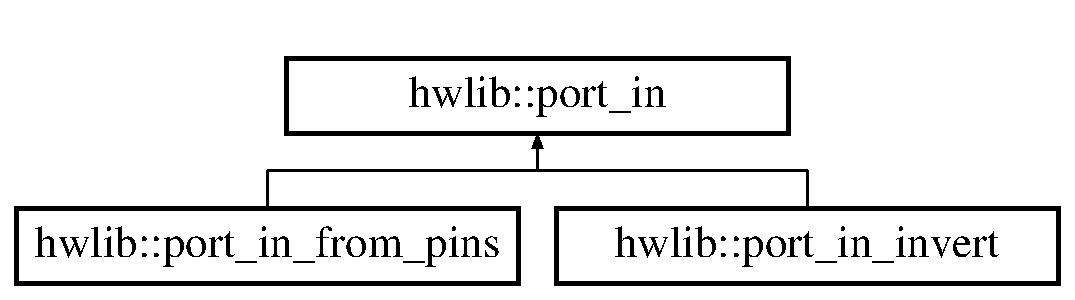
\includegraphics[height=2.000000cm]{classhwlib_1_1port__in}
\end{center}
\end{figure}
\subsection*{Public Member Functions}
\begin{DoxyCompactItemize}
\item 
virtual uint\+\_\+fast8\+\_\+t \hyperlink{classhwlib_1_1port__in_a3498fc0158e1e460a00d671df629fe22}{number\+\_\+of\+\_\+pins} ()=0
\begin{DoxyCompactList}\small\item\em get number of pins \end{DoxyCompactList}\item 
virtual uint\+\_\+fast8\+\_\+t \hyperlink{classhwlib_1_1port__in_a3c0a1346a61c538424048b61c1038e0c}{get} ()=0
\begin{DoxyCompactList}\small\item\em read from the port \end{DoxyCompactList}\end{DoxyCompactItemize}


\subsection{Detailed Description}
input port interface 

This is the interface of an input-\/only port. 

\subsection{Member Function Documentation}
\index{hwlib\+::port\+\_\+in@{hwlib\+::port\+\_\+in}!get@{get}}
\index{get@{get}!hwlib\+::port\+\_\+in@{hwlib\+::port\+\_\+in}}
\subsubsection[{\texorpdfstring{get()=0}{get()=0}}]{\setlength{\rightskip}{0pt plus 5cm}virtual uint\+\_\+fast8\+\_\+t hwlib\+::port\+\_\+in\+::get (
\begin{DoxyParamCaption}
{}
\end{DoxyParamCaption}
)\hspace{0.3cm}{\ttfamily [pure virtual]}}\hypertarget{classhwlib_1_1port__in_a3c0a1346a61c538424048b61c1038e0c}{}\label{classhwlib_1_1port__in_a3c0a1346a61c538424048b61c1038e0c}


read from the port 

This function reads and returns the pins that are part of the port. The lowest bit of the result reflects the first pin of the port, etc. 

Implemented in \hyperlink{classhwlib_1_1port__in__invert_a3100bd433a45e903894f5971ac958459}{hwlib\+::port\+\_\+in\+\_\+invert}, and \hyperlink{classhwlib_1_1port__in__from__pins_af137729dd87345ceb643b9dad3d6d274}{hwlib\+::port\+\_\+in\+\_\+from\+\_\+pins}.

\index{hwlib\+::port\+\_\+in@{hwlib\+::port\+\_\+in}!number\+\_\+of\+\_\+pins@{number\+\_\+of\+\_\+pins}}
\index{number\+\_\+of\+\_\+pins@{number\+\_\+of\+\_\+pins}!hwlib\+::port\+\_\+in@{hwlib\+::port\+\_\+in}}
\subsubsection[{\texorpdfstring{number\+\_\+of\+\_\+pins()=0}{number_of_pins()=0}}]{\setlength{\rightskip}{0pt plus 5cm}virtual uint\+\_\+fast8\+\_\+t hwlib\+::port\+\_\+in\+::number\+\_\+of\+\_\+pins (
\begin{DoxyParamCaption}
{}
\end{DoxyParamCaption}
)\hspace{0.3cm}{\ttfamily [pure virtual]}}\hypertarget{classhwlib_1_1port__in_a3498fc0158e1e460a00d671df629fe22}{}\label{classhwlib_1_1port__in_a3498fc0158e1e460a00d671df629fe22}


get number of pins 

This function returns the number of pins in the port. 

Implemented in \hyperlink{classhwlib_1_1port__in__invert_a5d05a4afd9990491daee8daa4c048faf}{hwlib\+::port\+\_\+in\+\_\+invert}, and \hyperlink{classhwlib_1_1port__in__from__pins_a7221f55f0bcee8b8aa56203141c90716}{hwlib\+::port\+\_\+in\+\_\+from\+\_\+pins}.



The documentation for this class was generated from the following file\+:\begin{DoxyCompactItemize}
\item 
\hyperlink{hwlib-port_8hpp}{hwlib-\/port.\+hpp}\end{DoxyCompactItemize}

\hypertarget{classhwlib_1_1port__in__from__pins}{}\section{hwlib\+:\+:port\+\_\+in\+\_\+from\+\_\+pins Class Reference}
\label{classhwlib_1_1port__in__from__pins}\index{hwlib\+::port\+\_\+in\+\_\+from\+\_\+pins@{hwlib\+::port\+\_\+in\+\_\+from\+\_\+pins}}


input port from input pins  




{\ttfamily \#include $<$hwlib-\/port.\+hpp$>$}

Inheritance diagram for hwlib\+:\+:port\+\_\+in\+\_\+from\+\_\+pins\+:\begin{figure}[H]
\begin{center}
\leavevmode
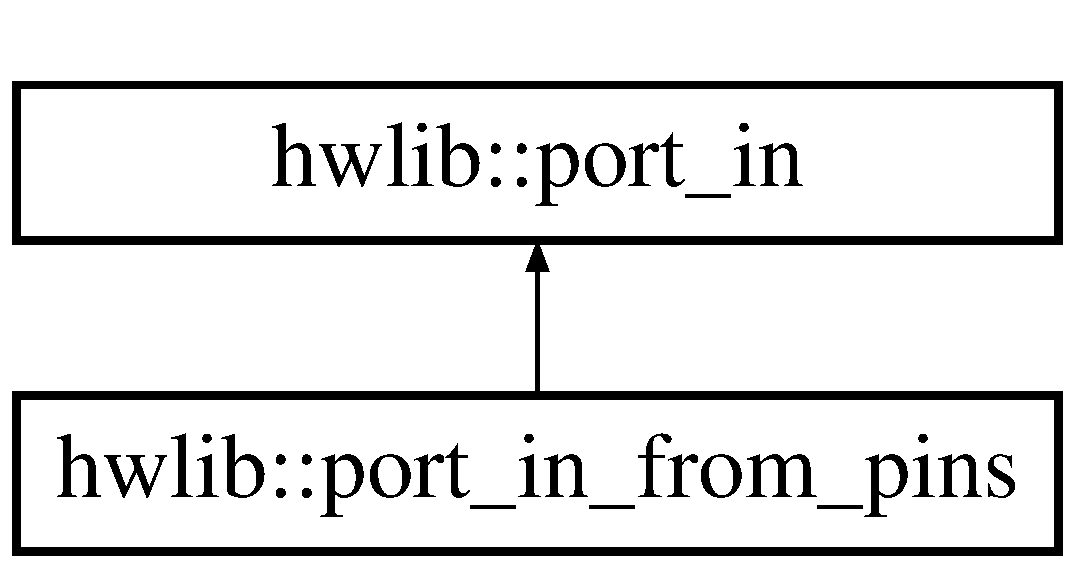
\includegraphics[height=2.000000cm]{classhwlib_1_1port__in__from__pins}
\end{center}
\end{figure}
\subsection*{Public Member Functions}
\begin{DoxyCompactItemize}
\item 
\hyperlink{classhwlib_1_1port__in__from__pins_ab7193755e6819043946e90f1dfafd70f}{port\+\_\+in\+\_\+from\+\_\+pins} (\hyperlink{classhwlib_1_1pin__in}{pin\+\_\+in} \&p0=pin\+\_\+in\+\_\+dummy, \hyperlink{classhwlib_1_1pin__in}{pin\+\_\+in} \&p1=pin\+\_\+in\+\_\+dummy, \hyperlink{classhwlib_1_1pin__in}{pin\+\_\+in} \&p2=pin\+\_\+in\+\_\+dummy, \hyperlink{classhwlib_1_1pin__in}{pin\+\_\+in} \&p3=pin\+\_\+in\+\_\+dummy, \hyperlink{classhwlib_1_1pin__in}{pin\+\_\+in} \&p4=pin\+\_\+in\+\_\+dummy, \hyperlink{classhwlib_1_1pin__in}{pin\+\_\+in} \&p5=pin\+\_\+in\+\_\+dummy, \hyperlink{classhwlib_1_1pin__in}{pin\+\_\+in} \&p6=pin\+\_\+in\+\_\+dummy, \hyperlink{classhwlib_1_1pin__in}{pin\+\_\+in} \&p7=pin\+\_\+in\+\_\+dummy)
\begin{DoxyCompactList}\small\item\em construct a \hyperlink{classhwlib_1_1port__out}{port\+\_\+out} from up to 8 pin\+\_\+outs \end{DoxyCompactList}\item 
uint\+\_\+fast8\+\_\+t \hyperlink{classhwlib_1_1port__in__from__pins_a7221f55f0bcee8b8aa56203141c90716}{number\+\_\+of\+\_\+pins} () override
\begin{DoxyCompactList}\small\item\em get number of pins \end{DoxyCompactList}\item 
uint\+\_\+fast8\+\_\+t \hyperlink{classhwlib_1_1port__in__from__pins_af137729dd87345ceb643b9dad3d6d274}{get} () override
\begin{DoxyCompactList}\small\item\em read from the port \end{DoxyCompactList}\end{DoxyCompactItemize}


\subsection{Detailed Description}
input port from input pins 

This class implements an input-\/only port made from port up to 8 pins. 

\subsection{Constructor \& Destructor Documentation}
\index{hwlib\+::port\+\_\+in\+\_\+from\+\_\+pins@{hwlib\+::port\+\_\+in\+\_\+from\+\_\+pins}!port\+\_\+in\+\_\+from\+\_\+pins@{port\+\_\+in\+\_\+from\+\_\+pins}}
\index{port\+\_\+in\+\_\+from\+\_\+pins@{port\+\_\+in\+\_\+from\+\_\+pins}!hwlib\+::port\+\_\+in\+\_\+from\+\_\+pins@{hwlib\+::port\+\_\+in\+\_\+from\+\_\+pins}}
\subsubsection[{\texorpdfstring{port\+\_\+in\+\_\+from\+\_\+pins(pin\+\_\+in \&p0=pin\+\_\+in\+\_\+dummy, pin\+\_\+in \&p1=pin\+\_\+in\+\_\+dummy, pin\+\_\+in \&p2=pin\+\_\+in\+\_\+dummy, pin\+\_\+in \&p3=pin\+\_\+in\+\_\+dummy, pin\+\_\+in \&p4=pin\+\_\+in\+\_\+dummy, pin\+\_\+in \&p5=pin\+\_\+in\+\_\+dummy, pin\+\_\+in \&p6=pin\+\_\+in\+\_\+dummy, pin\+\_\+in \&p7=pin\+\_\+in\+\_\+dummy)}{port_in_from_pins(pin_in &p0=pin_in_dummy, pin_in &p1=pin_in_dummy, pin_in &p2=pin_in_dummy, pin_in &p3=pin_in_dummy, pin_in &p4=pin_in_dummy, pin_in &p5=pin_in_dummy, pin_in &p6=pin_in_dummy, pin_in &p7=pin_in_dummy)}}]{\setlength{\rightskip}{0pt plus 5cm}hwlib\+::port\+\_\+in\+\_\+from\+\_\+pins\+::port\+\_\+in\+\_\+from\+\_\+pins (
\begin{DoxyParamCaption}
\item[{{\bf pin\+\_\+in} \&}]{p0 = {\ttfamily pin\+\_\+in\+\_\+dummy}, }
\item[{{\bf pin\+\_\+in} \&}]{p1 = {\ttfamily pin\+\_\+in\+\_\+dummy}, }
\item[{{\bf pin\+\_\+in} \&}]{p2 = {\ttfamily pin\+\_\+in\+\_\+dummy}, }
\item[{{\bf pin\+\_\+in} \&}]{p3 = {\ttfamily pin\+\_\+in\+\_\+dummy}, }
\item[{{\bf pin\+\_\+in} \&}]{p4 = {\ttfamily pin\+\_\+in\+\_\+dummy}, }
\item[{{\bf pin\+\_\+in} \&}]{p5 = {\ttfamily pin\+\_\+in\+\_\+dummy}, }
\item[{{\bf pin\+\_\+in} \&}]{p6 = {\ttfamily pin\+\_\+in\+\_\+dummy}, }
\item[{{\bf pin\+\_\+in} \&}]{p7 = {\ttfamily pin\+\_\+in\+\_\+dummy}}
\end{DoxyParamCaption}
)\hspace{0.3cm}{\ttfamily [inline]}}\hypertarget{classhwlib_1_1port__in__from__pins_ab7193755e6819043946e90f1dfafd70f}{}\label{classhwlib_1_1port__in__from__pins_ab7193755e6819043946e90f1dfafd70f}


construct a \hyperlink{classhwlib_1_1port__out}{port\+\_\+out} from up to 8 pin\+\_\+outs 

This constructor creates a \hyperlink{classhwlib_1_1port__out}{port\+\_\+out} from up to 8 \hyperlink{classhwlib_1_1pin__in}{pin\+\_\+in} pins. The first pin is the lowest pin in the port, etc. 

\subsection{Member Function Documentation}
\index{hwlib\+::port\+\_\+in\+\_\+from\+\_\+pins@{hwlib\+::port\+\_\+in\+\_\+from\+\_\+pins}!get@{get}}
\index{get@{get}!hwlib\+::port\+\_\+in\+\_\+from\+\_\+pins@{hwlib\+::port\+\_\+in\+\_\+from\+\_\+pins}}
\subsubsection[{\texorpdfstring{get() override}{get() override}}]{\setlength{\rightskip}{0pt plus 5cm}uint\+\_\+fast8\+\_\+t hwlib\+::port\+\_\+in\+\_\+from\+\_\+pins\+::get (
\begin{DoxyParamCaption}
{}
\end{DoxyParamCaption}
)\hspace{0.3cm}{\ttfamily [inline]}, {\ttfamily [override]}, {\ttfamily [virtual]}}\hypertarget{classhwlib_1_1port__in__from__pins_af137729dd87345ceb643b9dad3d6d274}{}\label{classhwlib_1_1port__in__from__pins_af137729dd87345ceb643b9dad3d6d274}


read from the port 

This function reads and returns the pins that are part of the port. The lowest bit of the result reflects the first pin of the port, etc. 

Implements \hyperlink{classhwlib_1_1port__in_a3c0a1346a61c538424048b61c1038e0c}{hwlib\+::port\+\_\+in}.

\index{hwlib\+::port\+\_\+in\+\_\+from\+\_\+pins@{hwlib\+::port\+\_\+in\+\_\+from\+\_\+pins}!number\+\_\+of\+\_\+pins@{number\+\_\+of\+\_\+pins}}
\index{number\+\_\+of\+\_\+pins@{number\+\_\+of\+\_\+pins}!hwlib\+::port\+\_\+in\+\_\+from\+\_\+pins@{hwlib\+::port\+\_\+in\+\_\+from\+\_\+pins}}
\subsubsection[{\texorpdfstring{number\+\_\+of\+\_\+pins() override}{number_of_pins() override}}]{\setlength{\rightskip}{0pt plus 5cm}uint\+\_\+fast8\+\_\+t hwlib\+::port\+\_\+in\+\_\+from\+\_\+pins\+::number\+\_\+of\+\_\+pins (
\begin{DoxyParamCaption}
{}
\end{DoxyParamCaption}
)\hspace{0.3cm}{\ttfamily [inline]}, {\ttfamily [override]}, {\ttfamily [virtual]}}\hypertarget{classhwlib_1_1port__in__from__pins_a7221f55f0bcee8b8aa56203141c90716}{}\label{classhwlib_1_1port__in__from__pins_a7221f55f0bcee8b8aa56203141c90716}


get number of pins 

This function returns the number of pins in the port. 

Implements \hyperlink{classhwlib_1_1port__in_a3498fc0158e1e460a00d671df629fe22}{hwlib\+::port\+\_\+in}.



The documentation for this class was generated from the following file\+:\begin{DoxyCompactItemize}
\item 
\hyperlink{hwlib-port_8hpp}{hwlib-\/port.\+hpp}\end{DoxyCompactItemize}

\hypertarget{classhwlib_1_1port__in__invert}{}\section{hwlib\+:\+:port\+\_\+in\+\_\+invert Class Reference}
\label{classhwlib_1_1port__in__invert}\index{hwlib\+::port\+\_\+in\+\_\+invert@{hwlib\+::port\+\_\+in\+\_\+invert}}


invert an input port  




{\ttfamily \#include $<$hwlib-\/port.\+hpp$>$}

Inheritance diagram for hwlib\+:\+:port\+\_\+in\+\_\+invert\+:\begin{figure}[H]
\begin{center}
\leavevmode
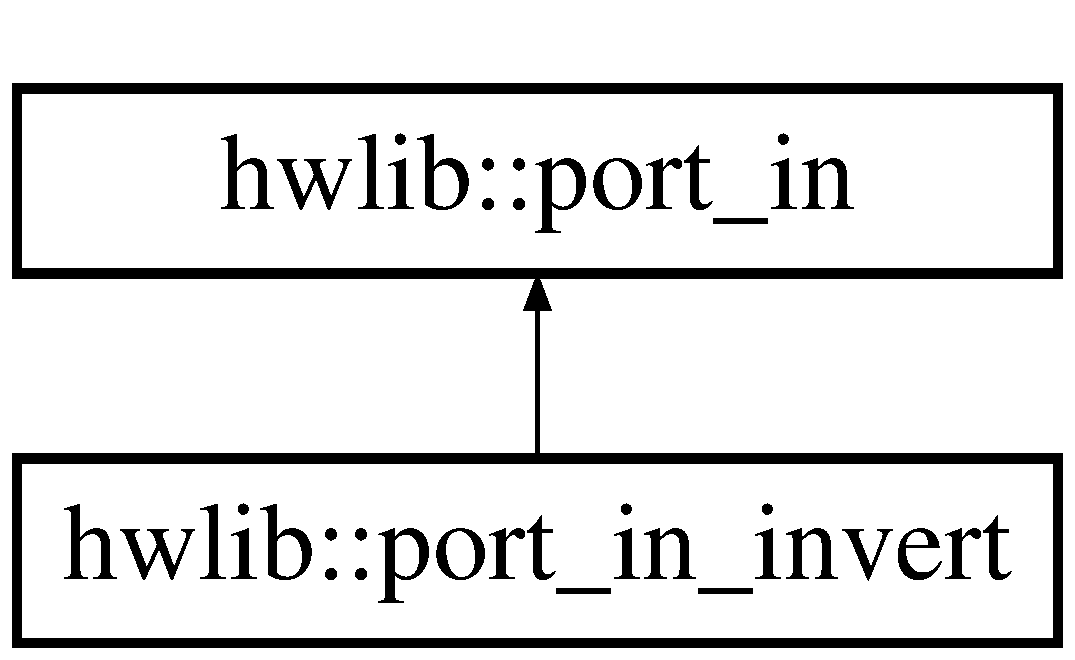
\includegraphics[height=2.000000cm]{classhwlib_1_1port__in__invert}
\end{center}
\end{figure}
\subsection*{Public Member Functions}
\begin{DoxyCompactItemize}
\item 
\hyperlink{classhwlib_1_1port__in__invert_afdf7f63dbf6c202b801742f50b6f5017}{port\+\_\+in\+\_\+invert} (\hyperlink{classhwlib_1_1port__in}{port\+\_\+in} \&port)
\begin{DoxyCompactList}\small\item\em construct an inverted input port \end{DoxyCompactList}\item 
uint\+\_\+fast8\+\_\+t \hyperlink{classhwlib_1_1port__in__invert_a5d05a4afd9990491daee8daa4c048faf}{number\+\_\+of\+\_\+pins} () override
\begin{DoxyCompactList}\small\item\em get number of pins \end{DoxyCompactList}\item 
uint\+\_\+fast8\+\_\+t \hyperlink{classhwlib_1_1port__in__invert_a3100bd433a45e903894f5971ac958459}{get} () override
\begin{DoxyCompactList}\small\item\em read from the port \end{DoxyCompactList}\end{DoxyCompactItemize}


\subsection{Detailed Description}
invert an input port 

This decorator inverts the result of read operations on an input port\+: When a value would be returned by the original port, the inverted port returns the value with all bits inverted. 

\subsection{Constructor \& Destructor Documentation}
\index{hwlib\+::port\+\_\+in\+\_\+invert@{hwlib\+::port\+\_\+in\+\_\+invert}!port\+\_\+in\+\_\+invert@{port\+\_\+in\+\_\+invert}}
\index{port\+\_\+in\+\_\+invert@{port\+\_\+in\+\_\+invert}!hwlib\+::port\+\_\+in\+\_\+invert@{hwlib\+::port\+\_\+in\+\_\+invert}}
\subsubsection[{\texorpdfstring{port\+\_\+in\+\_\+invert(port\+\_\+in \&port)}{port_in_invert(port_in &port)}}]{\setlength{\rightskip}{0pt plus 5cm}hwlib\+::port\+\_\+in\+\_\+invert\+::port\+\_\+in\+\_\+invert (
\begin{DoxyParamCaption}
\item[{{\bf port\+\_\+in} \&}]{port}
\end{DoxyParamCaption}
)\hspace{0.3cm}{\ttfamily [inline]}}\hypertarget{classhwlib_1_1port__in__invert_afdf7f63dbf6c202b801742f50b6f5017}{}\label{classhwlib_1_1port__in__invert_afdf7f63dbf6c202b801742f50b6f5017}


construct an inverted input port 

This constructor creates an inverted input port from an existing input port. 

\subsection{Member Function Documentation}
\index{hwlib\+::port\+\_\+in\+\_\+invert@{hwlib\+::port\+\_\+in\+\_\+invert}!get@{get}}
\index{get@{get}!hwlib\+::port\+\_\+in\+\_\+invert@{hwlib\+::port\+\_\+in\+\_\+invert}}
\subsubsection[{\texorpdfstring{get() override}{get() override}}]{\setlength{\rightskip}{0pt plus 5cm}uint\+\_\+fast8\+\_\+t hwlib\+::port\+\_\+in\+\_\+invert\+::get (
\begin{DoxyParamCaption}
{}
\end{DoxyParamCaption}
)\hspace{0.3cm}{\ttfamily [inline]}, {\ttfamily [override]}, {\ttfamily [virtual]}}\hypertarget{classhwlib_1_1port__in__invert_a3100bd433a45e903894f5971ac958459}{}\label{classhwlib_1_1port__in__invert_a3100bd433a45e903894f5971ac958459}


read from the port 

This function reads and returns the pins that are part of the port. The lowest bit of the result reflects the first pin of the port, etc. 

Implements \hyperlink{classhwlib_1_1port__in_a3c0a1346a61c538424048b61c1038e0c}{hwlib\+::port\+\_\+in}.

\index{hwlib\+::port\+\_\+in\+\_\+invert@{hwlib\+::port\+\_\+in\+\_\+invert}!number\+\_\+of\+\_\+pins@{number\+\_\+of\+\_\+pins}}
\index{number\+\_\+of\+\_\+pins@{number\+\_\+of\+\_\+pins}!hwlib\+::port\+\_\+in\+\_\+invert@{hwlib\+::port\+\_\+in\+\_\+invert}}
\subsubsection[{\texorpdfstring{number\+\_\+of\+\_\+pins() override}{number_of_pins() override}}]{\setlength{\rightskip}{0pt plus 5cm}uint\+\_\+fast8\+\_\+t hwlib\+::port\+\_\+in\+\_\+invert\+::number\+\_\+of\+\_\+pins (
\begin{DoxyParamCaption}
{}
\end{DoxyParamCaption}
)\hspace{0.3cm}{\ttfamily [inline]}, {\ttfamily [override]}, {\ttfamily [virtual]}}\hypertarget{classhwlib_1_1port__in__invert_a5d05a4afd9990491daee8daa4c048faf}{}\label{classhwlib_1_1port__in__invert_a5d05a4afd9990491daee8daa4c048faf}


get number of pins 

This function returns the number of pins in the port. 

Implements \hyperlink{classhwlib_1_1port__in_a3498fc0158e1e460a00d671df629fe22}{hwlib\+::port\+\_\+in}.



The documentation for this class was generated from the following file\+:\begin{DoxyCompactItemize}
\item 
\hyperlink{hwlib-port_8hpp}{hwlib-\/port.\+hpp}\end{DoxyCompactItemize}

\hypertarget{classhwlib_1_1port__in__out}{}\section{hwlib\+:\+:port\+\_\+in\+\_\+out Class Reference}
\label{classhwlib_1_1port__in__out}\index{hwlib\+::port\+\_\+in\+\_\+out@{hwlib\+::port\+\_\+in\+\_\+out}}


input / output port interface  




{\ttfamily \#include $<$hwlib-\/port.\+hpp$>$}

Inheritance diagram for hwlib\+:\+:port\+\_\+in\+\_\+out\+:\begin{figure}[H]
\begin{center}
\leavevmode
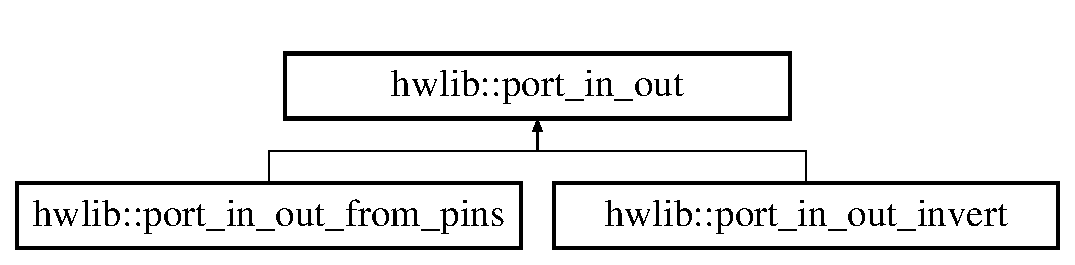
\includegraphics[height=2.000000cm]{classhwlib_1_1port__in__out}
\end{center}
\end{figure}
\subsection*{Public Member Functions}
\begin{DoxyCompactItemize}
\item 
virtual uint\+\_\+fast8\+\_\+t \hyperlink{classhwlib_1_1port__in__out_a44243a6c7664e734563f1809058751bc}{number\+\_\+of\+\_\+pins} ()=0
\begin{DoxyCompactList}\small\item\em get number of pins \end{DoxyCompactList}\item 
virtual void \hyperlink{classhwlib_1_1port__in__out_ac7a9611410ddb9fd5d8e2dd15bff0a3f}{direction\+\_\+set\+\_\+input} ()=0
\begin{DoxyCompactList}\small\item\em set the direction of the port to input. \end{DoxyCompactList}\item 
virtual uint\+\_\+fast8\+\_\+t \hyperlink{classhwlib_1_1port__in__out_a822b44b3dd5b9df225e793896aeba641}{get} ()=0
\begin{DoxyCompactList}\small\item\em read from the port \end{DoxyCompactList}\item 
virtual void \hyperlink{classhwlib_1_1port__in__out_a515b4a6bbde4f2df5bb11cda41234fe4}{direction\+\_\+set\+\_\+output} ()=0
\begin{DoxyCompactList}\small\item\em set the direction of the port to output \end{DoxyCompactList}\item 
virtual void \hyperlink{classhwlib_1_1port__in__out_adaca419a61193e42e06e52afbbc4afe4}{set} (uint\+\_\+fast8\+\_\+t x)=0
\begin{DoxyCompactList}\small\item\em write to the port \end{DoxyCompactList}\end{DoxyCompactItemize}


\subsection{Detailed Description}
input / output port interface 

This is the interface of an input / output port. 

\subsection{Member Function Documentation}
\index{hwlib\+::port\+\_\+in\+\_\+out@{hwlib\+::port\+\_\+in\+\_\+out}!direction\+\_\+set\+\_\+input@{direction\+\_\+set\+\_\+input}}
\index{direction\+\_\+set\+\_\+input@{direction\+\_\+set\+\_\+input}!hwlib\+::port\+\_\+in\+\_\+out@{hwlib\+::port\+\_\+in\+\_\+out}}
\subsubsection[{\texorpdfstring{direction\+\_\+set\+\_\+input()=0}{direction_set_input()=0}}]{\setlength{\rightskip}{0pt plus 5cm}virtual void hwlib\+::port\+\_\+in\+\_\+out\+::direction\+\_\+set\+\_\+input (
\begin{DoxyParamCaption}
{}
\end{DoxyParamCaption}
)\hspace{0.3cm}{\ttfamily [pure virtual]}}\hypertarget{classhwlib_1_1port__in__out_ac7a9611410ddb9fd5d8e2dd15bff0a3f}{}\label{classhwlib_1_1port__in__out_ac7a9611410ddb9fd5d8e2dd15bff0a3f}


set the direction of the port to input. 

Calling this function sets all pins of the port to input. 

Implemented in \hyperlink{classhwlib_1_1port__in__out__invert_aa9a02e447e2d960e8013300e4a06a35a}{hwlib\+::port\+\_\+in\+\_\+out\+\_\+invert}, and \hyperlink{classhwlib_1_1port__in__out__from__pins_a63dda73defa40b64d61caff9e3209c95}{hwlib\+::port\+\_\+in\+\_\+out\+\_\+from\+\_\+pins}.

\index{hwlib\+::port\+\_\+in\+\_\+out@{hwlib\+::port\+\_\+in\+\_\+out}!direction\+\_\+set\+\_\+output@{direction\+\_\+set\+\_\+output}}
\index{direction\+\_\+set\+\_\+output@{direction\+\_\+set\+\_\+output}!hwlib\+::port\+\_\+in\+\_\+out@{hwlib\+::port\+\_\+in\+\_\+out}}
\subsubsection[{\texorpdfstring{direction\+\_\+set\+\_\+output()=0}{direction_set_output()=0}}]{\setlength{\rightskip}{0pt plus 5cm}virtual void hwlib\+::port\+\_\+in\+\_\+out\+::direction\+\_\+set\+\_\+output (
\begin{DoxyParamCaption}
{}
\end{DoxyParamCaption}
)\hspace{0.3cm}{\ttfamily [pure virtual]}}\hypertarget{classhwlib_1_1port__in__out_a515b4a6bbde4f2df5bb11cda41234fe4}{}\label{classhwlib_1_1port__in__out_a515b4a6bbde4f2df5bb11cda41234fe4}


set the direction of the port to output 

Calling this function sets all pins of the port to output. 

Implemented in \hyperlink{classhwlib_1_1port__in__out__invert_a038aeaafb573ef871d3608d489977a17}{hwlib\+::port\+\_\+in\+\_\+out\+\_\+invert}, and \hyperlink{classhwlib_1_1port__in__out__from__pins_a82d271d0bd20b627c5ebf250ad3f844e}{hwlib\+::port\+\_\+in\+\_\+out\+\_\+from\+\_\+pins}.

\index{hwlib\+::port\+\_\+in\+\_\+out@{hwlib\+::port\+\_\+in\+\_\+out}!get@{get}}
\index{get@{get}!hwlib\+::port\+\_\+in\+\_\+out@{hwlib\+::port\+\_\+in\+\_\+out}}
\subsubsection[{\texorpdfstring{get()=0}{get()=0}}]{\setlength{\rightskip}{0pt plus 5cm}virtual uint\+\_\+fast8\+\_\+t hwlib\+::port\+\_\+in\+\_\+out\+::get (
\begin{DoxyParamCaption}
{}
\end{DoxyParamCaption}
)\hspace{0.3cm}{\ttfamily [pure virtual]}}\hypertarget{classhwlib_1_1port__in__out_a822b44b3dd5b9df225e793896aeba641}{}\label{classhwlib_1_1port__in__out_a822b44b3dd5b9df225e793896aeba641}


read from the port 

This function reads and returns the pins that are part of the port. The lowest bit of the result reflects the first pin of the port, etc.

Before calling this function the port direction must have been set to input by calling port\+\_\+direction\+\_\+set\+\_\+input(). 

Implemented in \hyperlink{classhwlib_1_1port__in__out__invert_ae7fac086fb1203b68376ec77a38e6187}{hwlib\+::port\+\_\+in\+\_\+out\+\_\+invert}, and \hyperlink{classhwlib_1_1port__in__out__from__pins_a5b8af7271d9fd08b005bc33ddada3cbe}{hwlib\+::port\+\_\+in\+\_\+out\+\_\+from\+\_\+pins}.

\index{hwlib\+::port\+\_\+in\+\_\+out@{hwlib\+::port\+\_\+in\+\_\+out}!number\+\_\+of\+\_\+pins@{number\+\_\+of\+\_\+pins}}
\index{number\+\_\+of\+\_\+pins@{number\+\_\+of\+\_\+pins}!hwlib\+::port\+\_\+in\+\_\+out@{hwlib\+::port\+\_\+in\+\_\+out}}
\subsubsection[{\texorpdfstring{number\+\_\+of\+\_\+pins()=0}{number_of_pins()=0}}]{\setlength{\rightskip}{0pt plus 5cm}virtual uint\+\_\+fast8\+\_\+t hwlib\+::port\+\_\+in\+\_\+out\+::number\+\_\+of\+\_\+pins (
\begin{DoxyParamCaption}
{}
\end{DoxyParamCaption}
)\hspace{0.3cm}{\ttfamily [pure virtual]}}\hypertarget{classhwlib_1_1port__in__out_a44243a6c7664e734563f1809058751bc}{}\label{classhwlib_1_1port__in__out_a44243a6c7664e734563f1809058751bc}


get number of pins 

This function returns the number of pins in the port. 

Implemented in \hyperlink{classhwlib_1_1port__in__out__invert_a8f3facb156f79e209a2db42b168edd46}{hwlib\+::port\+\_\+in\+\_\+out\+\_\+invert}, and \hyperlink{classhwlib_1_1port__in__out__from__pins_a7e5e5767a4d104461939e0b7c5dd8482}{hwlib\+::port\+\_\+in\+\_\+out\+\_\+from\+\_\+pins}.

\index{hwlib\+::port\+\_\+in\+\_\+out@{hwlib\+::port\+\_\+in\+\_\+out}!set@{set}}
\index{set@{set}!hwlib\+::port\+\_\+in\+\_\+out@{hwlib\+::port\+\_\+in\+\_\+out}}
\subsubsection[{\texorpdfstring{set(uint\+\_\+fast8\+\_\+t x)=0}{set(uint_fast8_t x)=0}}]{\setlength{\rightskip}{0pt plus 5cm}virtual void hwlib\+::port\+\_\+in\+\_\+out\+::set (
\begin{DoxyParamCaption}
\item[{uint\+\_\+fast8\+\_\+t}]{x}
\end{DoxyParamCaption}
)\hspace{0.3cm}{\ttfamily [pure virtual]}}\hypertarget{classhwlib_1_1port__in__out_adaca419a61193e42e06e52afbbc4afe4}{}\label{classhwlib_1_1port__in__out_adaca419a61193e42e06e52afbbc4afe4}


write to the port 

This function writes to the pins that are part of the port. The lowest bit is written to the first pin of the port, etc.

Before calling this function the port direction must have been set to output by calling \hyperlink{classhwlib_1_1port__in__out_a515b4a6bbde4f2df5bb11cda41234fe4}{direction\+\_\+set\+\_\+output()}. 

Implemented in \hyperlink{classhwlib_1_1port__in__out__invert_ac2d24269e7fd164fa3d32c4ead0bc6c7}{hwlib\+::port\+\_\+in\+\_\+out\+\_\+invert}, and \hyperlink{classhwlib_1_1port__in__out__from__pins_a6c2bbeca500638cb35f142e8f74bf857}{hwlib\+::port\+\_\+in\+\_\+out\+\_\+from\+\_\+pins}.



The documentation for this class was generated from the following file\+:\begin{DoxyCompactItemize}
\item 
\hyperlink{hwlib-port_8hpp}{hwlib-\/port.\+hpp}\end{DoxyCompactItemize}

\hypertarget{classhwlib_1_1port__in__out__from__pins}{}\section{hwlib\+:\+:port\+\_\+in\+\_\+out\+\_\+from\+\_\+pins Class Reference}
\label{classhwlib_1_1port__in__out__from__pins}\index{hwlib\+::port\+\_\+in\+\_\+out\+\_\+from\+\_\+pins@{hwlib\+::port\+\_\+in\+\_\+out\+\_\+from\+\_\+pins}}


input/output port from input/output pins  




{\ttfamily \#include $<$hwlib-\/port.\+hpp$>$}

Inheritance diagram for hwlib\+:\+:port\+\_\+in\+\_\+out\+\_\+from\+\_\+pins\+:\begin{figure}[H]
\begin{center}
\leavevmode
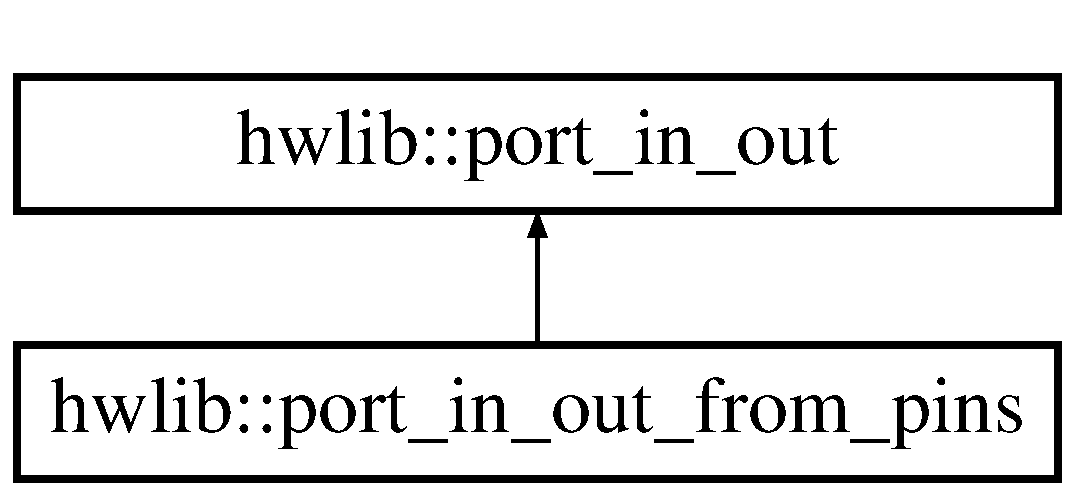
\includegraphics[height=2.000000cm]{classhwlib_1_1port__in__out__from__pins}
\end{center}
\end{figure}
\subsection*{Public Member Functions}
\begin{DoxyCompactItemize}
\item 
\hyperlink{classhwlib_1_1port__in__out__from__pins_a69cc74af76d03ff9008e7f130b7065ee}{port\+\_\+in\+\_\+out\+\_\+from\+\_\+pins} (\hyperlink{classhwlib_1_1pin__in__out}{pin\+\_\+in\+\_\+out} \&p0=pin\+\_\+in\+\_\+out\+\_\+dummy, \hyperlink{classhwlib_1_1pin__in__out}{pin\+\_\+in\+\_\+out} \&p1=pin\+\_\+in\+\_\+out\+\_\+dummy, \hyperlink{classhwlib_1_1pin__in__out}{pin\+\_\+in\+\_\+out} \&p2=pin\+\_\+in\+\_\+out\+\_\+dummy, \hyperlink{classhwlib_1_1pin__in__out}{pin\+\_\+in\+\_\+out} \&p3=pin\+\_\+in\+\_\+out\+\_\+dummy, \hyperlink{classhwlib_1_1pin__in__out}{pin\+\_\+in\+\_\+out} \&p4=pin\+\_\+in\+\_\+out\+\_\+dummy, \hyperlink{classhwlib_1_1pin__in__out}{pin\+\_\+in\+\_\+out} \&p5=pin\+\_\+in\+\_\+out\+\_\+dummy, \hyperlink{classhwlib_1_1pin__in__out}{pin\+\_\+in\+\_\+out} \&p6=pin\+\_\+in\+\_\+out\+\_\+dummy, \hyperlink{classhwlib_1_1pin__in__out}{pin\+\_\+in\+\_\+out} \&p7=pin\+\_\+in\+\_\+out\+\_\+dummy)
\begin{DoxyCompactList}\small\item\em construct a \hyperlink{classhwlib_1_1port__out}{port\+\_\+out} from up to 8 pin\+\_\+outs \end{DoxyCompactList}\item 
uint\+\_\+fast8\+\_\+t \hyperlink{classhwlib_1_1port__in__out__from__pins_a7e5e5767a4d104461939e0b7c5dd8482}{number\+\_\+of\+\_\+pins} () override
\begin{DoxyCompactList}\small\item\em get number of pins \end{DoxyCompactList}\item 
void \hyperlink{classhwlib_1_1port__in__out__from__pins_a63dda73defa40b64d61caff9e3209c95}{direction\+\_\+set\+\_\+input} () override
\begin{DoxyCompactList}\small\item\em set the direction of the port to input. \end{DoxyCompactList}\item 
void \hyperlink{classhwlib_1_1port__in__out__from__pins_a82d271d0bd20b627c5ebf250ad3f844e}{direction\+\_\+set\+\_\+output} () override
\begin{DoxyCompactList}\small\item\em set the direction of the port to output \end{DoxyCompactList}\item 
uint\+\_\+fast8\+\_\+t \hyperlink{classhwlib_1_1port__in__out__from__pins_a5b8af7271d9fd08b005bc33ddada3cbe}{get} () override
\begin{DoxyCompactList}\small\item\em read from the port \end{DoxyCompactList}\item 
void \hyperlink{classhwlib_1_1port__in__out__from__pins_a6c2bbeca500638cb35f142e8f74bf857}{set} (uint\+\_\+fast8\+\_\+t x) override
\begin{DoxyCompactList}\small\item\em write to the port \end{DoxyCompactList}\end{DoxyCompactItemize}


\subsection{Detailed Description}
input/output port from input/output pins 

This class implements an input/output port made from port up to 8 pins. 

\subsection{Constructor \& Destructor Documentation}
\index{hwlib\+::port\+\_\+in\+\_\+out\+\_\+from\+\_\+pins@{hwlib\+::port\+\_\+in\+\_\+out\+\_\+from\+\_\+pins}!port\+\_\+in\+\_\+out\+\_\+from\+\_\+pins@{port\+\_\+in\+\_\+out\+\_\+from\+\_\+pins}}
\index{port\+\_\+in\+\_\+out\+\_\+from\+\_\+pins@{port\+\_\+in\+\_\+out\+\_\+from\+\_\+pins}!hwlib\+::port\+\_\+in\+\_\+out\+\_\+from\+\_\+pins@{hwlib\+::port\+\_\+in\+\_\+out\+\_\+from\+\_\+pins}}
\subsubsection[{\texorpdfstring{port\+\_\+in\+\_\+out\+\_\+from\+\_\+pins(pin\+\_\+in\+\_\+out \&p0=pin\+\_\+in\+\_\+out\+\_\+dummy, pin\+\_\+in\+\_\+out \&p1=pin\+\_\+in\+\_\+out\+\_\+dummy, pin\+\_\+in\+\_\+out \&p2=pin\+\_\+in\+\_\+out\+\_\+dummy, pin\+\_\+in\+\_\+out \&p3=pin\+\_\+in\+\_\+out\+\_\+dummy, pin\+\_\+in\+\_\+out \&p4=pin\+\_\+in\+\_\+out\+\_\+dummy, pin\+\_\+in\+\_\+out \&p5=pin\+\_\+in\+\_\+out\+\_\+dummy, pin\+\_\+in\+\_\+out \&p6=pin\+\_\+in\+\_\+out\+\_\+dummy, pin\+\_\+in\+\_\+out \&p7=pin\+\_\+in\+\_\+out\+\_\+dummy)}{port_in_out_from_pins(pin_in_out &p0=pin_in_out_dummy, pin_in_out &p1=pin_in_out_dummy, pin_in_out &p2=pin_in_out_dummy, pin_in_out &p3=pin_in_out_dummy, pin_in_out &p4=pin_in_out_dummy, pin_in_out &p5=pin_in_out_dummy, pin_in_out &p6=pin_in_out_dummy, pin_in_out &p7=pin_in_out_dummy)}}]{\setlength{\rightskip}{0pt plus 5cm}hwlib\+::port\+\_\+in\+\_\+out\+\_\+from\+\_\+pins\+::port\+\_\+in\+\_\+out\+\_\+from\+\_\+pins (
\begin{DoxyParamCaption}
\item[{{\bf pin\+\_\+in\+\_\+out} \&}]{p0 = {\ttfamily pin\+\_\+in\+\_\+out\+\_\+dummy}, }
\item[{{\bf pin\+\_\+in\+\_\+out} \&}]{p1 = {\ttfamily pin\+\_\+in\+\_\+out\+\_\+dummy}, }
\item[{{\bf pin\+\_\+in\+\_\+out} \&}]{p2 = {\ttfamily pin\+\_\+in\+\_\+out\+\_\+dummy}, }
\item[{{\bf pin\+\_\+in\+\_\+out} \&}]{p3 = {\ttfamily pin\+\_\+in\+\_\+out\+\_\+dummy}, }
\item[{{\bf pin\+\_\+in\+\_\+out} \&}]{p4 = {\ttfamily pin\+\_\+in\+\_\+out\+\_\+dummy}, }
\item[{{\bf pin\+\_\+in\+\_\+out} \&}]{p5 = {\ttfamily pin\+\_\+in\+\_\+out\+\_\+dummy}, }
\item[{{\bf pin\+\_\+in\+\_\+out} \&}]{p6 = {\ttfamily pin\+\_\+in\+\_\+out\+\_\+dummy}, }
\item[{{\bf pin\+\_\+in\+\_\+out} \&}]{p7 = {\ttfamily pin\+\_\+in\+\_\+out\+\_\+dummy}}
\end{DoxyParamCaption}
)\hspace{0.3cm}{\ttfamily [inline]}}\hypertarget{classhwlib_1_1port__in__out__from__pins_a69cc74af76d03ff9008e7f130b7065ee}{}\label{classhwlib_1_1port__in__out__from__pins_a69cc74af76d03ff9008e7f130b7065ee}


construct a \hyperlink{classhwlib_1_1port__out}{port\+\_\+out} from up to 8 pin\+\_\+outs 

This constructor creates a \hyperlink{classhwlib_1_1port__out}{port\+\_\+out} from up to 8 \hyperlink{classhwlib_1_1pin__in}{pin\+\_\+in} pins. The first pin is the lowest pin in the port, etc. 

\subsection{Member Function Documentation}
\index{hwlib\+::port\+\_\+in\+\_\+out\+\_\+from\+\_\+pins@{hwlib\+::port\+\_\+in\+\_\+out\+\_\+from\+\_\+pins}!direction\+\_\+set\+\_\+input@{direction\+\_\+set\+\_\+input}}
\index{direction\+\_\+set\+\_\+input@{direction\+\_\+set\+\_\+input}!hwlib\+::port\+\_\+in\+\_\+out\+\_\+from\+\_\+pins@{hwlib\+::port\+\_\+in\+\_\+out\+\_\+from\+\_\+pins}}
\subsubsection[{\texorpdfstring{direction\+\_\+set\+\_\+input() override}{direction_set_input() override}}]{\setlength{\rightskip}{0pt plus 5cm}void hwlib\+::port\+\_\+in\+\_\+out\+\_\+from\+\_\+pins\+::direction\+\_\+set\+\_\+input (
\begin{DoxyParamCaption}
{}
\end{DoxyParamCaption}
)\hspace{0.3cm}{\ttfamily [inline]}, {\ttfamily [override]}, {\ttfamily [virtual]}}\hypertarget{classhwlib_1_1port__in__out__from__pins_a63dda73defa40b64d61caff9e3209c95}{}\label{classhwlib_1_1port__in__out__from__pins_a63dda73defa40b64d61caff9e3209c95}


set the direction of the port to input. 

Calling this function sets all pins of the port to input. 

Implements \hyperlink{classhwlib_1_1port__in__out_ac7a9611410ddb9fd5d8e2dd15bff0a3f}{hwlib\+::port\+\_\+in\+\_\+out}.

\index{hwlib\+::port\+\_\+in\+\_\+out\+\_\+from\+\_\+pins@{hwlib\+::port\+\_\+in\+\_\+out\+\_\+from\+\_\+pins}!direction\+\_\+set\+\_\+output@{direction\+\_\+set\+\_\+output}}
\index{direction\+\_\+set\+\_\+output@{direction\+\_\+set\+\_\+output}!hwlib\+::port\+\_\+in\+\_\+out\+\_\+from\+\_\+pins@{hwlib\+::port\+\_\+in\+\_\+out\+\_\+from\+\_\+pins}}
\subsubsection[{\texorpdfstring{direction\+\_\+set\+\_\+output() override}{direction_set_output() override}}]{\setlength{\rightskip}{0pt plus 5cm}void hwlib\+::port\+\_\+in\+\_\+out\+\_\+from\+\_\+pins\+::direction\+\_\+set\+\_\+output (
\begin{DoxyParamCaption}
{}
\end{DoxyParamCaption}
)\hspace{0.3cm}{\ttfamily [inline]}, {\ttfamily [override]}, {\ttfamily [virtual]}}\hypertarget{classhwlib_1_1port__in__out__from__pins_a82d271d0bd20b627c5ebf250ad3f844e}{}\label{classhwlib_1_1port__in__out__from__pins_a82d271d0bd20b627c5ebf250ad3f844e}


set the direction of the port to output 

Calling this function sets all pins of the port to output. 

Implements \hyperlink{classhwlib_1_1port__in__out_a515b4a6bbde4f2df5bb11cda41234fe4}{hwlib\+::port\+\_\+in\+\_\+out}.

\index{hwlib\+::port\+\_\+in\+\_\+out\+\_\+from\+\_\+pins@{hwlib\+::port\+\_\+in\+\_\+out\+\_\+from\+\_\+pins}!get@{get}}
\index{get@{get}!hwlib\+::port\+\_\+in\+\_\+out\+\_\+from\+\_\+pins@{hwlib\+::port\+\_\+in\+\_\+out\+\_\+from\+\_\+pins}}
\subsubsection[{\texorpdfstring{get() override}{get() override}}]{\setlength{\rightskip}{0pt plus 5cm}uint\+\_\+fast8\+\_\+t hwlib\+::port\+\_\+in\+\_\+out\+\_\+from\+\_\+pins\+::get (
\begin{DoxyParamCaption}
{}
\end{DoxyParamCaption}
)\hspace{0.3cm}{\ttfamily [inline]}, {\ttfamily [override]}, {\ttfamily [virtual]}}\hypertarget{classhwlib_1_1port__in__out__from__pins_a5b8af7271d9fd08b005bc33ddada3cbe}{}\label{classhwlib_1_1port__in__out__from__pins_a5b8af7271d9fd08b005bc33ddada3cbe}


read from the port 

This function reads and returns the pins that are part of the port. The lowest bit of the result reflects the first pin of the port, etc.

Before calling this function the port direction must have been set to input by calling port\+\_\+direction\+\_\+set\+\_\+input(). 

Implements \hyperlink{classhwlib_1_1port__in__out_a822b44b3dd5b9df225e793896aeba641}{hwlib\+::port\+\_\+in\+\_\+out}.

\index{hwlib\+::port\+\_\+in\+\_\+out\+\_\+from\+\_\+pins@{hwlib\+::port\+\_\+in\+\_\+out\+\_\+from\+\_\+pins}!number\+\_\+of\+\_\+pins@{number\+\_\+of\+\_\+pins}}
\index{number\+\_\+of\+\_\+pins@{number\+\_\+of\+\_\+pins}!hwlib\+::port\+\_\+in\+\_\+out\+\_\+from\+\_\+pins@{hwlib\+::port\+\_\+in\+\_\+out\+\_\+from\+\_\+pins}}
\subsubsection[{\texorpdfstring{number\+\_\+of\+\_\+pins() override}{number_of_pins() override}}]{\setlength{\rightskip}{0pt plus 5cm}uint\+\_\+fast8\+\_\+t hwlib\+::port\+\_\+in\+\_\+out\+\_\+from\+\_\+pins\+::number\+\_\+of\+\_\+pins (
\begin{DoxyParamCaption}
{}
\end{DoxyParamCaption}
)\hspace{0.3cm}{\ttfamily [inline]}, {\ttfamily [override]}, {\ttfamily [virtual]}}\hypertarget{classhwlib_1_1port__in__out__from__pins_a7e5e5767a4d104461939e0b7c5dd8482}{}\label{classhwlib_1_1port__in__out__from__pins_a7e5e5767a4d104461939e0b7c5dd8482}


get number of pins 

This function returns the number of pins in the port. 

Implements \hyperlink{classhwlib_1_1port__in__out_a44243a6c7664e734563f1809058751bc}{hwlib\+::port\+\_\+in\+\_\+out}.

\index{hwlib\+::port\+\_\+in\+\_\+out\+\_\+from\+\_\+pins@{hwlib\+::port\+\_\+in\+\_\+out\+\_\+from\+\_\+pins}!set@{set}}
\index{set@{set}!hwlib\+::port\+\_\+in\+\_\+out\+\_\+from\+\_\+pins@{hwlib\+::port\+\_\+in\+\_\+out\+\_\+from\+\_\+pins}}
\subsubsection[{\texorpdfstring{set(uint\+\_\+fast8\+\_\+t x) override}{set(uint_fast8_t x) override}}]{\setlength{\rightskip}{0pt plus 5cm}void hwlib\+::port\+\_\+in\+\_\+out\+\_\+from\+\_\+pins\+::set (
\begin{DoxyParamCaption}
\item[{uint\+\_\+fast8\+\_\+t}]{x}
\end{DoxyParamCaption}
)\hspace{0.3cm}{\ttfamily [inline]}, {\ttfamily [override]}, {\ttfamily [virtual]}}\hypertarget{classhwlib_1_1port__in__out__from__pins_a6c2bbeca500638cb35f142e8f74bf857}{}\label{classhwlib_1_1port__in__out__from__pins_a6c2bbeca500638cb35f142e8f74bf857}


write to the port 

This function writes to the pins that are part of the port. The lowest bit is written to the first pin of the port, etc.

Before calling this function the port direction must have been set to output by calling \hyperlink{classhwlib_1_1port__in__out__from__pins_a82d271d0bd20b627c5ebf250ad3f844e}{direction\+\_\+set\+\_\+output()}. 

Implements \hyperlink{classhwlib_1_1port__in__out_adaca419a61193e42e06e52afbbc4afe4}{hwlib\+::port\+\_\+in\+\_\+out}.



The documentation for this class was generated from the following file\+:\begin{DoxyCompactItemize}
\item 
\hyperlink{hwlib-port_8hpp}{hwlib-\/port.\+hpp}\end{DoxyCompactItemize}

\hypertarget{classhwlib_1_1port__in__out__invert}{}\section{hwlib\+:\+:port\+\_\+in\+\_\+out\+\_\+invert Class Reference}
\label{classhwlib_1_1port__in__out__invert}\index{hwlib\+::port\+\_\+in\+\_\+out\+\_\+invert@{hwlib\+::port\+\_\+in\+\_\+out\+\_\+invert}}


invert an input/input port  




{\ttfamily \#include $<$hwlib-\/port.\+hpp$>$}

Inheritance diagram for hwlib\+:\+:port\+\_\+in\+\_\+out\+\_\+invert\+:\begin{figure}[H]
\begin{center}
\leavevmode
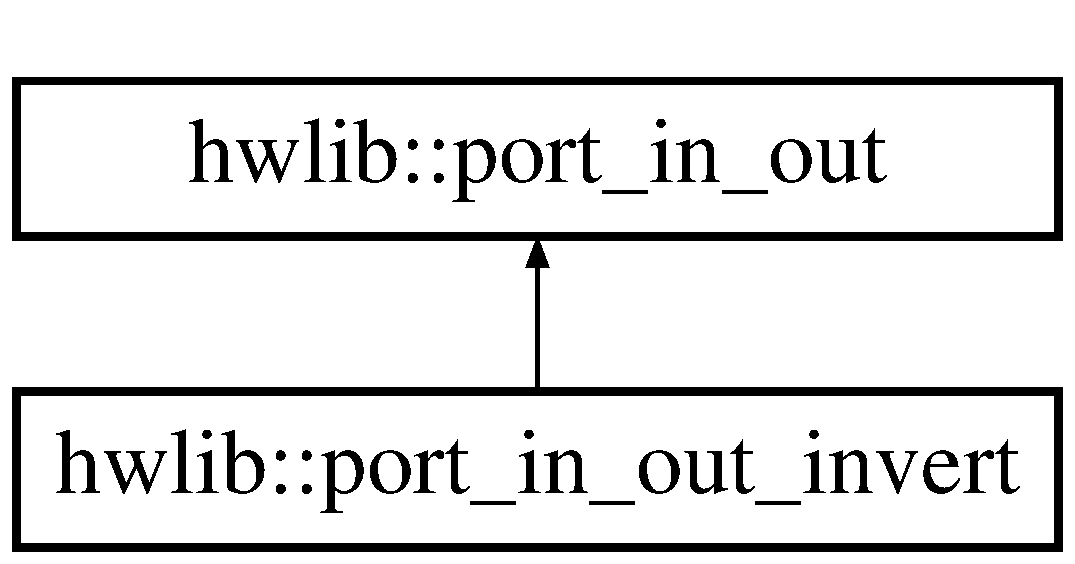
\includegraphics[height=2.000000cm]{classhwlib_1_1port__in__out__invert}
\end{center}
\end{figure}
\subsection*{Public Member Functions}
\begin{DoxyCompactItemize}
\item 
\hyperlink{classhwlib_1_1port__in__out__invert_a973654f691225df539a0d1340c205722}{port\+\_\+in\+\_\+out\+\_\+invert} (\hyperlink{classhwlib_1_1port__in__out}{port\+\_\+in\+\_\+out} \&port)
\begin{DoxyCompactList}\small\item\em construct an inverted input/output port \end{DoxyCompactList}\item 
void \hyperlink{classhwlib_1_1port__in__out__invert_aa9a02e447e2d960e8013300e4a06a35a}{direction\+\_\+set\+\_\+input} () override
\begin{DoxyCompactList}\small\item\em set the direction of the port to input. \end{DoxyCompactList}\item 
void \hyperlink{classhwlib_1_1port__in__out__invert_a038aeaafb573ef871d3608d489977a17}{direction\+\_\+set\+\_\+output} () override
\begin{DoxyCompactList}\small\item\em set the direction of the port to output \end{DoxyCompactList}\item 
uint\+\_\+fast8\+\_\+t \hyperlink{classhwlib_1_1port__in__out__invert_a8f3facb156f79e209a2db42b168edd46}{number\+\_\+of\+\_\+pins} () override
\begin{DoxyCompactList}\small\item\em get number of pins \end{DoxyCompactList}\item 
uint\+\_\+fast8\+\_\+t \hyperlink{classhwlib_1_1port__in__out__invert_ae7fac086fb1203b68376ec77a38e6187}{get} () override
\begin{DoxyCompactList}\small\item\em read from the port \end{DoxyCompactList}\item 
void \hyperlink{classhwlib_1_1port__in__out__invert_ac2d24269e7fd164fa3d32c4ead0bc6c7}{set} (uint\+\_\+fast8\+\_\+t x) override
\begin{DoxyCompactList}\small\item\em write to the port \end{DoxyCompactList}\end{DoxyCompactItemize}


\subsection{Detailed Description}
invert an input/input port 

This decorator inverts the result of read and write operations on an input port\+:
\begin{DoxyItemize}
\item When a value would be returned by the original port, the inverted port returns the value with all bits inverted.
\item When a value is written to the inverted output port, the inverse of that value is written to the original port. 
\end{DoxyItemize}

\subsection{Constructor \& Destructor Documentation}
\index{hwlib\+::port\+\_\+in\+\_\+out\+\_\+invert@{hwlib\+::port\+\_\+in\+\_\+out\+\_\+invert}!port\+\_\+in\+\_\+out\+\_\+invert@{port\+\_\+in\+\_\+out\+\_\+invert}}
\index{port\+\_\+in\+\_\+out\+\_\+invert@{port\+\_\+in\+\_\+out\+\_\+invert}!hwlib\+::port\+\_\+in\+\_\+out\+\_\+invert@{hwlib\+::port\+\_\+in\+\_\+out\+\_\+invert}}
\subsubsection[{\texorpdfstring{port\+\_\+in\+\_\+out\+\_\+invert(port\+\_\+in\+\_\+out \&port)}{port_in_out_invert(port_in_out &port)}}]{\setlength{\rightskip}{0pt plus 5cm}hwlib\+::port\+\_\+in\+\_\+out\+\_\+invert\+::port\+\_\+in\+\_\+out\+\_\+invert (
\begin{DoxyParamCaption}
\item[{{\bf port\+\_\+in\+\_\+out} \&}]{port}
\end{DoxyParamCaption}
)\hspace{0.3cm}{\ttfamily [inline]}}\hypertarget{classhwlib_1_1port__in__out__invert_a973654f691225df539a0d1340c205722}{}\label{classhwlib_1_1port__in__out__invert_a973654f691225df539a0d1340c205722}


construct an inverted input/output port 

This constructor creates an inverted input/output port from an existing input/output port. 

\subsection{Member Function Documentation}
\index{hwlib\+::port\+\_\+in\+\_\+out\+\_\+invert@{hwlib\+::port\+\_\+in\+\_\+out\+\_\+invert}!direction\+\_\+set\+\_\+input@{direction\+\_\+set\+\_\+input}}
\index{direction\+\_\+set\+\_\+input@{direction\+\_\+set\+\_\+input}!hwlib\+::port\+\_\+in\+\_\+out\+\_\+invert@{hwlib\+::port\+\_\+in\+\_\+out\+\_\+invert}}
\subsubsection[{\texorpdfstring{direction\+\_\+set\+\_\+input() override}{direction_set_input() override}}]{\setlength{\rightskip}{0pt plus 5cm}void hwlib\+::port\+\_\+in\+\_\+out\+\_\+invert\+::direction\+\_\+set\+\_\+input (
\begin{DoxyParamCaption}
{}
\end{DoxyParamCaption}
)\hspace{0.3cm}{\ttfamily [inline]}, {\ttfamily [override]}, {\ttfamily [virtual]}}\hypertarget{classhwlib_1_1port__in__out__invert_aa9a02e447e2d960e8013300e4a06a35a}{}\label{classhwlib_1_1port__in__out__invert_aa9a02e447e2d960e8013300e4a06a35a}


set the direction of the port to input. 

Calling this function sets all pins of the port to input. 

Implements \hyperlink{classhwlib_1_1port__in__out_ac7a9611410ddb9fd5d8e2dd15bff0a3f}{hwlib\+::port\+\_\+in\+\_\+out}.

\index{hwlib\+::port\+\_\+in\+\_\+out\+\_\+invert@{hwlib\+::port\+\_\+in\+\_\+out\+\_\+invert}!direction\+\_\+set\+\_\+output@{direction\+\_\+set\+\_\+output}}
\index{direction\+\_\+set\+\_\+output@{direction\+\_\+set\+\_\+output}!hwlib\+::port\+\_\+in\+\_\+out\+\_\+invert@{hwlib\+::port\+\_\+in\+\_\+out\+\_\+invert}}
\subsubsection[{\texorpdfstring{direction\+\_\+set\+\_\+output() override}{direction_set_output() override}}]{\setlength{\rightskip}{0pt plus 5cm}void hwlib\+::port\+\_\+in\+\_\+out\+\_\+invert\+::direction\+\_\+set\+\_\+output (
\begin{DoxyParamCaption}
{}
\end{DoxyParamCaption}
)\hspace{0.3cm}{\ttfamily [inline]}, {\ttfamily [override]}, {\ttfamily [virtual]}}\hypertarget{classhwlib_1_1port__in__out__invert_a038aeaafb573ef871d3608d489977a17}{}\label{classhwlib_1_1port__in__out__invert_a038aeaafb573ef871d3608d489977a17}


set the direction of the port to output 

Calling this function sets all pins of the port to output. 

Implements \hyperlink{classhwlib_1_1port__in__out_a515b4a6bbde4f2df5bb11cda41234fe4}{hwlib\+::port\+\_\+in\+\_\+out}.

\index{hwlib\+::port\+\_\+in\+\_\+out\+\_\+invert@{hwlib\+::port\+\_\+in\+\_\+out\+\_\+invert}!get@{get}}
\index{get@{get}!hwlib\+::port\+\_\+in\+\_\+out\+\_\+invert@{hwlib\+::port\+\_\+in\+\_\+out\+\_\+invert}}
\subsubsection[{\texorpdfstring{get() override}{get() override}}]{\setlength{\rightskip}{0pt plus 5cm}uint\+\_\+fast8\+\_\+t hwlib\+::port\+\_\+in\+\_\+out\+\_\+invert\+::get (
\begin{DoxyParamCaption}
{}
\end{DoxyParamCaption}
)\hspace{0.3cm}{\ttfamily [inline]}, {\ttfamily [override]}, {\ttfamily [virtual]}}\hypertarget{classhwlib_1_1port__in__out__invert_ae7fac086fb1203b68376ec77a38e6187}{}\label{classhwlib_1_1port__in__out__invert_ae7fac086fb1203b68376ec77a38e6187}


read from the port 

This function reads and returns the pins that are part of the port. The lowest bit of the result reflects the first pin of the port, etc.

Before calling this function the port direction must have been set to input by calling port\+\_\+direction\+\_\+set\+\_\+input(). 

Implements \hyperlink{classhwlib_1_1port__in__out_a822b44b3dd5b9df225e793896aeba641}{hwlib\+::port\+\_\+in\+\_\+out}.

\index{hwlib\+::port\+\_\+in\+\_\+out\+\_\+invert@{hwlib\+::port\+\_\+in\+\_\+out\+\_\+invert}!number\+\_\+of\+\_\+pins@{number\+\_\+of\+\_\+pins}}
\index{number\+\_\+of\+\_\+pins@{number\+\_\+of\+\_\+pins}!hwlib\+::port\+\_\+in\+\_\+out\+\_\+invert@{hwlib\+::port\+\_\+in\+\_\+out\+\_\+invert}}
\subsubsection[{\texorpdfstring{number\+\_\+of\+\_\+pins() override}{number_of_pins() override}}]{\setlength{\rightskip}{0pt plus 5cm}uint\+\_\+fast8\+\_\+t hwlib\+::port\+\_\+in\+\_\+out\+\_\+invert\+::number\+\_\+of\+\_\+pins (
\begin{DoxyParamCaption}
{}
\end{DoxyParamCaption}
)\hspace{0.3cm}{\ttfamily [inline]}, {\ttfamily [override]}, {\ttfamily [virtual]}}\hypertarget{classhwlib_1_1port__in__out__invert_a8f3facb156f79e209a2db42b168edd46}{}\label{classhwlib_1_1port__in__out__invert_a8f3facb156f79e209a2db42b168edd46}


get number of pins 

This function returns the number of pins in the port. 

Implements \hyperlink{classhwlib_1_1port__in__out_a44243a6c7664e734563f1809058751bc}{hwlib\+::port\+\_\+in\+\_\+out}.

\index{hwlib\+::port\+\_\+in\+\_\+out\+\_\+invert@{hwlib\+::port\+\_\+in\+\_\+out\+\_\+invert}!set@{set}}
\index{set@{set}!hwlib\+::port\+\_\+in\+\_\+out\+\_\+invert@{hwlib\+::port\+\_\+in\+\_\+out\+\_\+invert}}
\subsubsection[{\texorpdfstring{set(uint\+\_\+fast8\+\_\+t x) override}{set(uint_fast8_t x) override}}]{\setlength{\rightskip}{0pt plus 5cm}void hwlib\+::port\+\_\+in\+\_\+out\+\_\+invert\+::set (
\begin{DoxyParamCaption}
\item[{uint\+\_\+fast8\+\_\+t}]{x}
\end{DoxyParamCaption}
)\hspace{0.3cm}{\ttfamily [inline]}, {\ttfamily [override]}, {\ttfamily [virtual]}}\hypertarget{classhwlib_1_1port__in__out__invert_ac2d24269e7fd164fa3d32c4ead0bc6c7}{}\label{classhwlib_1_1port__in__out__invert_ac2d24269e7fd164fa3d32c4ead0bc6c7}


write to the port 

This function writes to the pins that are part of the port. The lowest bit is written to the first pin of the port, etc.

Before calling this function the port direction must have been set to output by calling \hyperlink{classhwlib_1_1port__in__out__invert_a038aeaafb573ef871d3608d489977a17}{direction\+\_\+set\+\_\+output()}. 

Implements \hyperlink{classhwlib_1_1port__in__out_adaca419a61193e42e06e52afbbc4afe4}{hwlib\+::port\+\_\+in\+\_\+out}.



The documentation for this class was generated from the following file\+:\begin{DoxyCompactItemize}
\item 
\hyperlink{hwlib-port_8hpp}{hwlib-\/port.\+hpp}\end{DoxyCompactItemize}

\hypertarget{classhwlib_1_1port__oc}{}\section{hwlib\+:\+:port\+\_\+oc Class Reference}
\label{classhwlib_1_1port__oc}\index{hwlib\+::port\+\_\+oc@{hwlib\+::port\+\_\+oc}}


open-\/collector interface  




{\ttfamily \#include $<$hwlib-\/port.\+hpp$>$}

Inheritance diagram for hwlib\+:\+:port\+\_\+oc\+:\begin{figure}[H]
\begin{center}
\leavevmode
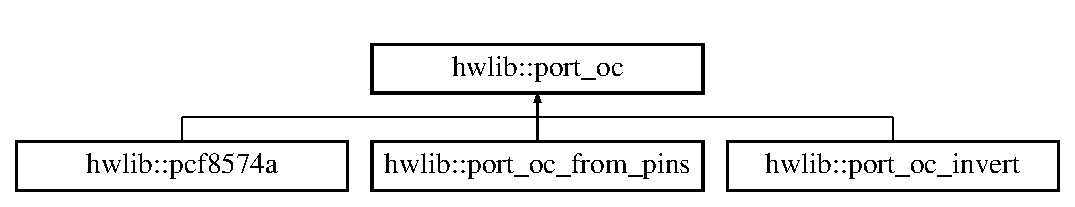
\includegraphics[height=2.000000cm]{classhwlib_1_1port__oc}
\end{center}
\end{figure}
\subsection*{Public Member Functions}
\begin{DoxyCompactItemize}
\item 
virtual uint\+\_\+fast8\+\_\+t \hyperlink{classhwlib_1_1port__oc_a44d0dbfde290ad17237ad70c09a4c402}{number\+\_\+of\+\_\+pins} ()=0
\begin{DoxyCompactList}\small\item\em get number of pins \end{DoxyCompactList}\item 
virtual uint\+\_\+fast8\+\_\+t \hyperlink{classhwlib_1_1port__oc_a49f8413dcdc6d9a172c2d9669a2e906e}{get} ()=0
\begin{DoxyCompactList}\small\item\em read from the port \end{DoxyCompactList}\item 
virtual void \hyperlink{classhwlib_1_1port__oc_aefb3d093331e5a87cf2dbe8226dc94ef}{set} (uint\+\_\+fast8\+\_\+t x)=0
\begin{DoxyCompactList}\small\item\em write to the port \end{DoxyCompactList}\end{DoxyCompactItemize}


\subsection{Detailed Description}
open-\/collector interface 

This is the interface of an open-\/collector port. 

\subsection{Member Function Documentation}
\index{hwlib\+::port\+\_\+oc@{hwlib\+::port\+\_\+oc}!get@{get}}
\index{get@{get}!hwlib\+::port\+\_\+oc@{hwlib\+::port\+\_\+oc}}
\subsubsection[{\texorpdfstring{get()=0}{get()=0}}]{\setlength{\rightskip}{0pt plus 5cm}virtual uint\+\_\+fast8\+\_\+t hwlib\+::port\+\_\+oc\+::get (
\begin{DoxyParamCaption}
{}
\end{DoxyParamCaption}
)\hspace{0.3cm}{\ttfamily [pure virtual]}}\hypertarget{classhwlib_1_1port__oc_a49f8413dcdc6d9a172c2d9669a2e906e}{}\label{classhwlib_1_1port__oc_a49f8413dcdc6d9a172c2d9669a2e906e}


read from the port 

This function reads and returns the pins that are part of the port. The lowest bit of the result reflects the first pin of the port, etc.

Pins that have been written as 0 will very likley read as 0 too. To read the external input to a pin, the pin must first be written as 1. 

Implemented in \hyperlink{classhwlib_1_1port__oc__invert_ab6d07c63e363949fd852b109b88923f7}{hwlib\+::port\+\_\+oc\+\_\+invert}, \hyperlink{classhwlib_1_1port__oc__from__pins_a89a18f8d370a872e1018275177be7649}{hwlib\+::port\+\_\+oc\+\_\+from\+\_\+pins}, and \hyperlink{classhwlib_1_1pcf8574a_abd2c5f791eced2e91f52db767351f0bd}{hwlib\+::pcf8574a}.

\index{hwlib\+::port\+\_\+oc@{hwlib\+::port\+\_\+oc}!number\+\_\+of\+\_\+pins@{number\+\_\+of\+\_\+pins}}
\index{number\+\_\+of\+\_\+pins@{number\+\_\+of\+\_\+pins}!hwlib\+::port\+\_\+oc@{hwlib\+::port\+\_\+oc}}
\subsubsection[{\texorpdfstring{number\+\_\+of\+\_\+pins()=0}{number_of_pins()=0}}]{\setlength{\rightskip}{0pt plus 5cm}virtual uint\+\_\+fast8\+\_\+t hwlib\+::port\+\_\+oc\+::number\+\_\+of\+\_\+pins (
\begin{DoxyParamCaption}
{}
\end{DoxyParamCaption}
)\hspace{0.3cm}{\ttfamily [pure virtual]}}\hypertarget{classhwlib_1_1port__oc_a44d0dbfde290ad17237ad70c09a4c402}{}\label{classhwlib_1_1port__oc_a44d0dbfde290ad17237ad70c09a4c402}


get number of pins 

This function returns the number of pins in the port. 

Implemented in \hyperlink{classhwlib_1_1port__oc__invert_a4dc1f8dec0b8a0b443523f29b1f78d65}{hwlib\+::port\+\_\+oc\+\_\+invert}, \hyperlink{classhwlib_1_1port__oc__from__pins_af5b1708778a9fca66d0d46b5a56797ef}{hwlib\+::port\+\_\+oc\+\_\+from\+\_\+pins}, and \hyperlink{classhwlib_1_1pcf8574a_a1bb2266c127d93fd1d7c0b3f9193817d}{hwlib\+::pcf8574a}.

\index{hwlib\+::port\+\_\+oc@{hwlib\+::port\+\_\+oc}!set@{set}}
\index{set@{set}!hwlib\+::port\+\_\+oc@{hwlib\+::port\+\_\+oc}}
\subsubsection[{\texorpdfstring{set(uint\+\_\+fast8\+\_\+t x)=0}{set(uint_fast8_t x)=0}}]{\setlength{\rightskip}{0pt plus 5cm}virtual void hwlib\+::port\+\_\+oc\+::set (
\begin{DoxyParamCaption}
\item[{uint\+\_\+fast8\+\_\+t}]{x}
\end{DoxyParamCaption}
)\hspace{0.3cm}{\ttfamily [pure virtual]}}\hypertarget{classhwlib_1_1port__oc_aefb3d093331e5a87cf2dbe8226dc94ef}{}\label{classhwlib_1_1port__oc_aefb3d093331e5a87cf2dbe8226dc94ef}


write to the port 

This function writes to the pins that are part of the port. The lowest bit is written to the first pin of the port, etc. 

Implemented in \hyperlink{classhwlib_1_1port__oc__invert_a1a3a108756e4de47025d6a065c91ff18}{hwlib\+::port\+\_\+oc\+\_\+invert}, \hyperlink{classhwlib_1_1port__oc__from__pins_a8f1a2fecaf1f5d8433ea4fc8d07a5efb}{hwlib\+::port\+\_\+oc\+\_\+from\+\_\+pins}, and \hyperlink{classhwlib_1_1pcf8574a_afeef7665cd9059959588295418c57709}{hwlib\+::pcf8574a}.



The documentation for this class was generated from the following file\+:\begin{DoxyCompactItemize}
\item 
\hyperlink{hwlib-port_8hpp}{hwlib-\/port.\+hpp}\end{DoxyCompactItemize}

\hypertarget{classhwlib_1_1port__oc__from__pins}{}\section{hwlib\+:\+:port\+\_\+oc\+\_\+from\+\_\+pins Class Reference}
\label{classhwlib_1_1port__oc__from__pins}\index{hwlib\+::port\+\_\+oc\+\_\+from\+\_\+pins@{hwlib\+::port\+\_\+oc\+\_\+from\+\_\+pins}}


opne\+\_\+collector port from open\+\_\+collector pins  




{\ttfamily \#include $<$hwlib-\/port.\+hpp$>$}

Inheritance diagram for hwlib\+:\+:port\+\_\+oc\+\_\+from\+\_\+pins\+:\begin{figure}[H]
\begin{center}
\leavevmode
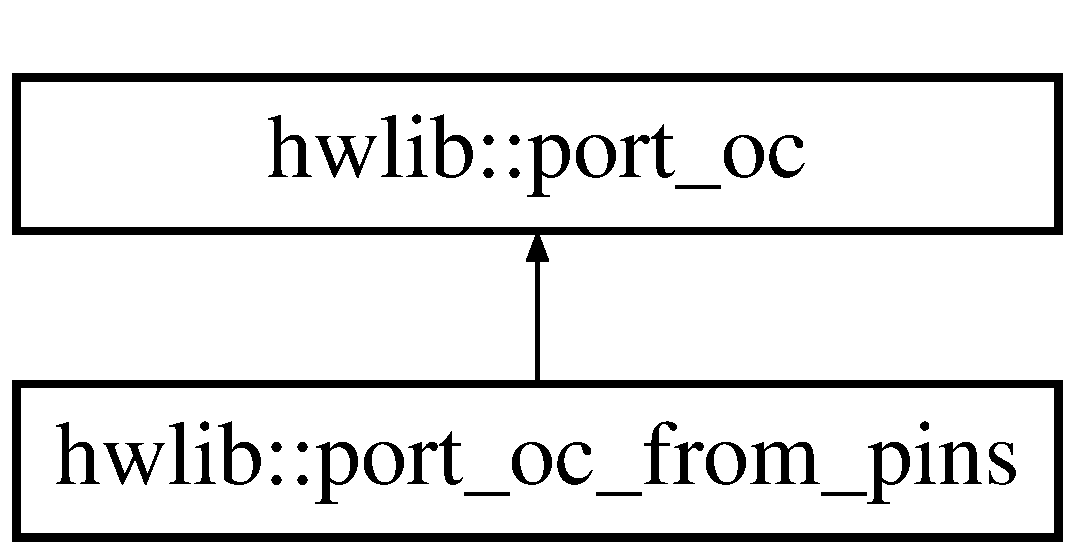
\includegraphics[height=2.000000cm]{classhwlib_1_1port__oc__from__pins}
\end{center}
\end{figure}
\subsection*{Public Member Functions}
\begin{DoxyCompactItemize}
\item 
\hyperlink{classhwlib_1_1port__oc__from__pins_a39e109f1ef3098baa00de94c34d90703}{port\+\_\+oc\+\_\+from\+\_\+pins} (\hyperlink{classhwlib_1_1pin__oc}{pin\+\_\+oc} \&p0=pin\+\_\+oc\+\_\+dummy, \hyperlink{classhwlib_1_1pin__oc}{pin\+\_\+oc} \&p1=pin\+\_\+oc\+\_\+dummy, \hyperlink{classhwlib_1_1pin__oc}{pin\+\_\+oc} \&p2=pin\+\_\+oc\+\_\+dummy, \hyperlink{classhwlib_1_1pin__oc}{pin\+\_\+oc} \&p3=pin\+\_\+oc\+\_\+dummy, \hyperlink{classhwlib_1_1pin__oc}{pin\+\_\+oc} \&p4=pin\+\_\+oc\+\_\+dummy, \hyperlink{classhwlib_1_1pin__oc}{pin\+\_\+oc} \&p5=pin\+\_\+oc\+\_\+dummy, \hyperlink{classhwlib_1_1pin__oc}{pin\+\_\+oc} \&p6=pin\+\_\+oc\+\_\+dummy, \hyperlink{classhwlib_1_1pin__oc}{pin\+\_\+oc} \&p7=pin\+\_\+oc\+\_\+dummy)
\begin{DoxyCompactList}\small\item\em construct a \hyperlink{classhwlib_1_1port__oc}{port\+\_\+oc} from up to 8 \hyperlink{classhwlib_1_1pin__oc}{pin\+\_\+oc} \end{DoxyCompactList}\item 
uint\+\_\+fast8\+\_\+t \hyperlink{classhwlib_1_1port__oc__from__pins_af5b1708778a9fca66d0d46b5a56797ef}{number\+\_\+of\+\_\+pins} () override
\begin{DoxyCompactList}\small\item\em get number of pins \end{DoxyCompactList}\item 
uint\+\_\+fast8\+\_\+t \hyperlink{classhwlib_1_1port__oc__from__pins_a89a18f8d370a872e1018275177be7649}{get} () override
\begin{DoxyCompactList}\small\item\em read from the port \end{DoxyCompactList}\item 
void \hyperlink{classhwlib_1_1port__oc__from__pins_a8f1a2fecaf1f5d8433ea4fc8d07a5efb}{set} (uint\+\_\+fast8\+\_\+t x) override
\begin{DoxyCompactList}\small\item\em write to the port \end{DoxyCompactList}\end{DoxyCompactItemize}


\subsection{Detailed Description}
opne\+\_\+collector port from open\+\_\+collector pins 

This class implements an open\+\_\+collector port made from port up to 8 pins. 

\subsection{Constructor \& Destructor Documentation}
\index{hwlib\+::port\+\_\+oc\+\_\+from\+\_\+pins@{hwlib\+::port\+\_\+oc\+\_\+from\+\_\+pins}!port\+\_\+oc\+\_\+from\+\_\+pins@{port\+\_\+oc\+\_\+from\+\_\+pins}}
\index{port\+\_\+oc\+\_\+from\+\_\+pins@{port\+\_\+oc\+\_\+from\+\_\+pins}!hwlib\+::port\+\_\+oc\+\_\+from\+\_\+pins@{hwlib\+::port\+\_\+oc\+\_\+from\+\_\+pins}}
\subsubsection[{\texorpdfstring{port\+\_\+oc\+\_\+from\+\_\+pins(pin\+\_\+oc \&p0=pin\+\_\+oc\+\_\+dummy, pin\+\_\+oc \&p1=pin\+\_\+oc\+\_\+dummy, pin\+\_\+oc \&p2=pin\+\_\+oc\+\_\+dummy, pin\+\_\+oc \&p3=pin\+\_\+oc\+\_\+dummy, pin\+\_\+oc \&p4=pin\+\_\+oc\+\_\+dummy, pin\+\_\+oc \&p5=pin\+\_\+oc\+\_\+dummy, pin\+\_\+oc \&p6=pin\+\_\+oc\+\_\+dummy, pin\+\_\+oc \&p7=pin\+\_\+oc\+\_\+dummy)}{port_oc_from_pins(pin_oc &p0=pin_oc_dummy, pin_oc &p1=pin_oc_dummy, pin_oc &p2=pin_oc_dummy, pin_oc &p3=pin_oc_dummy, pin_oc &p4=pin_oc_dummy, pin_oc &p5=pin_oc_dummy, pin_oc &p6=pin_oc_dummy, pin_oc &p7=pin_oc_dummy)}}]{\setlength{\rightskip}{0pt plus 5cm}hwlib\+::port\+\_\+oc\+\_\+from\+\_\+pins\+::port\+\_\+oc\+\_\+from\+\_\+pins (
\begin{DoxyParamCaption}
\item[{{\bf pin\+\_\+oc} \&}]{p0 = {\ttfamily pin\+\_\+oc\+\_\+dummy}, }
\item[{{\bf pin\+\_\+oc} \&}]{p1 = {\ttfamily pin\+\_\+oc\+\_\+dummy}, }
\item[{{\bf pin\+\_\+oc} \&}]{p2 = {\ttfamily pin\+\_\+oc\+\_\+dummy}, }
\item[{{\bf pin\+\_\+oc} \&}]{p3 = {\ttfamily pin\+\_\+oc\+\_\+dummy}, }
\item[{{\bf pin\+\_\+oc} \&}]{p4 = {\ttfamily pin\+\_\+oc\+\_\+dummy}, }
\item[{{\bf pin\+\_\+oc} \&}]{p5 = {\ttfamily pin\+\_\+oc\+\_\+dummy}, }
\item[{{\bf pin\+\_\+oc} \&}]{p6 = {\ttfamily pin\+\_\+oc\+\_\+dummy}, }
\item[{{\bf pin\+\_\+oc} \&}]{p7 = {\ttfamily pin\+\_\+oc\+\_\+dummy}}
\end{DoxyParamCaption}
)\hspace{0.3cm}{\ttfamily [inline]}}\hypertarget{classhwlib_1_1port__oc__from__pins_a39e109f1ef3098baa00de94c34d90703}{}\label{classhwlib_1_1port__oc__from__pins_a39e109f1ef3098baa00de94c34d90703}


construct a \hyperlink{classhwlib_1_1port__oc}{port\+\_\+oc} from up to 8 \hyperlink{classhwlib_1_1pin__oc}{pin\+\_\+oc} 

This constructor creates a \hyperlink{classhwlib_1_1port__oc}{port\+\_\+oc} from up to 8 \hyperlink{classhwlib_1_1pin__oc}{pin\+\_\+oc} pins. The first pin is the lowest pin in the port, etc. 

\subsection{Member Function Documentation}
\index{hwlib\+::port\+\_\+oc\+\_\+from\+\_\+pins@{hwlib\+::port\+\_\+oc\+\_\+from\+\_\+pins}!get@{get}}
\index{get@{get}!hwlib\+::port\+\_\+oc\+\_\+from\+\_\+pins@{hwlib\+::port\+\_\+oc\+\_\+from\+\_\+pins}}
\subsubsection[{\texorpdfstring{get() override}{get() override}}]{\setlength{\rightskip}{0pt plus 5cm}uint\+\_\+fast8\+\_\+t hwlib\+::port\+\_\+oc\+\_\+from\+\_\+pins\+::get (
\begin{DoxyParamCaption}
{}
\end{DoxyParamCaption}
)\hspace{0.3cm}{\ttfamily [inline]}, {\ttfamily [override]}, {\ttfamily [virtual]}}\hypertarget{classhwlib_1_1port__oc__from__pins_a89a18f8d370a872e1018275177be7649}{}\label{classhwlib_1_1port__oc__from__pins_a89a18f8d370a872e1018275177be7649}


read from the port 

This function reads and returns the pins that are part of the port. The lowest bit of the result reflects the first pin of the port, etc.

Pins that have been written as 0 will very likley read as 0 too. To read the external input to a pin, the pin must first be written as 1. 

Implements \hyperlink{classhwlib_1_1port__oc_a49f8413dcdc6d9a172c2d9669a2e906e}{hwlib\+::port\+\_\+oc}.

\index{hwlib\+::port\+\_\+oc\+\_\+from\+\_\+pins@{hwlib\+::port\+\_\+oc\+\_\+from\+\_\+pins}!number\+\_\+of\+\_\+pins@{number\+\_\+of\+\_\+pins}}
\index{number\+\_\+of\+\_\+pins@{number\+\_\+of\+\_\+pins}!hwlib\+::port\+\_\+oc\+\_\+from\+\_\+pins@{hwlib\+::port\+\_\+oc\+\_\+from\+\_\+pins}}
\subsubsection[{\texorpdfstring{number\+\_\+of\+\_\+pins() override}{number_of_pins() override}}]{\setlength{\rightskip}{0pt plus 5cm}uint\+\_\+fast8\+\_\+t hwlib\+::port\+\_\+oc\+\_\+from\+\_\+pins\+::number\+\_\+of\+\_\+pins (
\begin{DoxyParamCaption}
{}
\end{DoxyParamCaption}
)\hspace{0.3cm}{\ttfamily [inline]}, {\ttfamily [override]}, {\ttfamily [virtual]}}\hypertarget{classhwlib_1_1port__oc__from__pins_af5b1708778a9fca66d0d46b5a56797ef}{}\label{classhwlib_1_1port__oc__from__pins_af5b1708778a9fca66d0d46b5a56797ef}


get number of pins 

This function returns the number of pins in the port. 

Implements \hyperlink{classhwlib_1_1port__oc_a44d0dbfde290ad17237ad70c09a4c402}{hwlib\+::port\+\_\+oc}.

\index{hwlib\+::port\+\_\+oc\+\_\+from\+\_\+pins@{hwlib\+::port\+\_\+oc\+\_\+from\+\_\+pins}!set@{set}}
\index{set@{set}!hwlib\+::port\+\_\+oc\+\_\+from\+\_\+pins@{hwlib\+::port\+\_\+oc\+\_\+from\+\_\+pins}}
\subsubsection[{\texorpdfstring{set(uint\+\_\+fast8\+\_\+t x) override}{set(uint_fast8_t x) override}}]{\setlength{\rightskip}{0pt plus 5cm}void hwlib\+::port\+\_\+oc\+\_\+from\+\_\+pins\+::set (
\begin{DoxyParamCaption}
\item[{uint\+\_\+fast8\+\_\+t}]{x}
\end{DoxyParamCaption}
)\hspace{0.3cm}{\ttfamily [inline]}, {\ttfamily [override]}, {\ttfamily [virtual]}}\hypertarget{classhwlib_1_1port__oc__from__pins_a8f1a2fecaf1f5d8433ea4fc8d07a5efb}{}\label{classhwlib_1_1port__oc__from__pins_a8f1a2fecaf1f5d8433ea4fc8d07a5efb}


write to the port 

This function writes to the pins that are part of the port. The lowest bit is written to the first pin of the port, etc. 

Implements \hyperlink{classhwlib_1_1port__oc_aefb3d093331e5a87cf2dbe8226dc94ef}{hwlib\+::port\+\_\+oc}.



The documentation for this class was generated from the following file\+:\begin{DoxyCompactItemize}
\item 
\hyperlink{hwlib-port_8hpp}{hwlib-\/port.\+hpp}\end{DoxyCompactItemize}

\hypertarget{classhwlib_1_1port__oc__invert}{}\section{hwlib\+:\+:port\+\_\+oc\+\_\+invert Class Reference}
\label{classhwlib_1_1port__oc__invert}\index{hwlib\+::port\+\_\+oc\+\_\+invert@{hwlib\+::port\+\_\+oc\+\_\+invert}}


invert an open-\/collector port  




{\ttfamily \#include $<$hwlib-\/port.\+hpp$>$}

Inheritance diagram for hwlib\+:\+:port\+\_\+oc\+\_\+invert\+:\begin{figure}[H]
\begin{center}
\leavevmode
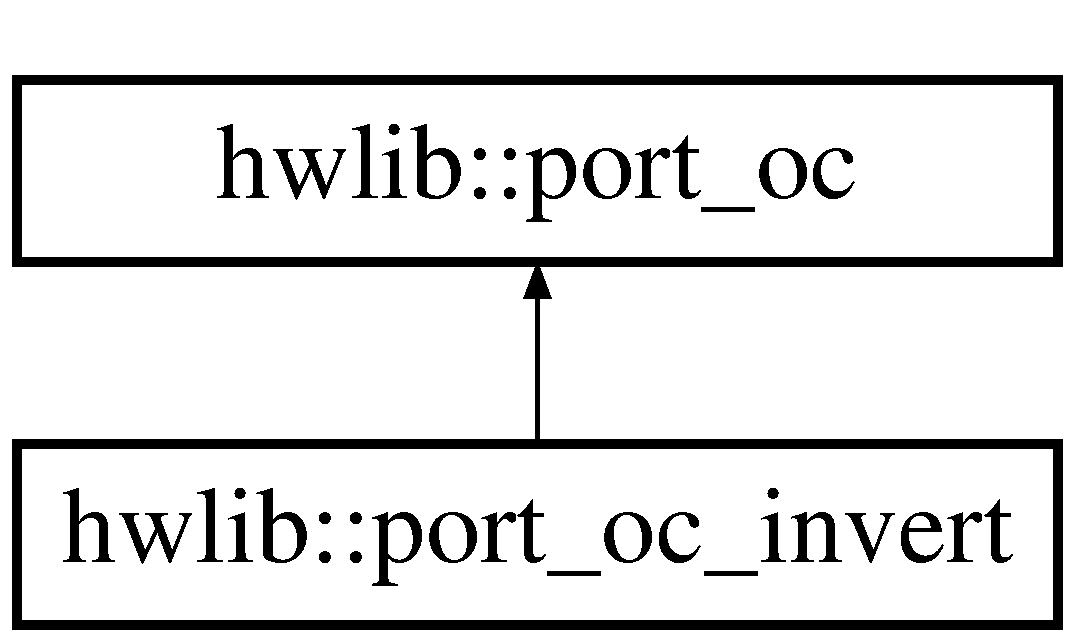
\includegraphics[height=2.000000cm]{classhwlib_1_1port__oc__invert}
\end{center}
\end{figure}
\subsection*{Public Member Functions}
\begin{DoxyCompactItemize}
\item 
\hyperlink{classhwlib_1_1port__oc__invert_ac475bce6da1c77573122a4bc23ee7997}{port\+\_\+oc\+\_\+invert} (\hyperlink{classhwlib_1_1port__oc}{port\+\_\+oc} \&port)
\begin{DoxyCompactList}\small\item\em construct an inverted open-\/collector port \end{DoxyCompactList}\item 
uint\+\_\+fast8\+\_\+t \hyperlink{classhwlib_1_1port__oc__invert_a4dc1f8dec0b8a0b443523f29b1f78d65}{number\+\_\+of\+\_\+pins} () override
\begin{DoxyCompactList}\small\item\em get number of pins \end{DoxyCompactList}\item 
uint\+\_\+fast8\+\_\+t \hyperlink{classhwlib_1_1port__oc__invert_ab6d07c63e363949fd852b109b88923f7}{get} () override
\begin{DoxyCompactList}\small\item\em read from the port \end{DoxyCompactList}\item 
void \hyperlink{classhwlib_1_1port__oc__invert_a1a3a108756e4de47025d6a065c91ff18}{set} (uint\+\_\+fast8\+\_\+t x) override
\begin{DoxyCompactList}\small\item\em write to the port \end{DoxyCompactList}\end{DoxyCompactItemize}


\subsection{Detailed Description}
invert an open-\/collector port 

This decorator inverts the result of read and write operations on an input port\+:
\begin{DoxyItemize}
\item When a value would be returned by the original port, the inverted port returns the value with all bits inverted.
\item When a value is written to the inverted output port, the inverse of that value is written to the original port. 
\end{DoxyItemize}

\subsection{Constructor \& Destructor Documentation}
\index{hwlib\+::port\+\_\+oc\+\_\+invert@{hwlib\+::port\+\_\+oc\+\_\+invert}!port\+\_\+oc\+\_\+invert@{port\+\_\+oc\+\_\+invert}}
\index{port\+\_\+oc\+\_\+invert@{port\+\_\+oc\+\_\+invert}!hwlib\+::port\+\_\+oc\+\_\+invert@{hwlib\+::port\+\_\+oc\+\_\+invert}}
\subsubsection[{\texorpdfstring{port\+\_\+oc\+\_\+invert(port\+\_\+oc \&port)}{port_oc_invert(port_oc &port)}}]{\setlength{\rightskip}{0pt plus 5cm}hwlib\+::port\+\_\+oc\+\_\+invert\+::port\+\_\+oc\+\_\+invert (
\begin{DoxyParamCaption}
\item[{{\bf port\+\_\+oc} \&}]{port}
\end{DoxyParamCaption}
)\hspace{0.3cm}{\ttfamily [inline]}}\hypertarget{classhwlib_1_1port__oc__invert_ac475bce6da1c77573122a4bc23ee7997}{}\label{classhwlib_1_1port__oc__invert_ac475bce6da1c77573122a4bc23ee7997}


construct an inverted open-\/collector port 

This constructor creates an inverted open-\/collector port from an existing open-\/collector port. 

\subsection{Member Function Documentation}
\index{hwlib\+::port\+\_\+oc\+\_\+invert@{hwlib\+::port\+\_\+oc\+\_\+invert}!get@{get}}
\index{get@{get}!hwlib\+::port\+\_\+oc\+\_\+invert@{hwlib\+::port\+\_\+oc\+\_\+invert}}
\subsubsection[{\texorpdfstring{get() override}{get() override}}]{\setlength{\rightskip}{0pt plus 5cm}uint\+\_\+fast8\+\_\+t hwlib\+::port\+\_\+oc\+\_\+invert\+::get (
\begin{DoxyParamCaption}
{}
\end{DoxyParamCaption}
)\hspace{0.3cm}{\ttfamily [inline]}, {\ttfamily [override]}, {\ttfamily [virtual]}}\hypertarget{classhwlib_1_1port__oc__invert_ab6d07c63e363949fd852b109b88923f7}{}\label{classhwlib_1_1port__oc__invert_ab6d07c63e363949fd852b109b88923f7}


read from the port 

This function reads and returns the pins that are part of the port. The lowest bit of the result reflects the first pin of the port, etc.

Pins that have been written as 0 will very likley read as 0 too. To read the external input to a pin, the pin must first be written as 1. 

Implements \hyperlink{classhwlib_1_1port__oc_a49f8413dcdc6d9a172c2d9669a2e906e}{hwlib\+::port\+\_\+oc}.

\index{hwlib\+::port\+\_\+oc\+\_\+invert@{hwlib\+::port\+\_\+oc\+\_\+invert}!number\+\_\+of\+\_\+pins@{number\+\_\+of\+\_\+pins}}
\index{number\+\_\+of\+\_\+pins@{number\+\_\+of\+\_\+pins}!hwlib\+::port\+\_\+oc\+\_\+invert@{hwlib\+::port\+\_\+oc\+\_\+invert}}
\subsubsection[{\texorpdfstring{number\+\_\+of\+\_\+pins() override}{number_of_pins() override}}]{\setlength{\rightskip}{0pt plus 5cm}uint\+\_\+fast8\+\_\+t hwlib\+::port\+\_\+oc\+\_\+invert\+::number\+\_\+of\+\_\+pins (
\begin{DoxyParamCaption}
{}
\end{DoxyParamCaption}
)\hspace{0.3cm}{\ttfamily [inline]}, {\ttfamily [override]}, {\ttfamily [virtual]}}\hypertarget{classhwlib_1_1port__oc__invert_a4dc1f8dec0b8a0b443523f29b1f78d65}{}\label{classhwlib_1_1port__oc__invert_a4dc1f8dec0b8a0b443523f29b1f78d65}


get number of pins 

This function returns the number of pins in the port. 

Implements \hyperlink{classhwlib_1_1port__oc_a44d0dbfde290ad17237ad70c09a4c402}{hwlib\+::port\+\_\+oc}.

\index{hwlib\+::port\+\_\+oc\+\_\+invert@{hwlib\+::port\+\_\+oc\+\_\+invert}!set@{set}}
\index{set@{set}!hwlib\+::port\+\_\+oc\+\_\+invert@{hwlib\+::port\+\_\+oc\+\_\+invert}}
\subsubsection[{\texorpdfstring{set(uint\+\_\+fast8\+\_\+t x) override}{set(uint_fast8_t x) override}}]{\setlength{\rightskip}{0pt plus 5cm}void hwlib\+::port\+\_\+oc\+\_\+invert\+::set (
\begin{DoxyParamCaption}
\item[{uint\+\_\+fast8\+\_\+t}]{x}
\end{DoxyParamCaption}
)\hspace{0.3cm}{\ttfamily [inline]}, {\ttfamily [override]}, {\ttfamily [virtual]}}\hypertarget{classhwlib_1_1port__oc__invert_a1a3a108756e4de47025d6a065c91ff18}{}\label{classhwlib_1_1port__oc__invert_a1a3a108756e4de47025d6a065c91ff18}


write to the port 

This function writes to the pins that are part of the port. The lowest bit is written to the first pin of the port, etc. 

Implements \hyperlink{classhwlib_1_1port__oc_aefb3d093331e5a87cf2dbe8226dc94ef}{hwlib\+::port\+\_\+oc}.



The documentation for this class was generated from the following file\+:\begin{DoxyCompactItemize}
\item 
\hyperlink{hwlib-port_8hpp}{hwlib-\/port.\+hpp}\end{DoxyCompactItemize}

\hypertarget{classhwlib_1_1port__out}{}\section{hwlib\+:\+:port\+\_\+out Class Reference}
\label{classhwlib_1_1port__out}\index{hwlib\+::port\+\_\+out@{hwlib\+::port\+\_\+out}}


output port interface  




{\ttfamily \#include $<$hwlib-\/port.\+hpp$>$}

Inheritance diagram for hwlib\+:\+:port\+\_\+out\+:\begin{figure}[H]
\begin{center}
\leavevmode
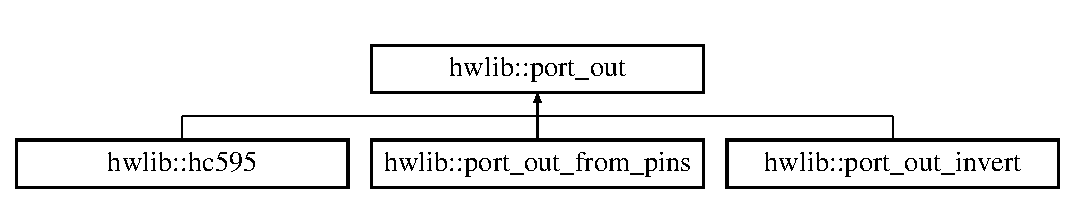
\includegraphics[height=2.000000cm]{classhwlib_1_1port__out}
\end{center}
\end{figure}
\subsection*{Public Member Functions}
\begin{DoxyCompactItemize}
\item 
virtual uint\+\_\+fast8\+\_\+t \hyperlink{classhwlib_1_1port__out_a8593e2ff755b938797defb06c1e085df}{number\+\_\+of\+\_\+pins} ()=0
\begin{DoxyCompactList}\small\item\em get number of pins \end{DoxyCompactList}\item 
virtual void \hyperlink{classhwlib_1_1port__out_ad086f5dd66f293118df6ab979feb64fc}{set} (uint\+\_\+fast8\+\_\+t x)=0
\begin{DoxyCompactList}\small\item\em write to the port \end{DoxyCompactList}\end{DoxyCompactItemize}


\subsection{Detailed Description}
output port interface 

This is the interface of an output-\/only port. 

\subsection{Member Function Documentation}
\index{hwlib\+::port\+\_\+out@{hwlib\+::port\+\_\+out}!number\+\_\+of\+\_\+pins@{number\+\_\+of\+\_\+pins}}
\index{number\+\_\+of\+\_\+pins@{number\+\_\+of\+\_\+pins}!hwlib\+::port\+\_\+out@{hwlib\+::port\+\_\+out}}
\subsubsection[{\texorpdfstring{number\+\_\+of\+\_\+pins()=0}{number_of_pins()=0}}]{\setlength{\rightskip}{0pt plus 5cm}virtual uint\+\_\+fast8\+\_\+t hwlib\+::port\+\_\+out\+::number\+\_\+of\+\_\+pins (
\begin{DoxyParamCaption}
{}
\end{DoxyParamCaption}
)\hspace{0.3cm}{\ttfamily [pure virtual]}}\hypertarget{classhwlib_1_1port__out_a8593e2ff755b938797defb06c1e085df}{}\label{classhwlib_1_1port__out_a8593e2ff755b938797defb06c1e085df}


get number of pins 

This function returns the number of pins in the port. 

Implemented in \hyperlink{classhwlib_1_1port__out__invert_aae7f6f49900f5e4108595a094f467cb8}{hwlib\+::port\+\_\+out\+\_\+invert}, \hyperlink{classhwlib_1_1hc595_a89c7b21cb99d61c91f764a0fdb7ceb9b}{hwlib\+::hc595}, and \hyperlink{classhwlib_1_1port__out__from__pins_afc18ca0fb161e581efcf88c65c0baebc}{hwlib\+::port\+\_\+out\+\_\+from\+\_\+pins}.

\index{hwlib\+::port\+\_\+out@{hwlib\+::port\+\_\+out}!set@{set}}
\index{set@{set}!hwlib\+::port\+\_\+out@{hwlib\+::port\+\_\+out}}
\subsubsection[{\texorpdfstring{set(uint\+\_\+fast8\+\_\+t x)=0}{set(uint_fast8_t x)=0}}]{\setlength{\rightskip}{0pt plus 5cm}virtual void hwlib\+::port\+\_\+out\+::set (
\begin{DoxyParamCaption}
\item[{uint\+\_\+fast8\+\_\+t}]{x}
\end{DoxyParamCaption}
)\hspace{0.3cm}{\ttfamily [pure virtual]}}\hypertarget{classhwlib_1_1port__out_ad086f5dd66f293118df6ab979feb64fc}{}\label{classhwlib_1_1port__out_ad086f5dd66f293118df6ab979feb64fc}


write to the port 

This function writes to the pins that are part of the port. The lowest bit is written to the first pin of the port, etc. 

Implemented in \hyperlink{classhwlib_1_1port__out__invert_a112ff1c0afec7813ce35830f20a3acb3}{hwlib\+::port\+\_\+out\+\_\+invert}, \hyperlink{classhwlib_1_1hc595_ad2b4d6fa77114f1f13348075389efd1c}{hwlib\+::hc595}, and \hyperlink{classhwlib_1_1port__out__from__pins_aefa5fd9f8d8756fb7c07a89eff03caa4}{hwlib\+::port\+\_\+out\+\_\+from\+\_\+pins}.



The documentation for this class was generated from the following file\+:\begin{DoxyCompactItemize}
\item 
\hyperlink{hwlib-port_8hpp}{hwlib-\/port.\+hpp}\end{DoxyCompactItemize}

\hypertarget{classhwlib_1_1port__out__from__pins}{}\section{hwlib\+:\+:port\+\_\+out\+\_\+from\+\_\+pins Class Reference}
\label{classhwlib_1_1port__out__from__pins}\index{hwlib\+::port\+\_\+out\+\_\+from\+\_\+pins@{hwlib\+::port\+\_\+out\+\_\+from\+\_\+pins}}


output port from output pins  




{\ttfamily \#include $<$hwlib-\/port.\+hpp$>$}

Inheritance diagram for hwlib\+:\+:port\+\_\+out\+\_\+from\+\_\+pins\+:\begin{figure}[H]
\begin{center}
\leavevmode
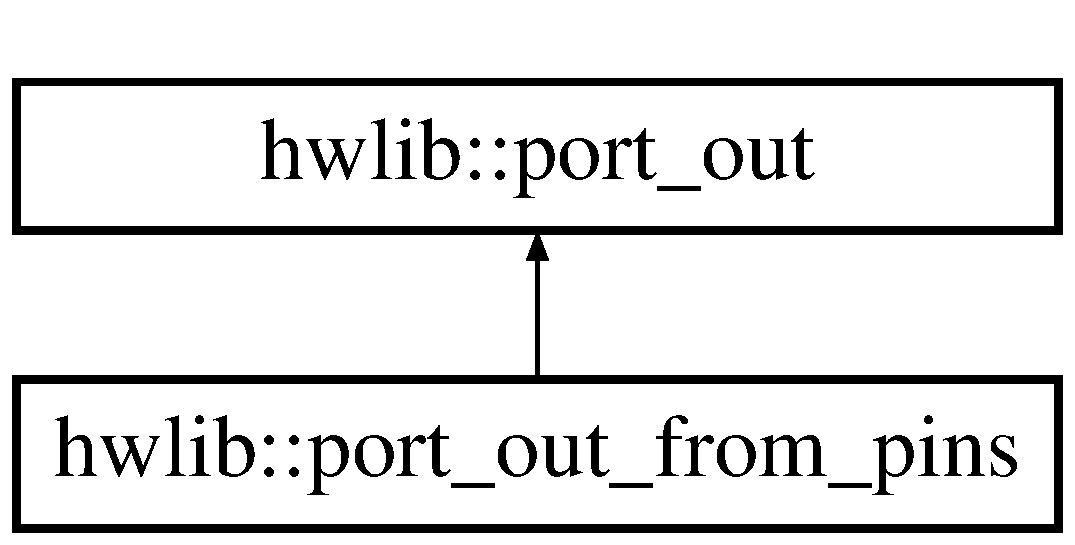
\includegraphics[height=2.000000cm]{classhwlib_1_1port__out__from__pins}
\end{center}
\end{figure}
\subsection*{Public Member Functions}
\begin{DoxyCompactItemize}
\item 
\hyperlink{classhwlib_1_1port__out__from__pins_af72ebaf01a3b43493d0cd60da2f66420}{port\+\_\+out\+\_\+from\+\_\+pins} (\hyperlink{classhwlib_1_1pin__out}{pin\+\_\+out} \&p0=pin\+\_\+out\+\_\+dummy, \hyperlink{classhwlib_1_1pin__out}{pin\+\_\+out} \&p1=pin\+\_\+out\+\_\+dummy, \hyperlink{classhwlib_1_1pin__out}{pin\+\_\+out} \&p2=pin\+\_\+out\+\_\+dummy, \hyperlink{classhwlib_1_1pin__out}{pin\+\_\+out} \&p3=pin\+\_\+out\+\_\+dummy, \hyperlink{classhwlib_1_1pin__out}{pin\+\_\+out} \&p4=pin\+\_\+out\+\_\+dummy, \hyperlink{classhwlib_1_1pin__out}{pin\+\_\+out} \&p5=pin\+\_\+out\+\_\+dummy, \hyperlink{classhwlib_1_1pin__out}{pin\+\_\+out} \&p6=pin\+\_\+out\+\_\+dummy, \hyperlink{classhwlib_1_1pin__out}{pin\+\_\+out} \&p7=pin\+\_\+out\+\_\+dummy)
\begin{DoxyCompactList}\small\item\em construct a \hyperlink{classhwlib_1_1port__out}{port\+\_\+out} from up to 8 pin\+\_\+outs \end{DoxyCompactList}\item 
uint\+\_\+fast8\+\_\+t \hyperlink{classhwlib_1_1port__out__from__pins_afc18ca0fb161e581efcf88c65c0baebc}{number\+\_\+of\+\_\+pins} () override
\begin{DoxyCompactList}\small\item\em get number of pins \end{DoxyCompactList}\item 
void \hyperlink{classhwlib_1_1port__out__from__pins_aefa5fd9f8d8756fb7c07a89eff03caa4}{set} (uint\+\_\+fast8\+\_\+t x) override
\begin{DoxyCompactList}\small\item\em write to the port \end{DoxyCompactList}\end{DoxyCompactItemize}


\subsection{Detailed Description}
output port from output pins 

This class implements an output-\/only port made from port up to 8 pins. 

\subsection{Constructor \& Destructor Documentation}
\index{hwlib\+::port\+\_\+out\+\_\+from\+\_\+pins@{hwlib\+::port\+\_\+out\+\_\+from\+\_\+pins}!port\+\_\+out\+\_\+from\+\_\+pins@{port\+\_\+out\+\_\+from\+\_\+pins}}
\index{port\+\_\+out\+\_\+from\+\_\+pins@{port\+\_\+out\+\_\+from\+\_\+pins}!hwlib\+::port\+\_\+out\+\_\+from\+\_\+pins@{hwlib\+::port\+\_\+out\+\_\+from\+\_\+pins}}
\subsubsection[{\texorpdfstring{port\+\_\+out\+\_\+from\+\_\+pins(pin\+\_\+out \&p0=pin\+\_\+out\+\_\+dummy, pin\+\_\+out \&p1=pin\+\_\+out\+\_\+dummy, pin\+\_\+out \&p2=pin\+\_\+out\+\_\+dummy, pin\+\_\+out \&p3=pin\+\_\+out\+\_\+dummy, pin\+\_\+out \&p4=pin\+\_\+out\+\_\+dummy, pin\+\_\+out \&p5=pin\+\_\+out\+\_\+dummy, pin\+\_\+out \&p6=pin\+\_\+out\+\_\+dummy, pin\+\_\+out \&p7=pin\+\_\+out\+\_\+dummy)}{port_out_from_pins(pin_out &p0=pin_out_dummy, pin_out &p1=pin_out_dummy, pin_out &p2=pin_out_dummy, pin_out &p3=pin_out_dummy, pin_out &p4=pin_out_dummy, pin_out &p5=pin_out_dummy, pin_out &p6=pin_out_dummy, pin_out &p7=pin_out_dummy)}}]{\setlength{\rightskip}{0pt plus 5cm}hwlib\+::port\+\_\+out\+\_\+from\+\_\+pins\+::port\+\_\+out\+\_\+from\+\_\+pins (
\begin{DoxyParamCaption}
\item[{{\bf pin\+\_\+out} \&}]{p0 = {\ttfamily pin\+\_\+out\+\_\+dummy}, }
\item[{{\bf pin\+\_\+out} \&}]{p1 = {\ttfamily pin\+\_\+out\+\_\+dummy}, }
\item[{{\bf pin\+\_\+out} \&}]{p2 = {\ttfamily pin\+\_\+out\+\_\+dummy}, }
\item[{{\bf pin\+\_\+out} \&}]{p3 = {\ttfamily pin\+\_\+out\+\_\+dummy}, }
\item[{{\bf pin\+\_\+out} \&}]{p4 = {\ttfamily pin\+\_\+out\+\_\+dummy}, }
\item[{{\bf pin\+\_\+out} \&}]{p5 = {\ttfamily pin\+\_\+out\+\_\+dummy}, }
\item[{{\bf pin\+\_\+out} \&}]{p6 = {\ttfamily pin\+\_\+out\+\_\+dummy}, }
\item[{{\bf pin\+\_\+out} \&}]{p7 = {\ttfamily pin\+\_\+out\+\_\+dummy}}
\end{DoxyParamCaption}
)\hspace{0.3cm}{\ttfamily [inline]}}\hypertarget{classhwlib_1_1port__out__from__pins_af72ebaf01a3b43493d0cd60da2f66420}{}\label{classhwlib_1_1port__out__from__pins_af72ebaf01a3b43493d0cd60da2f66420}


construct a \hyperlink{classhwlib_1_1port__out}{port\+\_\+out} from up to 8 pin\+\_\+outs 

This constructor creates a \hyperlink{classhwlib_1_1port__out}{port\+\_\+out} from up to 8 \hyperlink{classhwlib_1_1pin__out}{pin\+\_\+out} pins. The first pin is the lowest pin in the port, etc. 

\subsection{Member Function Documentation}
\index{hwlib\+::port\+\_\+out\+\_\+from\+\_\+pins@{hwlib\+::port\+\_\+out\+\_\+from\+\_\+pins}!number\+\_\+of\+\_\+pins@{number\+\_\+of\+\_\+pins}}
\index{number\+\_\+of\+\_\+pins@{number\+\_\+of\+\_\+pins}!hwlib\+::port\+\_\+out\+\_\+from\+\_\+pins@{hwlib\+::port\+\_\+out\+\_\+from\+\_\+pins}}
\subsubsection[{\texorpdfstring{number\+\_\+of\+\_\+pins() override}{number_of_pins() override}}]{\setlength{\rightskip}{0pt plus 5cm}uint\+\_\+fast8\+\_\+t hwlib\+::port\+\_\+out\+\_\+from\+\_\+pins\+::number\+\_\+of\+\_\+pins (
\begin{DoxyParamCaption}
{}
\end{DoxyParamCaption}
)\hspace{0.3cm}{\ttfamily [inline]}, {\ttfamily [override]}, {\ttfamily [virtual]}}\hypertarget{classhwlib_1_1port__out__from__pins_afc18ca0fb161e581efcf88c65c0baebc}{}\label{classhwlib_1_1port__out__from__pins_afc18ca0fb161e581efcf88c65c0baebc}


get number of pins 

This function returns the number of pins in the port. 

Implements \hyperlink{classhwlib_1_1port__out_a8593e2ff755b938797defb06c1e085df}{hwlib\+::port\+\_\+out}.

\index{hwlib\+::port\+\_\+out\+\_\+from\+\_\+pins@{hwlib\+::port\+\_\+out\+\_\+from\+\_\+pins}!set@{set}}
\index{set@{set}!hwlib\+::port\+\_\+out\+\_\+from\+\_\+pins@{hwlib\+::port\+\_\+out\+\_\+from\+\_\+pins}}
\subsubsection[{\texorpdfstring{set(uint\+\_\+fast8\+\_\+t x) override}{set(uint_fast8_t x) override}}]{\setlength{\rightskip}{0pt plus 5cm}void hwlib\+::port\+\_\+out\+\_\+from\+\_\+pins\+::set (
\begin{DoxyParamCaption}
\item[{uint\+\_\+fast8\+\_\+t}]{x}
\end{DoxyParamCaption}
)\hspace{0.3cm}{\ttfamily [inline]}, {\ttfamily [override]}, {\ttfamily [virtual]}}\hypertarget{classhwlib_1_1port__out__from__pins_aefa5fd9f8d8756fb7c07a89eff03caa4}{}\label{classhwlib_1_1port__out__from__pins_aefa5fd9f8d8756fb7c07a89eff03caa4}


write to the port 

This function writes to the pins that are part of the port. The lowest bit is written to the first pin of the port, etc. 

Implements \hyperlink{classhwlib_1_1port__out_ad086f5dd66f293118df6ab979feb64fc}{hwlib\+::port\+\_\+out}.



The documentation for this class was generated from the following file\+:\begin{DoxyCompactItemize}
\item 
\hyperlink{hwlib-port_8hpp}{hwlib-\/port.\+hpp}\end{DoxyCompactItemize}

\hypertarget{classhwlib_1_1port__out__invert}{}\section{hwlib\+:\+:port\+\_\+out\+\_\+invert Class Reference}
\label{classhwlib_1_1port__out__invert}\index{hwlib\+::port\+\_\+out\+\_\+invert@{hwlib\+::port\+\_\+out\+\_\+invert}}


invert an output port  




{\ttfamily \#include $<$hwlib-\/port.\+hpp$>$}

Inheritance diagram for hwlib\+:\+:port\+\_\+out\+\_\+invert\+:\begin{figure}[H]
\begin{center}
\leavevmode
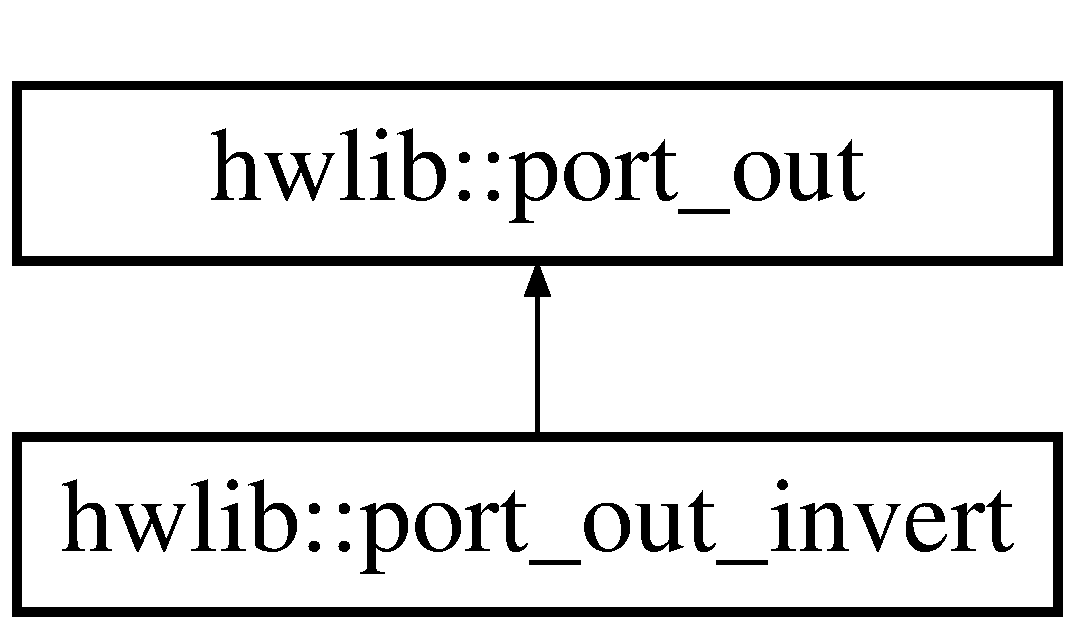
\includegraphics[height=2.000000cm]{classhwlib_1_1port__out__invert}
\end{center}
\end{figure}
\subsection*{Public Member Functions}
\begin{DoxyCompactItemize}
\item 
\hyperlink{classhwlib_1_1port__out__invert_a4939b1992b6142487c0c537c7a6d29b6}{port\+\_\+out\+\_\+invert} (\hyperlink{classhwlib_1_1port__out}{port\+\_\+out} \&port)
\begin{DoxyCompactList}\small\item\em construct an inverted output port \end{DoxyCompactList}\item 
uint\+\_\+fast8\+\_\+t \hyperlink{classhwlib_1_1port__out__invert_aae7f6f49900f5e4108595a094f467cb8}{number\+\_\+of\+\_\+pins} () override
\begin{DoxyCompactList}\small\item\em get number of pins \end{DoxyCompactList}\item 
void \hyperlink{classhwlib_1_1port__out__invert_a112ff1c0afec7813ce35830f20a3acb3}{set} (uint\+\_\+fast8\+\_\+t x) override
\begin{DoxyCompactList}\small\item\em write to the port \end{DoxyCompactList}\end{DoxyCompactItemize}


\subsection{Detailed Description}
invert an output port 

This decorator inverts the effect of write operations to an output port\+: When a value is written to this inverted output port, the inverse of that value is written to the original port. 

\subsection{Constructor \& Destructor Documentation}
\index{hwlib\+::port\+\_\+out\+\_\+invert@{hwlib\+::port\+\_\+out\+\_\+invert}!port\+\_\+out\+\_\+invert@{port\+\_\+out\+\_\+invert}}
\index{port\+\_\+out\+\_\+invert@{port\+\_\+out\+\_\+invert}!hwlib\+::port\+\_\+out\+\_\+invert@{hwlib\+::port\+\_\+out\+\_\+invert}}
\subsubsection[{\texorpdfstring{port\+\_\+out\+\_\+invert(port\+\_\+out \&port)}{port_out_invert(port_out &port)}}]{\setlength{\rightskip}{0pt plus 5cm}hwlib\+::port\+\_\+out\+\_\+invert\+::port\+\_\+out\+\_\+invert (
\begin{DoxyParamCaption}
\item[{{\bf port\+\_\+out} \&}]{port}
\end{DoxyParamCaption}
)\hspace{0.3cm}{\ttfamily [inline]}}\hypertarget{classhwlib_1_1port__out__invert_a4939b1992b6142487c0c537c7a6d29b6}{}\label{classhwlib_1_1port__out__invert_a4939b1992b6142487c0c537c7a6d29b6}


construct an inverted output port 

This constructor creates an inverted output port from an existing output port. 

\subsection{Member Function Documentation}
\index{hwlib\+::port\+\_\+out\+\_\+invert@{hwlib\+::port\+\_\+out\+\_\+invert}!number\+\_\+of\+\_\+pins@{number\+\_\+of\+\_\+pins}}
\index{number\+\_\+of\+\_\+pins@{number\+\_\+of\+\_\+pins}!hwlib\+::port\+\_\+out\+\_\+invert@{hwlib\+::port\+\_\+out\+\_\+invert}}
\subsubsection[{\texorpdfstring{number\+\_\+of\+\_\+pins() override}{number_of_pins() override}}]{\setlength{\rightskip}{0pt plus 5cm}uint\+\_\+fast8\+\_\+t hwlib\+::port\+\_\+out\+\_\+invert\+::number\+\_\+of\+\_\+pins (
\begin{DoxyParamCaption}
{}
\end{DoxyParamCaption}
)\hspace{0.3cm}{\ttfamily [inline]}, {\ttfamily [override]}, {\ttfamily [virtual]}}\hypertarget{classhwlib_1_1port__out__invert_aae7f6f49900f5e4108595a094f467cb8}{}\label{classhwlib_1_1port__out__invert_aae7f6f49900f5e4108595a094f467cb8}


get number of pins 

This function returns the number of pins in the port. 

Implements \hyperlink{classhwlib_1_1port__out_a8593e2ff755b938797defb06c1e085df}{hwlib\+::port\+\_\+out}.

\index{hwlib\+::port\+\_\+out\+\_\+invert@{hwlib\+::port\+\_\+out\+\_\+invert}!set@{set}}
\index{set@{set}!hwlib\+::port\+\_\+out\+\_\+invert@{hwlib\+::port\+\_\+out\+\_\+invert}}
\subsubsection[{\texorpdfstring{set(uint\+\_\+fast8\+\_\+t x) override}{set(uint_fast8_t x) override}}]{\setlength{\rightskip}{0pt plus 5cm}void hwlib\+::port\+\_\+out\+\_\+invert\+::set (
\begin{DoxyParamCaption}
\item[{uint\+\_\+fast8\+\_\+t}]{x}
\end{DoxyParamCaption}
)\hspace{0.3cm}{\ttfamily [inline]}, {\ttfamily [override]}, {\ttfamily [virtual]}}\hypertarget{classhwlib_1_1port__out__invert_a112ff1c0afec7813ce35830f20a3acb3}{}\label{classhwlib_1_1port__out__invert_a112ff1c0afec7813ce35830f20a3acb3}


write to the port 

This function writes to the pins that are part of the port. The lowest bit is written to the first pin of the port, etc. 

Implements \hyperlink{classhwlib_1_1port__out_ad086f5dd66f293118df6ab979feb64fc}{hwlib\+::port\+\_\+out}.



The documentation for this class was generated from the following file\+:\begin{DoxyCompactItemize}
\item 
\hyperlink{hwlib-port_8hpp}{hwlib-\/port.\+hpp}\end{DoxyCompactItemize}

\hypertarget{structsam3xa}{}\section{sam3xa Struct Reference}
\label{structsam3xa}\index{sam3xa@{sam3xa}}
\subsection*{Static Public Member Functions}
\begin{DoxyCompactItemize}
\item 
static void \hyperlink{structsam3xa_a5c64fdd7a44e7283a371095eb5006822}{System\+Init} (void)\hypertarget{structsam3xa_a5c64fdd7a44e7283a371095eb5006822}{}\label{structsam3xa_a5c64fdd7a44e7283a371095eb5006822}

\begin{DoxyCompactList}\small\item\em Setup the microcontroller system. Initialize the System and update the System\+Frequency variable. \end{DoxyCompactList}\item 
static void {\bfseries System\+Core\+Clock\+Update} (void)\hypertarget{structsam3xa_a706dfb7f27503c306abec713add9fe01}{}\label{structsam3xa_a706dfb7f27503c306abec713add9fe01}

\item 
static void \hyperlink{structsam3xa_a2145370cebb05a883057a5591ab69b47}{system\+\_\+init\+\_\+flash} (uint32\+\_\+t dw\+\_\+clk)
\end{DoxyCompactItemize}
\subsection*{Static Public Attributes}
\begin{DoxyCompactItemize}
\item 
static uint32\+\_\+t {\bfseries System\+Core\+Clock} = C\+H\+I\+P\+\_\+\+F\+R\+E\+Q\+\_\+\+M\+A\+I\+N\+C\+K\+\_\+\+R\+C\+\_\+4\+M\+HZ\hypertarget{structsam3xa_abe7d91288a97f62ac2101fbfa0d6e3cc}{}\label{structsam3xa_abe7d91288a97f62ac2101fbfa0d6e3cc}

\end{DoxyCompactItemize}


\subsection{Member Function Documentation}
\index{sam3xa@{sam3xa}!system\+\_\+init\+\_\+flash@{system\+\_\+init\+\_\+flash}}
\index{system\+\_\+init\+\_\+flash@{system\+\_\+init\+\_\+flash}!sam3xa@{sam3xa}}
\subsubsection[{\texorpdfstring{system\+\_\+init\+\_\+flash(uint32\+\_\+t dw\+\_\+clk)}{system_init_flash(uint32_t dw_clk)}}]{\setlength{\rightskip}{0pt plus 5cm}static void sam3xa\+::system\+\_\+init\+\_\+flash (
\begin{DoxyParamCaption}
\item[{uint32\+\_\+t}]{dw\+\_\+clk}
\end{DoxyParamCaption}
)\hspace{0.3cm}{\ttfamily [inline]}, {\ttfamily [static]}}\hypertarget{structsam3xa_a2145370cebb05a883057a5591ab69b47}{}\label{structsam3xa_a2145370cebb05a883057a5591ab69b47}
Initialize flash. 

The documentation for this struct was generated from the following file\+:\begin{DoxyCompactItemize}
\item 
hwlib-\/due-\/system-\/sam3xa.\+hpp\end{DoxyCompactItemize}

\hypertarget{structhwlib_1_1setfill}{}\section{hwlib\+:\+:setfill Struct Reference}
\label{structhwlib_1_1setfill}\index{hwlib\+::setfill@{hwlib\+::setfill}}


ostream filler character manipulator  




{\ttfamily \#include $<$hwlib-\/ostream -\/ Copy.\+hpp$>$}

\subsection*{Public Member Functions}
\begin{DoxyCompactItemize}
\item 
constexpr \hyperlink{structhwlib_1_1setfill_a42ba50078ab62623475986d0f7ab4545}{setfill} (char x)
\begin{DoxyCompactList}\small\item\em ostream filler character manipulator \end{DoxyCompactList}\item 
constexpr \hyperlink{structhwlib_1_1setfill_a42ba50078ab62623475986d0f7ab4545}{setfill} (char x)
\begin{DoxyCompactList}\small\item\em ostream filler character manipulator \end{DoxyCompactList}\end{DoxyCompactItemize}


\subsection{Detailed Description}
ostream filler character manipulator 

\subsection{Constructor \& Destructor Documentation}
\index{hwlib\+::setfill@{hwlib\+::setfill}!setfill@{setfill}}
\index{setfill@{setfill}!hwlib\+::setfill@{hwlib\+::setfill}}
\subsubsection[{\texorpdfstring{setfill(char x)}{setfill(char x)}}]{\setlength{\rightskip}{0pt plus 5cm}constexpr hwlib\+::setfill\+::setfill (
\begin{DoxyParamCaption}
\item[{char}]{x}
\end{DoxyParamCaption}
)\hspace{0.3cm}{\ttfamily [inline]}}\hypertarget{structhwlib_1_1setfill_a42ba50078ab62623475986d0f7ab4545}{}\label{structhwlib_1_1setfill_a42ba50078ab62623475986d0f7ab4545}


ostream filler character manipulator 

Writing setfill(\+C) to an ostream sets filler character that is used to pad an item when it is smaller than the current field width.

The same effect can be achieved by calling stream.\+setfill(\+C). \index{hwlib\+::setfill@{hwlib\+::setfill}!setfill@{setfill}}
\index{setfill@{setfill}!hwlib\+::setfill@{hwlib\+::setfill}}
\subsubsection[{\texorpdfstring{setfill(char x)}{setfill(char x)}}]{\setlength{\rightskip}{0pt plus 5cm}constexpr hwlib\+::setfill\+::setfill (
\begin{DoxyParamCaption}
\item[{char}]{x}
\end{DoxyParamCaption}
)\hspace{0.3cm}{\ttfamily [inline]}}\hypertarget{structhwlib_1_1setfill_a42ba50078ab62623475986d0f7ab4545}{}\label{structhwlib_1_1setfill_a42ba50078ab62623475986d0f7ab4545}


ostream filler character manipulator 

Writing setfill(\+C) to an ostream sets filler character that is used to pad an item when it is smaller than the current field width.

The same effect can be achieved by calling stream.\+setfill(\+C). 

The documentation for this struct was generated from the following files\+:\begin{DoxyCompactItemize}
\item 
\hyperlink{hwlib-ostream_01-_01_copy_8hpp}{hwlib-\/ostream -\/ Copy.\+hpp}\item 
\hyperlink{hwlib-ostream_8hpp}{hwlib-\/ostream.\+hpp}\end{DoxyCompactItemize}

\hypertarget{structhwlib_1_1setw}{}\section{hwlib\+:\+:setw Struct Reference}
\label{structhwlib_1_1setw}\index{hwlib\+::setw@{hwlib\+::setw}}


ostream output field width manipulator  




{\ttfamily \#include $<$hwlib-\/ostream -\/ Copy.\+hpp$>$}

\subsection*{Public Member Functions}
\begin{DoxyCompactItemize}
\item 
constexpr \hyperlink{structhwlib_1_1setw_a673323de9e3a3caa26818d2b2f7eed6e}{setw} (int x)
\begin{DoxyCompactList}\small\item\em ostream output field width manipulator \end{DoxyCompactList}\item 
constexpr \hyperlink{structhwlib_1_1setw_a673323de9e3a3caa26818d2b2f7eed6e}{setw} (int x)
\begin{DoxyCompactList}\small\item\em ostream output field width manipulator \end{DoxyCompactList}\end{DoxyCompactItemize}


\subsection{Detailed Description}
ostream output field width manipulator 

\subsection{Constructor \& Destructor Documentation}
\index{hwlib\+::setw@{hwlib\+::setw}!setw@{setw}}
\index{setw@{setw}!hwlib\+::setw@{hwlib\+::setw}}
\subsubsection[{\texorpdfstring{setw(int x)}{setw(int x)}}]{\setlength{\rightskip}{0pt plus 5cm}constexpr hwlib\+::setw\+::setw (
\begin{DoxyParamCaption}
\item[{int}]{x}
\end{DoxyParamCaption}
)\hspace{0.3cm}{\ttfamily [inline]}}\hypertarget{structhwlib_1_1setw_a673323de9e3a3caa26818d2b2f7eed6e}{}\label{structhwlib_1_1setw_a673323de9e3a3caa26818d2b2f7eed6e}


ostream output field width manipulator 

Writing the setw(\+N) manipulator to an ostream sets the minimum width of the field in which the next item is written to N\+: If the item is smaller than N, it will be padded with fill characters.

Setting the field width has an effect only on the next item that is printed, after that the field width resets to its initial value of 0.

The same effect can be achieved by calling stream.\+setw(\+N). \index{hwlib\+::setw@{hwlib\+::setw}!setw@{setw}}
\index{setw@{setw}!hwlib\+::setw@{hwlib\+::setw}}
\subsubsection[{\texorpdfstring{setw(int x)}{setw(int x)}}]{\setlength{\rightskip}{0pt plus 5cm}constexpr hwlib\+::setw\+::setw (
\begin{DoxyParamCaption}
\item[{int}]{x}
\end{DoxyParamCaption}
)\hspace{0.3cm}{\ttfamily [inline]}}\hypertarget{structhwlib_1_1setw_a673323de9e3a3caa26818d2b2f7eed6e}{}\label{structhwlib_1_1setw_a673323de9e3a3caa26818d2b2f7eed6e}


ostream output field width manipulator 

Writing the setw(\+N) manipulator to an ostream sets the minimum width of the field in which the next item is written to N\+: If the item is smaller than N, it will be padded with fill characters.

Setting the field width has an effect only on the next item that is printed, after that the field width resets to its initial value of 0.

The same effect can be achieved by calling stream.\+setw(\+N). 

The documentation for this struct was generated from the following files\+:\begin{DoxyCompactItemize}
\item 
\hyperlink{hwlib-ostream_01-_01_copy_8hpp}{hwlib-\/ostream -\/ Copy.\+hpp}\item 
\hyperlink{hwlib-ostream_8hpp}{hwlib-\/ostream.\+hpp}\end{DoxyCompactItemize}

\hypertarget{classhwlib_1_1spi__bus}{}\section{hwlib\+:\+:spi\+\_\+bus Class Reference}
\label{classhwlib_1_1spi__bus}\index{hwlib\+::spi\+\_\+bus@{hwlib\+::spi\+\_\+bus}}


spi bus interface  




{\ttfamily \#include $<$hwlib-\/spi.\+hpp$>$}

Inheritance diagram for hwlib\+:\+:spi\+\_\+bus\+:\begin{figure}[H]
\begin{center}
\leavevmode
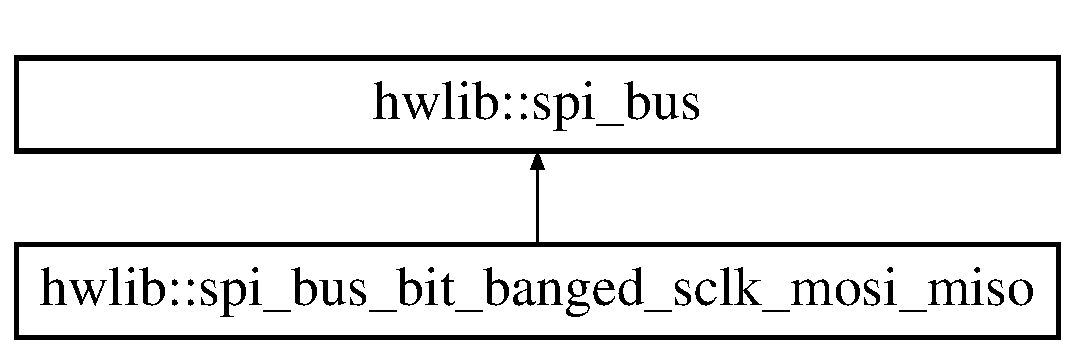
\includegraphics[height=2.000000cm]{classhwlib_1_1spi__bus}
\end{center}
\end{figure}
\subsection*{Public Member Functions}
\begin{DoxyCompactItemize}
\item 
virtual void \hyperlink{classhwlib_1_1spi__bus_ae6e20e12c547c64b6456997d938b6943}{write\+\_\+and\+\_\+read} (\hyperlink{classhwlib_1_1pin__out}{pin\+\_\+out} \&sel, int n, const \hyperlink{hwlib-defines_8hpp_ab8ef12fab634c171394422d0ee8baf94}{byte} data\+\_\+out\mbox{[}$\,$\mbox{]}, \hyperlink{hwlib-defines_8hpp_ab8ef12fab634c171394422d0ee8baf94}{byte} data\+\_\+in\mbox{[}$\,$\mbox{]})=0
\begin{DoxyCompactList}\small\item\em spi read-\/and-\/write transaction \end{DoxyCompactList}\end{DoxyCompactItemize}


\subsection{Detailed Description}
spi bus interface 

This class abstracts the interface of a master to a S\+PI bus.

The S\+PI (Serial Peripheral Interface) protocol is based on shift registers. The master (in most cases the micro-\/controller) generates clock pulses (S\+C\+LK), and on each pulse one bit of data is transferred from the shift register inside the master to the shift register inside the slave, A\+ND one bit is transferred in the other direction. After N clock pulses, all N data bits in the master and the slave are exchanged. The M\+O\+SI line transfers data from master to slave (Master Out Slave In), the M\+I\+SO (Master In Slave Out) line transfers data from the slave to the master.



The SS (Slave Select) line is used to signal the start and end of a S\+P\+OI transfer. In most cases, the select line is active low.



A S\+PI bus can have multiple slaves. All slaves (and the master) share the M\+O\+SI, M\+I\+SO and S\+L\+CK lines. Each slave has a separate SS line, that is used to activate a single slave for a transfer.



The S\+PI bus is a de-\/facto standard\+: there is no official document that defines it, but various manufacturers agree on how it should work and (more or less!) implement it the same. But there are differences that might give problems\+:
\begin{DoxyItemize}
\item the polarity (active low or active high) of the SS line
\item the initial level of the clock
\item the polarity of the clock (the clock edge on which the master and slave transfer data)
\item the (maximum) clock frequency
\end{DoxyItemize}

As always, consult the datasheet of the chip for the details.

references\+:
\begin{DoxyItemize}
\item \href{https://embeddedmicro.com/tutorials/mojo/serial-peripheral-interface-spi}{\tt S\+PI explanation} (Embedded Micro Forum)
\item \href{https://en.wikipedia.org/wiki/Serial_Peripheral_Interface_Bus}{\tt Serial Peripheral Bus} (wikipedia) 
\end{DoxyItemize}

\subsection{Member Function Documentation}
\index{hwlib\+::spi\+\_\+bus@{hwlib\+::spi\+\_\+bus}!write\+\_\+and\+\_\+read@{write\+\_\+and\+\_\+read}}
\index{write\+\_\+and\+\_\+read@{write\+\_\+and\+\_\+read}!hwlib\+::spi\+\_\+bus@{hwlib\+::spi\+\_\+bus}}
\subsubsection[{\texorpdfstring{write\+\_\+and\+\_\+read(pin\+\_\+out \&sel, int n, const byte data\+\_\+out[], byte data\+\_\+in[])=0}{write_and_read(pin_out &sel, int n, const byte data_out[], byte data_in[])=0}}]{\setlength{\rightskip}{0pt plus 5cm}virtual void hwlib\+::spi\+\_\+bus\+::write\+\_\+and\+\_\+read (
\begin{DoxyParamCaption}
\item[{{\bf pin\+\_\+out} \&}]{sel, }
\item[{int}]{n, }
\item[{const {\bf byte}}]{data\+\_\+out\mbox{[}$\,$\mbox{]}, }
\item[{{\bf byte}}]{data\+\_\+in\mbox{[}$\,$\mbox{]}}
\end{DoxyParamCaption}
)\hspace{0.3cm}{\ttfamily [pure virtual]}}\hypertarget{classhwlib_1_1spi__bus_ae6e20e12c547c64b6456997d938b6943}{}\label{classhwlib_1_1spi__bus_ae6e20e12c547c64b6456997d938b6943}


spi read-\/and-\/write transaction 

This function simultaneously writes n bytes from data\+\_\+out\mbox{[}\mbox{]} to the slave activated by the sel pin, and reads n bytes into data\+\_\+in\mbox{[}\mbox{]}. When data\+\_\+out is a nullptr, all-\/0 bytes are written. When data\+\_\+in is a nullptr, the data that is read is not stored. 

Implemented in \hyperlink{classhwlib_1_1spi__bus__bit__banged__sclk__mosi__miso_aa54c0f670505249860f59d8d62b982ca}{hwlib\+::spi\+\_\+bus\+\_\+bit\+\_\+banged\+\_\+sclk\+\_\+mosi\+\_\+miso}.



The documentation for this class was generated from the following file\+:\begin{DoxyCompactItemize}
\item 
\hyperlink{hwlib-spi_8hpp}{hwlib-\/spi.\+hpp}\end{DoxyCompactItemize}

\hypertarget{classhwlib_1_1spi__bus__bit__banged__sclk__mosi__miso}{}\section{hwlib\+:\+:spi\+\_\+bus\+\_\+bit\+\_\+banged\+\_\+sclk\+\_\+mosi\+\_\+miso Class Reference}
\label{classhwlib_1_1spi__bus__bit__banged__sclk__mosi__miso}\index{hwlib\+::spi\+\_\+bus\+\_\+bit\+\_\+banged\+\_\+sclk\+\_\+mosi\+\_\+miso@{hwlib\+::spi\+\_\+bus\+\_\+bit\+\_\+banged\+\_\+sclk\+\_\+mosi\+\_\+miso}}


bit-\/banged S\+PI bus implementation  




{\ttfamily \#include $<$hwlib-\/spi.\+hpp$>$}

Inheritance diagram for hwlib\+:\+:spi\+\_\+bus\+\_\+bit\+\_\+banged\+\_\+sclk\+\_\+mosi\+\_\+miso\+:\begin{figure}[H]
\begin{center}
\leavevmode
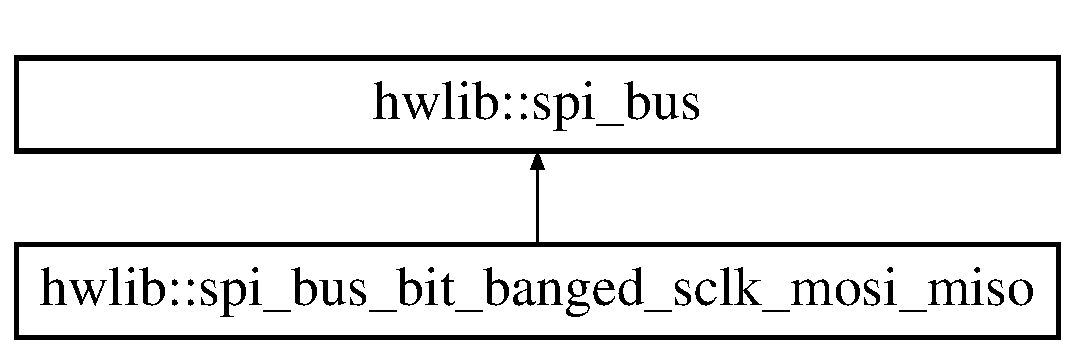
\includegraphics[height=2.000000cm]{classhwlib_1_1spi__bus__bit__banged__sclk__mosi__miso}
\end{center}
\end{figure}
\subsection*{Public Member Functions}
\begin{DoxyCompactItemize}
\item 
\hyperlink{classhwlib_1_1spi__bus__bit__banged__sclk__mosi__miso_aec1da306136cb0bb367dd47470f551da}{spi\+\_\+bus\+\_\+bit\+\_\+banged\+\_\+sclk\+\_\+mosi\+\_\+miso} (\hyperlink{classhwlib_1_1pin__out}{pin\+\_\+out} \&sclk, \hyperlink{classhwlib_1_1pin__out}{pin\+\_\+out} \&mosi, \hyperlink{classhwlib_1_1pin__in}{pin\+\_\+in} \&miso)
\begin{DoxyCompactList}\small\item\em construct a bit-\/banged S\+PI bus from the sclk, miso and mosi pins \end{DoxyCompactList}\item 
void \hyperlink{classhwlib_1_1spi__bus__bit__banged__sclk__mosi__miso_aa54c0f670505249860f59d8d62b982ca}{write\+\_\+and\+\_\+read} (\hyperlink{classhwlib_1_1pin__out}{pin\+\_\+out} \&sel, int n, const \hyperlink{hwlib-defines_8hpp_ab8ef12fab634c171394422d0ee8baf94}{byte} data\+\_\+out\mbox{[}$\,$\mbox{]}, \hyperlink{hwlib-defines_8hpp_ab8ef12fab634c171394422d0ee8baf94}{byte} data\+\_\+in\mbox{[}$\,$\mbox{]}) override
\begin{DoxyCompactList}\small\item\em write and read to (and from) a spi chip \end{DoxyCompactList}\end{DoxyCompactItemize}


\subsection{Detailed Description}
bit-\/banged S\+PI bus implementation 

This class implements a bit-\/banged master interface to a S\+PI bus. 

\subsection{Constructor \& Destructor Documentation}
\index{hwlib\+::spi\+\_\+bus\+\_\+bit\+\_\+banged\+\_\+sclk\+\_\+mosi\+\_\+miso@{hwlib\+::spi\+\_\+bus\+\_\+bit\+\_\+banged\+\_\+sclk\+\_\+mosi\+\_\+miso}!spi\+\_\+bus\+\_\+bit\+\_\+banged\+\_\+sclk\+\_\+mosi\+\_\+miso@{spi\+\_\+bus\+\_\+bit\+\_\+banged\+\_\+sclk\+\_\+mosi\+\_\+miso}}
\index{spi\+\_\+bus\+\_\+bit\+\_\+banged\+\_\+sclk\+\_\+mosi\+\_\+miso@{spi\+\_\+bus\+\_\+bit\+\_\+banged\+\_\+sclk\+\_\+mosi\+\_\+miso}!hwlib\+::spi\+\_\+bus\+\_\+bit\+\_\+banged\+\_\+sclk\+\_\+mosi\+\_\+miso@{hwlib\+::spi\+\_\+bus\+\_\+bit\+\_\+banged\+\_\+sclk\+\_\+mosi\+\_\+miso}}
\subsubsection[{\texorpdfstring{spi\+\_\+bus\+\_\+bit\+\_\+banged\+\_\+sclk\+\_\+mosi\+\_\+miso(pin\+\_\+out \&sclk, pin\+\_\+out \&mosi, pin\+\_\+in \&miso)}{spi_bus_bit_banged_sclk_mosi_miso(pin_out &sclk, pin_out &mosi, pin_in &miso)}}]{\setlength{\rightskip}{0pt plus 5cm}hwlib\+::spi\+\_\+bus\+\_\+bit\+\_\+banged\+\_\+sclk\+\_\+mosi\+\_\+miso\+::spi\+\_\+bus\+\_\+bit\+\_\+banged\+\_\+sclk\+\_\+mosi\+\_\+miso (
\begin{DoxyParamCaption}
\item[{{\bf pin\+\_\+out} \&}]{sclk, }
\item[{{\bf pin\+\_\+out} \&}]{mosi, }
\item[{{\bf pin\+\_\+in} \&}]{miso}
\end{DoxyParamCaption}
)\hspace{0.3cm}{\ttfamily [inline]}}\hypertarget{classhwlib_1_1spi__bus__bit__banged__sclk__mosi__miso_aec1da306136cb0bb367dd47470f551da}{}\label{classhwlib_1_1spi__bus__bit__banged__sclk__mosi__miso_aec1da306136cb0bb367dd47470f551da}


construct a bit-\/banged S\+PI bus from the sclk, miso and mosi pins 

This constructor creates a bit-\/banged S\+PI bus master from the sclk, miso and mosi pins.

The chip select pins for the individual chips supplied to the \hyperlink{classhwlib_1_1spi__bus__bit__banged__sclk__mosi__miso_aa54c0f670505249860f59d8d62b982ca}{write\+\_\+and\+\_\+read()} functions.

When the S\+PI bus is used for either only writing or only reading, the unused pin argument can be specified as pin\+\_\+out\+\_\+dummy or pin\+\_\+in\+\_\+dummy. 

\subsection{Member Function Documentation}
\index{hwlib\+::spi\+\_\+bus\+\_\+bit\+\_\+banged\+\_\+sclk\+\_\+mosi\+\_\+miso@{hwlib\+::spi\+\_\+bus\+\_\+bit\+\_\+banged\+\_\+sclk\+\_\+mosi\+\_\+miso}!write\+\_\+and\+\_\+read@{write\+\_\+and\+\_\+read}}
\index{write\+\_\+and\+\_\+read@{write\+\_\+and\+\_\+read}!hwlib\+::spi\+\_\+bus\+\_\+bit\+\_\+banged\+\_\+sclk\+\_\+mosi\+\_\+miso@{hwlib\+::spi\+\_\+bus\+\_\+bit\+\_\+banged\+\_\+sclk\+\_\+mosi\+\_\+miso}}
\subsubsection[{\texorpdfstring{write\+\_\+and\+\_\+read(pin\+\_\+out \&sel, int n, const byte data\+\_\+out[], byte data\+\_\+in[]) override}{write_and_read(pin_out &sel, int n, const byte data_out[], byte data_in[]) override}}]{\setlength{\rightskip}{0pt plus 5cm}void hwlib\+::spi\+\_\+bus\+\_\+bit\+\_\+banged\+\_\+sclk\+\_\+mosi\+\_\+miso\+::write\+\_\+and\+\_\+read (
\begin{DoxyParamCaption}
\item[{{\bf pin\+\_\+out} \&}]{sel, }
\item[{int}]{n, }
\item[{const {\bf byte}}]{data\+\_\+out\mbox{[}$\,$\mbox{]}, }
\item[{{\bf byte}}]{data\+\_\+in\mbox{[}$\,$\mbox{]}}
\end{DoxyParamCaption}
)\hspace{0.3cm}{\ttfamily [inline]}, {\ttfamily [override]}, {\ttfamily [virtual]}}\hypertarget{classhwlib_1_1spi__bus__bit__banged__sclk__mosi__miso_aa54c0f670505249860f59d8d62b982ca}{}\label{classhwlib_1_1spi__bus__bit__banged__sclk__mosi__miso_aa54c0f670505249860f59d8d62b982ca}


write and read to (and from) a spi chip 

This function performs an n byte write-\/and-\/read operation on the S\+PI chip activated by the (active low) sel pin.

When either writing or reading is not needed the corresponding argument can be a nullptr. 

Implements \hyperlink{classhwlib_1_1spi__bus_ae6e20e12c547c64b6456997d938b6943}{hwlib\+::spi\+\_\+bus}.



The documentation for this class was generated from the following file\+:\begin{DoxyCompactItemize}
\item 
\hyperlink{hwlib-spi_8hpp}{hwlib-\/spi.\+hpp}\end{DoxyCompactItemize}

\hypertarget{classhwlib_1_1window}{}\section{hwlib\+:\+:window Class Reference}
\label{classhwlib_1_1window}\index{hwlib\+::window@{hwlib\+::window}}


a graphics window  




{\ttfamily \#include $<$hwlib-\/graphics.\+hpp$>$}

Inheritance diagram for hwlib\+:\+:window\+:\begin{figure}[H]
\begin{center}
\leavevmode
\includegraphics[height=1.357576cm]{classhwlib_1_1window}
\end{center}
\end{figure}
\subsection*{Public Member Functions}
\begin{DoxyCompactItemize}
\item 
\hyperlink{classhwlib_1_1window_a5acfb1afba5adade79ae1576831128f1}{window} (\hyperlink{classhwlib_1_1location}{location} \hyperlink{classhwlib_1_1window_ad2ad5281c9c09d18010b19cb807d3eaa}{size}, \hyperlink{classhwlib_1_1color}{color} \hyperlink{classhwlib_1_1window_a812e3bf440309bf3280d34fa04eeb718}{foreground}, \hyperlink{classhwlib_1_1color}{color} \hyperlink{classhwlib_1_1window_a1ca47e79ec54ea8b2f38b41b42593d2d}{background})\hypertarget{classhwlib_1_1window_a5acfb1afba5adade79ae1576831128f1}{}\label{classhwlib_1_1window_a5acfb1afba5adade79ae1576831128f1}

\begin{DoxyCompactList}\small\item\em construct a window by specifying its size and foreground and background colors. \end{DoxyCompactList}\item 
void \hyperlink{classhwlib_1_1window_a65122042afeb55e41e5c03b5c8e26fff}{write} (\hyperlink{classhwlib_1_1location}{location} pos, \hyperlink{classhwlib_1_1color}{color} col)
\begin{DoxyCompactList}\small\item\em write a pixel \end{DoxyCompactList}\item 
void \hyperlink{classhwlib_1_1window_ac87b3f0e82ab260f95a68e76f827d03b}{write} (\hyperlink{classhwlib_1_1location}{location} pos, const \hyperlink{classhwlib_1_1image}{image} \&img)
\begin{DoxyCompactList}\small\item\em write a rectangle of pixels \end{DoxyCompactList}\item 
void {\bfseries write} (\hyperlink{classhwlib_1_1location}{location} pos)\hypertarget{classhwlib_1_1window_ac90b74315df62b9952ce2ee3af95825b}{}\label{classhwlib_1_1window_ac90b74315df62b9952ce2ee3af95825b}

\item 
virtual void \hyperlink{classhwlib_1_1window_a5e781163353ce26cb4dc5b2cbe40ad05}{clear} ()
\begin{DoxyCompactList}\small\item\em clear the window \end{DoxyCompactList}\end{DoxyCompactItemize}
\subsection*{Public Attributes}
\begin{DoxyCompactItemize}
\item 
const \hyperlink{classhwlib_1_1location}{location} \hyperlink{classhwlib_1_1window_ad2ad5281c9c09d18010b19cb807d3eaa}{size}
\begin{DoxyCompactList}\small\item\em the size of the window \end{DoxyCompactList}\item 
\hyperlink{classhwlib_1_1color}{color} \hyperlink{classhwlib_1_1window_a812e3bf440309bf3280d34fa04eeb718}{foreground}
\begin{DoxyCompactList}\small\item\em the foreground color of the window \end{DoxyCompactList}\item 
\hyperlink{classhwlib_1_1color}{color} \hyperlink{classhwlib_1_1window_a1ca47e79ec54ea8b2f38b41b42593d2d}{background}
\begin{DoxyCompactList}\small\item\em the background color of the window \end{DoxyCompactList}\end{DoxyCompactItemize}


\subsection{Detailed Description}
a graphics window 

This class abstracts the interface to a graphic window. 

\subsection{Member Function Documentation}
\index{hwlib\+::window@{hwlib\+::window}!clear@{clear}}
\index{clear@{clear}!hwlib\+::window@{hwlib\+::window}}
\subsubsection[{\texorpdfstring{clear()}{clear()}}]{\setlength{\rightskip}{0pt plus 5cm}virtual void hwlib\+::window\+::clear (
\begin{DoxyParamCaption}
{}
\end{DoxyParamCaption}
)\hspace{0.3cm}{\ttfamily [inline]}, {\ttfamily [virtual]}}\hypertarget{classhwlib_1_1window_a5e781163353ce26cb4dc5b2cbe40ad05}{}\label{classhwlib_1_1window_a5e781163353ce26cb4dc5b2cbe40ad05}


clear the window 

This function clears the windows by writing the background color to all pixels. The default implementation writes to all pixels in sequence. A concrete window can probably provide a faster implementation. 

Reimplemented in \hyperlink{classhwlib_1_1glcd__oled__buffered_a1df3ca6d163e33b2edf1242acf47342a}{hwlib\+::glcd\+\_\+oled\+\_\+buffered}, \hyperlink{classhwlib_1_1glcd__oled_a4d3734f822d7f814be2630538cc49911}{hwlib\+::glcd\+\_\+oled}, and \hyperlink{classhwlib_1_1glcd__5510_a533b2663e151bee909543d0038b2cb4d}{hwlib\+::glcd\+\_\+5510}.

\index{hwlib\+::window@{hwlib\+::window}!write@{write}}
\index{write@{write}!hwlib\+::window@{hwlib\+::window}}
\subsubsection[{\texorpdfstring{write(location pos, color col)}{write(location pos, color col)}}]{\setlength{\rightskip}{0pt plus 5cm}void hwlib\+::window\+::write (
\begin{DoxyParamCaption}
\item[{{\bf location}}]{pos, }
\item[{{\bf color}}]{col}
\end{DoxyParamCaption}
)\hspace{0.3cm}{\ttfamily [inline]}}\hypertarget{classhwlib_1_1window_a65122042afeb55e41e5c03b5c8e26fff}{}\label{classhwlib_1_1window_a65122042afeb55e41e5c03b5c8e26fff}


write a pixel 

This function writes the color col to the pixel at location loc. If either the color is transparent, or the location is outside the window the call has no effect. When no locor is specificied, the window\textquotesingle{}s foreground color is used. \index{hwlib\+::window@{hwlib\+::window}!write@{write}}
\index{write@{write}!hwlib\+::window@{hwlib\+::window}}
\subsubsection[{\texorpdfstring{write(location pos, const image \&img)}{write(location pos, const image &img)}}]{\setlength{\rightskip}{0pt plus 5cm}void hwlib\+::window\+::write (
\begin{DoxyParamCaption}
\item[{{\bf location}}]{pos, }
\item[{const {\bf image} \&}]{img}
\end{DoxyParamCaption}
)\hspace{0.3cm}{\ttfamily [inline]}}\hypertarget{classhwlib_1_1window_ac87b3f0e82ab260f95a68e76f827d03b}{}\label{classhwlib_1_1window_ac87b3f0e82ab260f95a68e76f827d03b}


write a rectangle of pixels 

This function writes a rectangle of pixels, as specified by img, at location pos, 

\subsection{Member Data Documentation}
\index{hwlib\+::window@{hwlib\+::window}!background@{background}}
\index{background@{background}!hwlib\+::window@{hwlib\+::window}}
\subsubsection[{\texorpdfstring{background}{background}}]{\setlength{\rightskip}{0pt plus 5cm}{\bf color} hwlib\+::window\+::background}\hypertarget{classhwlib_1_1window_a1ca47e79ec54ea8b2f38b41b42593d2d}{}\label{classhwlib_1_1window_a1ca47e79ec54ea8b2f38b41b42593d2d}


the background color of the window 

This is the color use by the \hyperlink{classhwlib_1_1window_a5e781163353ce26cb4dc5b2cbe40ad05}{clear()} function. \index{hwlib\+::window@{hwlib\+::window}!foreground@{foreground}}
\index{foreground@{foreground}!hwlib\+::window@{hwlib\+::window}}
\subsubsection[{\texorpdfstring{foreground}{foreground}}]{\setlength{\rightskip}{0pt plus 5cm}{\bf color} hwlib\+::window\+::foreground}\hypertarget{classhwlib_1_1window_a812e3bf440309bf3280d34fa04eeb718}{}\label{classhwlib_1_1window_a812e3bf440309bf3280d34fa04eeb718}


the foreground color of the window 

This color could be used to draw graphics. \index{hwlib\+::window@{hwlib\+::window}!size@{size}}
\index{size@{size}!hwlib\+::window@{hwlib\+::window}}
\subsubsection[{\texorpdfstring{size}{size}}]{\setlength{\rightskip}{0pt plus 5cm}const {\bf location} hwlib\+::window\+::size}\hypertarget{classhwlib_1_1window_ad2ad5281c9c09d18010b19cb807d3eaa}{}\label{classhwlib_1_1window_ad2ad5281c9c09d18010b19cb807d3eaa}


the size of the window 

This is the size of the window\+: the number of pixels in the x and y direction. 

The documentation for this class was generated from the following file\+:\begin{DoxyCompactItemize}
\item 
\hyperlink{hwlib-graphics_8hpp}{hwlib-\/graphics.\+hpp}\end{DoxyCompactItemize}

\hypertarget{classhwlib_1_1window__invert}{}\section{hwlib\+:\+:window\+\_\+invert Class Reference}
\label{classhwlib_1_1window__invert}\index{hwlib\+::window\+\_\+invert@{hwlib\+::window\+\_\+invert}}


\hyperlink{classhwlib_1_1window__invert}{window\+\_\+invert} (invert writes to a window)  




{\ttfamily \#include $<$hwlib-\/graphics.\+hpp$>$}

Inheritance diagram for hwlib\+:\+:window\+\_\+invert\+:\begin{figure}[H]
\begin{center}
\leavevmode
\includegraphics[height=2.000000cm]{classhwlib_1_1window__invert}
\end{center}
\end{figure}
\subsection*{Public Member Functions}
\begin{DoxyCompactItemize}
\item 
\hyperlink{classhwlib_1_1window__invert_a2ee672d63f206e7e90558783f071d98a}{window\+\_\+invert} (\hyperlink{classhwlib_1_1window}{window} \&w)
\begin{DoxyCompactList}\small\item\em create a \hyperlink{classhwlib_1_1window__invert}{window\+\_\+invert} from a window \end{DoxyCompactList}\end{DoxyCompactItemize}
\subsection*{Additional Inherited Members}


\subsection{Detailed Description}
\hyperlink{classhwlib_1_1window__invert}{window\+\_\+invert} (invert writes to a window) 

A window\+\_\+inverts writes inverted to its larger window. 

\subsection{Constructor \& Destructor Documentation}
\index{hwlib\+::window\+\_\+invert@{hwlib\+::window\+\_\+invert}!window\+\_\+invert@{window\+\_\+invert}}
\index{window\+\_\+invert@{window\+\_\+invert}!hwlib\+::window\+\_\+invert@{hwlib\+::window\+\_\+invert}}
\subsubsection[{\texorpdfstring{window\+\_\+invert(window \&w)}{window_invert(window &w)}}]{\setlength{\rightskip}{0pt plus 5cm}hwlib\+::window\+\_\+invert\+::window\+\_\+invert (
\begin{DoxyParamCaption}
\item[{{\bf window} \&}]{w}
\end{DoxyParamCaption}
)\hspace{0.3cm}{\ttfamily [inline]}}\hypertarget{classhwlib_1_1window__invert_a2ee672d63f206e7e90558783f071d98a}{}\label{classhwlib_1_1window__invert_a2ee672d63f206e7e90558783f071d98a}


create a \hyperlink{classhwlib_1_1window__invert}{window\+\_\+invert} from a window 

This call constructs a \hyperlink{classhwlib_1_1window__invert}{window\+\_\+invert} from a window. The foreground and background color are copied from the larger window, but writes to the \hyperlink{classhwlib_1_1window__invert}{window\+\_\+invert} write the invert pixel to the underlying window. 

The documentation for this class was generated from the following file\+:\begin{DoxyCompactItemize}
\item 
\hyperlink{hwlib-graphics_8hpp}{hwlib-\/graphics.\+hpp}\end{DoxyCompactItemize}

\hypertarget{classhwlib_1_1window__ostream}{}\section{hwlib\+:\+:window\+\_\+ostream Class Reference}
\label{classhwlib_1_1window__ostream}\index{hwlib\+::window\+\_\+ostream@{hwlib\+::window\+\_\+ostream}}
Inheritance diagram for hwlib\+:\+:window\+\_\+ostream\+:\begin{figure}[H]
\begin{center}
\leavevmode
\includegraphics[height=3.000000cm]{classhwlib_1_1window__ostream}
\end{center}
\end{figure}
\subsection*{Public Member Functions}
\begin{DoxyCompactItemize}
\item 
\hyperlink{classhwlib_1_1window__ostream_a6dd892c39405c76d0361dbe73dc256f8}{window\+\_\+ostream} (\hyperlink{classhwlib_1_1window}{window} \&w, const \hyperlink{classhwlib_1_1font}{font} \&f)\hypertarget{classhwlib_1_1window__ostream_a6dd892c39405c76d0361dbe73dc256f8}{}\label{classhwlib_1_1window__ostream_a6dd892c39405c76d0361dbe73dc256f8}

\begin{DoxyCompactList}\small\item\em construct an ostrem from a window and a font \end{DoxyCompactList}\end{DoxyCompactItemize}
\subsection*{Additional Inherited Members}


The documentation for this class was generated from the following file\+:\begin{DoxyCompactItemize}
\item 
\hyperlink{hwlib-graphics_8hpp}{hwlib-\/graphics.\+hpp}\end{DoxyCompactItemize}

\hypertarget{classhwlib_1_1window__part}{}\section{hwlib\+:\+:window\+\_\+part Class Reference}
\label{classhwlib_1_1window__part}\index{hwlib\+::window\+\_\+part@{hwlib\+::window\+\_\+part}}


a \hyperlink{classhwlib_1_1window__part}{window\+\_\+part} (subwindow of a larger window)  




{\ttfamily \#include $<$hwlib-\/graphics.\+hpp$>$}

Inheritance diagram for hwlib\+:\+:window\+\_\+part\+:\begin{figure}[H]
\begin{center}
\leavevmode
\includegraphics[height=2.000000cm]{classhwlib_1_1window__part}
\end{center}
\end{figure}
\subsection*{Public Member Functions}
\begin{DoxyCompactItemize}
\item 
\hyperlink{classhwlib_1_1window__part_a61d5cdec717d38ea7e013259b6c68ab9}{window\+\_\+part} (\hyperlink{classhwlib_1_1window}{window} \&w, \hyperlink{classhwlib_1_1location}{location} start, \hyperlink{classhwlib_1_1location}{location} \hyperlink{classhwlib_1_1window_ad2ad5281c9c09d18010b19cb807d3eaa}{size})
\begin{DoxyCompactList}\small\item\em create a \hyperlink{classhwlib_1_1window__part}{window\+\_\+part} from a larger window, its origin and its size \end{DoxyCompactList}\end{DoxyCompactItemize}
\subsection*{Additional Inherited Members}


\subsection{Detailed Description}
a \hyperlink{classhwlib_1_1window__part}{window\+\_\+part} (subwindow of a larger window) 

A \hyperlink{classhwlib_1_1window__part}{window\+\_\+part} is a rectangular part of a larger window. 

\subsection{Constructor \& Destructor Documentation}
\index{hwlib\+::window\+\_\+part@{hwlib\+::window\+\_\+part}!window\+\_\+part@{window\+\_\+part}}
\index{window\+\_\+part@{window\+\_\+part}!hwlib\+::window\+\_\+part@{hwlib\+::window\+\_\+part}}
\subsubsection[{\texorpdfstring{window\+\_\+part(window \&w, location start, location size)}{window_part(window &w, location start, location size)}}]{\setlength{\rightskip}{0pt plus 5cm}hwlib\+::window\+\_\+part\+::window\+\_\+part (
\begin{DoxyParamCaption}
\item[{{\bf window} \&}]{w, }
\item[{{\bf location}}]{start, }
\item[{{\bf location}}]{size}
\end{DoxyParamCaption}
)\hspace{0.3cm}{\ttfamily [inline]}}\hypertarget{classhwlib_1_1window__part_a61d5cdec717d38ea7e013259b6c68ab9}{}\label{classhwlib_1_1window__part_a61d5cdec717d38ea7e013259b6c68ab9}


create a \hyperlink{classhwlib_1_1window__part}{window\+\_\+part} from a larger window, its origin and its size 

This call constructs a subwindow from a window, the start (top-\/left pixel) of the subwindow, and the size of the subwindow. The foreground and background color are copied from the larger window. 

The documentation for this class was generated from the following file\+:\begin{DoxyCompactItemize}
\item 
\hyperlink{hwlib-graphics_8hpp}{hwlib-\/graphics.\+hpp}\end{DoxyCompactItemize}

\chapter{File Documentation}
\hypertarget{hwlib-adc_8hpp}{}\section{hwlib-\/adc.hpp File Reference}
\label{hwlib-adc_8hpp}\index{hwlib-\/adc.\+hpp@{hwlib-\/adc.\+hpp}}
{\ttfamily \#include \char`\"{}hwlib-\/panic.\+hpp\char`\"{}}\\*
\subsection*{Classes}
\begin{DoxyCompactItemize}
\item 
class \hyperlink{classhwlib_1_1adc}{hwlib\+::adc}
\begin{DoxyCompactList}\small\item\em A/D input interface. \end{DoxyCompactList}\end{DoxyCompactItemize}

\hypertarget{hwlib-console_8hpp}{}\section{hwlib-\/console.hpp File Reference}
\label{hwlib-console_8hpp}\index{hwlib-\/console.\+hpp@{hwlib-\/console.\+hpp}}
{\ttfamily \#include $<$hwlib-\/ostream.\+hpp$>$}\\*
\subsection*{Classes}
\begin{DoxyCompactItemize}
\item 
class \hyperlink{classhwlib_1_1console}{hwlib\+::console}
\begin{DoxyCompactList}\small\item\em console interface \end{DoxyCompactList}\end{DoxyCompactItemize}

\hypertarget{hwlib-dac_8hpp}{}\section{hwlib-\/dac.hpp File Reference}
\label{hwlib-dac_8hpp}\index{hwlib-\/dac.\+hpp@{hwlib-\/dac.\+hpp}}
{\ttfamily \#include \char`\"{}hwlib-\/panic.\+hpp\char`\"{}}\\*
\subsection*{Classes}
\begin{DoxyCompactItemize}
\item 
class \hyperlink{classhwlib_1_1dac}{hwlib\+::dac}
\begin{DoxyCompactList}\small\item\em D/A output interface. \end{DoxyCompactList}\end{DoxyCompactItemize}

\hypertarget{hwlib-defines_8hpp}{}\section{hwlib-\/defines.hpp File Reference}
\label{hwlib-defines_8hpp}\index{hwlib-\/defines.\+hpp@{hwlib-\/defines.\+hpp}}
{\ttfamily \#include $<$stdint.\+h$>$}\\*
\subsection*{Macros}
\begin{DoxyCompactItemize}
\item 
\#define \hyperlink{hwlib-defines_8hpp_aef311f1f416fdcbd1fa22376dcc01029}{H\+W\+L\+I\+B\+\_\+\+N\+O\+R\+E\+T\+U\+RN}~\+\_\+\+\_\+attribute\+\_\+\+\_\+((noreturn))
\begin{DoxyCompactList}\small\item\em mark a function declaration as never returning \end{DoxyCompactList}\item 
\#define \hyperlink{hwlib-defines_8hpp_a04be4340016df60d6636c1d1c6d94fc9}{H\+W\+L\+I\+B\+\_\+\+W\+E\+AK}~\+\_\+\+\_\+attribute\+\_\+\+\_\+((weak))
\begin{DoxyCompactList}\small\item\em mark a function definition as weak \end{DoxyCompactList}\item 
\#define \hyperlink{hwlib-defines_8hpp_a520a8905adc71f1757aea4ce05183585}{H\+W\+L\+I\+B\+\_\+\+I\+N\+L\+I\+NE}~\+\_\+\+\_\+attribute\+\_\+\+\_\+((always\+\_\+inline))
\begin{DoxyCompactList}\small\item\em mark a function definition as to be (always) inlined \end{DoxyCompactList}\item 
\#define \hyperlink{hwlib-defines_8hpp_a2bec10dcdff9c6b29f603813007f2ffa}{H\+W\+L\+I\+B\+\_\+\+N\+O\+I\+N\+L\+I\+NE}~\+\_\+\+\_\+attribute\+\_\+\+\_\+((never\+\_\+inline))
\begin{DoxyCompactList}\small\item\em mark a function definition as to be never inlined \end{DoxyCompactList}\item 
\#define \hyperlink{hwlib-defines_8hpp_a360fe3b1713068844a760bed1aa1384a}{H\+W\+L\+I\+B\+\_\+\+H\+E\+RE}~H\+W\+L\+I\+B\+\_\+\+H\+E\+R\+E2( \+\_\+\+\_\+\+F\+I\+L\+E\+\_\+\+\_\+, \+\_\+\+\_\+\+L\+I\+N\+E\+\_\+\+\_\+ )
\begin{DoxyCompactList}\small\item\em \mbox{[}file-\/name\+:line-\/number\mbox{]} macro \end{DoxyCompactList}\item 
\#define \hyperlink{hwlib-defines_8hpp_a536d8e892418f0e4127db75a6f653add}{H\+W\+L\+I\+B\+\_\+\+T\+R\+A\+CE}~( \+::hwlib\+::cout $<$$<$ \char`\"{}\textbackslash{}n\char`\"{} $<$$<$ H\+W\+L\+I\+B\+\_\+\+H\+E\+RE )
\begin{DoxyCompactList}\small\item\em trace macro \end{DoxyCompactList}\item 
\#define \hyperlink{hwlib-defines_8hpp_a63e41f8f1231b208819549fe26a58440}{H\+W\+L\+I\+B\+\_\+\+P\+A\+N\+I\+C\+\_\+\+W\+I\+T\+H\+\_\+\+L\+O\+C\+A\+T\+I\+ON}~\+::hwlib\+::panic( \+\_\+\+\_\+\+F\+I\+L\+E\+\_\+\+\_\+, \+\_\+\+\_\+\+L\+I\+N\+E\+\_\+\+\_\+ )
\begin{DoxyCompactList}\small\item\em panic-\/with-\/location macro \end{DoxyCompactList}\end{DoxyCompactItemize}
\subsection*{Typedefs}
\begin{DoxyCompactItemize}
\item 
typedef uint8\+\_\+t \hyperlink{hwlib-defines_8hpp_ab8ef12fab634c171394422d0ee8baf94}{byte}
\begin{DoxyCompactList}\small\item\em byte (8 bit unsigned, 1 byte) type \end{DoxyCompactList}\item 
typedef uint\+\_\+fast8\+\_\+t \hyperlink{hwlib-defines_8hpp_a54998f25522db04b7b797b0fcc9eb3d5}{fast\+\_\+byte}
\begin{DoxyCompactList}\small\item\em fast byte (8 bit unsigned) type \end{DoxyCompactList}\end{DoxyCompactItemize}


\subsection{Macro Definition Documentation}
\index{hwlib-\/defines.\+hpp@{hwlib-\/defines.\+hpp}!H\+W\+L\+I\+B\+\_\+\+H\+E\+RE@{H\+W\+L\+I\+B\+\_\+\+H\+E\+RE}}
\index{H\+W\+L\+I\+B\+\_\+\+H\+E\+RE@{H\+W\+L\+I\+B\+\_\+\+H\+E\+RE}!hwlib-\/defines.\+hpp@{hwlib-\/defines.\+hpp}}
\subsubsection[{\texorpdfstring{H\+W\+L\+I\+B\+\_\+\+H\+E\+RE}{HWLIB_HERE}}]{\setlength{\rightskip}{0pt plus 5cm}\#define H\+W\+L\+I\+B\+\_\+\+H\+E\+RE~H\+W\+L\+I\+B\+\_\+\+H\+E\+R\+E2( \+\_\+\+\_\+\+F\+I\+L\+E\+\_\+\+\_\+, \+\_\+\+\_\+\+L\+I\+N\+E\+\_\+\+\_\+ )}\hypertarget{hwlib-defines_8hpp_a360fe3b1713068844a760bed1aa1384a}{}\label{hwlib-defines_8hpp_a360fe3b1713068844a760bed1aa1384a}


\mbox{[}file-\/name\+:line-\/number\mbox{]} macro 

The macro H\+W\+L\+I\+B\+\_\+\+H\+E\+RE tranlsates to a newline, the file-\/name, \char`\"{}\+:\char`\"{}, and the line-\/number of the place where the H\+W\+L\+I\+B\+\_\+\+H\+E\+RE macro appears. This can be usefull for debug logging. \index{hwlib-\/defines.\+hpp@{hwlib-\/defines.\+hpp}!H\+W\+L\+I\+B\+\_\+\+I\+N\+L\+I\+NE@{H\+W\+L\+I\+B\+\_\+\+I\+N\+L\+I\+NE}}
\index{H\+W\+L\+I\+B\+\_\+\+I\+N\+L\+I\+NE@{H\+W\+L\+I\+B\+\_\+\+I\+N\+L\+I\+NE}!hwlib-\/defines.\+hpp@{hwlib-\/defines.\+hpp}}
\subsubsection[{\texorpdfstring{H\+W\+L\+I\+B\+\_\+\+I\+N\+L\+I\+NE}{HWLIB_INLINE}}]{\setlength{\rightskip}{0pt plus 5cm}\#define H\+W\+L\+I\+B\+\_\+\+I\+N\+L\+I\+NE~\+\_\+\+\_\+attribute\+\_\+\+\_\+((always\+\_\+inline))}\hypertarget{hwlib-defines_8hpp_a520a8905adc71f1757aea4ce05183585}{}\label{hwlib-defines_8hpp_a520a8905adc71f1757aea4ce05183585}


mark a function definition as to be (always) inlined 

Sometimes a function should always be inlined, for instance because it is called only once, or because inlining it will produce better code.

Use this attribute with care, because it can lead to much larger code.

This must be done by a macro because Doxygen can\textquotesingle{}t handle {\bfseries attribute}. \index{hwlib-\/defines.\+hpp@{hwlib-\/defines.\+hpp}!H\+W\+L\+I\+B\+\_\+\+N\+O\+I\+N\+L\+I\+NE@{H\+W\+L\+I\+B\+\_\+\+N\+O\+I\+N\+L\+I\+NE}}
\index{H\+W\+L\+I\+B\+\_\+\+N\+O\+I\+N\+L\+I\+NE@{H\+W\+L\+I\+B\+\_\+\+N\+O\+I\+N\+L\+I\+NE}!hwlib-\/defines.\+hpp@{hwlib-\/defines.\+hpp}}
\subsubsection[{\texorpdfstring{H\+W\+L\+I\+B\+\_\+\+N\+O\+I\+N\+L\+I\+NE}{HWLIB_NOINLINE}}]{\setlength{\rightskip}{0pt plus 5cm}\#define H\+W\+L\+I\+B\+\_\+\+N\+O\+I\+N\+L\+I\+NE~\+\_\+\+\_\+attribute\+\_\+\+\_\+((never\+\_\+inline))}\hypertarget{hwlib-defines_8hpp_a2bec10dcdff9c6b29f603813007f2ffa}{}\label{hwlib-defines_8hpp_a2bec10dcdff9c6b29f603813007f2ffa}


mark a function definition as to be never inlined 

Sometimes a function should not be inlined, for instance because inlining would affect it timing.

Use this attribute with care, in most cases the decision to inline or not should be left to the compiler.

This must be done by a macro because Doxygen can\textquotesingle{}t handle {\bfseries attribute}. \index{hwlib-\/defines.\+hpp@{hwlib-\/defines.\+hpp}!H\+W\+L\+I\+B\+\_\+\+N\+O\+R\+E\+T\+U\+RN@{H\+W\+L\+I\+B\+\_\+\+N\+O\+R\+E\+T\+U\+RN}}
\index{H\+W\+L\+I\+B\+\_\+\+N\+O\+R\+E\+T\+U\+RN@{H\+W\+L\+I\+B\+\_\+\+N\+O\+R\+E\+T\+U\+RN}!hwlib-\/defines.\+hpp@{hwlib-\/defines.\+hpp}}
\subsubsection[{\texorpdfstring{H\+W\+L\+I\+B\+\_\+\+N\+O\+R\+E\+T\+U\+RN}{HWLIB_NORETURN}}]{\setlength{\rightskip}{0pt plus 5cm}\#define H\+W\+L\+I\+B\+\_\+\+N\+O\+R\+E\+T\+U\+RN~\+\_\+\+\_\+attribute\+\_\+\+\_\+((noreturn))}\hypertarget{hwlib-defines_8hpp_aef311f1f416fdcbd1fa22376dcc01029}{}\label{hwlib-defines_8hpp_aef311f1f416fdcbd1fa22376dcc01029}


mark a function declaration as never returning 

This is useful when other code relies a function not to return. It can also enable the compiler to generate slightly better code.

This must be done by a macro because Doxygen can\textquotesingle{}t handle {\bfseries attribute}. \index{hwlib-\/defines.\+hpp@{hwlib-\/defines.\+hpp}!H\+W\+L\+I\+B\+\_\+\+P\+A\+N\+I\+C\+\_\+\+W\+I\+T\+H\+\_\+\+L\+O\+C\+A\+T\+I\+ON@{H\+W\+L\+I\+B\+\_\+\+P\+A\+N\+I\+C\+\_\+\+W\+I\+T\+H\+\_\+\+L\+O\+C\+A\+T\+I\+ON}}
\index{H\+W\+L\+I\+B\+\_\+\+P\+A\+N\+I\+C\+\_\+\+W\+I\+T\+H\+\_\+\+L\+O\+C\+A\+T\+I\+ON@{H\+W\+L\+I\+B\+\_\+\+P\+A\+N\+I\+C\+\_\+\+W\+I\+T\+H\+\_\+\+L\+O\+C\+A\+T\+I\+ON}!hwlib-\/defines.\+hpp@{hwlib-\/defines.\+hpp}}
\subsubsection[{\texorpdfstring{H\+W\+L\+I\+B\+\_\+\+P\+A\+N\+I\+C\+\_\+\+W\+I\+T\+H\+\_\+\+L\+O\+C\+A\+T\+I\+ON}{HWLIB_PANIC_WITH_LOCATION}}]{\setlength{\rightskip}{0pt plus 5cm}\#define H\+W\+L\+I\+B\+\_\+\+P\+A\+N\+I\+C\+\_\+\+W\+I\+T\+H\+\_\+\+L\+O\+C\+A\+T\+I\+ON~\+::hwlib\+::panic( \+\_\+\+\_\+\+F\+I\+L\+E\+\_\+\+\_\+, \+\_\+\+\_\+\+L\+I\+N\+E\+\_\+\+\_\+ )}\hypertarget{hwlib-defines_8hpp_a63e41f8f1231b208819549fe26a58440}{}\label{hwlib-defines_8hpp_a63e41f8f1231b208819549fe26a58440}


panic-\/with-\/location macro 

This macro calls panic( {\bfseries F\+I\+LE}, {\bfseries L\+I\+NE} ). \index{hwlib-\/defines.\+hpp@{hwlib-\/defines.\+hpp}!H\+W\+L\+I\+B\+\_\+\+T\+R\+A\+CE@{H\+W\+L\+I\+B\+\_\+\+T\+R\+A\+CE}}
\index{H\+W\+L\+I\+B\+\_\+\+T\+R\+A\+CE@{H\+W\+L\+I\+B\+\_\+\+T\+R\+A\+CE}!hwlib-\/defines.\+hpp@{hwlib-\/defines.\+hpp}}
\subsubsection[{\texorpdfstring{H\+W\+L\+I\+B\+\_\+\+T\+R\+A\+CE}{HWLIB_TRACE}}]{\setlength{\rightskip}{0pt plus 5cm}\#define H\+W\+L\+I\+B\+\_\+\+T\+R\+A\+CE~( \+::hwlib\+::cout $<$$<$ \char`\"{}\textbackslash{}n\char`\"{} $<$$<$ H\+W\+L\+I\+B\+\_\+\+H\+E\+RE )}\hypertarget{hwlib-defines_8hpp_a536d8e892418f0e4127db75a6f653add}{}\label{hwlib-defines_8hpp_a536d8e892418f0e4127db75a6f653add}


trace macro 

The T\+R\+A\+CE macro can be used like hwlib\+::cout to print to, but what is printed will be prefixed with a newfile and the H\+W\+L\+I\+B\+\_\+\+H\+E\+RE string. \index{hwlib-\/defines.\+hpp@{hwlib-\/defines.\+hpp}!H\+W\+L\+I\+B\+\_\+\+W\+E\+AK@{H\+W\+L\+I\+B\+\_\+\+W\+E\+AK}}
\index{H\+W\+L\+I\+B\+\_\+\+W\+E\+AK@{H\+W\+L\+I\+B\+\_\+\+W\+E\+AK}!hwlib-\/defines.\+hpp@{hwlib-\/defines.\+hpp}}
\subsubsection[{\texorpdfstring{H\+W\+L\+I\+B\+\_\+\+W\+E\+AK}{HWLIB_WEAK}}]{\setlength{\rightskip}{0pt plus 5cm}\#define H\+W\+L\+I\+B\+\_\+\+W\+E\+AK~\+\_\+\+\_\+attribute\+\_\+\+\_\+((weak))}\hypertarget{hwlib-defines_8hpp_a04be4340016df60d6636c1d1c6d94fc9}{}\label{hwlib-defines_8hpp_a04be4340016df60d6636c1d1c6d94fc9}


mark a function definition as weak 

This allowed the function definition to be overruled by an (often application-\/defined) replacement.

This attribute also makes it possible to put a function definition in a header, because all but one of the definitions will be eliminated by the linker.

This must be done by a macro because Doxygen can\textquotesingle{}t handle {\bfseries attribute}. 

\subsection{Typedef Documentation}
\index{hwlib-\/defines.\+hpp@{hwlib-\/defines.\+hpp}!byte@{byte}}
\index{byte@{byte}!hwlib-\/defines.\+hpp@{hwlib-\/defines.\+hpp}}
\subsubsection[{\texorpdfstring{byte}{byte}}]{\setlength{\rightskip}{0pt plus 5cm}typedef uint8\+\_\+t {\bf byte}}\hypertarget{hwlib-defines_8hpp_ab8ef12fab634c171394422d0ee8baf94}{}\label{hwlib-defines_8hpp_ab8ef12fab634c171394422d0ee8baf94}


byte (8 bit unsigned, 1 byte) type 

This type is used when the range 0..255 is sufficient, and size is important too, for instance when passing a large array to i2c or spi library functions.

For single (non-\/array) variables and parameters fast\+\_\+byte will often be a better choice. \index{hwlib-\/defines.\+hpp@{hwlib-\/defines.\+hpp}!fast\+\_\+byte@{fast\+\_\+byte}}
\index{fast\+\_\+byte@{fast\+\_\+byte}!hwlib-\/defines.\+hpp@{hwlib-\/defines.\+hpp}}
\subsubsection[{\texorpdfstring{fast\+\_\+byte}{fast_byte}}]{\setlength{\rightskip}{0pt plus 5cm}typedef uint\+\_\+fast8\+\_\+t {\bf fast\+\_\+byte}}\hypertarget{hwlib-defines_8hpp_a54998f25522db04b7b797b0fcc9eb3d5}{}\label{hwlib-defines_8hpp_a54998f25522db04b7b797b0fcc9eb3d5}


fast byte (8 bit unsigned) type 

This type is used when the range 0..255 is sufficient, but speed is important too, for instance as parameter (single or small array) to i2c or spi library functions.

On 8 bit targets, the byte type will (likely) be unsigned char. On 16 bit targets, it will (likely) be a 16-\/bit unsigned integer. On 32 bit targets, it will (likely) be a 32-\/bit unsigned integer. A consequence is that on 16 and 32 bit targets, latent bugs can exist that (using values $>$ 255) that will only surface when an 8-\/bit target is used. 
\hypertarget{hwlib-demo_8hpp}{}\section{hwlib-\/demo.hpp File Reference}
\label{hwlib-demo_8hpp}\index{hwlib-\/demo.\+hpp@{hwlib-\/demo.\+hpp}}
{\ttfamily \#include \char`\"{}hwlib-\/pin.\+hpp\char`\"{}}\\*
{\ttfamily \#include \char`\"{}hwlib-\/port.\+hpp\char`\"{}}\\*
{\ttfamily \#include \char`\"{}hwlib-\/wait.\+hpp\char`\"{}}\\*
\subsection*{Functions}
\begin{DoxyCompactItemize}
\item 
void \hyperlink{hwlib-defines_8hpp_a04be4340016df60d6636c1d1c6d94fc9}{H\+W\+L\+I\+B\+\_\+\+W\+E\+AK} \hyperlink{hwlib-defines_8hpp_aef311f1f416fdcbd1fa22376dcc01029}{H\+W\+L\+I\+B\+\_\+\+N\+O\+R\+E\+T\+U\+RN} \hyperlink{hwlib-demo_8hpp_a80ba9dfd5a09c9da29bcc865a5fc85ff}{hwlib\+::blink} (pin\+\_\+out \&pin, int ms=200)
\begin{DoxyCompactList}\small\item\em blink function \end{DoxyCompactList}\item 
void \hyperlink{hwlib-defines_8hpp_a04be4340016df60d6636c1d1c6d94fc9}{H\+W\+L\+I\+B\+\_\+\+W\+E\+AK} \hyperlink{hwlib-defines_8hpp_aef311f1f416fdcbd1fa22376dcc01029}{H\+W\+L\+I\+B\+\_\+\+N\+O\+R\+E\+T\+U\+RN} \hyperlink{hwlib-demo_8hpp_af01d061e28150ea14c1e9d01183792d3}{hwlib\+::kitt} (port\+\_\+in\+\_\+out \&port, int ms=100)
\begin{DoxyCompactList}\small\item\em kitt functions \end{DoxyCompactList}\item 
void \hyperlink{hwlib-defines_8hpp_a04be4340016df60d6636c1d1c6d94fc9}{H\+W\+L\+I\+B\+\_\+\+W\+E\+AK} \hyperlink{hwlib-defines_8hpp_aef311f1f416fdcbd1fa22376dcc01029}{H\+W\+L\+I\+B\+\_\+\+N\+O\+R\+E\+T\+U\+RN} {\bfseries hwlib\+::kitt} (port\+\_\+out \&port, int ms=100)\hypertarget{hwlib-demo_8hpp_afe638539acc989325624e978e3d1f329}{}\label{hwlib-demo_8hpp_afe638539acc989325624e978e3d1f329}

\item 
void \hyperlink{hwlib-defines_8hpp_a04be4340016df60d6636c1d1c6d94fc9}{H\+W\+L\+I\+B\+\_\+\+W\+E\+AK} \hyperlink{hwlib-defines_8hpp_aef311f1f416fdcbd1fa22376dcc01029}{H\+W\+L\+I\+B\+\_\+\+N\+O\+R\+E\+T\+U\+RN} {\bfseries hwlib\+::kitt} (port\+\_\+oc \&port, int ms=100)\hypertarget{hwlib-demo_8hpp_aa809d974c66cb1552aae0ae0fee7bb36}{}\label{hwlib-demo_8hpp_aa809d974c66cb1552aae0ae0fee7bb36}

\item 
int \hyperlink{hwlib-defines_8hpp_a04be4340016df60d6636c1d1c6d94fc9}{H\+W\+L\+I\+B\+\_\+\+W\+E\+AK} {\bfseries hwlib\+::rand} ()\hypertarget{hwlib-demo_8hpp_a9036fd0378141680d2e2a1b4a4eb52c9}{}\label{hwlib-demo_8hpp_a9036fd0378141680d2e2a1b4a4eb52c9}

\item 
unsigned int \hyperlink{hwlib-defines_8hpp_a04be4340016df60d6636c1d1c6d94fc9}{H\+W\+L\+I\+B\+\_\+\+W\+E\+AK} {\bfseries hwlib\+::random\+\_\+in\+\_\+range} (unsigned int min, unsigned int max)\hypertarget{hwlib-demo_8hpp_a0b714101e3779c837076fdc3bc6017bf}{}\label{hwlib-demo_8hpp_a0b714101e3779c837076fdc3bc6017bf}

\item 
void \hyperlink{hwlib-defines_8hpp_a04be4340016df60d6636c1d1c6d94fc9}{H\+W\+L\+I\+B\+\_\+\+W\+E\+AK} \hyperlink{hwlib-defines_8hpp_aef311f1f416fdcbd1fa22376dcc01029}{H\+W\+L\+I\+B\+\_\+\+N\+O\+R\+E\+T\+U\+RN} \hyperlink{hwlib-demo_8hpp_ae834adde804bdf781c39695800879a1f}{hwlib\+::graphics\+\_\+random\+\_\+lines} (window \&w)
\begin{DoxyCompactList}\small\item\em random lines demo \end{DoxyCompactList}\item 
void \hyperlink{hwlib-defines_8hpp_a04be4340016df60d6636c1d1c6d94fc9}{H\+W\+L\+I\+B\+\_\+\+W\+E\+AK} \hyperlink{hwlib-defines_8hpp_aef311f1f416fdcbd1fa22376dcc01029}{H\+W\+L\+I\+B\+\_\+\+N\+O\+R\+E\+T\+U\+RN} \hyperlink{hwlib-demo_8hpp_a51b02af57df1cd71b9bea0bf5f9fdc63}{hwlib\+::graphics\+\_\+random\+\_\+circles} (window \&w)
\begin{DoxyCompactList}\small\item\em random circles demo \end{DoxyCompactList}\end{DoxyCompactItemize}


\subsection{Function Documentation}
\index{hwlib-\/demo.\+hpp@{hwlib-\/demo.\+hpp}!blink@{blink}}
\index{blink@{blink}!hwlib-\/demo.\+hpp@{hwlib-\/demo.\+hpp}}
\subsubsection[{\texorpdfstring{blink(pin\+\_\+out \&pin, int ms=200)}{blink(pin_out &pin, int ms=200)}}]{\setlength{\rightskip}{0pt plus 5cm}void {\bf H\+W\+L\+I\+B\+\_\+\+W\+E\+AK} {\bf H\+W\+L\+I\+B\+\_\+\+N\+O\+R\+E\+T\+U\+RN} hwlib\+::blink (
\begin{DoxyParamCaption}
\item[{{\bf pin\+\_\+out} \&}]{pin, }
\item[{int}]{ms = {\ttfamily 200}}
\end{DoxyParamCaption}
)}\hypertarget{hwlib-demo_8hpp_file_a80ba9dfd5a09c9da29bcc865a5fc85ff}{}\label{hwlib-demo_8hpp_file_a80ba9dfd5a09c9da29bcc865a5fc85ff}


blink function 

This function blinks the pin\+: ms milliseconds on, and ms milliseconds off. It never returns. \index{hwlib-\/demo.\+hpp@{hwlib-\/demo.\+hpp}!graphics\+\_\+random\+\_\+circles@{graphics\+\_\+random\+\_\+circles}}
\index{graphics\+\_\+random\+\_\+circles@{graphics\+\_\+random\+\_\+circles}!hwlib-\/demo.\+hpp@{hwlib-\/demo.\+hpp}}
\subsubsection[{\texorpdfstring{graphics\+\_\+random\+\_\+circles(window \&w)}{graphics_random_circles(window &w)}}]{\setlength{\rightskip}{0pt plus 5cm}void {\bf H\+W\+L\+I\+B\+\_\+\+W\+E\+AK} {\bf H\+W\+L\+I\+B\+\_\+\+N\+O\+R\+E\+T\+U\+RN} hwlib\+::graphics\+\_\+random\+\_\+circles (
\begin{DoxyParamCaption}
\item[{{\bf window} \&}]{w}
\end{DoxyParamCaption}
)}\hypertarget{hwlib-demo_8hpp_file_a51b02af57df1cd71b9bea0bf5f9fdc63}{}\label{hwlib-demo_8hpp_file_a51b02af57df1cd71b9bea0bf5f9fdc63}


random circles demo 

This functions repeats the following actions\+:
\begin{DoxyItemize}
\item clears the window
\item draws 30 random circles (which might be partially out-\/of-\/screen),
\item waits half a second. 
\end{DoxyItemize}\index{hwlib-\/demo.\+hpp@{hwlib-\/demo.\+hpp}!graphics\+\_\+random\+\_\+lines@{graphics\+\_\+random\+\_\+lines}}
\index{graphics\+\_\+random\+\_\+lines@{graphics\+\_\+random\+\_\+lines}!hwlib-\/demo.\+hpp@{hwlib-\/demo.\+hpp}}
\subsubsection[{\texorpdfstring{graphics\+\_\+random\+\_\+lines(window \&w)}{graphics_random_lines(window &w)}}]{\setlength{\rightskip}{0pt plus 5cm}void {\bf H\+W\+L\+I\+B\+\_\+\+W\+E\+AK} {\bf H\+W\+L\+I\+B\+\_\+\+N\+O\+R\+E\+T\+U\+RN} hwlib\+::graphics\+\_\+random\+\_\+lines (
\begin{DoxyParamCaption}
\item[{{\bf window} \&}]{w}
\end{DoxyParamCaption}
)}\hypertarget{hwlib-demo_8hpp_file_ae834adde804bdf781c39695800879a1f}{}\label{hwlib-demo_8hpp_file_ae834adde804bdf781c39695800879a1f}


random lines demo 

This functions repeats the following actions\+:
\begin{DoxyItemize}
\item clears the window
\item draws a border
\item draws 30 random lines,
\item waits half a second. 
\end{DoxyItemize}\index{hwlib-\/demo.\+hpp@{hwlib-\/demo.\+hpp}!kitt@{kitt}}
\index{kitt@{kitt}!hwlib-\/demo.\+hpp@{hwlib-\/demo.\+hpp}}
\subsubsection[{\texorpdfstring{kitt(port\+\_\+in\+\_\+out \&port, int ms=100)}{kitt(port_in_out &port, int ms=100)}}]{\setlength{\rightskip}{0pt plus 5cm}void {\bf H\+W\+L\+I\+B\+\_\+\+W\+E\+AK} {\bf H\+W\+L\+I\+B\+\_\+\+N\+O\+R\+E\+T\+U\+RN} hwlib\+::kitt (
\begin{DoxyParamCaption}
\item[{{\bf port\+\_\+in\+\_\+out} \&}]{port, }
\item[{int}]{ms = {\ttfamily 100}}
\end{DoxyParamCaption}
)}\hypertarget{hwlib-demo_8hpp_file_af01d061e28150ea14c1e9d01183792d3}{}\label{hwlib-demo_8hpp_file_af01d061e28150ea14c1e9d01183792d3}


kitt functions 

These functions shows a kitt display on the pins of a port. Each L\+ED is on for m milliseconds. These functions never return.

Similar functions exist thatb take a \hyperlink{classhwlib_1_1port__out}{port\+\_\+out} or \hyperlink{classhwlib_1_1port__oc}{port\+\_\+oc} parameter. 
\hypertarget{hwlib-due_8hpp}{}\section{hwlib-\/due.hpp File Reference}
\label{hwlib-due_8hpp}\index{hwlib-\/due.\+hpp@{hwlib-\/due.\+hpp}}
{\ttfamily \#include \char`\"{}hwlib-\/all.\+hpp\char`\"{}}\\*
{\ttfamily \#include \char`\"{}sam.\+h\char`\"{}}\\*
{\ttfamily \#include \char`\"{}hwlib-\/due-\/system-\/sam3xa.\+hpp\char`\"{}}\\*
\subsection*{Classes}
\begin{DoxyCompactItemize}
\item 
struct \hyperlink{structdue_1_1ad__pin__info__type}{due\+::ad\+\_\+pin\+\_\+info\+\_\+type}
\item 
class \hyperlink{classdue_1_1pin__in}{due\+::pin\+\_\+in}
\begin{DoxyCompactList}\small\item\em \hyperlink{classdue_1_1pin__in}{pin\+\_\+in} implementation for a A\+T\+S\+A\+M3\+X8E \end{DoxyCompactList}\item 
class \hyperlink{classdue_1_1pin__out}{due\+::pin\+\_\+out}
\begin{DoxyCompactList}\small\item\em \hyperlink{classdue_1_1pin__out}{pin\+\_\+out} implementation for a A\+T\+S\+A\+M3\+X8E \end{DoxyCompactList}\item 
class \hyperlink{classdue_1_1pin__in__out}{due\+::pin\+\_\+in\+\_\+out}
\begin{DoxyCompactList}\small\item\em \hyperlink{classdue_1_1pin__in__out}{pin\+\_\+in\+\_\+out} implementation for a A\+T\+S\+A\+M3\+X8E \end{DoxyCompactList}\item 
class \hyperlink{classdue_1_1pin__oc}{due\+::pin\+\_\+oc}
\begin{DoxyCompactList}\small\item\em \hyperlink{classdue_1_1pin__oc}{pin\+\_\+oc} implementation for a A\+T\+S\+A\+M3\+X8E \end{DoxyCompactList}\item 
class \hyperlink{classdue_1_1d2__36k_hz}{due\+::d2\+\_\+36k\+Hz}
\item 
class \hyperlink{classdue_1_1pin__adc}{due\+::pin\+\_\+adc}
\begin{DoxyCompactList}\small\item\em \hyperlink{classdue_1_1pin__adc}{pin\+\_\+adc} implementation for a A\+T\+S\+A\+M3\+X8E \end{DoxyCompactList}\end{DoxyCompactItemize}
\subsection*{Namespaces}
\begin{DoxyCompactItemize}
\item 
 \hyperlink{namespacedue}{due}
\begin{DoxyCompactList}\small\item\em hwlib implementation for the Arduino Due \end{DoxyCompactList}\end{DoxyCompactItemize}
\subsection*{Enumerations}
\begin{DoxyCompactItemize}
\item 
enum \hyperlink{namespacedue_a8ffa3ec309934ff9db34317e504bcc92}{due\+::pins} \{ \\*
{\bfseries d0}, 
{\bfseries d1}, 
{\bfseries d2}, 
{\bfseries d3}, 
\\*
{\bfseries d4}, 
{\bfseries d5}, 
{\bfseries d6}, 
{\bfseries d7}, 
\\*
{\bfseries d8}, 
{\bfseries d9}, 
{\bfseries d10}, 
{\bfseries d11}, 
\\*
{\bfseries d12}, 
{\bfseries d13}, 
{\bfseries d14}, 
{\bfseries d15}, 
\\*
{\bfseries d16}, 
{\bfseries d17}, 
{\bfseries d18}, 
{\bfseries d19}, 
\\*
{\bfseries d20}, 
{\bfseries d21}, 
{\bfseries d22}, 
{\bfseries d23}, 
\\*
{\bfseries d24}, 
{\bfseries d25}, 
{\bfseries d26}, 
{\bfseries d27}, 
\\*
{\bfseries d28}, 
{\bfseries d29}, 
{\bfseries d30}, 
{\bfseries d31}, 
\\*
{\bfseries d32}, 
{\bfseries d33}, 
{\bfseries d34}, 
{\bfseries d35}, 
\\*
{\bfseries d36}, 
{\bfseries d37}, 
{\bfseries d38}, 
{\bfseries d39}, 
\\*
{\bfseries d40}, 
{\bfseries d41}, 
{\bfseries d42}, 
{\bfseries d43}, 
\\*
{\bfseries d44}, 
{\bfseries d45}, 
{\bfseries d46}, 
{\bfseries d47}, 
\\*
{\bfseries d48}, 
{\bfseries d49}, 
{\bfseries d50}, 
{\bfseries d51}, 
\\*
{\bfseries d52}, 
{\bfseries d53}, 
{\bfseries a0}, 
{\bfseries a1}, 
\\*
{\bfseries a2}, 
{\bfseries a3}, 
{\bfseries a4}, 
{\bfseries a5}, 
\\*
{\bfseries a6}, 
{\bfseries a7}, 
{\bfseries a8}, 
{\bfseries a9}, 
\\*
{\bfseries a10}, 
{\bfseries a11}, 
{\bfseries dac0}, 
{\bfseries dac1}, 
\\*
{\bfseries canrx}, 
{\bfseries cantx}, 
{\bfseries scl}, 
{\bfseries sda}, 
\\*
{\bfseries scl1}, 
{\bfseries sda1}, 
{\bfseries tx}, 
{\bfseries rx}, 
\\*
{\bfseries led}, 
{\bfseries sck}, 
{\bfseries miso}, 
{\bfseries mosi}, 
\\*
{\bfseries cs0}, 
{\bfseries cs1}
 \}\begin{DoxyCompactList}\small\item\em Arduino Due G\+P\+IO pin names. \end{DoxyCompactList}
\item 
enum \hyperlink{namespacedue_a5ecc98d40585c91eabbfb14f71bd7d4c}{due\+::ad\+\_\+pins} \{ \\*
{\bfseries a0}, 
{\bfseries a1}, 
{\bfseries a2}, 
{\bfseries a3}, 
\\*
{\bfseries a4}, 
{\bfseries a5}, 
{\bfseries a6}, 
{\bfseries a7}, 
\\*
{\bfseries a8}, 
{\bfseries a9}, 
{\bfseries a10}, 
{\bfseries a11}
 \}\begin{DoxyCompactList}\small\item\em Arduino Due pin names. \end{DoxyCompactList}
\end{DoxyCompactItemize}
\subsection*{Functions}
\begin{DoxyCompactItemize}
\item 
Pio \& {\bfseries due\+::\+\_\+\+\_\+attribute\+\_\+\+\_\+} ((weak)) port\+\_\+registers(int port)\hypertarget{namespacedue_a691468d1eaea9eb36a06b94e7c27d6fa}{}\label{namespacedue_a691468d1eaea9eb36a06b94e7c27d6fa}

\item 
long long int \hyperlink{hwlib-defines_8hpp_a04be4340016df60d6636c1d1c6d94fc9}{H\+W\+L\+I\+B\+\_\+\+W\+E\+AK} \hyperlink{namespacedue_aed372aa18d1261d874f74642952d4b53}{due\+::now\+\_\+ticks} ()\hypertarget{namespacedue_aed372aa18d1261d874f74642952d4b53}{}\label{namespacedue_aed372aa18d1261d874f74642952d4b53}

\begin{DoxyCompactList}\small\item\em returns the number of ticks since some fixed starting point \end{DoxyCompactList}\item 
long long int \hyperlink{hwlib-defines_8hpp_a04be4340016df60d6636c1d1c6d94fc9}{H\+W\+L\+I\+B\+\_\+\+W\+E\+AK} \hyperlink{namespacedue_a763b16adccc73515e1d463402e05fd52}{due\+::now\+\_\+us} ()\hypertarget{namespacedue_a763b16adccc73515e1d463402e05fd52}{}\label{namespacedue_a763b16adccc73515e1d463402e05fd52}

\begin{DoxyCompactList}\small\item\em returns the number of us since some fixed starting point \end{DoxyCompactList}\item 
long long int \hyperlink{hwlib-defines_8hpp_a04be4340016df60d6636c1d1c6d94fc9}{H\+W\+L\+I\+B\+\_\+\+W\+E\+AK} \hyperlink{hwlib-due_8hpp_a67d9fb94cfe33623b7cdb37620b2e3ae}{hwlib\+::now\+\_\+ticks} ()\hypertarget{hwlib-due_8hpp_a67d9fb94cfe33623b7cdb37620b2e3ae}{}\label{hwlib-due_8hpp_a67d9fb94cfe33623b7cdb37620b2e3ae}

\begin{DoxyCompactList}\small\item\em returns the number of ticks since some fixed starting point \end{DoxyCompactList}\item 
long long int \hyperlink{hwlib-defines_8hpp_a04be4340016df60d6636c1d1c6d94fc9}{H\+W\+L\+I\+B\+\_\+\+W\+E\+AK} \hyperlink{hwlib-due_8hpp_aa96fdf113860b88c1d99f4152c7bf28f}{hwlib\+::now\+\_\+us} ()
\begin{DoxyCompactList}\small\item\em returns the number of us since some fixed starting point \end{DoxyCompactList}\item 
void \hyperlink{hwlib-due_8hpp_a9c01a1d0319f5eadd8926e66aea19aa0}{hwlib\+::wait\+\_\+ns} (int\+\_\+fast32\+\_\+t n)
\begin{DoxyCompactList}\small\item\em delay n nanoseconds \end{DoxyCompactList}\item 
void \hyperlink{hwlib-due_8hpp_a0096b739fc566c896366ecbd3113cc1e}{hwlib\+::wait\+\_\+us} (int\+\_\+fast32\+\_\+t n)
\begin{DoxyCompactList}\small\item\em delay n microseconds. \end{DoxyCompactList}\item 
void \hyperlink{hwlib-due_8hpp_a6119aa5d3034176aa1515ef4bb193044}{hwlib\+::wait\+\_\+ms} (int\+\_\+fast32\+\_\+t n)
\begin{DoxyCompactList}\small\item\em delay n milliseconds. \end{DoxyCompactList}\item 
void \hyperlink{hwlib-due_8hpp_a67bf0f42feb7032baece1dbb91048324}{hwlib\+::uart\+\_\+putc} (char c)
\begin{DoxyCompactList}\small\item\em console character output function \end{DoxyCompactList}\item 
char \hyperlink{hwlib-due_8hpp_a0f433c14b5302d476ed723a38862d9d3}{hwlib\+::uart\+\_\+getc} ()
\begin{DoxyCompactList}\small\item\em console character input function \end{DoxyCompactList}\end{DoxyCompactItemize}
\subsection*{Variables}
\begin{DoxyCompactItemize}
\item 
const long long int \hyperlink{namespacedue_af3604632f92cd8ee84f9ba4ca8d51349}{due\+::ticks\+\_\+per\+\_\+us} = 84\hypertarget{namespacedue_af3604632f92cd8ee84f9ba4ca8d51349}{}\label{namespacedue_af3604632f92cd8ee84f9ba4ca8d51349}

\begin{DoxyCompactList}\small\item\em the number of ticks per us \end{DoxyCompactList}\item 
auto const \hyperlink{hwlib-due_8hpp_a64c3e78c144c056d31f1ce13edc30ec8}{hwlib\+::ticks\+\_\+per\+\_\+us} = target\+::ticks\+\_\+per\+\_\+us\hypertarget{hwlib-due_8hpp_a64c3e78c144c056d31f1ce13edc30ec8}{}\label{hwlib-due_8hpp_a64c3e78c144c056d31f1ce13edc30ec8}

\begin{DoxyCompactList}\small\item\em the number of ticks per us \end{DoxyCompactList}\end{DoxyCompactItemize}


\subsection{Function Documentation}
\index{hwlib-\/due.\+hpp@{hwlib-\/due.\+hpp}!now\+\_\+us@{now\+\_\+us}}
\index{now\+\_\+us@{now\+\_\+us}!hwlib-\/due.\+hpp@{hwlib-\/due.\+hpp}}
\subsubsection[{\texorpdfstring{now\+\_\+us()}{now_us()}}]{\setlength{\rightskip}{0pt plus 5cm}long long int hwlib\+::now\+\_\+us (
\begin{DoxyParamCaption}
{}
\end{DoxyParamCaption}
)}\hypertarget{hwlib-due_8hpp_file_aa96fdf113860b88c1d99f4152c7bf28f}{}\label{hwlib-due_8hpp_file_aa96fdf113860b88c1d99f4152c7bf28f}


returns the number of us since some fixed starting point 

current time in microseconds.

A call of this function returns the number of microseconds since some arbitrary moment (in most implementations the first call to this function). \index{hwlib-\/due.\+hpp@{hwlib-\/due.\+hpp}!uart\+\_\+getc@{uart\+\_\+getc}}
\index{uart\+\_\+getc@{uart\+\_\+getc}!hwlib-\/due.\+hpp@{hwlib-\/due.\+hpp}}
\subsubsection[{\texorpdfstring{uart\+\_\+getc()}{uart_getc()}}]{\setlength{\rightskip}{0pt plus 5cm}char hwlib\+::uart\+\_\+getc (
\begin{DoxyParamCaption}
{}
\end{DoxyParamCaption}
)}\hypertarget{hwlib-due_8hpp_file_a0f433c14b5302d476ed723a38862d9d3}{}\label{hwlib-due_8hpp_file_a0f433c14b5302d476ed723a38862d9d3}


console character input function 

This is the function used for console (istream) input. The embedded targets provide an implementation that reads from the serial port. This definition is weak, which allows an application to provide its own definition. \index{hwlib-\/due.\+hpp@{hwlib-\/due.\+hpp}!uart\+\_\+putc@{uart\+\_\+putc}}
\index{uart\+\_\+putc@{uart\+\_\+putc}!hwlib-\/due.\+hpp@{hwlib-\/due.\+hpp}}
\subsubsection[{\texorpdfstring{uart\+\_\+putc(char c)}{uart_putc(char c)}}]{\setlength{\rightskip}{0pt plus 5cm}void hwlib\+::uart\+\_\+putc (
\begin{DoxyParamCaption}
\item[{char}]{c}
\end{DoxyParamCaption}
)}\hypertarget{hwlib-due_8hpp_file_a67bf0f42feb7032baece1dbb91048324}{}\label{hwlib-due_8hpp_file_a67bf0f42feb7032baece1dbb91048324}


console character output function 

This is the function used for console (ostream) output. The embedded targets provide an implementation that writes to the serial port. This definition is weak, which allows an application to provide its own definition. \index{hwlib-\/due.\+hpp@{hwlib-\/due.\+hpp}!wait\+\_\+ms@{wait\+\_\+ms}}
\index{wait\+\_\+ms@{wait\+\_\+ms}!hwlib-\/due.\+hpp@{hwlib-\/due.\+hpp}}
\subsubsection[{\texorpdfstring{wait\+\_\+ms(int\+\_\+fast32\+\_\+t n)}{wait_ms(int_fast32_t n)}}]{\setlength{\rightskip}{0pt plus 5cm}void hwlib\+::wait\+\_\+ms (
\begin{DoxyParamCaption}
\item[{int\+\_\+fast32\+\_\+t}]{n}
\end{DoxyParamCaption}
)}\hypertarget{hwlib-due_8hpp_file_a6119aa5d3034176aa1515ef4bb193044}{}\label{hwlib-due_8hpp_file_a6119aa5d3034176aa1515ef4bb193044}


delay n milliseconds. 

A call of this function will take (at least) n milliseconds.

Note that there is no guaranteed upper bound on the delay time. \index{hwlib-\/due.\+hpp@{hwlib-\/due.\+hpp}!wait\+\_\+ns@{wait\+\_\+ns}}
\index{wait\+\_\+ns@{wait\+\_\+ns}!hwlib-\/due.\+hpp@{hwlib-\/due.\+hpp}}
\subsubsection[{\texorpdfstring{wait\+\_\+ns(int\+\_\+fast32\+\_\+t n)}{wait_ns(int_fast32_t n)}}]{\setlength{\rightskip}{0pt plus 5cm}void hwlib\+::wait\+\_\+ns (
\begin{DoxyParamCaption}
\item[{int\+\_\+fast32\+\_\+t}]{n}
\end{DoxyParamCaption}
)}\hypertarget{hwlib-due_8hpp_file_a9c01a1d0319f5eadd8926e66aea19aa0}{}\label{hwlib-due_8hpp_file_a9c01a1d0319f5eadd8926e66aea19aa0}


delay n nanoseconds 

A call of this function will take (at least) n nanoseconds. The value of n must be in the range 0 to 999999999 (up to 1 second). For longer delays the function \hyperlink{hwlib-due_8hpp_a6119aa5d3034176aa1515ef4bb193044}{wait\+\_\+ms()} can be used.

Note that there is no guaranteed upper bound on the delay time. \index{hwlib-\/due.\+hpp@{hwlib-\/due.\+hpp}!wait\+\_\+us@{wait\+\_\+us}}
\index{wait\+\_\+us@{wait\+\_\+us}!hwlib-\/due.\+hpp@{hwlib-\/due.\+hpp}}
\subsubsection[{\texorpdfstring{wait\+\_\+us(int\+\_\+fast32\+\_\+t n)}{wait_us(int_fast32_t n)}}]{\setlength{\rightskip}{0pt plus 5cm}void hwlib\+::wait\+\_\+us (
\begin{DoxyParamCaption}
\item[{int\+\_\+fast32\+\_\+t}]{n}
\end{DoxyParamCaption}
)}\hypertarget{hwlib-due_8hpp_file_a0096b739fc566c896366ecbd3113cc1e}{}\label{hwlib-due_8hpp_file_a0096b739fc566c896366ecbd3113cc1e}


delay n microseconds. 

A call of this function will take (at least) n microseconds. The value of n must be in the range 0 to 999999 (up to 1 second). For longer delays the function \hyperlink{hwlib-due_8hpp_a6119aa5d3034176aa1515ef4bb193044}{wait\+\_\+ms()} can be used.

Note that there is no guaranteed upper bound on the delay time. 
\hypertarget{hwlib-font-default-16x16_8hpp}{}\section{hwlib-\/font-\/default-\/16x16.hpp File Reference}
\label{hwlib-font-default-16x16_8hpp}\index{hwlib-\/font-\/default-\/16x16.\+hpp@{hwlib-\/font-\/default-\/16x16.\+hpp}}
\subsection*{Classes}
\begin{DoxyCompactItemize}
\item 
class \hyperlink{classhwlib_1_1image__16x16}{hwlib\+::image\+\_\+16x16}
\item 
class \hyperlink{classhwlib_1_1font__default__16x16}{hwlib\+::font\+\_\+default\+\_\+16x16}
\end{DoxyCompactItemize}
\subsection*{Variables}
\begin{DoxyCompactItemize}
\item 
uint8\+\_\+t {\bfseries hwlib\+::font\+\_\+16x16\+\_\+data} \mbox{[}3044\mbox{]}\hypertarget{hwlib-font-default-16x16_8hpp_a530344dc6f74ae31c0338b1202303cd6}{}\label{hwlib-font-default-16x16_8hpp_a530344dc6f74ae31c0338b1202303cd6}

\end{DoxyCompactItemize}

\hypertarget{hwlib-font-default-8x8_8hpp}{}\section{hwlib-\/font-\/default-\/8x8.hpp File Reference}
\label{hwlib-font-default-8x8_8hpp}\index{hwlib-\/font-\/default-\/8x8.\+hpp@{hwlib-\/font-\/default-\/8x8.\+hpp}}
\subsection*{Classes}
\begin{DoxyCompactItemize}
\item 
class \hyperlink{classhwlib_1_1font__default__8x8}{hwlib\+::font\+\_\+default\+\_\+8x8}
\end{DoxyCompactItemize}

\hypertarget{hwlib-glcd-5510_8hpp}{}\section{hwlib-\/glcd-\/5510.hpp File Reference}
\label{hwlib-glcd-5510_8hpp}\index{hwlib-\/glcd-\/5510.\+hpp@{hwlib-\/glcd-\/5510.\+hpp}}
{\ttfamily \#include $<$hwlib-\/graphics.\+hpp$>$}\\*
\subsection*{Classes}
\begin{DoxyCompactItemize}
\item 
class \hyperlink{classhwlib_1_1glcd__5510}{hwlib\+::glcd\+\_\+5510}
\begin{DoxyCompactList}\small\item\em Nokia 5510 B/W graphics L\+CD library. \end{DoxyCompactList}\end{DoxyCompactItemize}

\hypertarget{hwlib-glcd-oled_8hpp}{}\section{hwlib-\/glcd-\/oled.hpp File Reference}
\label{hwlib-glcd-oled_8hpp}\index{hwlib-\/glcd-\/oled.\+hpp@{hwlib-\/glcd-\/oled.\+hpp}}
{\ttfamily \#include $<$hwlib-\/graphics.\+hpp$>$}\\*
\subsection*{Classes}
\begin{DoxyCompactItemize}
\item 
class \hyperlink{classhwlib_1_1glcd__oled}{hwlib\+::glcd\+\_\+oled}
\begin{DoxyCompactList}\small\item\em Oled B/W graphics L\+CD. \end{DoxyCompactList}\item 
class \hyperlink{classhwlib_1_1glcd__oled__buffered}{hwlib\+::glcd\+\_\+oled\+\_\+buffered}
\begin{DoxyCompactList}\small\item\em Oled B/W graphics L\+CD, buffered. \end{DoxyCompactList}\end{DoxyCompactItemize}

\hypertarget{hwlib-graphics_8hpp}{}\section{hwlib-\/graphics.hpp File Reference}
\label{hwlib-graphics_8hpp}\index{hwlib-\/graphics.\+hpp@{hwlib-\/graphics.\+hpp}}
{\ttfamily \#include $<$stdint.\+h$>$}\\*
\subsection*{Classes}
\begin{DoxyCompactItemize}
\item 
class \hyperlink{classhwlib_1_1location}{hwlib\+::location}
\begin{DoxyCompactList}\small\item\em a pixel coordinate \end{DoxyCompactList}\item 
class \hyperlink{classhwlib_1_1color}{hwlib\+::color}
\begin{DoxyCompactList}\small\item\em graphics color \end{DoxyCompactList}\item 
class \hyperlink{classhwlib_1_1image}{hwlib\+::image}
\begin{DoxyCompactList}\small\item\em an image \end{DoxyCompactList}\item 
class \hyperlink{classhwlib_1_1image__8x8}{hwlib\+::image\+\_\+8x8}
\begin{DoxyCompactList}\small\item\em an 8x8 pixel image that contains its pixels \end{DoxyCompactList}\item 
class \hyperlink{classhwlib_1_1font}{hwlib\+::font}
\begin{DoxyCompactList}\small\item\em a font \end{DoxyCompactList}\item 
class \hyperlink{classhwlib_1_1window}{hwlib\+::window}
\begin{DoxyCompactList}\small\item\em a graphics window \end{DoxyCompactList}\item 
class \hyperlink{classhwlib_1_1window__ostream}{hwlib\+::window\+\_\+ostream}
\item 
class \hyperlink{classhwlib_1_1window__part}{hwlib\+::window\+\_\+part}
\begin{DoxyCompactList}\small\item\em a \hyperlink{classhwlib_1_1window__part}{window\+\_\+part} (subwindow of a larger window) \end{DoxyCompactList}\item 
class \hyperlink{classhwlib_1_1window__invert}{hwlib\+::window\+\_\+invert}
\begin{DoxyCompactList}\small\item\em \hyperlink{classhwlib_1_1window__invert}{window\+\_\+invert} (invert writes to a window) \end{DoxyCompactList}\item 
class \hyperlink{classhwlib_1_1drawable}{hwlib\+::drawable}
\begin{DoxyCompactList}\small\item\em interface to an drawable object \end{DoxyCompactList}\item 
class \hyperlink{classhwlib_1_1line}{hwlib\+::line}
\begin{DoxyCompactList}\small\item\em a line object \end{DoxyCompactList}\item 
class \hyperlink{classhwlib_1_1circle}{hwlib\+::circle}
\begin{DoxyCompactList}\small\item\em a circle object \end{DoxyCompactList}\end{DoxyCompactItemize}
\subsection*{Functions}
\begin{DoxyCompactItemize}
\item 
ostream \& \hyperlink{hwlib-graphics_8hpp_a72b3cd9bbd35ce5a8495b33af557d4ca}{hwlib\+::operator$<$$<$} (ostream \&lhs, location rhs)\hypertarget{hwlib-graphics_8hpp_a72b3cd9bbd35ce5a8495b33af557d4ca}{}\label{hwlib-graphics_8hpp_a72b3cd9bbd35ce5a8495b33af557d4ca}

\begin{DoxyCompactList}\small\item\em print a location \end{DoxyCompactList}\end{DoxyCompactItemize}
\subsection*{Variables}
{\bf }\par
\begin{DoxyCompactItemize}
\item 
constexpr color \hyperlink{hwlib-graphics_8hpp_aa9c056fa29bc9af9f55d4b774bb3898a}{hwlib\+::black} = color( 0, 0, 0 )\hypertarget{hwlib-graphics_8hpp_aa9c056fa29bc9af9f55d4b774bb3898a}{}\label{hwlib-graphics_8hpp_aa9c056fa29bc9af9f55d4b774bb3898a}

\begin{DoxyCompactList}\small\item\em some basic colors \end{DoxyCompactList}\item 
constexpr color {\bfseries hwlib\+::white} = color( 0x\+F\+F, 0x\+F\+F, 0x\+F\+F )\hypertarget{hwlib-graphics_8hpp_a4ef9e33ddbcac5e4dc5cf3190f9174a9}{}\label{hwlib-graphics_8hpp_a4ef9e33ddbcac5e4dc5cf3190f9174a9}

\item 
constexpr color {\bfseries hwlib\+::red} = color( 0x\+F\+F, 0, 0 )\hypertarget{hwlib-graphics_8hpp_a5b1deea018f5b78012a5556553740614}{}\label{hwlib-graphics_8hpp_a5b1deea018f5b78012a5556553740614}

\item 
constexpr color {\bfseries hwlib\+::green} = color( 0, 0x\+F\+F, 0 )\hypertarget{hwlib-graphics_8hpp_a2473de6d95a7df78dac207d1b7e87c5c}{}\label{hwlib-graphics_8hpp_a2473de6d95a7df78dac207d1b7e87c5c}

\item 
constexpr color {\bfseries hwlib\+::blue} = color( 0, 0, 0x\+F\+F )\hypertarget{hwlib-graphics_8hpp_ae1184edd3998bcdb7061c0b1d38683b7}{}\label{hwlib-graphics_8hpp_ae1184edd3998bcdb7061c0b1d38683b7}

\item 
constexpr color {\bfseries hwlib\+::gray} = color( 0x80, 0x80, 0x80 )\hypertarget{hwlib-graphics_8hpp_a2e05dcb77590ae391ad3027f4097ec77}{}\label{hwlib-graphics_8hpp_a2e05dcb77590ae391ad3027f4097ec77}

\item 
constexpr color {\bfseries hwlib\+::yellow} = color( 0x\+F\+F, 0x\+F\+F, 0 )\hypertarget{hwlib-graphics_8hpp_a5f5e78ccc187ac0649358ce77cb7173f}{}\label{hwlib-graphics_8hpp_a5f5e78ccc187ac0649358ce77cb7173f}

\item 
constexpr color {\bfseries hwlib\+::cyan} = color( 0, 0x\+F\+F, 0x\+F\+F )\hypertarget{hwlib-graphics_8hpp_a2de8bf807b29ec14038fbb448ad4e0e7}{}\label{hwlib-graphics_8hpp_a2de8bf807b29ec14038fbb448ad4e0e7}

\item 
constexpr color {\bfseries hwlib\+::magenta} = color( 0x\+F\+F, 0, 0x\+F\+F )\hypertarget{hwlib-graphics_8hpp_aa4d44b5166927127648eeae921596181}{}\label{hwlib-graphics_8hpp_aa4d44b5166927127648eeae921596181}

\item 
constexpr color {\bfseries hwlib\+::transparent} = color( 0, 0, 0, 1 )\hypertarget{hwlib-graphics_8hpp_a5f2e4acc938c57f1e6030e0656510c21}{}\label{hwlib-graphics_8hpp_a5f2e4acc938c57f1e6030e0656510c21}

\item 
constexpr color {\bfseries hwlib\+::violet} = color( 0x\+E\+E82\+E\+E )\hypertarget{hwlib-graphics_8hpp_a598c038a15212ae56dd81d9708d8a692}{}\label{hwlib-graphics_8hpp_a598c038a15212ae56dd81d9708d8a692}

\item 
constexpr color {\bfseries hwlib\+::sienna} = color( 0x\+A0522\+D )\hypertarget{hwlib-graphics_8hpp_a02e4f7453a14dadbabef58265598fef8}{}\label{hwlib-graphics_8hpp_a02e4f7453a14dadbabef58265598fef8}

\item 
constexpr color {\bfseries hwlib\+::purple} = color( 0x800080 )\hypertarget{hwlib-graphics_8hpp_aba67bcd5e03f50432e45dc75fe432d46}{}\label{hwlib-graphics_8hpp_aba67bcd5e03f50432e45dc75fe432d46}

\item 
constexpr color {\bfseries hwlib\+::pink} = color( 0x\+F\+F\+C8\+C\+B )\hypertarget{hwlib-graphics_8hpp_a2c264d06505f223a3028b1790394849a}{}\label{hwlib-graphics_8hpp_a2c264d06505f223a3028b1790394849a}

\item 
constexpr color {\bfseries hwlib\+::silver} = color( 0x\+C0\+C0\+C0 )\hypertarget{hwlib-graphics_8hpp_a7d764d6d86f662651b76e55da87b5c8f}{}\label{hwlib-graphics_8hpp_a7d764d6d86f662651b76e55da87b5c8f}

\item 
constexpr color {\bfseries hwlib\+::brown} = color( 0x\+A52\+A2\+A )\hypertarget{hwlib-graphics_8hpp_ad3126003784f3b5235989591d8264c0d}{}\label{hwlib-graphics_8hpp_ad3126003784f3b5235989591d8264c0d}

\item 
constexpr color {\bfseries hwlib\+::salmon} = color( 0x\+F\+A8072 )\hypertarget{hwlib-graphics_8hpp_ad15ba22024321378147c49e5dc17cad2}{}\label{hwlib-graphics_8hpp_ad15ba22024321378147c49e5dc17cad2}

\end{DoxyCompactItemize}


\hypertarget{hwlib-hc595_8hpp}{}\section{hwlib-\/hc595.hpp File Reference}
\label{hwlib-hc595_8hpp}\index{hwlib-\/hc595.\+hpp@{hwlib-\/hc595.\+hpp}}
{\ttfamily \#include $<$stdint.\+h$>$}\\*
\subsection*{Classes}
\begin{DoxyCompactItemize}
\item 
class \hyperlink{classhwlib_1_1hc595}{hwlib\+::hc595}
\begin{DoxyCompactList}\small\item\em \hyperlink{classhwlib_1_1hc595}{hc595} 8-\/bit output shift register \end{DoxyCompactList}\end{DoxyCompactItemize}

\hypertarget{hwlib-hd44780_8hpp}{}\section{hwlib-\/hd44780.hpp File Reference}
\label{hwlib-hd44780_8hpp}\index{hwlib-\/hd44780.\+hpp@{hwlib-\/hd44780.\+hpp}}
{\ttfamily \#include \char`\"{}hwlib-\/pin.\+hpp\char`\"{}}\\*
{\ttfamily \#include \char`\"{}hwlib-\/console.\+hpp\char`\"{}}\\*
\subsection*{Classes}
\begin{DoxyCompactItemize}
\item 
class \hyperlink{classhwlib_1_1hd44780}{hwlib\+::hd44780}
\begin{DoxyCompactList}\small\item\em \hyperlink{classhwlib_1_1hd44780}{hd44780} character L\+CD interface \end{DoxyCompactList}\end{DoxyCompactItemize}

\hypertarget{hwlib-i2c_8hpp}{}\section{hwlib-\/i2c.hpp File Reference}
\label{hwlib-i2c_8hpp}\index{hwlib-\/i2c.\+hpp@{hwlib-\/i2c.\+hpp}}
{\ttfamily \#include $<$stdint.\+h$>$}\\*
\subsection*{Classes}
\begin{DoxyCompactItemize}
\item 
class \hyperlink{classhwlib_1_1i2c__bus}{hwlib\+::i2c\+\_\+bus}
\begin{DoxyCompactList}\small\item\em i2c bus master interface \end{DoxyCompactList}\item 
class \hyperlink{classhwlib_1_1i2c__bus__bit__banged__scl__sda}{hwlib\+::i2c\+\_\+bus\+\_\+bit\+\_\+banged\+\_\+scl\+\_\+sda}
\begin{DoxyCompactList}\small\item\em bit-\/banged i2c bus implementation \end{DoxyCompactList}\end{DoxyCompactItemize}

\hypertarget{hwlib-matrix-keypad_8hpp}{}\section{hwlib-\/matrix-\/keypad.hpp File Reference}
\label{hwlib-matrix-keypad_8hpp}\index{hwlib-\/matrix-\/keypad.\+hpp@{hwlib-\/matrix-\/keypad.\+hpp}}
\subsection*{Classes}
\begin{DoxyCompactItemize}
\item 
class \hyperlink{classhwlib_1_1matrix__of__switches}{hwlib\+::matrix\+\_\+of\+\_\+switches}
\begin{DoxyCompactList}\small\item\em matrix of switches (keypad) interface \end{DoxyCompactList}\item 
class \hyperlink{classhwlib_1_1keypad}{hwlib\+::keypad$<$ N $>$}
\begin{DoxyCompactList}\small\item\em istream from a keaypad matrix \end{DoxyCompactList}\end{DoxyCompactItemize}

\hypertarget{hwlib-ostream_01-_01_copy_8hpp}{}\section{hwlib-\/ostream -\/ Copy.\+hpp File Reference}
\label{hwlib-ostream_01-_01_copy_8hpp}\index{hwlib-\/ostream -\/ Copy.\+hpp@{hwlib-\/ostream -\/ Copy.\+hpp}}
\subsection*{Classes}
\begin{DoxyCompactItemize}
\item 
struct \hyperlink{structhwlib_1_1setw}{hwlib\+::setw}
\begin{DoxyCompactList}\small\item\em ostream output field width manipulator \end{DoxyCompactList}\item 
struct \hyperlink{structhwlib_1_1__setbase}{hwlib\+::\+\_\+setbase}
\item 
struct \hyperlink{structhwlib_1_1__showpos}{hwlib\+::\+\_\+showpos}
\item 
struct \hyperlink{structhwlib_1_1__showbase}{hwlib\+::\+\_\+showbase}
\item 
struct \hyperlink{structhwlib_1_1__boolalpha}{hwlib\+::\+\_\+boolalpha}
\item 
struct \hyperlink{structhwlib_1_1setfill}{hwlib\+::setfill}
\begin{DoxyCompactList}\small\item\em ostream filler character manipulator \end{DoxyCompactList}\item 
struct \hyperlink{structhwlib_1_1__right}{hwlib\+::\+\_\+right}
\item 
struct \hyperlink{structhwlib_1_1__left}{hwlib\+::\+\_\+left}
\item 
struct \hyperlink{structhwlib_1_1__flush}{hwlib\+::\+\_\+flush}
\item 
class \hyperlink{classhwlib_1_1ostream}{hwlib\+::ostream}
\begin{DoxyCompactList}\small\item\em formatted character output \end{DoxyCompactList}\item 
class \hyperlink{classhwlib_1_1istream}{hwlib\+::istream}
\begin{DoxyCompactList}\small\item\em character input stream \end{DoxyCompactList}\end{DoxyCompactItemize}
\subsection*{Functions}
\begin{DoxyCompactItemize}
\item 
constexpr \+\_\+setbase \hyperlink{hwlib-ostream_01-_01_copy_8hpp_a2f624a643c9c8d30b5e4f3dca914e28e}{hwlib\+::bin} (2)
\begin{DoxyCompactList}\small\item\em set ostream radix to 2 \end{DoxyCompactList}\item 
constexpr \+\_\+setbase \hyperlink{hwlib-ostream_01-_01_copy_8hpp_a9711974fb746e16a55e130b461cad619}{hwlib\+::oct} (8)
\begin{DoxyCompactList}\small\item\em set ostream radix to 8 \end{DoxyCompactList}\item 
constexpr \+\_\+setbase \hyperlink{hwlib-ostream_01-_01_copy_8hpp_ab8f3a2357c88d53861c09dbd17f14f1b}{hwlib\+::dec} (10)
\begin{DoxyCompactList}\small\item\em set ostream radix to 10 \end{DoxyCompactList}\item 
constexpr \+\_\+setbase \hyperlink{hwlib-ostream_01-_01_copy_8hpp_a4726c8f4bef5591b6f6853041328a04f}{hwlib\+::hex} (16)
\begin{DoxyCompactList}\small\item\em set ostream radix to 16 \end{DoxyCompactList}\item 
constexpr \+\_\+showpos \hyperlink{hwlib-ostream_01-_01_copy_8hpp_a7bb9927f52011b4cc4a90b03e98f95fd}{hwlib\+::showpos} (true)
\begin{DoxyCompactList}\small\item\em enable printing of a leading \textquotesingle{}+\textquotesingle{} \end{DoxyCompactList}\item 
constexpr \+\_\+showpos \hyperlink{hwlib-ostream_01-_01_copy_8hpp_accdd72e1358d667a9458767d886b2a53}{hwlib\+::noshowpos} (false)
\begin{DoxyCompactList}\small\item\em disable printing of a leading \textquotesingle{}+\textquotesingle{} \end{DoxyCompactList}\item 
constexpr \+\_\+showbase \hyperlink{hwlib-ostream_01-_01_copy_8hpp_a84adb21b2d054d3b70c6b26af5f44566}{hwlib\+::showbase} (true)
\begin{DoxyCompactList}\small\item\em enable printing of a leading radix indication \end{DoxyCompactList}\item 
constexpr \+\_\+showbase \hyperlink{hwlib-ostream_01-_01_copy_8hpp_af813ae25dc70ae85e2f06dcf81f8963b}{hwlib\+::noshowbase} (false)
\begin{DoxyCompactList}\small\item\em enable printing of a leading radix indication \end{DoxyCompactList}\item 
constexpr \+\_\+boolalpha \hyperlink{hwlib-ostream_01-_01_copy_8hpp_a499e8cd6806e66c4c425b64c9512a21c}{hwlib\+::boolalpha} (true)
\begin{DoxyCompactList}\small\item\em print a bool value as \textquotesingle{}0\textquotesingle{} or \textquotesingle{}1\textquotesingle{} \end{DoxyCompactList}\item 
constexpr \+\_\+boolalpha \hyperlink{hwlib-ostream_01-_01_copy_8hpp_a6fe77cc67d9850cb262eb6e15e37724d}{hwlib\+::noboolalpha} (false)
\begin{DoxyCompactList}\small\item\em print a bool value as \textquotesingle{}false\textquotesingle{} or \textquotesingle{}true\textquotesingle{} \end{DoxyCompactList}\item 
void \hyperlink{hwlib-defines_8hpp_a04be4340016df60d6636c1d1c6d94fc9}{H\+W\+L\+I\+B\+\_\+\+W\+E\+AK} \hyperlink{hwlib-ostream_01-_01_copy_8hpp_a10ed5b50cabfea49044e22331ac6f284}{hwlib\+::uart\+\_\+putc\+\_\+bit\+\_\+banged\+\_\+pin} (char c, pin\+\_\+out \&pin)
\begin{DoxyCompactList}\small\item\em a bit-\/banged U\+A\+RT putc \end{DoxyCompactList}\item 
char \hyperlink{hwlib-defines_8hpp_a04be4340016df60d6636c1d1c6d94fc9}{H\+W\+L\+I\+B\+\_\+\+W\+E\+AK} \hyperlink{hwlib-ostream_01-_01_copy_8hpp_a7dcb57f59ee55d80c76b7b7c09044a2f}{hwlib\+::uart\+\_\+getc\+\_\+bit\+\_\+banged\+\_\+pin} (pin\+\_\+in \&pin)
\begin{DoxyCompactList}\small\item\em a bit-\/banged U\+A\+RT char input \end{DoxyCompactList}\item 
void \hyperlink{hwlib-due_8hpp_a67bf0f42feb7032baece1dbb91048324}{hwlib\+::uart\+\_\+putc} (char c)
\begin{DoxyCompactList}\small\item\em console character output function \end{DoxyCompactList}\item 
char \hyperlink{hwlib-due_8hpp_a0f433c14b5302d476ed723a38862d9d3}{hwlib\+::uart\+\_\+getc} ()
\begin{DoxyCompactList}\small\item\em console character input function \end{DoxyCompactList}\item 
bool {\bfseries hwlib\+::uart\+\_\+char\+\_\+available} ()\hypertarget{hwlib-ostream_01-_01_copy_8hpp_a043e544129f4478caa81dc3c57d8943e}{}\label{hwlib-ostream_01-_01_copy_8hpp_a043e544129f4478caa81dc3c57d8943e}

\end{DoxyCompactItemize}
\subsection*{Variables}
\begin{DoxyCompactItemize}
\item 
constexpr char \hyperlink{hwlib-ostream_01-_01_copy_8hpp_a89ce110cc897f61657f1edca18e4cef7}{hwlib\+::endl} = \textquotesingle{}\textbackslash{}n\textquotesingle{}\hypertarget{hwlib-ostream_01-_01_copy_8hpp_a89ce110cc897f61657f1edca18e4cef7}{}\label{hwlib-ostream_01-_01_copy_8hpp_a89ce110cc897f61657f1edca18e4cef7}

\begin{DoxyCompactList}\small\item\em end-\/of-\/line constant \end{DoxyCompactList}\item 
constexpr char \hyperlink{hwlib-ostream_01-_01_copy_8hpp_ac708935d0fc9beb71bb55a7c35e69a16}{hwlib\+::ends} = \textquotesingle{}\textbackslash{}0\textquotesingle{}\hypertarget{hwlib-ostream_01-_01_copy_8hpp_ac708935d0fc9beb71bb55a7c35e69a16}{}\label{hwlib-ostream_01-_01_copy_8hpp_ac708935d0fc9beb71bb55a7c35e69a16}

\begin{DoxyCompactList}\small\item\em 0-\/character constant \end{DoxyCompactList}\item 
constexpr \+\_\+right \hyperlink{hwlib-ostream_01-_01_copy_8hpp_a26a6aead1d4dc1a990ab77bf2b730740}{hwlib\+::right}
\begin{DoxyCompactList}\small\item\em align an item right in its field \end{DoxyCompactList}\item 
constexpr \+\_\+left \hyperlink{hwlib-ostream_01-_01_copy_8hpp_a7d9a4ef3e66da75048c5b3e67cf401d8}{hwlib\+::left}
\begin{DoxyCompactList}\small\item\em align an item left in its field \end{DoxyCompactList}\item 
constexpr \+\_\+flush \hyperlink{hwlib-ostream_01-_01_copy_8hpp_a648fe94ca9899747a632c23f97007732}{hwlib\+::flush}
\begin{DoxyCompactList}\small\item\em flush an stream \end{DoxyCompactList}\item 
cout\+\_\+using\+\_\+uart\+\_\+putc \hyperlink{hwlib-defines_8hpp_a04be4340016df60d6636c1d1c6d94fc9}{H\+W\+L\+I\+B\+\_\+\+W\+E\+AK} \hyperlink{hwlib-ostream_01-_01_copy_8hpp_ac985c212834e4eb219aedede6efff2dc}{hwlib\+::cout}
\begin{DoxyCompactList}\small\item\em embedded output console \end{DoxyCompactList}\item 
cin\+\_\+using\+\_\+uart\+\_\+getc \hyperlink{hwlib-defines_8hpp_a04be4340016df60d6636c1d1c6d94fc9}{H\+W\+L\+I\+B\+\_\+\+W\+E\+AK} {\bfseries hwlib\+::cin}\hypertarget{hwlib-ostream_01-_01_copy_8hpp_a8f672f745fb7a27fe652c442779bd65d}{}\label{hwlib-ostream_01-_01_copy_8hpp_a8f672f745fb7a27fe652c442779bd65d}

\end{DoxyCompactItemize}


\subsection{Function Documentation}
\index{hwlib-\/ostream -\/ Copy.\+hpp@{hwlib-\/ostream -\/ Copy.\+hpp}!bin@{bin}}
\index{bin@{bin}!hwlib-\/ostream -\/ Copy.\+hpp@{hwlib-\/ostream -\/ Copy.\+hpp}}
\subsubsection[{\texorpdfstring{bin(2)}{bin(2)}}]{\setlength{\rightskip}{0pt plus 5cm}constexpr \+\_\+setbase hwlib\+::bin (
\begin{DoxyParamCaption}
\item[{2}]{}
\end{DoxyParamCaption}
)}\hypertarget{hwlib-ostream_01-_01_copy_8hpp_file_a2f624a643c9c8d30b5e4f3dca914e28e}{}\label{hwlib-ostream_01-_01_copy_8hpp_file_a2f624a643c9c8d30b5e4f3dca914e28e}


set ostream radix to 2 

When this manipulator is written to an ostream the base for printing numbers is set to 2 (binary). \index{hwlib-\/ostream -\/ Copy.\+hpp@{hwlib-\/ostream -\/ Copy.\+hpp}!boolalpha@{boolalpha}}
\index{boolalpha@{boolalpha}!hwlib-\/ostream -\/ Copy.\+hpp@{hwlib-\/ostream -\/ Copy.\+hpp}}
\subsubsection[{\texorpdfstring{boolalpha(true)}{boolalpha(true)}}]{\setlength{\rightskip}{0pt plus 5cm}constexpr \+\_\+boolalpha hwlib\+::boolalpha (
\begin{DoxyParamCaption}
\item[{true}]{}
\end{DoxyParamCaption}
)}\hypertarget{hwlib-ostream_01-_01_copy_8hpp_file_a499e8cd6806e66c4c425b64c9512a21c}{}\label{hwlib-ostream_01-_01_copy_8hpp_file_a499e8cd6806e66c4c425b64c9512a21c}


print a bool value as \textquotesingle{}0\textquotesingle{} or \textquotesingle{}1\textquotesingle{} 

When this manipulator is written to an ostream subsequent boolean values will be written as \textquotesingle{}0\textquotesingle{} or \textquotesingle{}1\textquotesingle{}. This is the initial situation. \index{hwlib-\/ostream -\/ Copy.\+hpp@{hwlib-\/ostream -\/ Copy.\+hpp}!dec@{dec}}
\index{dec@{dec}!hwlib-\/ostream -\/ Copy.\+hpp@{hwlib-\/ostream -\/ Copy.\+hpp}}
\subsubsection[{\texorpdfstring{dec(10)}{dec(10)}}]{\setlength{\rightskip}{0pt plus 5cm}constexpr \+\_\+setbase hwlib\+::dec (
\begin{DoxyParamCaption}
\item[{10}]{}
\end{DoxyParamCaption}
)}\hypertarget{hwlib-ostream_01-_01_copy_8hpp_file_ab8f3a2357c88d53861c09dbd17f14f1b}{}\label{hwlib-ostream_01-_01_copy_8hpp_file_ab8f3a2357c88d53861c09dbd17f14f1b}


set ostream radix to 10 

When this manipulator is written to an ostream the base for printing numbers is set to 10 (decimal). This is the inital situation. \index{hwlib-\/ostream -\/ Copy.\+hpp@{hwlib-\/ostream -\/ Copy.\+hpp}!hex@{hex}}
\index{hex@{hex}!hwlib-\/ostream -\/ Copy.\+hpp@{hwlib-\/ostream -\/ Copy.\+hpp}}
\subsubsection[{\texorpdfstring{hex(16)}{hex(16)}}]{\setlength{\rightskip}{0pt plus 5cm}constexpr \+\_\+setbase hwlib\+::hex (
\begin{DoxyParamCaption}
\item[{16}]{}
\end{DoxyParamCaption}
)}\hypertarget{hwlib-ostream_01-_01_copy_8hpp_file_a4726c8f4bef5591b6f6853041328a04f}{}\label{hwlib-ostream_01-_01_copy_8hpp_file_a4726c8f4bef5591b6f6853041328a04f}


set ostream radix to 16 

When this manipulator is written to an ostream the base for printing numbers is set to 16 (hexadecimal). \index{hwlib-\/ostream -\/ Copy.\+hpp@{hwlib-\/ostream -\/ Copy.\+hpp}!noboolalpha@{noboolalpha}}
\index{noboolalpha@{noboolalpha}!hwlib-\/ostream -\/ Copy.\+hpp@{hwlib-\/ostream -\/ Copy.\+hpp}}
\subsubsection[{\texorpdfstring{noboolalpha(false)}{noboolalpha(false)}}]{\setlength{\rightskip}{0pt plus 5cm}constexpr \+\_\+boolalpha hwlib\+::noboolalpha (
\begin{DoxyParamCaption}
\item[{false}]{}
\end{DoxyParamCaption}
)}\hypertarget{hwlib-ostream_01-_01_copy_8hpp_file_a6fe77cc67d9850cb262eb6e15e37724d}{}\label{hwlib-ostream_01-_01_copy_8hpp_file_a6fe77cc67d9850cb262eb6e15e37724d}


print a bool value as \textquotesingle{}false\textquotesingle{} or \textquotesingle{}true\textquotesingle{} 

When this manipulator is written to an ostream subsequent boolean values will be written as \textquotesingle{}false\textquotesingle{} or \textquotesingle{}true\textquotesingle{}. This is the initial situation. \index{hwlib-\/ostream -\/ Copy.\+hpp@{hwlib-\/ostream -\/ Copy.\+hpp}!noshowbase@{noshowbase}}
\index{noshowbase@{noshowbase}!hwlib-\/ostream -\/ Copy.\+hpp@{hwlib-\/ostream -\/ Copy.\+hpp}}
\subsubsection[{\texorpdfstring{noshowbase(false)}{noshowbase(false)}}]{\setlength{\rightskip}{0pt plus 5cm}constexpr \+\_\+showbase hwlib\+::noshowbase (
\begin{DoxyParamCaption}
\item[{false}]{}
\end{DoxyParamCaption}
)}\hypertarget{hwlib-ostream_01-_01_copy_8hpp_file_af813ae25dc70ae85e2f06dcf81f8963b}{}\label{hwlib-ostream_01-_01_copy_8hpp_file_af813ae25dc70ae85e2f06dcf81f8963b}


enable printing of a leading radix indication 

When this manipulator is written to an ostream no a leading radix indication will be printed when a integer value is printed. This is the initial situation. \index{hwlib-\/ostream -\/ Copy.\+hpp@{hwlib-\/ostream -\/ Copy.\+hpp}!noshowpos@{noshowpos}}
\index{noshowpos@{noshowpos}!hwlib-\/ostream -\/ Copy.\+hpp@{hwlib-\/ostream -\/ Copy.\+hpp}}
\subsubsection[{\texorpdfstring{noshowpos(false)}{noshowpos(false)}}]{\setlength{\rightskip}{0pt plus 5cm}constexpr \+\_\+showpos hwlib\+::noshowpos (
\begin{DoxyParamCaption}
\item[{false}]{}
\end{DoxyParamCaption}
)}\hypertarget{hwlib-ostream_01-_01_copy_8hpp_file_accdd72e1358d667a9458767d886b2a53}{}\label{hwlib-ostream_01-_01_copy_8hpp_file_accdd72e1358d667a9458767d886b2a53}


disable printing of a leading \textquotesingle{}+\textquotesingle{} 

When this manipulator is written to an ostream the a leading \textquotesingle{}+\textquotesingle{} will be printed when a positive value is printed. This is the initial situation. \index{hwlib-\/ostream -\/ Copy.\+hpp@{hwlib-\/ostream -\/ Copy.\+hpp}!oct@{oct}}
\index{oct@{oct}!hwlib-\/ostream -\/ Copy.\+hpp@{hwlib-\/ostream -\/ Copy.\+hpp}}
\subsubsection[{\texorpdfstring{oct(8)}{oct(8)}}]{\setlength{\rightskip}{0pt plus 5cm}constexpr \+\_\+setbase hwlib\+::oct (
\begin{DoxyParamCaption}
\item[{8}]{}
\end{DoxyParamCaption}
)}\hypertarget{hwlib-ostream_01-_01_copy_8hpp_file_a9711974fb746e16a55e130b461cad619}{}\label{hwlib-ostream_01-_01_copy_8hpp_file_a9711974fb746e16a55e130b461cad619}


set ostream radix to 8 

When this manipulator is written to an ostream the base for printing numbers is set to 8 (octal). \index{hwlib-\/ostream -\/ Copy.\+hpp@{hwlib-\/ostream -\/ Copy.\+hpp}!showbase@{showbase}}
\index{showbase@{showbase}!hwlib-\/ostream -\/ Copy.\+hpp@{hwlib-\/ostream -\/ Copy.\+hpp}}
\subsubsection[{\texorpdfstring{showbase(true)}{showbase(true)}}]{\setlength{\rightskip}{0pt plus 5cm}constexpr \+\_\+showbase hwlib\+::showbase (
\begin{DoxyParamCaption}
\item[{true}]{}
\end{DoxyParamCaption}
)}\hypertarget{hwlib-ostream_01-_01_copy_8hpp_file_a84adb21b2d054d3b70c6b26af5f44566}{}\label{hwlib-ostream_01-_01_copy_8hpp_file_a84adb21b2d054d3b70c6b26af5f44566}


enable printing of a leading radix indication 

When this manipulator is written to an ostream a leading radix indication (0b, 0d, 0o, 0x) will be printed when a integer value is printed. \index{hwlib-\/ostream -\/ Copy.\+hpp@{hwlib-\/ostream -\/ Copy.\+hpp}!showpos@{showpos}}
\index{showpos@{showpos}!hwlib-\/ostream -\/ Copy.\+hpp@{hwlib-\/ostream -\/ Copy.\+hpp}}
\subsubsection[{\texorpdfstring{showpos(true)}{showpos(true)}}]{\setlength{\rightskip}{0pt plus 5cm}constexpr \+\_\+showpos hwlib\+::showpos (
\begin{DoxyParamCaption}
\item[{true}]{}
\end{DoxyParamCaption}
)}\hypertarget{hwlib-ostream_01-_01_copy_8hpp_file_a7bb9927f52011b4cc4a90b03e98f95fd}{}\label{hwlib-ostream_01-_01_copy_8hpp_file_a7bb9927f52011b4cc4a90b03e98f95fd}


enable printing of a leading \textquotesingle{}+\textquotesingle{} 

When this manipulator is written to an ostream the a leading \textquotesingle{}+\textquotesingle{} will be printed when a positive value is printed. \index{hwlib-\/ostream -\/ Copy.\+hpp@{hwlib-\/ostream -\/ Copy.\+hpp}!uart\+\_\+getc@{uart\+\_\+getc}}
\index{uart\+\_\+getc@{uart\+\_\+getc}!hwlib-\/ostream -\/ Copy.\+hpp@{hwlib-\/ostream -\/ Copy.\+hpp}}
\subsubsection[{\texorpdfstring{uart\+\_\+getc()}{uart_getc()}}]{\setlength{\rightskip}{0pt plus 5cm}char hwlib\+::uart\+\_\+getc (
\begin{DoxyParamCaption}
{}
\end{DoxyParamCaption}
)}\hypertarget{hwlib-due_8hpp_file_a0f433c14b5302d476ed723a38862d9d3}{}\label{hwlib-due_8hpp_file_a0f433c14b5302d476ed723a38862d9d3}


console character input function 

This is the function used for console (istream) input. The embedded targets provide an implementation that reads from the serial port. This definition is weak, which allows an application to provide its own definition. \index{hwlib-\/ostream -\/ Copy.\+hpp@{hwlib-\/ostream -\/ Copy.\+hpp}!uart\+\_\+getc\+\_\+bit\+\_\+banged\+\_\+pin@{uart\+\_\+getc\+\_\+bit\+\_\+banged\+\_\+pin}}
\index{uart\+\_\+getc\+\_\+bit\+\_\+banged\+\_\+pin@{uart\+\_\+getc\+\_\+bit\+\_\+banged\+\_\+pin}!hwlib-\/ostream -\/ Copy.\+hpp@{hwlib-\/ostream -\/ Copy.\+hpp}}
\subsubsection[{\texorpdfstring{uart\+\_\+getc\+\_\+bit\+\_\+banged\+\_\+pin(pin\+\_\+in \&pin)}{uart_getc_bit_banged_pin(pin_in &pin)}}]{\setlength{\rightskip}{0pt plus 5cm}char {\bf H\+W\+L\+I\+B\+\_\+\+W\+E\+AK} hwlib\+::uart\+\_\+getc\+\_\+bit\+\_\+banged\+\_\+pin (
\begin{DoxyParamCaption}
\item[{{\bf pin\+\_\+in} \&}]{pin}
\end{DoxyParamCaption}
)}\hypertarget{hwlib-ostream_01-_01_copy_8hpp_file_a7dcb57f59ee55d80c76b7b7c09044a2f}{}\label{hwlib-ostream_01-_01_copy_8hpp_file_a7dcb57f59ee55d80c76b7b7c09044a2f}


a bit-\/banged U\+A\+RT char input 

This function implements a bit-\/banged input U\+A\+RT pin using the B\+M\+P\+T\+K\+\_\+\+B\+A\+U\+D\+R\+A\+TE. \index{hwlib-\/ostream -\/ Copy.\+hpp@{hwlib-\/ostream -\/ Copy.\+hpp}!uart\+\_\+putc@{uart\+\_\+putc}}
\index{uart\+\_\+putc@{uart\+\_\+putc}!hwlib-\/ostream -\/ Copy.\+hpp@{hwlib-\/ostream -\/ Copy.\+hpp}}
\subsubsection[{\texorpdfstring{uart\+\_\+putc(char c)}{uart_putc(char c)}}]{\setlength{\rightskip}{0pt plus 5cm}void hwlib\+::uart\+\_\+putc (
\begin{DoxyParamCaption}
\item[{char}]{c}
\end{DoxyParamCaption}
)}\hypertarget{hwlib-due_8hpp_file_a67bf0f42feb7032baece1dbb91048324}{}\label{hwlib-due_8hpp_file_a67bf0f42feb7032baece1dbb91048324}


console character output function 

This is the function used for console (ostream) output. The embedded targets provide an implementation that writes to the serial port. This definition is weak, which allows an application to provide its own definition. \index{hwlib-\/ostream -\/ Copy.\+hpp@{hwlib-\/ostream -\/ Copy.\+hpp}!uart\+\_\+putc\+\_\+bit\+\_\+banged\+\_\+pin@{uart\+\_\+putc\+\_\+bit\+\_\+banged\+\_\+pin}}
\index{uart\+\_\+putc\+\_\+bit\+\_\+banged\+\_\+pin@{uart\+\_\+putc\+\_\+bit\+\_\+banged\+\_\+pin}!hwlib-\/ostream -\/ Copy.\+hpp@{hwlib-\/ostream -\/ Copy.\+hpp}}
\subsubsection[{\texorpdfstring{uart\+\_\+putc\+\_\+bit\+\_\+banged\+\_\+pin(char c, pin\+\_\+out \&pin)}{uart_putc_bit_banged_pin(char c, pin_out &pin)}}]{\setlength{\rightskip}{0pt plus 5cm}void {\bf H\+W\+L\+I\+B\+\_\+\+W\+E\+AK} hwlib\+::uart\+\_\+putc\+\_\+bit\+\_\+banged\+\_\+pin (
\begin{DoxyParamCaption}
\item[{char}]{c, }
\item[{{\bf pin\+\_\+out} \&}]{pin}
\end{DoxyParamCaption}
)}\hypertarget{hwlib-ostream_01-_01_copy_8hpp_file_a10ed5b50cabfea49044e22331ac6f284}{}\label{hwlib-ostream_01-_01_copy_8hpp_file_a10ed5b50cabfea49044e22331ac6f284}


a bit-\/banged U\+A\+RT putc 

This function implements a bit-\/banged output-\/only U\+A\+RT using the B\+M\+P\+T\+K\+\_\+\+B\+A\+U\+D\+R\+A\+TE. 

\subsection{Variable Documentation}
\index{hwlib-\/ostream -\/ Copy.\+hpp@{hwlib-\/ostream -\/ Copy.\+hpp}!cout@{cout}}
\index{cout@{cout}!hwlib-\/ostream -\/ Copy.\+hpp@{hwlib-\/ostream -\/ Copy.\+hpp}}
\subsubsection[{\texorpdfstring{cout}{cout}}]{\setlength{\rightskip}{0pt plus 5cm}cout\+\_\+using\+\_\+uart\+\_\+putc {\bf H\+W\+L\+I\+B\+\_\+\+W\+E\+AK} hwlib\+::cout}\hypertarget{hwlib-ostream_01-_01_copy_8hpp_file_ac985c212834e4eb219aedede6efff2dc}{}\label{hwlib-ostream_01-_01_copy_8hpp_file_ac985c212834e4eb219aedede6efff2dc}


embedded output console 

This is the embedded work-\/alike for std\+::cout. The default implementation uses uart\+\_\+putc to write the characters. This definition is weak, which allows an application to provide its own definition. \index{hwlib-\/ostream -\/ Copy.\+hpp@{hwlib-\/ostream -\/ Copy.\+hpp}!flush@{flush}}
\index{flush@{flush}!hwlib-\/ostream -\/ Copy.\+hpp@{hwlib-\/ostream -\/ Copy.\+hpp}}
\subsubsection[{\texorpdfstring{flush}{flush}}]{\setlength{\rightskip}{0pt plus 5cm}constexpr \+\_\+flush hwlib\+::flush}\hypertarget{hwlib-ostream_01-_01_copy_8hpp_file_a648fe94ca9899747a632c23f97007732}{}\label{hwlib-ostream_01-_01_copy_8hpp_file_a648fe94ca9899747a632c23f97007732}


flush an stream 

Writing this manipulator to an ostream has the same effect as calling its \hyperlink{hwlib-ostream_01-_01_copy_8hpp_a648fe94ca9899747a632c23f97007732}{flush()} function. \index{hwlib-\/ostream -\/ Copy.\+hpp@{hwlib-\/ostream -\/ Copy.\+hpp}!left@{left}}
\index{left@{left}!hwlib-\/ostream -\/ Copy.\+hpp@{hwlib-\/ostream -\/ Copy.\+hpp}}
\subsubsection[{\texorpdfstring{left}{left}}]{\setlength{\rightskip}{0pt plus 5cm}constexpr \+\_\+left hwlib\+::left}\hypertarget{hwlib-ostream_01-_01_copy_8hpp_file_a7d9a4ef3e66da75048c5b3e67cf401d8}{}\label{hwlib-ostream_01-_01_copy_8hpp_file_a7d9a4ef3e66da75048c5b3e67cf401d8}


align an item left in its field 

When this manipulator is written to an ostream subsequent items that are smaller than the field width are aligned left (filled out at the right) in their field width. \index{hwlib-\/ostream -\/ Copy.\+hpp@{hwlib-\/ostream -\/ Copy.\+hpp}!right@{right}}
\index{right@{right}!hwlib-\/ostream -\/ Copy.\+hpp@{hwlib-\/ostream -\/ Copy.\+hpp}}
\subsubsection[{\texorpdfstring{right}{right}}]{\setlength{\rightskip}{0pt plus 5cm}constexpr \+\_\+right hwlib\+::right}\hypertarget{hwlib-ostream_01-_01_copy_8hpp_file_a26a6aead1d4dc1a990ab77bf2b730740}{}\label{hwlib-ostream_01-_01_copy_8hpp_file_a26a6aead1d4dc1a990ab77bf2b730740}


align an item right in its field 

When this manipulator is written to an ostream subsequent items that are smaller than the field width are aligned right (filled out at the left) in their field width. This is the initial situation. 
\hypertarget{hwlib-ostream_8hpp}{}\section{hwlib-\/ostream.hpp File Reference}
\label{hwlib-ostream_8hpp}\index{hwlib-\/ostream.\+hpp@{hwlib-\/ostream.\+hpp}}
\subsection*{Classes}
\begin{DoxyCompactItemize}
\item 
struct \hyperlink{structhwlib_1_1setw}{hwlib\+::setw}
\begin{DoxyCompactList}\small\item\em ostream output field width manipulator \end{DoxyCompactList}\item 
struct \hyperlink{structhwlib_1_1__setbase}{hwlib\+::\+\_\+setbase}
\item 
struct \hyperlink{structhwlib_1_1__showpos}{hwlib\+::\+\_\+showpos}
\item 
struct \hyperlink{structhwlib_1_1__showbase}{hwlib\+::\+\_\+showbase}
\item 
struct \hyperlink{structhwlib_1_1__boolalpha}{hwlib\+::\+\_\+boolalpha}
\item 
struct \hyperlink{structhwlib_1_1setfill}{hwlib\+::setfill}
\begin{DoxyCompactList}\small\item\em ostream filler character manipulator \end{DoxyCompactList}\item 
struct \hyperlink{structhwlib_1_1__right}{hwlib\+::\+\_\+right}
\item 
struct \hyperlink{structhwlib_1_1__left}{hwlib\+::\+\_\+left}
\item 
struct \hyperlink{structhwlib_1_1__flush}{hwlib\+::\+\_\+flush}
\item 
class \hyperlink{classhwlib_1_1ostream}{hwlib\+::ostream}
\begin{DoxyCompactList}\small\item\em formatted character output \end{DoxyCompactList}\item 
class \hyperlink{classhwlib_1_1istream}{hwlib\+::istream}
\begin{DoxyCompactList}\small\item\em character input stream \end{DoxyCompactList}\end{DoxyCompactItemize}
\subsection*{Functions}
\begin{DoxyCompactItemize}
\item 
constexpr \+\_\+setbase \hyperlink{hwlib-ostream_01-_01_copy_8hpp_a2f624a643c9c8d30b5e4f3dca914e28e}{hwlib\+::bin} (2)
\begin{DoxyCompactList}\small\item\em set ostream radix to 2 \end{DoxyCompactList}\item 
constexpr \+\_\+setbase \hyperlink{hwlib-ostream_01-_01_copy_8hpp_a9711974fb746e16a55e130b461cad619}{hwlib\+::oct} (8)
\begin{DoxyCompactList}\small\item\em set ostream radix to 8 \end{DoxyCompactList}\item 
constexpr \+\_\+setbase \hyperlink{hwlib-ostream_01-_01_copy_8hpp_ab8f3a2357c88d53861c09dbd17f14f1b}{hwlib\+::dec} (10)
\begin{DoxyCompactList}\small\item\em set ostream radix to 10 \end{DoxyCompactList}\item 
constexpr \+\_\+setbase \hyperlink{hwlib-ostream_01-_01_copy_8hpp_a4726c8f4bef5591b6f6853041328a04f}{hwlib\+::hex} (16)
\begin{DoxyCompactList}\small\item\em set ostream radix to 16 \end{DoxyCompactList}\item 
constexpr \+\_\+showpos \hyperlink{hwlib-ostream_01-_01_copy_8hpp_a7bb9927f52011b4cc4a90b03e98f95fd}{hwlib\+::showpos} (true)
\begin{DoxyCompactList}\small\item\em enable printing of a leading \textquotesingle{}+\textquotesingle{} \end{DoxyCompactList}\item 
constexpr \+\_\+showpos \hyperlink{hwlib-ostream_01-_01_copy_8hpp_accdd72e1358d667a9458767d886b2a53}{hwlib\+::noshowpos} (false)
\begin{DoxyCompactList}\small\item\em disable printing of a leading \textquotesingle{}+\textquotesingle{} \end{DoxyCompactList}\item 
constexpr \+\_\+showbase \hyperlink{hwlib-ostream_01-_01_copy_8hpp_a84adb21b2d054d3b70c6b26af5f44566}{hwlib\+::showbase} (true)
\begin{DoxyCompactList}\small\item\em enable printing of a leading radix indication \end{DoxyCompactList}\item 
constexpr \+\_\+showbase \hyperlink{hwlib-ostream_01-_01_copy_8hpp_af813ae25dc70ae85e2f06dcf81f8963b}{hwlib\+::noshowbase} (false)
\begin{DoxyCompactList}\small\item\em enable printing of a leading radix indication \end{DoxyCompactList}\item 
constexpr \+\_\+boolalpha \hyperlink{hwlib-ostream_01-_01_copy_8hpp_a499e8cd6806e66c4c425b64c9512a21c}{hwlib\+::boolalpha} (true)
\begin{DoxyCompactList}\small\item\em print a bool value as \textquotesingle{}0\textquotesingle{} or \textquotesingle{}1\textquotesingle{} \end{DoxyCompactList}\item 
constexpr \+\_\+boolalpha \hyperlink{hwlib-ostream_01-_01_copy_8hpp_a6fe77cc67d9850cb262eb6e15e37724d}{hwlib\+::noboolalpha} (false)
\begin{DoxyCompactList}\small\item\em print a bool value as \textquotesingle{}false\textquotesingle{} or \textquotesingle{}true\textquotesingle{} \end{DoxyCompactList}\item 
void \hyperlink{hwlib-defines_8hpp_a04be4340016df60d6636c1d1c6d94fc9}{H\+W\+L\+I\+B\+\_\+\+W\+E\+AK} \hyperlink{hwlib-ostream_01-_01_copy_8hpp_a10ed5b50cabfea49044e22331ac6f284}{hwlib\+::uart\+\_\+putc\+\_\+bit\+\_\+banged\+\_\+pin} (char c, pin\+\_\+out \&pin)
\begin{DoxyCompactList}\small\item\em a bit-\/banged U\+A\+RT putc \end{DoxyCompactList}\item 
char \hyperlink{hwlib-defines_8hpp_a04be4340016df60d6636c1d1c6d94fc9}{H\+W\+L\+I\+B\+\_\+\+W\+E\+AK} \hyperlink{hwlib-ostream_01-_01_copy_8hpp_a7dcb57f59ee55d80c76b7b7c09044a2f}{hwlib\+::uart\+\_\+getc\+\_\+bit\+\_\+banged\+\_\+pin} (pin\+\_\+in \&pin)
\begin{DoxyCompactList}\small\item\em a bit-\/banged U\+A\+RT char input \end{DoxyCompactList}\item 
void \hyperlink{hwlib-due_8hpp_a67bf0f42feb7032baece1dbb91048324}{hwlib\+::uart\+\_\+putc} (char c)
\begin{DoxyCompactList}\small\item\em console character output function \end{DoxyCompactList}\item 
char \hyperlink{hwlib-due_8hpp_a0f433c14b5302d476ed723a38862d9d3}{hwlib\+::uart\+\_\+getc} ()
\begin{DoxyCompactList}\small\item\em console character input function \end{DoxyCompactList}\item 
bool {\bfseries hwlib\+::uart\+\_\+char\+\_\+available} ()\hypertarget{hwlib-ostream_01-_01_copy_8hpp_a043e544129f4478caa81dc3c57d8943e}{}\label{hwlib-ostream_01-_01_copy_8hpp_a043e544129f4478caa81dc3c57d8943e}

\end{DoxyCompactItemize}


\subsection{Function Documentation}
\index{hwlib-\/ostream.\+hpp@{hwlib-\/ostream.\+hpp}!bin@{bin}}
\index{bin@{bin}!hwlib-\/ostream.\+hpp@{hwlib-\/ostream.\+hpp}}
\subsubsection[{\texorpdfstring{bin(2)}{bin(2)}}]{\setlength{\rightskip}{0pt plus 5cm}constexpr \+\_\+setbase hwlib\+::bin (
\begin{DoxyParamCaption}
\item[{2}]{}
\end{DoxyParamCaption}
)}\hypertarget{hwlib-ostream_01-_01_copy_8hpp_file_a2f624a643c9c8d30b5e4f3dca914e28e}{}\label{hwlib-ostream_01-_01_copy_8hpp_file_a2f624a643c9c8d30b5e4f3dca914e28e}


set ostream radix to 2 

When this manipulator is written to an ostream the base for printing numbers is set to 2 (binary). \index{hwlib-\/ostream.\+hpp@{hwlib-\/ostream.\+hpp}!boolalpha@{boolalpha}}
\index{boolalpha@{boolalpha}!hwlib-\/ostream.\+hpp@{hwlib-\/ostream.\+hpp}}
\subsubsection[{\texorpdfstring{boolalpha(true)}{boolalpha(true)}}]{\setlength{\rightskip}{0pt plus 5cm}constexpr \+\_\+boolalpha hwlib\+::boolalpha (
\begin{DoxyParamCaption}
\item[{true}]{}
\end{DoxyParamCaption}
)}\hypertarget{hwlib-ostream_01-_01_copy_8hpp_file_a499e8cd6806e66c4c425b64c9512a21c}{}\label{hwlib-ostream_01-_01_copy_8hpp_file_a499e8cd6806e66c4c425b64c9512a21c}


print a bool value as \textquotesingle{}0\textquotesingle{} or \textquotesingle{}1\textquotesingle{} 

When this manipulator is written to an ostream subsequent boolean values will be written as \textquotesingle{}0\textquotesingle{} or \textquotesingle{}1\textquotesingle{}. This is the initial situation. \index{hwlib-\/ostream.\+hpp@{hwlib-\/ostream.\+hpp}!dec@{dec}}
\index{dec@{dec}!hwlib-\/ostream.\+hpp@{hwlib-\/ostream.\+hpp}}
\subsubsection[{\texorpdfstring{dec(10)}{dec(10)}}]{\setlength{\rightskip}{0pt plus 5cm}constexpr \+\_\+setbase hwlib\+::dec (
\begin{DoxyParamCaption}
\item[{10}]{}
\end{DoxyParamCaption}
)}\hypertarget{hwlib-ostream_01-_01_copy_8hpp_file_ab8f3a2357c88d53861c09dbd17f14f1b}{}\label{hwlib-ostream_01-_01_copy_8hpp_file_ab8f3a2357c88d53861c09dbd17f14f1b}


set ostream radix to 10 

When this manipulator is written to an ostream the base for printing numbers is set to 10 (decimal). This is the inital situation. \index{hwlib-\/ostream.\+hpp@{hwlib-\/ostream.\+hpp}!hex@{hex}}
\index{hex@{hex}!hwlib-\/ostream.\+hpp@{hwlib-\/ostream.\+hpp}}
\subsubsection[{\texorpdfstring{hex(16)}{hex(16)}}]{\setlength{\rightskip}{0pt plus 5cm}constexpr \+\_\+setbase hwlib\+::hex (
\begin{DoxyParamCaption}
\item[{16}]{}
\end{DoxyParamCaption}
)}\hypertarget{hwlib-ostream_01-_01_copy_8hpp_file_a4726c8f4bef5591b6f6853041328a04f}{}\label{hwlib-ostream_01-_01_copy_8hpp_file_a4726c8f4bef5591b6f6853041328a04f}


set ostream radix to 16 

When this manipulator is written to an ostream the base for printing numbers is set to 16 (hexadecimal). \index{hwlib-\/ostream.\+hpp@{hwlib-\/ostream.\+hpp}!noboolalpha@{noboolalpha}}
\index{noboolalpha@{noboolalpha}!hwlib-\/ostream.\+hpp@{hwlib-\/ostream.\+hpp}}
\subsubsection[{\texorpdfstring{noboolalpha(false)}{noboolalpha(false)}}]{\setlength{\rightskip}{0pt plus 5cm}constexpr \+\_\+boolalpha hwlib\+::noboolalpha (
\begin{DoxyParamCaption}
\item[{false}]{}
\end{DoxyParamCaption}
)}\hypertarget{hwlib-ostream_01-_01_copy_8hpp_file_a6fe77cc67d9850cb262eb6e15e37724d}{}\label{hwlib-ostream_01-_01_copy_8hpp_file_a6fe77cc67d9850cb262eb6e15e37724d}


print a bool value as \textquotesingle{}false\textquotesingle{} or \textquotesingle{}true\textquotesingle{} 

When this manipulator is written to an ostream subsequent boolean values will be written as \textquotesingle{}false\textquotesingle{} or \textquotesingle{}true\textquotesingle{}. This is the initial situation. \index{hwlib-\/ostream.\+hpp@{hwlib-\/ostream.\+hpp}!noshowbase@{noshowbase}}
\index{noshowbase@{noshowbase}!hwlib-\/ostream.\+hpp@{hwlib-\/ostream.\+hpp}}
\subsubsection[{\texorpdfstring{noshowbase(false)}{noshowbase(false)}}]{\setlength{\rightskip}{0pt plus 5cm}constexpr \+\_\+showbase hwlib\+::noshowbase (
\begin{DoxyParamCaption}
\item[{false}]{}
\end{DoxyParamCaption}
)}\hypertarget{hwlib-ostream_01-_01_copy_8hpp_file_af813ae25dc70ae85e2f06dcf81f8963b}{}\label{hwlib-ostream_01-_01_copy_8hpp_file_af813ae25dc70ae85e2f06dcf81f8963b}


enable printing of a leading radix indication 

When this manipulator is written to an ostream no a leading radix indication will be printed when a integer value is printed. This is the initial situation. \index{hwlib-\/ostream.\+hpp@{hwlib-\/ostream.\+hpp}!noshowpos@{noshowpos}}
\index{noshowpos@{noshowpos}!hwlib-\/ostream.\+hpp@{hwlib-\/ostream.\+hpp}}
\subsubsection[{\texorpdfstring{noshowpos(false)}{noshowpos(false)}}]{\setlength{\rightskip}{0pt plus 5cm}constexpr \+\_\+showpos hwlib\+::noshowpos (
\begin{DoxyParamCaption}
\item[{false}]{}
\end{DoxyParamCaption}
)}\hypertarget{hwlib-ostream_01-_01_copy_8hpp_file_accdd72e1358d667a9458767d886b2a53}{}\label{hwlib-ostream_01-_01_copy_8hpp_file_accdd72e1358d667a9458767d886b2a53}


disable printing of a leading \textquotesingle{}+\textquotesingle{} 

When this manipulator is written to an ostream the a leading \textquotesingle{}+\textquotesingle{} will be printed when a positive value is printed. This is the initial situation. \index{hwlib-\/ostream.\+hpp@{hwlib-\/ostream.\+hpp}!oct@{oct}}
\index{oct@{oct}!hwlib-\/ostream.\+hpp@{hwlib-\/ostream.\+hpp}}
\subsubsection[{\texorpdfstring{oct(8)}{oct(8)}}]{\setlength{\rightskip}{0pt plus 5cm}constexpr \+\_\+setbase hwlib\+::oct (
\begin{DoxyParamCaption}
\item[{8}]{}
\end{DoxyParamCaption}
)}\hypertarget{hwlib-ostream_01-_01_copy_8hpp_file_a9711974fb746e16a55e130b461cad619}{}\label{hwlib-ostream_01-_01_copy_8hpp_file_a9711974fb746e16a55e130b461cad619}


set ostream radix to 8 

When this manipulator is written to an ostream the base for printing numbers is set to 8 (octal). \index{hwlib-\/ostream.\+hpp@{hwlib-\/ostream.\+hpp}!showbase@{showbase}}
\index{showbase@{showbase}!hwlib-\/ostream.\+hpp@{hwlib-\/ostream.\+hpp}}
\subsubsection[{\texorpdfstring{showbase(true)}{showbase(true)}}]{\setlength{\rightskip}{0pt plus 5cm}constexpr \+\_\+showbase hwlib\+::showbase (
\begin{DoxyParamCaption}
\item[{true}]{}
\end{DoxyParamCaption}
)}\hypertarget{hwlib-ostream_01-_01_copy_8hpp_file_a84adb21b2d054d3b70c6b26af5f44566}{}\label{hwlib-ostream_01-_01_copy_8hpp_file_a84adb21b2d054d3b70c6b26af5f44566}


enable printing of a leading radix indication 

When this manipulator is written to an ostream a leading radix indication (0b, 0d, 0o, 0x) will be printed when a integer value is printed. \index{hwlib-\/ostream.\+hpp@{hwlib-\/ostream.\+hpp}!showpos@{showpos}}
\index{showpos@{showpos}!hwlib-\/ostream.\+hpp@{hwlib-\/ostream.\+hpp}}
\subsubsection[{\texorpdfstring{showpos(true)}{showpos(true)}}]{\setlength{\rightskip}{0pt plus 5cm}constexpr \+\_\+showpos hwlib\+::showpos (
\begin{DoxyParamCaption}
\item[{true}]{}
\end{DoxyParamCaption}
)}\hypertarget{hwlib-ostream_01-_01_copy_8hpp_file_a7bb9927f52011b4cc4a90b03e98f95fd}{}\label{hwlib-ostream_01-_01_copy_8hpp_file_a7bb9927f52011b4cc4a90b03e98f95fd}


enable printing of a leading \textquotesingle{}+\textquotesingle{} 

When this manipulator is written to an ostream the a leading \textquotesingle{}+\textquotesingle{} will be printed when a positive value is printed. \index{hwlib-\/ostream.\+hpp@{hwlib-\/ostream.\+hpp}!uart\+\_\+getc@{uart\+\_\+getc}}
\index{uart\+\_\+getc@{uart\+\_\+getc}!hwlib-\/ostream.\+hpp@{hwlib-\/ostream.\+hpp}}
\subsubsection[{\texorpdfstring{uart\+\_\+getc()}{uart_getc()}}]{\setlength{\rightskip}{0pt plus 5cm}char hwlib\+::uart\+\_\+getc (
\begin{DoxyParamCaption}
{}
\end{DoxyParamCaption}
)}\hypertarget{hwlib-due_8hpp_file_a0f433c14b5302d476ed723a38862d9d3}{}\label{hwlib-due_8hpp_file_a0f433c14b5302d476ed723a38862d9d3}


console character input function 

This is the function used for console (istream) input. The embedded targets provide an implementation that reads from the serial port. This definition is weak, which allows an application to provide its own definition. \index{hwlib-\/ostream.\+hpp@{hwlib-\/ostream.\+hpp}!uart\+\_\+getc\+\_\+bit\+\_\+banged\+\_\+pin@{uart\+\_\+getc\+\_\+bit\+\_\+banged\+\_\+pin}}
\index{uart\+\_\+getc\+\_\+bit\+\_\+banged\+\_\+pin@{uart\+\_\+getc\+\_\+bit\+\_\+banged\+\_\+pin}!hwlib-\/ostream.\+hpp@{hwlib-\/ostream.\+hpp}}
\subsubsection[{\texorpdfstring{uart\+\_\+getc\+\_\+bit\+\_\+banged\+\_\+pin(pin\+\_\+in \&pin)}{uart_getc_bit_banged_pin(pin_in &pin)}}]{\setlength{\rightskip}{0pt plus 5cm}char {\bf H\+W\+L\+I\+B\+\_\+\+W\+E\+AK} hwlib\+::uart\+\_\+getc\+\_\+bit\+\_\+banged\+\_\+pin (
\begin{DoxyParamCaption}
\item[{{\bf pin\+\_\+in} \&}]{pin}
\end{DoxyParamCaption}
)}\hypertarget{hwlib-ostream_01-_01_copy_8hpp_file_a7dcb57f59ee55d80c76b7b7c09044a2f}{}\label{hwlib-ostream_01-_01_copy_8hpp_file_a7dcb57f59ee55d80c76b7b7c09044a2f}


a bit-\/banged U\+A\+RT char input 

This function implements a bit-\/banged input U\+A\+RT pin using the B\+M\+P\+T\+K\+\_\+\+B\+A\+U\+D\+R\+A\+TE. \index{hwlib-\/ostream.\+hpp@{hwlib-\/ostream.\+hpp}!uart\+\_\+putc@{uart\+\_\+putc}}
\index{uart\+\_\+putc@{uart\+\_\+putc}!hwlib-\/ostream.\+hpp@{hwlib-\/ostream.\+hpp}}
\subsubsection[{\texorpdfstring{uart\+\_\+putc(char c)}{uart_putc(char c)}}]{\setlength{\rightskip}{0pt plus 5cm}void hwlib\+::uart\+\_\+putc (
\begin{DoxyParamCaption}
\item[{char}]{c}
\end{DoxyParamCaption}
)}\hypertarget{hwlib-due_8hpp_file_a67bf0f42feb7032baece1dbb91048324}{}\label{hwlib-due_8hpp_file_a67bf0f42feb7032baece1dbb91048324}


console character output function 

This is the function used for console (ostream) output. The embedded targets provide an implementation that writes to the serial port. This definition is weak, which allows an application to provide its own definition. \index{hwlib-\/ostream.\+hpp@{hwlib-\/ostream.\+hpp}!uart\+\_\+putc\+\_\+bit\+\_\+banged\+\_\+pin@{uart\+\_\+putc\+\_\+bit\+\_\+banged\+\_\+pin}}
\index{uart\+\_\+putc\+\_\+bit\+\_\+banged\+\_\+pin@{uart\+\_\+putc\+\_\+bit\+\_\+banged\+\_\+pin}!hwlib-\/ostream.\+hpp@{hwlib-\/ostream.\+hpp}}
\subsubsection[{\texorpdfstring{uart\+\_\+putc\+\_\+bit\+\_\+banged\+\_\+pin(char c, pin\+\_\+out \&pin)}{uart_putc_bit_banged_pin(char c, pin_out &pin)}}]{\setlength{\rightskip}{0pt plus 5cm}void {\bf H\+W\+L\+I\+B\+\_\+\+W\+E\+AK} hwlib\+::uart\+\_\+putc\+\_\+bit\+\_\+banged\+\_\+pin (
\begin{DoxyParamCaption}
\item[{char}]{c, }
\item[{{\bf pin\+\_\+out} \&}]{pin}
\end{DoxyParamCaption}
)}\hypertarget{hwlib-ostream_01-_01_copy_8hpp_file_a10ed5b50cabfea49044e22331ac6f284}{}\label{hwlib-ostream_01-_01_copy_8hpp_file_a10ed5b50cabfea49044e22331ac6f284}


a bit-\/banged U\+A\+RT putc 

This function implements a bit-\/banged output-\/only U\+A\+RT using the B\+M\+P\+T\+K\+\_\+\+B\+A\+U\+D\+R\+A\+TE. 
\hypertarget{hwlib-panic_8hpp}{}\section{hwlib-\/panic.hpp File Reference}
\label{hwlib-panic_8hpp}\index{hwlib-\/panic.\+hpp@{hwlib-\/panic.\+hpp}}
{\ttfamily \#include \char`\"{}hwlib-\/defines.\+hpp\char`\"{}}\\*
\subsection*{Macros}
\begin{DoxyCompactItemize}
\item 
\#define \hyperlink{hwlib-panic_8hpp_a63e41f8f1231b208819549fe26a58440}{H\+W\+L\+I\+B\+\_\+\+P\+A\+N\+I\+C\+\_\+\+W\+I\+T\+H\+\_\+\+L\+O\+C\+A\+T\+I\+ON}~\+::hwlib\+::panic( \+\_\+\+\_\+\+F\+I\+L\+E\+\_\+\+\_\+, \+\_\+\+\_\+\+L\+I\+N\+E\+\_\+\+\_\+ )
\begin{DoxyCompactList}\small\item\em convenience panic macro \end{DoxyCompactList}\end{DoxyCompactItemize}
\subsection*{Functions}
\begin{DoxyCompactItemize}
\item 
void \hyperlink{hwlib-defines_8hpp_aef311f1f416fdcbd1fa22376dcc01029}{H\+W\+L\+I\+B\+\_\+\+N\+O\+R\+E\+T\+U\+RN} \hyperlink{hwlib-defines_8hpp_a04be4340016df60d6636c1d1c6d94fc9}{H\+W\+L\+I\+B\+\_\+\+W\+E\+AK} \hyperlink{hwlib-panic_8hpp_adc07d80c1eeeabf8c96b6acbd5dce78f}{hwlib\+::panic} (const char $\ast$file, int line)
\begin{DoxyCompactList}\small\item\em panic function for irrecoverable errors \end{DoxyCompactList}\end{DoxyCompactItemize}


\subsection{Macro Definition Documentation}
\index{hwlib-\/panic.\+hpp@{hwlib-\/panic.\+hpp}!H\+W\+L\+I\+B\+\_\+\+P\+A\+N\+I\+C\+\_\+\+W\+I\+T\+H\+\_\+\+L\+O\+C\+A\+T\+I\+ON@{H\+W\+L\+I\+B\+\_\+\+P\+A\+N\+I\+C\+\_\+\+W\+I\+T\+H\+\_\+\+L\+O\+C\+A\+T\+I\+ON}}
\index{H\+W\+L\+I\+B\+\_\+\+P\+A\+N\+I\+C\+\_\+\+W\+I\+T\+H\+\_\+\+L\+O\+C\+A\+T\+I\+ON@{H\+W\+L\+I\+B\+\_\+\+P\+A\+N\+I\+C\+\_\+\+W\+I\+T\+H\+\_\+\+L\+O\+C\+A\+T\+I\+ON}!hwlib-\/panic.\+hpp@{hwlib-\/panic.\+hpp}}
\subsubsection[{\texorpdfstring{H\+W\+L\+I\+B\+\_\+\+P\+A\+N\+I\+C\+\_\+\+W\+I\+T\+H\+\_\+\+L\+O\+C\+A\+T\+I\+ON}{HWLIB_PANIC_WITH_LOCATION}}]{\setlength{\rightskip}{0pt plus 5cm}\#define H\+W\+L\+I\+B\+\_\+\+P\+A\+N\+I\+C\+\_\+\+W\+I\+T\+H\+\_\+\+L\+O\+C\+A\+T\+I\+ON~\+::hwlib\+::panic( \+\_\+\+\_\+\+F\+I\+L\+E\+\_\+\+\_\+, \+\_\+\+\_\+\+L\+I\+N\+E\+\_\+\+\_\+ )}\hypertarget{hwlib-panic_8hpp_a63e41f8f1231b208819549fe26a58440}{}\label{hwlib-panic_8hpp_a63e41f8f1231b208819549fe26a58440}


convenience panic macro 

This macro calls panic( {\bfseries F\+I\+LE}, {\bfseries L\+I\+NE} ). 

\subsection{Function Documentation}
\index{hwlib-\/panic.\+hpp@{hwlib-\/panic.\+hpp}!panic@{panic}}
\index{panic@{panic}!hwlib-\/panic.\+hpp@{hwlib-\/panic.\+hpp}}
\subsubsection[{\texorpdfstring{panic(const char $\ast$file, int line)}{panic(const char *file, int line)}}]{\setlength{\rightskip}{0pt plus 5cm}void {\bf H\+W\+L\+I\+B\+\_\+\+N\+O\+R\+E\+T\+U\+RN} {\bf H\+W\+L\+I\+B\+\_\+\+W\+E\+AK} hwlib\+::panic (
\begin{DoxyParamCaption}
\item[{const char $\ast$}]{file, }
\item[{int}]{line}
\end{DoxyParamCaption}
)}\hypertarget{hwlib-panic_8hpp_file_adc07d80c1eeeabf8c96b6acbd5dce78f}{}\label{hwlib-panic_8hpp_file_adc07d80c1eeeabf8c96b6acbd5dce78f}


panic function for irrecoverable errors 

This function is called by hwlib functions when an irrecoverable error is encountered (for instance an invalid pin or port number).

The default \hyperlink{hwlib-panic_8hpp_adc07d80c1eeeabf8c96b6acbd5dce78f}{panic()} enters a never-\/ending loop.

An application can define its own \hyperlink{hwlib-panic_8hpp_adc07d80c1eeeabf8c96b6acbd5dce78f}{panic()} function, which overrides the default implementation. It must not return.

The following fragment is an example of an application-\/defined panic function\+: 
\begin{DoxyCodeInclude}
\end{DoxyCodeInclude}

\hypertarget{hwlib-pcf8574a_8hpp}{}\section{hwlib-\/pcf8574a.hpp File Reference}
\label{hwlib-pcf8574a_8hpp}\index{hwlib-\/pcf8574a.\+hpp@{hwlib-\/pcf8574a.\+hpp}}
{\ttfamily \#include \char`\"{}hwlib-\/pin.\+hpp\char`\"{}}\\*
{\ttfamily \#include \char`\"{}hwlib-\/port.\+hpp\char`\"{}}\\*
{\ttfamily \#include \char`\"{}hwlib-\/wait.\+hpp\char`\"{}}\\*
\subsection*{Classes}
\begin{DoxyCompactItemize}
\item 
class \hyperlink{classhwlib_1_1pcf8574a}{hwlib\+::pcf8574a}
\begin{DoxyCompactList}\small\item\em \hyperlink{classhwlib_1_1pcf8574a}{pcf8574a} I2C I/O extender \end{DoxyCompactList}\end{DoxyCompactItemize}

\hypertarget{hwlib-pcf8591_8hpp}{}\section{hwlib-\/pcf8591.hpp File Reference}
\label{hwlib-pcf8591_8hpp}\index{hwlib-\/pcf8591.\+hpp@{hwlib-\/pcf8591.\+hpp}}
{\ttfamily \#include \char`\"{}hwlib-\/pin.\+hpp\char`\"{}}\\*
{\ttfamily \#include \char`\"{}hwlib-\/port.\+hpp\char`\"{}}\\*
{\ttfamily \#include \char`\"{}hwlib-\/wait.\+hpp\char`\"{}}\\*
\subsection*{Classes}
\begin{DoxyCompactItemize}
\item 
class \hyperlink{classhwlib_1_1pcf8591}{hwlib\+::pcf8591}
\begin{DoxyCompactList}\small\item\em \hyperlink{classhwlib_1_1pcf8591}{pcf8591} I2C A/D and D/A converter \end{DoxyCompactList}\end{DoxyCompactItemize}

\hypertarget{hwlib-pin-dummies_8hpp}{}\section{hwlib-\/pin-\/dummies.hpp File Reference}
\label{hwlib-pin-dummies_8hpp}\index{hwlib-\/pin-\/dummies.\+hpp@{hwlib-\/pin-\/dummies.\+hpp}}
{\ttfamily \#include \char`\"{}hwlib-\/pin.\+hpp\char`\"{}}\\*
\subsection*{Classes}
\begin{DoxyCompactItemize}
\item 
class \hyperlink{classhwlib_1_1__pin__in__dummy__class}{hwlib\+::\+\_\+pin\+\_\+in\+\_\+dummy\+\_\+class}
\begin{DoxyCompactList}\small\item\em a dummy (do-\/nothing) \hyperlink{classhwlib_1_1pin__in}{pin\+\_\+in} \end{DoxyCompactList}\item 
class \hyperlink{classhwlib_1_1__pin__out__dummy__class}{hwlib\+::\+\_\+pin\+\_\+out\+\_\+dummy\+\_\+class}
\begin{DoxyCompactList}\small\item\em a dummy (do-\/nothing) \hyperlink{classhwlib_1_1pin__out}{pin\+\_\+out} \end{DoxyCompactList}\item 
class \hyperlink{classhwlib_1_1__pin__in__out__dummy__class}{hwlib\+::\+\_\+pin\+\_\+in\+\_\+out\+\_\+dummy\+\_\+class}
\begin{DoxyCompactList}\small\item\em a dummy (do-\/nothing) \hyperlink{classhwlib_1_1pin__in__out}{pin\+\_\+in\+\_\+out} \end{DoxyCompactList}\item 
class \hyperlink{classhwlib_1_1__pin__oc__dummy__class}{hwlib\+::\+\_\+pin\+\_\+oc\+\_\+dummy\+\_\+class}
\begin{DoxyCompactList}\small\item\em a dummy (do-\/nothing) \hyperlink{classhwlib_1_1pin__oc}{pin\+\_\+oc} \end{DoxyCompactList}\end{DoxyCompactItemize}
\subsection*{Variables}
\begin{DoxyCompactItemize}
\item 
\+\_\+pin\+\_\+in\+\_\+dummy\+\_\+class \hyperlink{hwlib-defines_8hpp_a04be4340016df60d6636c1d1c6d94fc9}{H\+W\+L\+I\+B\+\_\+\+W\+E\+AK} {\bfseries hwlib\+::pin\+\_\+in\+\_\+dummy}\hypertarget{hwlib-pin-dummies_8hpp_af4a61043143177f6af8e0284e4524433}{}\label{hwlib-pin-dummies_8hpp_af4a61043143177f6af8e0284e4524433}

\item 
\hyperlink{hwlib-defines_8hpp_a04be4340016df60d6636c1d1c6d94fc9}{H\+W\+L\+I\+B\+\_\+\+W\+E\+AK} \+\_\+pin\+\_\+out\+\_\+dummy\+\_\+class {\bfseries hwlib\+::pin\+\_\+out\+\_\+dummy}\hypertarget{hwlib-pin-dummies_8hpp_acaf0b10a2f1c9765e1b91a98453adb20}{}\label{hwlib-pin-dummies_8hpp_acaf0b10a2f1c9765e1b91a98453adb20}

\item 
\hyperlink{hwlib-defines_8hpp_a04be4340016df60d6636c1d1c6d94fc9}{H\+W\+L\+I\+B\+\_\+\+W\+E\+AK} \+\_\+pin\+\_\+in\+\_\+out\+\_\+dummy\+\_\+class {\bfseries hwlib\+::pin\+\_\+in\+\_\+out\+\_\+dummy}\hypertarget{hwlib-pin-dummies_8hpp_a166a4bea8640903b2141ede3e703eb60}{}\label{hwlib-pin-dummies_8hpp_a166a4bea8640903b2141ede3e703eb60}

\item 
\hyperlink{hwlib-defines_8hpp_a04be4340016df60d6636c1d1c6d94fc9}{H\+W\+L\+I\+B\+\_\+\+W\+E\+AK} \+\_\+pin\+\_\+oc\+\_\+dummy\+\_\+class {\bfseries hwlib\+::pin\+\_\+oc\+\_\+dummy}\hypertarget{hwlib-pin-dummies_8hpp_a297be6e8b97db1f338641a5d2864e741}{}\label{hwlib-pin-dummies_8hpp_a297be6e8b97db1f338641a5d2864e741}

\end{DoxyCompactItemize}

\hypertarget{hwlib-pin_8hpp}{}\section{hwlib-\/pin.hpp File Reference}
\label{hwlib-pin_8hpp}\index{hwlib-\/pin.\+hpp@{hwlib-\/pin.\+hpp}}
{\ttfamily \#include \char`\"{}hwlib-\/wait.\+hpp\char`\"{}}\\*
\subsection*{Classes}
\begin{DoxyCompactItemize}
\item 
class \hyperlink{classhwlib_1_1pin__in}{hwlib\+::pin\+\_\+in}
\begin{DoxyCompactList}\small\item\em input pin interface \end{DoxyCompactList}\item 
class \hyperlink{classhwlib_1_1pin__out}{hwlib\+::pin\+\_\+out}
\begin{DoxyCompactList}\small\item\em output pin interface \end{DoxyCompactList}\item 
class \hyperlink{classhwlib_1_1pin__in__out}{hwlib\+::pin\+\_\+in\+\_\+out}
\begin{DoxyCompactList}\small\item\em input/output pin interface \end{DoxyCompactList}\item 
class \hyperlink{classhwlib_1_1pin__oc}{hwlib\+::pin\+\_\+oc}
\begin{DoxyCompactList}\small\item\em open-\/collector input/output pin interface \end{DoxyCompactList}\end{DoxyCompactItemize}

\hypertarget{hwlib-port_8hpp}{}\section{hwlib-\/port.hpp File Reference}
\label{hwlib-port_8hpp}\index{hwlib-\/port.\+hpp@{hwlib-\/port.\+hpp}}
{\ttfamily \#include \char`\"{}hwlib-\/pin.\+hpp\char`\"{}}\\*
{\ttfamily \#include \char`\"{}hwlib-\/pin-\/dummies.\+hpp\char`\"{}}\\*
{\ttfamily \#include \char`\"{}hwlib-\/wait.\+hpp\char`\"{}}\\*
\subsection*{Classes}
\begin{DoxyCompactItemize}
\item 
class \hyperlink{classhwlib_1_1port__out}{hwlib\+::port\+\_\+out}
\begin{DoxyCompactList}\small\item\em output port interface \end{DoxyCompactList}\item 
class \hyperlink{classhwlib_1_1port__out__from__pins}{hwlib\+::port\+\_\+out\+\_\+from\+\_\+pins}
\begin{DoxyCompactList}\small\item\em output port from output pins \end{DoxyCompactList}\item 
class \hyperlink{classhwlib_1_1port__out__invert}{hwlib\+::port\+\_\+out\+\_\+invert}
\begin{DoxyCompactList}\small\item\em invert an output port \end{DoxyCompactList}\item 
class \hyperlink{classhwlib_1_1port__in}{hwlib\+::port\+\_\+in}
\begin{DoxyCompactList}\small\item\em input port interface \end{DoxyCompactList}\item 
class \hyperlink{classhwlib_1_1port__in__from__pins}{hwlib\+::port\+\_\+in\+\_\+from\+\_\+pins}
\begin{DoxyCompactList}\small\item\em input port from input pins \end{DoxyCompactList}\item 
class \hyperlink{classhwlib_1_1port__in__invert}{hwlib\+::port\+\_\+in\+\_\+invert}
\begin{DoxyCompactList}\small\item\em invert an input port \end{DoxyCompactList}\item 
class \hyperlink{classhwlib_1_1port__in__out}{hwlib\+::port\+\_\+in\+\_\+out}
\begin{DoxyCompactList}\small\item\em input / output port interface \end{DoxyCompactList}\item 
class \hyperlink{classhwlib_1_1port__in__out__from__pins}{hwlib\+::port\+\_\+in\+\_\+out\+\_\+from\+\_\+pins}
\begin{DoxyCompactList}\small\item\em input/output port from input/output pins \end{DoxyCompactList}\item 
class \hyperlink{classhwlib_1_1port__oc}{hwlib\+::port\+\_\+oc}
\begin{DoxyCompactList}\small\item\em open-\/collector interface \end{DoxyCompactList}\item 
class \hyperlink{classhwlib_1_1port__oc__from__pins}{hwlib\+::port\+\_\+oc\+\_\+from\+\_\+pins}
\begin{DoxyCompactList}\small\item\em opne\+\_\+collector port from open\+\_\+collector pins \end{DoxyCompactList}\item 
class \hyperlink{classhwlib_1_1port__in__out__invert}{hwlib\+::port\+\_\+in\+\_\+out\+\_\+invert}
\begin{DoxyCompactList}\small\item\em invert an input/input port \end{DoxyCompactList}\item 
class \hyperlink{classhwlib_1_1port__oc__invert}{hwlib\+::port\+\_\+oc\+\_\+invert}
\begin{DoxyCompactList}\small\item\em invert an open-\/collector port \end{DoxyCompactList}\end{DoxyCompactItemize}

\hypertarget{hwlib-spi_8hpp}{}\section{hwlib-\/spi.hpp File Reference}
\label{hwlib-spi_8hpp}\index{hwlib-\/spi.\+hpp@{hwlib-\/spi.\+hpp}}
{\ttfamily \#include $<$stdint.\+h$>$}\\*
\subsection*{Classes}
\begin{DoxyCompactItemize}
\item 
class \hyperlink{classhwlib_1_1spi__bus}{hwlib\+::spi\+\_\+bus}
\begin{DoxyCompactList}\small\item\em spi bus interface \end{DoxyCompactList}\item 
class \hyperlink{classhwlib_1_1spi__bus__bit__banged__sclk__mosi__miso}{hwlib\+::spi\+\_\+bus\+\_\+bit\+\_\+banged\+\_\+sclk\+\_\+mosi\+\_\+miso}
\begin{DoxyCompactList}\small\item\em bit-\/banged S\+PI bus implementation \end{DoxyCompactList}\end{DoxyCompactItemize}

\hypertarget{hwlib-wait_8hpp}{}\section{hwlib-\/wait.hpp File Reference}
\label{hwlib-wait_8hpp}\index{hwlib-\/wait.\+hpp@{hwlib-\/wait.\+hpp}}
{\ttfamily \#include $<$stdint.\+h$>$}\\*
\subsection*{Functions}
\begin{DoxyCompactItemize}
\item 
void \hyperlink{hwlib-due_8hpp_a9c01a1d0319f5eadd8926e66aea19aa0}{hwlib\+::wait\+\_\+ns} (int\+\_\+fast32\+\_\+t n)
\begin{DoxyCompactList}\small\item\em delay n nanoseconds \end{DoxyCompactList}\item 
void \hyperlink{hwlib-due_8hpp_a0096b739fc566c896366ecbd3113cc1e}{hwlib\+::wait\+\_\+us} (int\+\_\+fast32\+\_\+t n)
\begin{DoxyCompactList}\small\item\em delay n microseconds. \end{DoxyCompactList}\item 
void \hyperlink{hwlib-due_8hpp_a6119aa5d3034176aa1515ef4bb193044}{hwlib\+::wait\+\_\+ms} (int\+\_\+fast32\+\_\+t n)
\begin{DoxyCompactList}\small\item\em delay n milliseconds. \end{DoxyCompactList}\item 
long long int \hyperlink{hwlib-defines_8hpp_a04be4340016df60d6636c1d1c6d94fc9}{H\+W\+L\+I\+B\+\_\+\+W\+E\+AK} \hyperlink{hwlib-due_8hpp_aa96fdf113860b88c1d99f4152c7bf28f}{hwlib\+::now\+\_\+us} ()
\begin{DoxyCompactList}\small\item\em returns the number of us since some fixed starting point \end{DoxyCompactList}\item 
long long int \hyperlink{hwlib-defines_8hpp_a04be4340016df60d6636c1d1c6d94fc9}{H\+W\+L\+I\+B\+\_\+\+W\+E\+AK} \hyperlink{hwlib-due_8hpp_a67d9fb94cfe33623b7cdb37620b2e3ae}{hwlib\+::now\+\_\+ticks} ()\hypertarget{hwlib-due_8hpp_a67d9fb94cfe33623b7cdb37620b2e3ae}{}\label{hwlib-due_8hpp_a67d9fb94cfe33623b7cdb37620b2e3ae}

\begin{DoxyCompactList}\small\item\em returns the number of ticks since some fixed starting point \end{DoxyCompactList}\end{DoxyCompactItemize}


\subsection{Function Documentation}
\index{hwlib-\/wait.\+hpp@{hwlib-\/wait.\+hpp}!now\+\_\+us@{now\+\_\+us}}
\index{now\+\_\+us@{now\+\_\+us}!hwlib-\/wait.\+hpp@{hwlib-\/wait.\+hpp}}
\subsubsection[{\texorpdfstring{now\+\_\+us()}{now_us()}}]{\setlength{\rightskip}{0pt plus 5cm}long long int hwlib\+::now\+\_\+us (
\begin{DoxyParamCaption}
{}
\end{DoxyParamCaption}
)}\hypertarget{hwlib-due_8hpp_file_aa96fdf113860b88c1d99f4152c7bf28f}{}\label{hwlib-due_8hpp_file_aa96fdf113860b88c1d99f4152c7bf28f}


returns the number of us since some fixed starting point 

current time in microseconds.

A call of this function returns the number of microseconds since some arbitrary moment (in most implementations the first call to this function). \index{hwlib-\/wait.\+hpp@{hwlib-\/wait.\+hpp}!wait\+\_\+ms@{wait\+\_\+ms}}
\index{wait\+\_\+ms@{wait\+\_\+ms}!hwlib-\/wait.\+hpp@{hwlib-\/wait.\+hpp}}
\subsubsection[{\texorpdfstring{wait\+\_\+ms(int\+\_\+fast32\+\_\+t n)}{wait_ms(int_fast32_t n)}}]{\setlength{\rightskip}{0pt plus 5cm}void hwlib\+::wait\+\_\+ms (
\begin{DoxyParamCaption}
\item[{int\+\_\+fast32\+\_\+t}]{n}
\end{DoxyParamCaption}
)}\hypertarget{hwlib-due_8hpp_file_a6119aa5d3034176aa1515ef4bb193044}{}\label{hwlib-due_8hpp_file_a6119aa5d3034176aa1515ef4bb193044}


delay n milliseconds. 

A call of this function will take (at least) n milliseconds.

Note that there is no guaranteed upper bound on the delay time. \index{hwlib-\/wait.\+hpp@{hwlib-\/wait.\+hpp}!wait\+\_\+ns@{wait\+\_\+ns}}
\index{wait\+\_\+ns@{wait\+\_\+ns}!hwlib-\/wait.\+hpp@{hwlib-\/wait.\+hpp}}
\subsubsection[{\texorpdfstring{wait\+\_\+ns(int\+\_\+fast32\+\_\+t n)}{wait_ns(int_fast32_t n)}}]{\setlength{\rightskip}{0pt plus 5cm}void hwlib\+::wait\+\_\+ns (
\begin{DoxyParamCaption}
\item[{int\+\_\+fast32\+\_\+t}]{n}
\end{DoxyParamCaption}
)}\hypertarget{hwlib-due_8hpp_file_a9c01a1d0319f5eadd8926e66aea19aa0}{}\label{hwlib-due_8hpp_file_a9c01a1d0319f5eadd8926e66aea19aa0}


delay n nanoseconds 

A call of this function will take (at least) n nanoseconds. The value of n must be in the range 0 to 999999999 (up to 1 second). For longer delays the function \hyperlink{hwlib-due_8hpp_a6119aa5d3034176aa1515ef4bb193044}{wait\+\_\+ms()} can be used.

Note that there is no guaranteed upper bound on the delay time. \index{hwlib-\/wait.\+hpp@{hwlib-\/wait.\+hpp}!wait\+\_\+us@{wait\+\_\+us}}
\index{wait\+\_\+us@{wait\+\_\+us}!hwlib-\/wait.\+hpp@{hwlib-\/wait.\+hpp}}
\subsubsection[{\texorpdfstring{wait\+\_\+us(int\+\_\+fast32\+\_\+t n)}{wait_us(int_fast32_t n)}}]{\setlength{\rightskip}{0pt plus 5cm}void hwlib\+::wait\+\_\+us (
\begin{DoxyParamCaption}
\item[{int\+\_\+fast32\+\_\+t}]{n}
\end{DoxyParamCaption}
)}\hypertarget{hwlib-due_8hpp_file_a0096b739fc566c896366ecbd3113cc1e}{}\label{hwlib-due_8hpp_file_a0096b739fc566c896366ecbd3113cc1e}


delay n microseconds. 

A call of this function will take (at least) n microseconds. The value of n must be in the range 0 to 999999 (up to 1 second). For longer delays the function \hyperlink{hwlib-due_8hpp_a6119aa5d3034176aa1515ef4bb193044}{wait\+\_\+ms()} can be used.

Note that there is no guaranteed upper bound on the delay time. 
%--- End generated contents ---

% Index
\backmatter
\newpage
\phantomsection
\clearemptydoublepage
\addcontentsline{toc}{chapter}{Index}
\printindex

\end{document}
